\documentclass{beamer}

% xcolor and define colors -------------------------
\usepackage{xcolor}

% https://www.viget.com/articles/color-contrast/
\definecolor{purple}{HTML}{5601A4}
\definecolor{navy}{HTML}{0D3D56}
\definecolor{ruby}{HTML}{9a2515}
\definecolor{alice}{HTML}{107895}
\definecolor{daisy}{HTML}{EBC944}
\definecolor{coral}{HTML}{F26D21}
\definecolor{kelly}{HTML}{829356}
\definecolor{cranberry}{HTML}{E64173}
\definecolor{jet}{HTML}{131516}
\definecolor{asher}{HTML}{555F61}
\definecolor{slate}{HTML}{314F4F}

% Mixtape Sessions
\definecolor{picton-blue}{HTML}{00b7ff}
\definecolor{violet-red}{HTML}{ff3881}
\definecolor{sun}{HTML}{ffaf18}
\definecolor{electric-violet}{HTML}{871EFF}

% Main theme colors
\definecolor{accent}{HTML}{00b7ff}
\definecolor{accent2}{HTML}{871EFF}
\definecolor{gray100}{HTML}{f3f4f6}
\definecolor{gray800}{HTML}{1F292D}


% Beamer Options -------------------------------------

% Background
\setbeamercolor{background canvas}{bg = white}

% Change text margins
\setbeamersize{text margin left = 15pt, text margin right = 15pt} 

% \alert
\setbeamercolor{alerted text}{fg = accent2}

% Frame title
\setbeamercolor{frametitle}{bg = white, fg = jet}
\setbeamercolor{framesubtitle}{bg = white, fg = accent}
\setbeamerfont{framesubtitle}{size = \small, shape = \itshape}

% Block
\setbeamercolor{block title}{fg = white, bg = accent2}
\setbeamercolor{block body}{fg = gray800, bg = gray100}

% Title page
\setbeamercolor{title}{fg = gray800}
\setbeamercolor{subtitle}{fg = accent}

%% Custom \maketitle and \titlepage
\setbeamertemplate{title page}
{
    %\begin{centering}
        \vspace{20mm}
        {\Large \usebeamerfont{title}\usebeamercolor[fg]{title}\inserttitle}\\
        {\large \itshape \usebeamerfont{subtitle}\usebeamercolor[fg]{subtitle}\insertsubtitle}\\ \vspace{10mm}
        {\insertauthor}\\
        {\color{asher}\small{\insertdate}}\\
    %\end{centering}
}

% Table of Contents
\setbeamercolor{section in toc}{fg = accent!70!jet}
\setbeamercolor{subsection in toc}{fg = jet}

% Button 
\setbeamercolor{button}{bg = accent}

% Remove navigation symbols
\setbeamertemplate{navigation symbols}{}

% Table and Figure captions
\setbeamercolor{caption}{fg=jet!70!white}
\setbeamercolor{caption name}{fg=jet}
\setbeamerfont{caption name}{shape = \itshape}

% Bullet points

%% Fix left-margins
\settowidth{\leftmargini}{\usebeamertemplate{itemize item}}
\addtolength{\leftmargini}{\labelsep}

%% enumerate item color
\setbeamercolor{enumerate item}{fg = accent}
\setbeamerfont{enumerate item}{size = \small}
\setbeamertemplate{enumerate item}{\insertenumlabel.}

%% itemize
\setbeamercolor{itemize item}{fg = accent!70!white}
\setbeamerfont{itemize item}{size = \small}
\setbeamertemplate{itemize item}[circle]

%% right arrow for subitems
\setbeamercolor{itemize subitem}{fg = accent!60!white}
\setbeamerfont{itemize subitem}{size = \small}
\setbeamertemplate{itemize subitem}{$\rightarrow$}

\setbeamertemplate{itemize subsubitem}[square]
\setbeamercolor{itemize subsubitem}{fg = jet}
\setbeamerfont{itemize subsubitem}{size = \small}

% Special characters

\usepackage{collectbox}

\makeatletter
\newcommand{\mybox}{%
    \collectbox{%
        \setlength{\fboxsep}{1pt}%
        \fbox{\BOXCONTENT}%
    }%
}
\makeatother






% Links ----------------------------------------------

\usepackage{hyperref}
\hypersetup{
  colorlinks = true,
  linkcolor = accent2,
  filecolor = accent2,
  urlcolor = accent2,
  citecolor = accent2,
}


% Line spacing --------------------------------------
\usepackage{setspace}
\setstretch{1.2}


% \begin{columns} -----------------------------------
\usepackage{multicol}


% Fonts ---------------------------------------------
% Beamer Option to use custom fonts
\usefonttheme{professionalfonts}

% \usepackage[utopia, smallerops, varg]{newtxmath}
% \usepackage{utopia}
\usepackage[sfdefault,light]{roboto}

% Small adjustments to text kerning
\usepackage{microtype}



% Remove annoying over-full box warnings -----------
\vfuzz2pt 
\hfuzz2pt


% Table of Contents with Sections
\setbeamerfont{myTOC}{series=\bfseries, size=\Large}
\AtBeginSection[]{
        \frame{
            \frametitle{Roadmap}
            \tableofcontents[current]   
        }
    }


% Tables -------------------------------------------
% Tables too big
% \begin{adjustbox}{width = 1.2\textwidth, center}
\usepackage{adjustbox}
\usepackage{array}
\usepackage{threeparttable, booktabs, adjustbox}
    
% Fix \input with tables
% \input fails when \\ is at end of external .tex file
\makeatletter
\let\input\@@input
\makeatother

% Tables too narrow
% \begin{tabularx}{\linewidth}{cols}
% col-types: X - center, L - left, R -right
% Relative scale: >{\hsize=.8\hsize}X/L/R
\usepackage{tabularx}
\newcolumntype{L}{>{\raggedright\arraybackslash}X}
\newcolumntype{R}{>{\raggedleft\arraybackslash}X}
\newcolumntype{C}{>{\centering\arraybackslash}X}

% Figures

% \imageframe{img_name} -----------------------------
% from https://github.com/mattjetwell/cousteau
\newcommand{\imageframe}[1]{%
    \begin{frame}[plain]
        \begin{tikzpicture}[remember picture, overlay]
            \node[at = (current page.center), xshift = 0cm] (cover) {%
                \includegraphics[keepaspectratio, width=\paperwidth, height=\paperheight]{#1}
            };
        \end{tikzpicture}
    \end{frame}%
}

% subfigures
\usepackage{subfigure}


% Highlight slide -----------------------------------
% \begin{transitionframe} Text \end{transitionframe}
% from paulgp's beamer tips
\newenvironment{transitionframe}{
    \setbeamercolor{background canvas}{bg=accent!40!black}
    \begin{frame}\color{accent!10!white}\LARGE\centering
}{
    \end{frame}
}


% Table Highlighting --------------------------------
% Create top-left and bottom-right markets in tabular cells with a unique matching id and these commands will outline those cells
\usepackage[beamer,customcolors]{hf-tikz}
\usetikzlibrary{calc}
\usetikzlibrary{fit,shapes.misc}

% To set the hypothesis highlighting boxes red.
\newcommand\marktopleft[1]{%
    \tikz[overlay,remember picture] 
        \node (marker-#1-a) at (0,1.5ex) {};%
}
\newcommand\markbottomright[1]{%
    \tikz[overlay,remember picture] 
        \node (marker-#1-b) at (0,0) {};%
    \tikz[accent!80!jet, ultra thick, overlay, remember picture, inner sep=4pt]
        \node[draw, rectangle, fit=(marker-#1-a.center) (marker-#1-b.center)] {};%
}


% Local override: preamble.tex uses \tableofcontents[current], which is not a
% beamer option, so the Roadmap slide silently renders the ENTIRE toc (7 sections
% + 19 subsections) and overflows the frame by ~70pt at every \section.
\AtBeginSection[]{
    \begin{frame}[shrink]{Roadmap}
        \tableofcontents[currentsection, hideothersubsections]
    \end{frame}
}

% ---- Compatibility shim for slides imported from remix.sty / gov2001 decks ----
% Lets you paste frames from Codechella/the-remix-tour/Gov2001 without editing them.
\definecolor{charcoal}{HTML}{2D3748}
\definecolor{slate}{HTML}{4A5568}
\definecolor{warmgray}{HTML}{718096}
\definecolor{ocean}{HTML}{2B6CB0}
\definecolor{oceanlight}{HTML}{DCE9F5}
\definecolor{cream}{HTML}{FAF8F2}
\definecolor{lightbg}{HTML}{F7FAFC}
\definecolor{harvardcrimson}{HTML}{A51C30}
\definecolor{remixgreenlight}{HTML}{D9F0DB}

% \pullquote{Text}{Attribution} -- empty attribution suppresses the dash line
\newcommand{\pullquote}[2]{%
  \begin{flushleft}
    {\color{accent}\rule{0.4em}{2.5em}}\hspace{0.6em}%
    \begin{minipage}[c]{0.85\textwidth}
      {\color{charcoal}\itshape\large #1}%
      \ifx\relax#2\relax\else\\[0.3em]{\color{warmgray}\small --- #2}\fi
    \end{minipage}
  \end{flushleft}
}
\newcommand{\highlight}[1]{\textcolor{accent}{\textbf{#1}}}
\newcommand{\muted}[1]{\textcolor{warmgray}{#1}}
\newcommand{\deemph}[1]{\textcolor{warmgray}{\small #1}}

% Gov 2001 math operators and helpers (07a_clt.tex etc.)
\definecolor{forest}{HTML}{276749}
\definecolor{lightgray}{HTML}{F7FAFC}
\DeclareMathOperator{\Var}{Var}
\DeclareMathOperator{\Cov}{Cov}
\DeclareMathOperator{\SD}{SD}
\DeclareMathOperator{\SE}{SE}
\DeclareMathOperator{\MSE}{MSE}
\DeclareMathOperator{\Bias}{Bias}
\newcommand{\convd}{\xrightarrow{d}}
\newcommand{\convp}{\xrightarrow{p}}
\newcommand{\emphbox}[1]{%
  \begin{center}
    \colorbox{gray100}{\parbox{0.88\textwidth}{\centering #1}}
  \end{center}}

\tikzset{
  ingredient/.style={
    rectangle, rounded corners=2pt, draw=accent, line width=0.8pt,
    fill=cream, text=charcoal, font=\bfseries,
    minimum width=4.0cm, minimum height=1.5cm, align=center
  },
  ingredientpending/.style={
    rectangle, rounded corners=2pt, draw=warmgray, line width=0.6pt, dashed,
    fill=white, text=warmgray, font=\bfseries,
    minimum width=4.0cm, minimum height=1.5cm, align=center
  },
}
% ------------------------------------------------------------------------------

\usepackage{breqn} % Breaks lines

\usepackage{amsmath}
\usepackage{mathtools}

\usepackage{pdfpages} % \includepdf

\usepackage{listings} % R code
\usepackage{verbatim} % verbatim

% Video stuff
\usepackage{media9}

% packages for bibs and cites
\usepackage{natbib}
\usepackage{har2nat}
\newcommand{\possessivecite}[1]{\citeauthor{#1}'s \citeyearpar{#1}}
\usepackage{breakcites}
\usepackage{alltt}

% tikz
\usepackage{tikz}
\usepackage{pgfplots}
\usetikzlibrary{calc, positioning, decorations.pathreplacing, arrows.meta, intersections}
\pgfdeclarelayer{bg}
\pgfdeclarelayer{back}
\pgfdeclarelayer{fg}
\pgfsetlayers{bg,main,fg,back}
\usetikzlibrary{shapes,arrows}

% Setup math operators
\DeclareMathOperator{\E}{E} \DeclareMathOperator{\tr}{tr} \DeclareMathOperator{\se}{se} \DeclareMathOperator{\I}{I} \DeclareMathOperator{\sign}{sign} \DeclareMathOperator{\supp}{supp} \DeclareMathOperator{\plim}{plim}
\DeclareMathOperator*{\dlim}{\mathnormal{d}\mkern2mu-lim}
\newcommand\independent{\protect\mathpalette{\protect\independenT}{\perp}}
   \def\independenT#1#2{\mathrel{\rlap{$#1#2$}\mkern2mu{#1#2}}}
\newcommand*\colvec[1]{\begin{pmatrix}#1\end{pmatrix}}

\newcommand{\myurlshort}[2]{\href{#1}{\textcolor{gray}{\textsf{#2}}}}


\begin{document}

\imageframe{./lecture_includes/mixtape_ci_cover.png}


% ---- Content ----



\section{Introduction}

\begin{frame}{Welcome!}

  \begin{itemize}
	\item I'm Scott Cunningham, professor of economics at Baylor University, visiting professor at Harvard Kennedy School, author of \underline{Causal Inference: the Mixtape} and \underline{Causal Inference: the Remix}
	\item I work on a variety of eclectic topics -- sex work, methamphetamine drug policy, abortion policy, and more recently, detecting and treating self harm in prisons and jails and the behavior of AI agents when undertaking empirical research
	\item I'll be talking today about matching and weighting, and more generally unconfoundedness
  \end{itemize}

\end{frame}

\begin{frame}{About me}

\begin{itemize}


\item This was the conference where I learned more about causal inference, having only a background in econometrics, but minimally statistics
\item Speakers were Alberto Abadie, Justin McCrary, and the rest I cannot remember, but Abadie taught then what I'm teaching today

\end{itemize}

\end{frame}




\begin{frame}{Expectations}

  \begin{itemize}
    \item This workshop will review potential outcomes, various definitions and decompositions, introduce unconfoundedness, and review standard estimators
    	\begin{itemize}
	\item Biases we typically are focused on removing
	\item Causal parameters we want to recover
	\item Assumptions needed to do it called ''identification''
	\end{itemize}
    \item My teaching style is to try and not leave any one behind so I emphasize a lot of basics, applications, simple things repeatedly and then extend it in more advanced material
    \item Estimators will review weighting, matching, bias adjustment, as well as regression adjustment
    \item I emphasize heterogenous treatment effects and I tend to be very applied and tend to use code to break down concepts
  \end{itemize}

\end{frame}



\begin{frame}

\begin{center}
\textbf{Three Tributaries of Causal Inference}
\end{center}

\begin{center}
\begin{tikzpicture}[scale=0.7, every node/.style={scale=0.7}]
% Much More Stuff Stream
\node at (-6,6) {\textbf{Much, Much More}};
\draw[->, thick, decorate, decoration={snake, amplitude=0.5mm, segment length=2mm}] (-6,5.5) -- (-6,4);

% Princeton Stream
\node at (0,6) {\textbf{Princeton}};
\draw[->, thick, decorate, decoration={snake, amplitude=0.5mm, segment length=2mm}] (0,5.5) -- (0,4);

% Harvard Stream
\node at (6,6) {\textbf{Harvard}};
\draw[->, thick, decorate, decoration={snake, amplitude=0.5mm, segment length=2mm}] (6,5.5) -- (6,4);

% The Mixtape Box
\draw[dashed, thick, rounded corners] (-1,5) rectangle (7,6.5);
\node[align=center] at (3,6.8) {\textbf{The Mixtape}};

% Causal Inference Box
\node[rectangle, draw, thick, rounded corners, inner sep=10pt, minimum size=1.5cm, fill=red!10] 
    (causal) at (0,2) {\textbf{Causal Inference}};

% Arrows to Causal Inference
\draw[->, thick, decorate, decoration={snake, amplitude=0.5mm, segment length=2mm}] (-6,4) -- (causal.north west);
\draw[->, thick, decorate, decoration={snake, amplitude=0.5mm, segment length=2mm}] (0,4) -- (causal.north);
\draw[->, thick, decorate, decoration={snake, amplitude=0.5mm, segment length=2mm}] (6,4) -- (causal.north east);

\end{tikzpicture}
\end{center}

\end{frame}

\begin{frame}

\begin{center}
\textbf{Two rivers into causal inference}
\end{center}

\begin{center}
\begin{tikzpicture}[scale=0.7, every node/.style={scale=0.7}]
% Orley Ashenfelter Stream
\node at (-5,6) {\textbf{Orley Ashenfelter}};
\draw[->, thick] (-5,5.5) -- (-5,5.2);
\node at (-5,5) {Princeton Industrial Relations Section};
\draw[->, thick] (-5,4.5) -- (-5,4.2);
\node at (-5,4) {Quasi-Experimental Design};
\draw[->, thick] (-5,3.5) -- (-5,3.2);
\node at (-5,3) {\textbf{David Card}};
\draw[->, thick] (-5,2.5) -- (-5,2.2);
\node at (-5,2) {Difference-in-differences};
\draw[->, thick] (-5,1.5) -- (-5,1.2);

% Don Rubin Stream
\node at (5,6) {\textbf{Don Rubin}};
\draw[->, thick] (5,5.5) -- (5,5.2);
\node at (5,5) {Harvard Statistics};
\draw[->, thick] (5,4.5) -- (5,4.2);
\node at (5,4) {Experimental Design};
\draw[->, thick] (5,3.5) -- (5,3.2);
\node at (5,3) {Potential Outcomes};
\draw[->, thick] (5,2.5) -- (5,2.2);
\node at (5,2) {Propensity Score};
\draw[->, thick] (5,1.5) -- (5,1.2);

% Arrow from Orley Ashenfelter and Don Rubin streams to Angrist and Imbens
\draw[->, thick] (-5,1) -- (0,-0.8);
\draw[->, thick] (5,1) -- (0,-0.8);

% Angrist and Imbens node with evenly spaced arrows below them (spacing of 0.5 units)
\node at (0,-1.2) {\textbf{Joshua Angrist} \quad \textbf{Guido Imbens}};
\draw[->, thick] (0,-1.5) -- (0,-1.8); % Arrow from Angrist/Imbens to Harvard Economics
\node at (0,-2.0) {Harvard Economics};
\draw[->, thick] (0,-2.3) -- (0,-2.6); % Arrow from Harvard Economics to Instrumental Variables
\node at (0,-2.8) {Instrumental Variables};
\draw[->, thick] (0,-3.1) -- (0,-3.4); % Arrow from Instrumental Variables to Abadie
\node at (0,-3.6) {\textbf{Alberto Abadie}};
\draw[->, thick] (0,-3.9) -- (0,-4.2); % Arrow from Abadie to Synthetic Control
\node at (0,-4.4) {Synthetic Control};

\end{tikzpicture}
\end{center}


\end{frame}





\section{Foundational ideas}



\subsection{Experimental Design Fuses with Quasi-Experimental Design}

\begin{frame}
\begin{center}
\textbf{Two rivers into causal inference}
\end{center}

\begin{tikzpicture}[scale=0.7, every node/.style={scale=0.7}]
% Orley Ashenfelter Stream
\node at (-5,6) {\textbf{Orley Ashenfelter}};
\draw[->, thick] (-5,5.5) -- (-5,5.2);
\node at (-5,5) {Princeton Industrial Relations Section};
\draw[->, thick] (-5,4.5) -- (-5,4.2);
\node at (-5,4) {Quasi-Experimental Design};
\draw[->, thick] (-5,3.5) -- (-5,3.2);
\node at (-5,3) {David Card};
\draw[->, thick] (-5,2.5) -- (-5,2.2);
\node at (-5,2) {Alan Krueger};
\draw[->, thick] (-5,1.5) -- (-5,1.2);

% Don Rubin Stream
\node at (5,6) {\textbf{Don Rubin}};
\draw[->, thick] (5,5.5) -- (5,5.2);
\node at (5,5) {Harvard Statistics};
\draw[->, thick] (5,4.5) -- (5,4.2);
\node at (5,4) {Experimental Design};
\draw[->, thick] (5,3.5) -- (5,3.2);
\node at (5,3) {Potential Outcomes};
\draw[->, thick] (5,2.5) -- (5,2.2);
\node at (5,2) {Treatment Effects};
\draw[->, thick] (5,1.5) -- (5,1.2);

% Arrow from Orley Ashenfelter and Don Rubin streams to bottom rectangle
\draw[->, thick] (-5,1) -- (0,-0.8);
\draw[->, thick] (5,1) -- (0,-0.8);

% Bottom Rectangle
\node[draw, minimum width=8cm, minimum height=2cm, anchor=north] at (0,-0.8) {
    \begin{tabular}{c}
        Josh Angrist \\
        (Princeton)
    \end{tabular}
    \hspace{2cm}
    \begin{tabular}{c}
        Guido Imbens \\
        (Brown)
    \end{tabular}
};
\node[anchor=north] at (0,-2.8) {\textbf{Harvard Economics}};

\end{tikzpicture}

\end{frame}


\begin{frame}{Background I: Harvard Stats and Potential Outcomes}
  \begin{itemize}
    \item Don Rubin, former chair of Harvard stats, is the main source of potential outcomes, building on Jerzy Neyman's 1923 work.
    \item Rubin's influential 1970s papers advocated for causal inference using contrasts of $Y(1)$ and $Y(0)$.
    \item Neyman's notation, initially in Polish, was translated into English in 1990, likely due to Rubin.
    \item Rubin expanded Neyman's ideas from experiments to observational studies, leading to developments like matching and propensity score methods.
  \end{itemize}
\end{frame}


\begin{frame}{Background II: Princeton Industrial Relations Section}
  \begin{itemize}
    \item Princeton Industrial Relations Section, highly rigorous, nonpartisan and empirical, is very involved in overturning the apple cart in economics
    	\begin{itemize}
	    \item Key faculty are Orley Ashenfelter, David Card, Alan Krueger.
	    \item Key students include Bob Lalonde, Josh Angrist, Steve Pischke, John Dinardo, Janet Currie, Anne Case, and many more.
    	\end{itemize}
    \item Late 1970s and early 1980s, empirical labor crisis in macroeconomics (Lucas critique) and empirical labor economics
    \item Orley is coming to the conclusion over the 1970s that the empirical work in labor economics is severely flawed (``not credible''), very focused on studying large job trainings programs
    \item Listen to David Card: \url{https://youtu.be/1soLdywFb_Q?si=BCVqYeRz6jYiwHTQ&t=1580}
  \end{itemize}
\end{frame}


\begin{frame}{Background III: Princeton Industrial Relations Section}
Example of Princeton Paradigm Emerging
  \begin{itemize}
    \item Lalonde (1986) wanted to see how well econometric methods performed outside of randomized assignment (see Guido Imbens and Yiqing Xu, 2024)
    	\begin{itemize}
    \item Lalonde analyzed an RCT on a job training program, found an average treatment effect of +\$800, replaced the experimental control group with survey data, reran econometric methods, and estimates range from -\$16,000 to +\$3,000, casting doubt on the credibility of quantitative labor economics at the time
    	\end{itemize}
    \item  Rubin's work, despite its prominence in statistics in the 1970s and early 1980s, is not part of the pantheon of methods LaLonde uses 
    \item Later it does, though, with Dehejia and Wahba's work (1999, 2002), who were two of Rubin and Imbens' PhD students at Harvard
  \end{itemize}
\end{frame}




\begin{frame}{Potential outcomes notation}

Let the treatment be a binary variable: $$D_{i,t} =\begin{cases} 1 \text{ if placed on ventilator at time $t$} \\ 0 \text{ if not placed on ventilator at time $t$} \end{cases}$$where $i$ indexes an individual observation, such as a person
\end{frame}

\begin{frame}{Potential outcomes notation}

Potential outcomes: $$Y_{i,t}^j =\begin{cases} 1 \text{ health if placed on ventilator at time $t$} \\ 0 \text{ health if not placed on ventilator at time $t$} \end{cases}$$where $j$ indexes a potential treatment status for the same $i$ person at the same $t$ point in time
\end{frame}


\begin{frame}{Potential outcomes}

  \begin{itemize}
  \item Prior to being placed on the ventilator, there are multiple possibilities that could happen
		\begin{itemize}
		\item They could be placed on the ventilator, call it $Y^1$, and something could happen, or
		\item They could not be placed on the ventilator, call it $Y^0$, and something could happen
		\end{itemize}
\item There are only two things that could happen because the treatment only has two sides to it -- you either are on it or you aren't
\item Neyman, on the other hand, had an urn consisting of balls representing a large number of treatments (fertilizer types) and so had many potential outcomes

\end{itemize}

\end{frame}

\begin{frame}{Potential outcomes vs realized outcomes}
	\begin{itemize}
	\item Potential outcomes are "real" in that either of those beforehand could happen -- Rubin "a priori fixed but unknown" -- but can also be ``counterfactual''
	\item Once the decision to put the patient on the ventilator happens, one potential outcome is chosen, the other eliminated
	\item That's the difference between potential outcomes ($Y^1, Y^0$) and realized outcomes ($Y$, the data)
	\item Potential outcomes are more or less describing what would happen under different treatments, but realized outcomes are describing what did in fact happen for a given treatment and exist in a dataset
  \end{itemize}
\end{frame}


\begin{frame}{Treatment Assignment Mechanism }

\begin{itemize}
\item The second part of causal inference in the design tradition has to do with the reason that a person gets on a ventilator
\item Did a doctor choose to do it?  Did the patient choose to do it?  Did an algorithm choose to do it?
\item But it's more than that -- \emph{why} was the choice made, not \emph{who} made it
\item For instance, a doctor might always make it, but it matters if she flipped a coin vs read the chart and made the "best decision"
\end{itemize}
\end{frame}

\begin{frame}{Important definitions}

    \begin{block}{Definition 1: Individual treatment effect}
      The individual treatment effect,  $\delta_i$, associated with a ventilator is equal to $Y_i^1-Y_i^0$.
    \end{block}
\end{frame}


\begin{frame}{Important definitions}


    \begin{block}{Definition 2: Switching equation}
      An individual's realized health outcome, $Y_i$, is determined by treatment assignment, $D_i$ which selects one of the potential outcomes:
      \begin{eqnarray*}
        Y_i& = D_iY^1_i+(1-D_i)Y^0_i& \\
        Y_i& = \begin{cases}
          Y^1_i\text{ if }D_i=1 \\
          Y^0_i\text{ if }D_i=0
        \end{cases}
      \end{eqnarray*}
    \end{block}
    
    Not the same as treatment assignment mechanism.  Treatment assignment mechanism describes why one patient but not another was put on the ventilator

\end{frame}


\begin{frame}{Missing data problem}


    \begin{block}{Definition 3: Fundamental problem of causal inference}
      If you need both potential outcomes to know causality with certainty, then since it is impossible to observe both $Y_i^1$ and $Y_i^0$ for the same individual, $\delta_i$, is \emph{unknowable}.
    \end{block}
    
\end{frame}

\begin{frame}{Missing data problem}


    
    \begin{itemize}
    \item Fundamental problem of causal inference is deep and impossible to overcome -- not even with more data 
    \item Why doesn't more data solve the problem? Because you need two potential outcomes for inferring causal effects and only have one
    \item Causal inference is a missing data problem 
    \item This is, though, good news -- statistics had been working on filling in missing data for a long time (including work by Rubin)
    \item All of causal inference involves imputing missing counterfactuals -- but not all imputations are equal
  \end{itemize}

    
\end{frame}


\subsection{Parameters and Estimands}


\begin{frame}{Research designs identify estimands}
\vspace{0.4em}
\pullquote{A research design is an identification strategy: it reveals the invisible target parameter hidden inside a calculation.}{}
\vspace{1.2em}
\begin{center}
\begin{tikzpicture}[scale=0.92, every node/.style={transform shape}]
\node[ingredient] (calc) at (-2.6,0) {%
  \textcolor{accent}{\large 1.} \\[0.3em]
  A \textit{calculation}\\[0.2em]
  \scriptsize\textcolor{warmgray}{(the difference in means)}
};
\node[ingredient] (assn) at (2.6,0) {%
  \textcolor{accent}{\large 2.} \\[0.3em]
  An \textit{assumption}\\[0.2em]
  \scriptsize\textcolor{warmgray}{(unconfoundedness)}
};
\node[font=\Large\bfseries,text=accent] at (0,0) {+};
\end{tikzpicture}
\end{center}
\end{frame}




\begin{frame}{Average Treatment Effects}

  \begin{block}{Definition 4: Average treatment effect (ATE)}
    The average treatment effect is the population average of all $i$ individual treatment effects
    \begin{eqnarray*}
      E[\delta]&=&E[Y^1-Y^0]\\
      &=&E[Y^1] - E[Y^0]
    \end{eqnarray*}
  \end{block}

  \bigskip

Aggregate parameters based on individual treatment effects are \emph{summaries} of individual treatment effects

\bigskip

  Cannot be calculated because $Y^1_i$ and $Y^0_i$ do not exist \emph{for the same unit i} due to switching equation

\end{frame}



\begin{frame}{Conditional Average Treatment Effects}


  \begin{block}{Definition 5: Average Treatment Effect on the Treated (ATT)}
    The average treatment effect on the treatment group is equal to the average treatment effect conditional on being a treatment group member:
    \begin{eqnarray*}
      E[\delta|D=1]&=&E[Y^1-Y^0|D=1] \nonumber \\
      &=&E[Y^1|D=1]-E[Y^0|D=1]
    \end{eqnarray*}
  \end{block}
  Cannot be calculated because $Y^1_i$ and $Y^0_i$ do not exist \emph{for the same unit i} due to switching equation. 


\end{frame}



\begin{frame}{Conditional Average Treatment Effects}

  \begin{block}{Definition 6: Average Treatment Effect on the Untreated (ATU)}
    The average treatment effect on the untreated group is equal to the average treatment effect conditional on being untreated:
    \begin{eqnarray*}
      E[\delta|D=0]&=&E[Y^1-Y^0|D=0] \nonumber \\
      &=&E[Y^1|D=0]-E[Y^0|D=0]
    \end{eqnarray*}
  \end{block}
  Cannot be calculated because $Y^1_i$ and $Y^0_i$ do not exist \emph{for the same unit i} due to switching equation

\end{frame}


\begin{frame}{Average Treatment Effects are Simple Summaries}

  \begin{itemize}
	\item Notice how in all three of these, all we did was take the defined treatment effect at the individual and aggregate
	\item Because aggregate causal parameters are \emph{summaries} of individual treatment effects, each of which cannot be calculated, the aggregates cannot be calculated either
	\item Missing data in this context isn't missing your car keys -- it's missing unicorns and fire breathing dragons (fictional vs real data)
	\item While we cannot measure average causal effects, we can estimate them, but only in situations and we review one -- randomization
  \end{itemize}

\end{frame}







% ===================== Estimands and sampling distributions =====================

\begin{frame}{Your estimate is one of many you could have drawn}
\vspace{-0.2em}
\centering
\begin{tikzpicture}[scale=0.60, every node/.style={transform shape},
  every node/.append style={font=\small},
  sample/.style={draw=ocean!60, fill=ocean!8, rounded corners,
                 minimum width=2.6cm, minimum height=0.7cm, align=center},
  ours/.style={draw=harvardcrimson, fill=harvardcrimson!12, rounded corners,
               minimum width=2.6cm, minimum height=0.7cm, align=center,
               line width=1.5pt},
  pop/.style={draw=charcoal, fill=charcoal!10, rounded corners,
              minimum width=3.2cm, minimum height=1.0cm, align=center,
              line width=1.5pt, font=\normalsize\bfseries},
]
  \node[pop] (P) at (0,0) {Population\\[-2pt]{\small $\delta = $ ?}};

  \node[sample] (S1) at (-6.2, 2.4) {$\widehat{\delta} = 1{,}832$};
  \node[sample] (S2) at (-3.5, 3.5) {$\widehat{\delta} = 2{,}219$};
  \node[ours]   (S3) at (-0.5, 3.9) {$\widehat{\delta} = 2{,}047$};
  \node[sample] (S4) at ( 2.8, 3.5) {$\widehat{\delta} = 1{,}688$};
  \node[sample] (S5) at ( 5.6, 2.4) {$\widehat{\delta} = 2{,}371$};
  \node[sample] (S6) at (-6.2,-2.4) {$\widehat{\delta} = 2{,}155$};
  \node[sample] (S7) at (-3.3,-3.4) {$\widehat{\delta} = 1{,}910$};
  \node[sample] (S8) at ( 0.5,-3.7) {$\widehat{\delta} = 2{,}263$};
  \node[sample] (S9) at ( 3.6,-3.4) {$\widehat{\delta} = 1{,}774$};
  \node[sample] (S10) at ( 6.2,-2.4) {$\widehat{\delta} = 2{,}091$};

  \foreach \s in {S1,S2,S3,S4,S5,S6,S7,S8,S9,S10}
    \draw[-stealth, warmgray, thin] (P) -- (\s);

  \node[harvardcrimson, font=\bfseries\small, anchor=south] at (S3.north)
    {$\uparrow$ OUR SAMPLE};
\end{tikzpicture}

\vspace{0.2em}
{\small\textcolor{warmgray}{Every sample gives a different $\widehat{\delta}$ --- all of them are estimating the same population number.}}
\end{frame}


\begin{frame}{Two calculations, two notations}

\begin{center}
\begin{tikzpicture}[scale=0.92, every node/.style={transform shape}]
\node[ingredient, minimum width=9.5cm, minimum height=1.5cm] (pop) at (0,1.1) {%
  \textcolor{warmgray}{\scriptsize THE POPULATION CALCULATION (all the data)}\\[0.35em]
  $\displaystyle E[Y \mid D=1] - E[Y \mid D=0]$
};
\node[ingredient, minimum width=9.5cm, minimum height=1.5cm, fill=oceanlight] (samp) at (0,-1.3) {%
  \textcolor{warmgray}{\scriptsize THE SAMPLE CALCULATION (the data you have)}\\[0.35em]
  $\displaystyle \frac{1}{N_T}\sum_{D_i=1} Y_i \; - \; \frac{1}{N_C}\sum_{D_i=0} Y_i$
};
\draw[-stealth, warmgray, thick] (pop) -- (samp);
\end{tikzpicture}
\end{center}

\begin{itemize}
\item Expectations $E[\cdot]$ upstairs, sample averages downstairs --- the notation change is the whole point
\item The top one is the \highlight{estimand}: what you would calculate if you had every unit
\item Even with ``all'' your data, treat it as a sample from an infinite super-population
\end{itemize}

\end{frame}


\begin{frame}{Your calculation has a distribution, and it has a center}

\centering
\begin{tikzpicture}[scale=1.0]
  \draw[warmgray] (-4.2,0) -- (4.2,0);
  \draw[accent, line width=1.2pt, fill=accent!12]
     plot[domain=-3.6:3.6, samples=90, smooth] (\x, {2.4*exp(-\x*\x/2.2)}) -- (3.6,0) -- (-3.6,0) -- cycle;
  \draw[charcoal, line width=1.4pt] (0,-0.25) -- (0,2.75);
  \node[charcoal, anchor=south, font=\small\bfseries] at (0,2.8) {$E[\widehat{\delta}\,]$};
  \node[warmgray, anchor=north, font=\scriptsize] at (0,-0.3) {center of the sampling distribution};
  \node[accent, anchor=west, font=\small] at (1.7,1.5) {sampling distribution of $\widehat{\delta}$};
\end{tikzpicture}

\vspace{0.6em}

\begin{itemize}
\item Law of large numbers and the CLT: that center \emph{is} the population estimand
\item So the sample calculation is an honest estimator \emph{of the population calculation}
\end{itemize}

\end{frame}


\begin{frame}{But is the population estimand the causal effect?}

\centering
\begin{tikzpicture}[scale=1.0]
  \draw[warmgray] (-4.2,0) -- (4.6,0);
  \draw[accent, line width=1.2pt, fill=accent!12]
     plot[domain=-3.6:3.6, samples=90, smooth] (\x, {2.4*exp(-\x*\x/2.2)}) -- (3.6,0) -- (-3.6,0) -- cycle;
  \draw[charcoal, line width=1.4pt] (0,-0.25) -- (0,3.3);
  \node[charcoal, anchor=south, font=\scriptsize\bfseries, align=center] at (0,3.35) {$E[\widehat{\delta}\,]$\\[-1pt]{\scriptsize population estimand}};
  \draw[harvardcrimson, line width=1.4pt, dashed] (3.0,-0.25) -- (3.0,3.3);
  \node[harvardcrimson, anchor=south, font=\scriptsize\bfseries, align=center] at (3.0,3.35) {$E[Y^1-Y^0]$\\[-1pt]{\scriptsize what we want}};
  \draw[stealth-stealth, harvardcrimson, line width=1pt, dashed] (0,1.0) -- (3.0,1.0)
     node[midway, above, font=\small\bfseries, harvardcrimson] {bias};
\end{tikzpicture}

\vspace{0.5em}

\begin{itemize}
\item Nothing about sampling closes this gap --- more data shrinks the \emph{spread}, not the \emph{gap}
\item The gap is selection bias plus heterogeneity bias, which we decompose next
\end{itemize}

\end{frame}


\begin{frame}{Identification is what closes the gap}

\centering
\begin{tikzpicture}[scale=1.0]
  \draw[warmgray] (-4.2,0) -- (4.2,0);
  \draw[accent, line width=1.2pt, fill=accent!12]
     plot[domain=-3.6:3.6, samples=90, smooth] (\x, {2.4*exp(-\x*\x/2.2)}) -- (3.6,0) -- (-3.6,0) -- cycle;
  \draw[charcoal, line width=1.4pt] (0,-0.25) -- (0,3.3);
  \draw[harvardcrimson, line width=1.4pt, dashed] (0,-0.25) -- (0,3.3);
  \node[anchor=south, font=\scriptsize\bfseries, align=center] at (0,3.35)
    {\textcolor{charcoal}{$E[\widehat{\delta}\,]$} $=$ \textcolor{harvardcrimson}{$E[Y^1-Y^0]$}};
  \node[font=\small\bfseries, accent, anchor=west] at (0.45,1.6) {no bias};
\end{tikzpicture}

\vspace{0.5em}

\begin{itemize}
\item Randomization does it for free --- that is why Fisher recommended it
\item Outside the experiment we buy it with assumptions: \highlight{unconfoundedness} and \highlight{common support}
\item That is the entire subject of today
\end{itemize}

\end{frame}

% ===============================================================================


\begin{frame}{Simple Comparisons}



  \begin{block}{Definition 7: Simple difference in mean outcomes (SDO)}
    A simple difference in mean outcomes (SDO) can be approximated by comparing the sample average outcome for the treatment group ($D=1$) with a comparison group ($D=0$)
    
    \begin{eqnarray*}
      SDO &=& E[Y^1 | D=1] - E[Y^0 | D=0]
    \end{eqnarray*}
  \end{block}
  \bigskip

SDO is not a causal parameter because it's comparing $Y^1$ and $Y^0$ for different units, not the same units, so what is it measuring? 

\end{frame}


\begin{frame}{Decomposition of the SDO}

  \begin{block}{Decomposition of the SDO}
    The SDO is made up of three things:
    \begin{eqnarray*}
      E[Y^1 | D=1] - E[Y^0 | D=0]&=& ATE\nonumber \\
      &&+ E[Y^0|D=1] - E[Y^0|D=0] \nonumber \\
      && + (1-\pi)(ATT - ATU)
    \end{eqnarray*}
  \end{block}

\bigskip

where $\pi$ is the share of units in the treatment group.  Now let's see how we get here.
\end{frame}

\begin{frame}{Two ways to rewrite the ATE}

\begin{itemize}
\item Before we get started, let's look closely at the definition of the ATE
	\begin{itemize}
	\item We can express the ATE as the weighted average of the ATT and the ATU, and \dots
	\item We can express the ATE as the sum of four conditional means multiplied by corresponding weights (Law of iterated expectations)
	\end{itemize}
\item They are in fact the exact same formula once you write down the definition of the ATT and the ATU
\item Let's do it together before we get started: \url{https://docs.google.com/spreadsheets/d/10DuQqGtH_Ewea7zQoLTFYHbnvqaTVDhn2GDzq3Oa6EQ/edit?usp=sharing}

\end{itemize}

\end{frame}


\begin{frame}{Begin with ATE definition}

  \begin{block}{Rewrite the definition of the ATE}
    \begin{eqnarray*}
      \text{ATE}&=&E[Y^1]-E[Y^0]  \\
      &=& \pi ATT + (1-\pi) ATU \\
      &=& \pi E[Y^1 | D=1] - \pi E[Y^0 | D=1]  \\
      & & + (1-\pi) E[Y^1|D=0] - (1-\pi) E[Y^0 | D=0] \\
      \text{ATE}&=& \{\pi E[Y^1 | D=1] + (1-\pi)E[Y^1 | D=0]\}  \\
      & & - \{\pi E[Y^0|D=1] + (1-\pi) E[Y^0 | D=0]\}
    \end{eqnarray*}
  \end{block}

\bigskip

Let's make this easier to read by replacing the last row with letters

\end{frame}

\begin{frame}{Change notation}



  \begin{block}{Substitute letters for expectations}
    \begin{eqnarray*}
      E[Y^1|D=1] &=& a  \\
      E[Y^1|D=0] &=& b  \\
      E[Y^0|D=1] &=& c  \\
      E[Y^0|D=0] &=& d  \\
      \text{ATE} &=& e
    \end{eqnarray*}
  \end{block}
  



\end{frame}

\begin{frame}{Rewrite ATE definition}


  \begin{block}{Rewrite ATE}
    \begin{eqnarray*}
      e&=&\{\pi{a} + (1-\pi)b\} - \{\pi{c} + (1-\pi)d\}
    \end{eqnarray*}
  \end{block}

\end{frame}




\begin{frame}[plain]

  \begin{block}{Simple manipulation of ATE definition}
    \begin{eqnarray*}
      e&=&\{\pi{a} + (1-\pi)b\} - \{\pi{c} + (1-\pi)d\}  \\
      e&=&\pi{a} + b - \pi{b} - \pi{c} - d + \pi{d}  \\
      e&=&\pi{a} + b - \pi{b} - \pi{c} - d + \pi{d} + (\textbf{a} - \textbf{a}) + (\textbf{c} - \textbf{c}) + (\textbf{d} - \textbf{d})  \\
      0&=&e-\pi{a} - b + \pi{b} + \pi{c} + d - \pi{d} - \textbf{a} + \textbf{a} - \textbf{c} + \textbf{c} - \textbf{d} + \textbf{d}  \\
      \textbf{a}-\textbf{d}&=&e-\pi{a} - b + \pi{b} + \pi{c} + d - \pi{d}  + \textbf{a} - \textbf{c} + \textbf{c} - \textbf{d}  \\
      \textbf{a}-\textbf{d}&=&e  + (\textbf{c} - \textbf{d}) + \textbf{a}-\pi{a} - b + \pi{b} - \textbf{c} + \pi{c} + d - \pi{d} \\
      \textbf{a}-\textbf{d}&=&e  + (\textbf{c} - \textbf{d}) + (1-\pi)a -(1-\pi)b + (1-\pi)d - (1-\pi)c  \\
      \textbf{a}-\textbf{d}&=&e  + (\textbf{c} - \textbf{d}) + (1-\pi)(a-c) -(1-\pi)(b-d)
    \end{eqnarray*}
  \end{block}


\end{frame}

\begin{frame}[shrink=20,plain]
  \begin{block}{Carry forward from previous slide}
    \begin{eqnarray*}
      \textbf{a}-\textbf{d}&=&e  + (\textbf{c} - \textbf{d}) + (1-\pi)(a-c) -(1-\pi)(b-d)
    \end{eqnarray*}
  \end{block}

  \begin{block}{Replace letters with original terms }
    \begin{eqnarray*}
      E[Y^1|D=1] - E[Y^0|D=0] &=& \alert{\text{ATE}}  \\
      &&+ (\alert{E[Y^0|D=1]} - E[Y^0|D=0])  \\
      && + (1-\pi)( \underbrace{\{E[Y^1|D=1] - \alert{E[Y^0|D=1]}\}}_{ \mathclap{\text{ATT}}}  \\
      && - (1-\pi)( \underbrace{\{\alert{E[Y^1|D=0]} - {E[Y^0|D=0]}\}}_{ \mathclap{\text{ATU}}}  \\
    \end{eqnarray*}
  \end{block}
  
$\alert{\text{Purple terms}}$ are based on missing counterfactuals and therefore cannot be calculated. This is an \emph{identity}
  
\end{frame}

\begin{frame}{Decomposition of the SDO}

  \begin{block}{Decomposition of the SDO}
    \begin{eqnarray*}
      E[Y^1 | D=1] - E[Y^0 | D=0]  &=& \alert{ATE} \\
      &&+ (\alert{E[Y^0|D=1]} - E[Y^0|D=0])  \\
      && + (1-\pi)(\alert{ATT - ATU})
    \end{eqnarray*}
  \end{block}
  
  \bigskip
  
Although we started with $\pi$ (the share of units in treatment), note we have weighted the heterogeneity bias term by $1-\pi$ (the share of units in control)
\end{frame}


\begin{frame}[plain]

  \begin{block}{Estimate SDO with sample averages}
    \begin{eqnarray*}
      \underbrace{E_N[Y | D=1] - E_N[Y | D=0]}_{ \mathclap{\text{Estimate of SDO}}}&=& \underbrace{E[Y^1] - E[Y^0]}_{ \mathclap{\text{Average Treatment Effect}}} \\
      &&+ \underbrace{\alert{E[Y^0|D=1]} - E[Y^0 | D=0]}_{ \mathclap{\text{Selection bias}}}  \\
      && + \underbrace{(1-\pi)(ATT - ATU)}_{ \mathclap{\text{Heterogenous treatment effect bias}}}
    \end{eqnarray*}
  \end{block}

\bigskip

Using the switching equation and sample averages, we can calculate $E_N[Y|D=1] \to E[Y^1 | D=1]$, $E_N[Y|D=0] \to E[Y^0|D=0]$ and $(1-\pi)$ is the share of the population in the control group.

\end{frame}

\begin{frame}{Illustrating selection bias with spreadsheets}
\begin{itemize}
\item Eliminating selection bias requires understanding the selection mechanism -- why did units end up treated but not others?
\item Perfect Doctor exercise: assume a doctor sees patients, knows each person's treatment effects, despite counterfactuals, and assigns treatment based on whether gains are positive or not
\item Illustrate decomposition together using numerical example: \url{https://docs.google.com/spreadsheets/d/10DuQqGtH_Ewea7zQoLTFYHbnvqaTVDhn2GDzq3Oa6EQ/edit?usp=sharing}
\end{itemize}
\end{frame}


\section{Identification and Assumptions}

\subsection{Independence and Selection Bias}



\begin{frame}{Selection bias and Design}

\begin{itemize}
\item Selection bias in causal inference is when one or both mean potential outcome differ by treatment status
\item Source of the bias is caused by the why people get treated, or what's called the ``treatment assignment \emph{mechanism}''
\item But as we will see, if the treatment was assigned randomly (exogeneity), the implications differ than if they were assigned "optimally" (endogeneity)
\end{itemize}

\end{frame}


\begin{frame}{Independence}


  \begin{block}{Independence assumption}
    Treatment is assigned to a population independent of that population's potential outcomes  $$(Y^0,Y^1)\independent{D}$$
  \end{block}
  This is random or quasi-random assignment and ensures mean potential outcomes for the treatment group and control group are the same.  Also ensures other variables are distributed the same for a large sample.
  \begin{eqnarray*}
    \alert{E[Y^0|D=1]} &=& E[Y^0 | D=0] \\
    E[Y^1|D=1] &=& \alert{E[Y^1 | D=0]}
  \end{eqnarray*}
\end{frame}

\begin{frame}{Random Assignment Solves the Selection Problem}

  \begin{eqnarray*}
    \underbrace{E_N[y_i | d_i=1] - E_N[y_i | d_i=0]}_{ \mathclap{\text{SDO}}}&=& \underbrace{E[Y^1] - E[Y^0]}_{ \mathclap{\text{Average Treatment Effect}}} \\
    &&+ \underbrace{E[Y^0|D=1] - E[Y^0 | D=0]}_{ \mathclap{\text{Selection bias}}}  \\
    && + \underbrace{(1-\pi)(ATT - ATU)}_{ \mathclap{\text{Heterogenous treatment effect bias}}}
  \end{eqnarray*}


  \begin{itemize}
    \item If treatment is independent of potential outcomes, then swap out equations and \textbf{selection bias} zeroes out:
          \begin{eqnarray*}
            E[Y^0 | D=1] - E[Y^0 | D=0] &=& 0
          \end{eqnarray*}
  \end{itemize}

\end{frame}

\begin{frame}[shrink=20,plain]
  \begin{center}
    \textbf{Random Assignment Solves the Heterogenous Treatment Effects}
  \end{center}

  \begin{itemize}
    \item How does randomization affect heterogeneity treatment effects bias from the third line?  Rewrite definitions for ATT and ATU:\begin{eqnarray*}
            \text{ATT} = E[Y^1 | D=1] - E[Y^0 | D=1] \\
            \text{ATU} = E[Y^1 | D=0] - E[Y^0 | D=0] \\
          \end{eqnarray*}
    \item Rewrite the third row bias after $1-\pi$:\begin{eqnarray*}
            ATT - ATU &=& \textbf{E[Y$^1$ $|$ D=1]} - E[Y^0 | D=1] \\
            && - \textbf{E[Y$^1$ $|$ D=0]} + E[Y^0 | D=0] \\
            &=& 0
          \end{eqnarray*}
    \item If treatment is independent of potential outcomes, then:\begin{eqnarray*}
            E_N[y_i | d_i=1] - E_N[y_i | d_i=0]  &=& E[Y^1] - E[Y^0] \\
            SDO &=& ATE
          \end{eqnarray*}
  \end{itemize}
\end{frame}






\begin{frame}[plain]

  \begin{block}{Identification with Full Independence}
    \begin{eqnarray*}
      \underbrace{E_N[Y_i | D_i=1] - E_N[Y_i | D_i=0]}_{ \mathclap{\text{Estimate of SDO}}}&=& \underbrace{E[Y^1] - E[Y^0]}_{ \mathclap{\text{Average Treatment Effect}}} \\
    &&+ \underbrace{0}_{ \mathclap{\text{Selection bias}}}  \\
    && + \underbrace{0}_{ \mathclap{\text{Heterogenous treatment effect bias}}}
    \end{eqnarray*}
  \end{block}
  
  SDO is unbiased estimate of ATE with randomized treatment assignment because it sets selection bias to zero and $ATT=ATU$.



\end{frame}


\subsection{Unconfoundedness}

\begin{frame}{Randomization, but not the same coin for everyone}

Imagine an experimentalist who randomizes --- but uses a \emph{different device} depending on your race.

\vspace{0.6em}

\centering
\begin{tikzpicture}[scale=0.9, every node/.style={transform shape},
  grp/.style={draw=charcoal, fill=charcoal!8, rounded corners, minimum width=1.7cm,
              minimum height=0.8cm, font=\bfseries\small, align=center},
  dev/.style={draw=ocean!70, fill=ocean!8, rounded corners, minimum width=2.6cm,
              minimum height=0.8cm, font=\small, align=center},
  res/.style={draw=forest!80, fill=forest!10, rounded corners, minimum width=2.9cm,
              minimum height=1.15cm, font=\small, align=center, inner sep=4pt},
]
  \node[grp] (B) at (0,0.9)  {Black};
  \node[dev] (BC) at (3.0,0.9) {flip a \textbf{coin}};
  \node[res] (BR) at (6.4,0.9) {heads $\Rightarrow$ treated\\[-2pt]{\scriptsize $\Pr(D=1)=\tfrac{1}{2}$}};

  \node[grp] (W) at (0,-1.0) {White};
  \node[dev] (WC) at (3.0,-1.0) {roll a \textbf{die}};
  \node[res] (WR) at (6.4,-1.0) {5 or 6 $\Rightarrow$ treated\\[-2pt]{\scriptsize $\Pr(D=1)=\tfrac{1}{3}$}};

  \draw[-stealth, warmgray] (B) -- (BC);  \draw[-stealth, warmgray] (BC) -- (BR);
  \draw[-stealth, warmgray] (W) -- (WC);  \draw[-stealth, warmgray] (WC) -- (WR);
\end{tikzpicture}

\vspace{0.6em}
\raggedright

\begin{itemize}
\item This \emph{is} random assignment --- nobody chose their own treatment
\item But independence holds only \highlight{within} race, not across it
\end{itemize}

\end{frame}


\begin{frame}{The population}

\centering
{\small
\begin{tabular}{lcccccc}
\toprule
Group & $N$ & $E[Y^0|X]$ & $E[Y^1|X]$ & ATE & Treated & Control \\
\midrule
Black & 120 & 6  & 14 & \textbf{8} & 60 & 60 \\
White & 120 & 20 & 24 & \textbf{4} & 40 & 80 \\
\midrule
All   & 240 & $E[Y^0]=13$ & $E[Y^1]=19$ & \textbf{6} & 100 & 140 \\
\bottomrule
\end{tabular}}

\vspace{0.8em}
\raggedright

\begin{itemize}
\item Read it \emph{across}: $14-6=8$ for blacks, $24-20=4$ for whites, then average $\to 6$
\item Read it \emph{down}: $E[Y^1] - E[Y^0] = 19 - 13 = 6$
\item Same answer either way --- that's the law of iterated expectations
\item Notice race does two jobs --- it changes $\Pr(D=1)$ \emph{and} it changes $E[Y^0|X]$ (6 vs 20)
\end{itemize}

\end{frame}


\begin{frame}{Within each group, the simple comparison is exactly right}

\begin{eqnarray*}
E[Y|D=1,\text{Black}] - E[Y|D=0,\text{Black}] &=& 14 - 6 \;\;=\;\; \textbf{8} \\
E[Y|D=1,\text{White}] - E[Y|D=0,\text{White}] &=& 24 - 20 \;=\;\; \textbf{4}
\end{eqnarray*}

\vspace{0.4em}

\begin{itemize}
\item Each recovers that group's ATE exactly
\item Because \emph{within} the group, the coin (or the die) made treatment independent of potential outcomes
\item Same independence result as before --- applied one group at a time
\item $$(Y^0,Y^1) \independent{D} \mid X$$
\end{itemize}

\end{frame}


\begin{frame}{Now pool them and it breaks}

\begin{eqnarray*}
E[Y|D=1] &=& \frac{60(14) + 40(24)}{100} \;=\; \frac{1800}{100} \;=\; 18 \\
E[Y|D=0] &=& \frac{60(6) + 80(20)}{140} \;=\; \frac{1960}{140} \;=\; 14
\end{eqnarray*}

\vspace{0.3em}

\begin{center}
\begin{tikzpicture}[scale=0.95, every node/.style={transform shape}]
\node[ingredient, minimum width=4.2cm, minimum height=1.1cm] (sdo) at (-2.6,0)
  {\textcolor{warmgray}{\scriptsize SDO}\\[0.2em] $18 - 14 = \textbf{4}$};
\node[ingredient, minimum width=4.2cm, minimum height=1.1cm, fill=remixgreenlight] (ate) at (2.6,0)
  {\textcolor{warmgray}{\scriptsize TRUE ATE}\\[0.2em] $\textbf{6}$};
\node[font=\large\bfseries, harvardcrimson] at (0,0) {$\neq$};
\end{tikzpicture}
\end{center}

\centering
\textcolor{harvardcrimson}{\small The comparison is biased even though \emph{every single unit} was randomized.}

\end{frame}


\begin{frame}{Why? The treated and control groups are different mixtures}

\centering
{\small
\begin{tabular}{lccc}
\toprule
 & Black & White & $E[Y^0]$ of that group \\
\midrule
Treated ($N=100$) & 60\% & 40\% & 11.6 \\
Control ($N=140$) & 43\% & 57\% & 14.0 \\
\bottomrule
\end{tabular}}

\vspace{0.8em}
\raggedright

\begin{itemize}
\item The die sent fewer whites into treatment, so the controls skew white
\item And whites have a much higher $Y^0$ (20 vs 6)
\item So the control group is a bad stand-in for the treated group's missing $Y^0$
\item Exactly our selection bias term: $\alert{E[Y^0|D=1]} - E[Y^0|D=0] = 11.6 - 14 = -2.4$
\end{itemize}

\end{frame}


\begin{frame}{``Mixtures'' has a name: imbalance}

\centering
\begin{tikzpicture}[scale=1.0]
  \draw[warmgray] (0.4,0) -- (6.0,0);

  % Treated cluster
  \fill[ocean!70]     (0.9,0) rectangle (1.5,3.000);
  \fill[warmgray!35]  (1.6,0) rectangle (2.2,2.000);
  \node[font=\scriptsize, anchor=south] at (1.2,3.00) {60\%};
  \node[font=\scriptsize, anchor=south] at (1.9,2.00) {40\%};
  \node[font=\small, anchor=north] at (1.55,-0.15) {Treated ($D=1$)};

  % Control cluster
  \fill[ocean!70]     (3.9,0) rectangle (4.5,2.143);
  \fill[warmgray!35]  (4.6,0) rectangle (5.2,2.857);
  \node[font=\scriptsize, anchor=south] at (4.2,2.143) {43\%};
  \node[font=\scriptsize, anchor=south] at (4.9,2.857) {57\%};
  \node[font=\small, anchor=north] at (4.55,-0.15) {Control ($D=0$)};

  % legend
  \fill[ocean!70]    (2.7,3.3) rectangle (2.95,3.55);
  \node[font=\scriptsize, anchor=west] at (3.0,3.42) {Black};
  \fill[warmgray!35] (4.1,3.3) rectangle (4.35,3.55);
  \node[font=\scriptsize, anchor=west] at (4.4,3.42) {White};
\end{tikzpicture}

\vspace{1.2em}
\raggedright

\begin{itemize}
\item The two arms are not the same population
\item That gap is \highlight{covariate imbalance} --- and it is measurable
\end{itemize}

\end{frame}


\begin{frame}{Putting a number on it: normalized difference}

  \begin{block}{Normalized difference (Imbens and Rubin 2015)}
    $$\Delta = \frac{\overline{X}_1 - \overline{X}_0}{\sqrt{\big(s_1^2 + s_0^2\big)/2}}$$
  \end{block}

For our ``black'' indicator:

$$\Delta = \frac{0.60 - 0.43}{\sqrt{(0.240 + 0.245)/2}}
        = \frac{0.171}{0.492} = \highlight{0.35}$$

\vspace{0.4em}

\begin{itemize}
\item Rule of thumb from Imbens and Rubin: $|\Delta| > 0.25$ is severe imbalance
\item Past that, linear regression adjustment gets sensitive to specification
\end{itemize}

\end{frame}


\begin{frame}{Why not just use a $t$-statistic?}

\begin{itemize}
\item A $t$-stat mostly tells you your sample size
\item Double $N$ and the same imbalance gets ``more significant''
\item The normalized difference is scale-free and doesn't move with $N$
\item Imbens and Rubin (2015) are emphatic about this --- balance is a property of the \emph{design}, not of your power
\end{itemize}

\end{frame}


\begin{frame}{One covariate is easy. $K$ covariates are not}

\begin{itemize}
\item Here we had one binary covariate, so we could just look at it
\item With $K$ covariates you need balance on \emph{every} dimension and every interaction
\item You could report $K$ normalized differences --- people do
\item But we'll see a better move: collapse all $K$ into one number and check balance on \emph{that}
\end{itemize}

\vspace{0.5em}

That number is the \highlight{propensity score}, and we come back to it this afternoon.

\end{frame}


\begin{frame}{Imbalance is the engine. It drives both bias terms}

\begin{itemize}
\item Imbalance alone is harmless. It has to interact with something
\end{itemize}

\vspace{0.5em}

\begin{itemize}
\item Imbalance $\times$ ($E[Y^0|X]$ varies with $X$) $\;\to\;$ \alert{selection bias} $= -2.4$
\item Imbalance $\times$ (ATE varies with $X$) $\;\to\;$ \alert{heterogeneity bias} $= +0.4$
\end{itemize}

\vspace{0.6em}

$$\underbrace{4}_{SDO} = \underbrace{6}_{ATE} \; \underbrace{-\; 2.4}_{\text{selection}} \; \underbrace{+\; 0.4}_{\text{heterogeneity}}$$

\vspace{0.3em}

Balance the covariate and both terms go to zero.

\end{frame}


\begin{frame}{The law of iterated expectations puts it back together}

Condition first, then average over the covariate:

\begin{eqnarray*}
ATE &=& E\big[\,E[Y^1 - Y^0 \mid X]\,\big] \\
    &=& \sum_x \Big( E[Y|D=1,X=x] - E[Y|D=0,X=x] \Big) \Pr(X=x) \\
    &=& \underbrace{8}_{\text{Black}} \cdot \tfrac{1}{2} \;+\; \underbrace{4}_{\text{White}} \cdot \tfrac{1}{2} \;\;=\;\; \textbf{6} \quad \checkmark
\end{eqnarray*}

\vspace{0.4em}

\begin{itemize}
\item Compare \emph{within} race, then weight by how common each race is
\item Weight by $\Pr(X=x)$ and you get the ATE; weight by $\Pr(X=x|D=1)$ and you get the ATT
\end{itemize}

\end{frame}


\begin{frame}{That is the whole idea}

\begin{itemize}
\item \highlight{Unconfoundedness}: there is a covariate $X$ such that, within its values, treatment is as good as randomly assigned
      $$(Y^0,Y^1) \independent{D} \mid X$$
\item \highlight{Common support}: every value of $X$ has units in \emph{both} arms, or you cannot make the within-group comparison at all
      $$0 < \Pr(D=1|X) < 1$$
\item Here both held by construction --- the experimentalist told us the design
\item In observational work nobody tells us. We have to argue for $X$
\item Everything today is a way of making that comparison and taking that weighted average
\end{itemize}

\end{frame}


%%% ===== END OF CUT DAG MATERIAL =====


\subsection{Unconfoundedness and common support}


\begin{frame}{Missing Counterfactuals}


\begin{itemize}
\item Every causal parameter is missing counterfactual potential outcomes (e.g., ATT is missing $E[Y^0|D=1]$)
\item If we are going to estimate the ATT, then it must be we are estimating $E[Y^0|D=1]$ somehow, but how?
\item If we are using observed confounders, then we are imputing the missing counterfactual using covariates in the comparison group
\item All of causal inference uses one group to impute the missing counterfactuals for another group -- but this is only valid for some groups under some assumptions

\end{itemize}


\end{frame}


\begin{frame}{Now let's write them down properly}

\begin{itemize}
\item Two sites and a coin got us there by hand
\item Everything today rests on the same two assumptions, stated generally
\item Both are strong. One of them you can't even check
\end{itemize}

\end{frame}



\begin{frame}[plain]

	\begin{block}{Assumption I: Unconfoundedness}
	$(Y^0$, $Y^1)$ $\independent{D} | X$. There exists a set $X$ of known and quantified confounders such that after adjusting for them, treatment assignment is \emph{independent of potential outcomes}.
	\end{block}
	
	\begin{eqnarray*}
	\textcolor{red}{E[Y^0 | D=1, X=x]} &=& E[Y^0 | D=0, X=x] \\
	E[Y^1 | D=1, X=x] &=& \textcolor{red}{E[Y^1 | D=0, X=x] }
	\end{eqnarray*}
	
Unconfoundedness justifies substituting units in treatment for control based on $X=x$, but only for units with \emph{exactly} the same characteristics $X$; you'll need this for the ATE, ATT and the ATU
	
	
\end{frame}

\begin{frame}{Selection on Observables and Random Choices}

\begin{itemize}
\item Ask yourself "Who chooses the treatment?  What do they know when they did it?  Why did they do it? What did they hope would happen?"
\item If you are solving causal inference problems with covariates, you are saying this:
	\begin{itemize}
	\item Covariates chose the treatments for people
	\item Exactly identical people were only flipping coins after that
	\end{itemize}
\item Selection on observables is a "strong assumption", so sometimes we weaken it both because it's more plausible, and because weaker assumptions may be all you need to get your target parameter

\end{itemize}

\end{frame}

\begin{frame}[plain]

	\begin{block}{Assumption: Weak Unconfoundedness}
	$(Y^0$) $\independent{D} | X$. There exists a set $X$ of known and quantified confounders such that after adjusting for them, treatment assignment is \emph{independent} of $Y^0$
	\end{block}
	
	\begin{eqnarray*}
	\textcolor{red}{E[Y^0 | D=1, X=x]} &=& E[Y^0 | D=0, X=x] \\
	\end{eqnarray*}
	
Weak unconfoundedness will mean we can replace missing $E[Y^0|D=1,X=x]$ with observed $E[Y^0|D=0, X=x]$ so long as you have exact matches.  Weak unconfoundedness matters for the ATT but "strong" unconfoundedness matters for ATE, ATT and the ATU
	
	
\end{frame}



\begin{frame}[plain]

	\begin{block}{Identifying assumption II: Common support}
	For ranges of $X$, there is a positive probability of being both treated and untreated
	\end{block}
	
	\begin{itemize}
	\item There exists units in treatment and control with same values of $X$ -- you can't make the substitutions otherwise
	\item Dimension $k$ means every specific combination of the conditioning set (e.g., not males and old, but adult males, adult females, youth male, youth female)
	\item Testable because common support is observable unlike unconfoundedness, but as you can imagine if the dimensions of $X$ gets large (and with a continuous covariate it's infinite!) then it won't hold in any finite sample!
	\end{itemize}
	
	
\end{frame}



\begin{frame}{Assumptions combined}
	
But if we have them both (represented below), we can even outside of an RCT estimate the ATE through nonparametric matching
  \begin{enumerate}
		\item $(Y^1,Y^0) \independent{D} | X$ (strong unconfoundedness)
		\item $0<Pr(D=1|X)<1$ with probability one (common support)
  \end{enumerate}

\bigskip
Comparing groups of individuals \emph{who have the same values of} $X$, treatment is no longer based gains, $\delta$. 

\bigskip

The second term implies we have people in treatment and control for every strata of $X$
\end{frame}


\begin{frame}{Estimating ATE with Assumptions}


	\begin{itemize}
	\item Unconfoundedness means you can replace the missing $\textcolor{red}{E[Y^0|D=1,X=x]}$ with the observed $E[Y^0|D=0, X=x]$ because they are in fact the same anyway
		\begin{eqnarray*}
		E[Y^1-Y^0|X=x] &=& E[Y^1 - Y^0 | X=x] \\
		&=& E[Y^1|X=x] - E[Y^0 | X=x] \\
		&=& \underbrace{E[Y^1|D=1,X=x]}_{\mathclap{\text{$E[Y^1]$ same for both}}} - \underbrace{E[Y^0 | D=0,X=x]}_{\mathclap{\text{$E[Y^0]$ same for both}}} \\
		&=&\underbrace{E[Y|D=1,X=x] - E[Y|D=0, X=x]}_{\mathclap{\text{Switching equation from potential outcomes to realized outcomes}}}
		\end{eqnarray*}
	\item Not testable (requires DAG), but if true, those steps lead you to an estimator
	\end{itemize}

\end{frame}

\begin{frame}{Estimating ATE with Assumptions}


	\begin{itemize}
	\item Common support acts as a bridge connecting two groups potential outcomes through common covariates which allows you to take weighted averages of differences in means
		\begin{eqnarray*}
		ATE &=&E[Y^1-Y^0] = E\bigg[ E[Y^1 - Y^0 \ \vert \ X] \bigg] \\
		&=& \int E[Y^1 - Y^0 |X,D=1] dPr(X) \\
		&=& \int \left(E[Y|X,D=1] - E[Y|X,D=0]\right)dPr(X)
		\end{eqnarray*}
	\item You're taking weighted averages of difference in means over the distribution of $X$
	\end{itemize}

\end{frame}




\begin{frame}{Maybe You Want the ATT}

\begin{itemize}
\item In the social sciences it's rare you want the ATE --- and if you did, you probably can't get it
\item Vaccines are meant for everyone, so there you do want the ATE
\item Remedial summer school is aimed at struggling students, so you want the ATT
\item Discrimination studies are ATT questions --- the effect on the group discriminated against
\end{itemize}

\end{frame}




\begin{frame}{ATT Identification}

We can modify those assumptions and weaken both which helps a lot

\begin{enumerate}
  \item $Y^0 \independent{D} | X$ (weak unconfoundedness)
  \item $Pr(D=1|X)<1$ (with $Pr(D=1)>0$) (weak support)
\end{enumerate}

\bigskip

We don't need full common support because we don't need to find counterfactuals for the control group -- we only need units in the control group that match with our treatment group

\bigskip

Selection is weaker too, like I said -- they are not entirely irrational, but who knows if it helps you

\end{frame}



\begin{frame}{Estimating ATT}


Weighted averages under both assumptions:
		\begin{eqnarray*}
		{ATT} &=& \int \left(E[Y|X,D=1] - E[Y|X,D=0]\right)dPr(X|D=1)
		\end{eqnarray*}
We match units in treatment and control because under weak unconfoundedness they're substitutable, and we use weak common support so that we can actually do it, then we take weighted averages over the differences.  

\bigskip

Similar logic for the ATU, but oddly enough, I've never seen a study estimate the ATU even though presumably that would be useful
		
\end{frame}







\subsection{Why economists resist this}

\begin{frame}{So why isn't everyone doing this?}

\begin{itemize}
\item Random within $X$, and covariate adjustment gets the ATE exactly
\item Outside economics that's been ordinary practice for decades (statistics, epidemiology, political science)
\item Inside economics it's been treated with suspicion for forty years
\item Two reasons --- one empirical, one theoretical
\end{itemize}

\end{frame}


\begin{frame}{The empirical reason: LaLonde (1986)}

\begin{itemize}
\item LaLonde took an experiment, threw away the experimental controls, replaced them with survey data, and ran the econometric methods of the day
\item Estimates ranged from $-\$16{,}000$ to $+\$3{,}000$, against an experimental benchmark of about $+\$900$
\item Wrong magnitude. Often wrong sign.
\end{itemize}

\end{frame}


\begin{frame}{LaLonde became the founding trauma}

\begin{itemize}
\item The lesson economists drew: \emph{selection on observables does not work}
\item It is a large part of why a generation went looking for natural experiments instead
\item We will come back to LaLonde's own data later today and see what Dehejia and Wahba were able to do with it
\end{itemize}

\end{frame}


\begin{frame}{The theoretical reason: people are not coin flippers}

\begin{itemize}
\item Economics models people as choosing on \emph{expected gains} --- utility maximization
\item Roy (1951): workers sort into occupations on comparative advantage
\item Selection on the gain itself
\item Heckman and Vytlacil call it \highlight{essential heterogeneity} --- agents sorting on their own $\delta_i$
\end{itemize}

\end{frame}


\begin{frame}{This is just the Perfect Doctor again}

\begin{itemize}
\item Selection on $\delta$ --- the hardest of our three cases
\item And if people really do it, no covariate adjustment saves you
\item The thing they're sorting on is unobserved to you
\item Especially for big decisions: college, marriage, moving, treatment
\end{itemize}

\end{frame}


\begin{frame}{Imbens (2004) calls that view ``unduly narrow''}

\vspace{1em}

\pullquote{In this debate it has been argued that agents' optimizing behavior precludes their choices being independent of the potential outcomes\dots This seems an unduly narrow view.}{Imbens, ReStat 2004}

\vspace{1em}

He offers three arguments in reply. Let's take them one at a time.

\end{frame}


\begin{frame}{Imbens, argument one: it is the natural first move}

\begin{itemize}
\item The starting point for evaluating any program is comparing average outcomes for treated and control units
\item The logical next step is adjusting that difference for background characteristics
\end{itemize}

\vspace{0.8em}

\pullquote{Such an analysis may not lead to the final word\dots but its absence would seem difficult to rationalize in a serious attempt to understand the evidence.}{}

\end{frame}


\begin{frame}{Imbens, argument two: you are comparing units anyway}

\begin{itemize}
\item Every evaluation compares treated units to \emph{some} untreated units
\item The question is never \emph{whether} to compare --- only \emph{which units} best represent the treated had they not been treated
\end{itemize}

\vspace{0.8em}

\begin{itemize}
\item Economic theory earns its keep here: it tells you which variables enter the utility function and which enter the constraints
\item Unconfoundedness then just asserts that you \emph{observed} those variables
\item That is an empirical question, not a matter of principle
\end{itemize}

\end{frame}


\begin{frame}{Imbens, argument three: agents don't know their own $\delta_i$}

\begin{itemize}
\item Selection on gains requires the agent to know their \emph{own} idiosyncratic treatment effect
\item But people optimize on \emph{expected} gains given the information they actually have
\end{itemize}

\vspace{0.8em}

\begin{itemize}
\item If that information set is in your data, unconfoundedness can hold even for a fully optimizing agent
\item Often the decision maker isn't even the unit --- a caseworker, a judge, a doctor, an algorithm --- and their information is far more observable
\end{itemize}

\end{frame}


\begin{frame}{Which moves the whole question onto balance}

\begin{itemize}
\item Unconfoundedness is \highlight{untestable}. You don't check it --- you argue for it
\item But it has an observable shadow: \highlight{balance}
\item Same $X$, exchangeable units. So the covariate distributions should look alike after adjustment
\end{itemize}

\end{frame}


\begin{frame}{Balance is the part you can be held to}

\begin{itemize}
\item If the arms aren't balanced, you didn't build the experiment you claimed to approximate
\item And nothing downstream fixes it
\item So the rest of today really comes down to two pictures
\item A \emph{balance} table and an \emph{overlap} plot
\end{itemize}

\end{frame}


\begin{frame}{Check one: balance}

\begin{itemize}
\item Are the covariate distributions of the two arms actually alike?
\item Report \highlight{normalized differences} in covariate means (Imbens and Rubin 2015)
\end{itemize}

\vspace{0.8em}

\begin{itemize}
\item Not $t$-statistics --- a $t$-stat mostly tells you your sample size, and a huge $N$ will flag differences that don't matter
\item A normalized difference is scale-free and doesn't move with $N$
\end{itemize}

\end{frame}


\begin{frame}{Check two: overlap}

\begin{itemize}
\item Plot the propensity score by arm and look at where the two histograms live
\item Common support is \highlight{observable}, even though unconfoundedness is not --- so there is no excuse for not showing it
\end{itemize}

\vspace{0.8em}

\begin{itemize}
\item Where the treated have no comparable controls, you have no evidence, only extrapolation
\item We'll do exactly this with the LaLonde data later today
\end{itemize}

\end{frame}


\begin{frame}{Check three: falsification}

\begin{itemize}
\item Estimate the ``effect'' of treatment on something it cannot possibly have affected
\item The most useful case is a \highlight{lagged outcome} --- earnings before the program started
\item If you find an effect there, your design is finding something other than the treatment
\end{itemize}

\end{frame}


\begin{frame}{Check four: bring a second control group}

\begin{itemize}
\item Rosenbaum (1987). Find two comparison groups, $C_1$ and $C_2$
\item Example: LaLonde's trainees could be compared to CPS controls or to PSID controls
\item \textbf{Neither group was treated}
\item So the ``effect'' of being in $C_1$ rather than $C_2$ is \highlight{zero by construction}
\item Condition on $X$ and go estimate it anyway
\end{itemize}

\end{frame}


\begin{frame}{What the test is actually asking}

Unconfoundedness says all three of these are the same thing:

$$\underbrace{E[Y^0|X, C_1]}_{\text{CPS controls}} \;=\; \underbrace{E[Y^0|X, C_2]}_{\text{PSID controls}} \;=\; \underbrace{\alert{E[Y^0|X, D=1]}}_{\text{what we actually need}}$$

\vspace{0.5em}

\begin{itemize}
\item The first equality you \emph{can} check --- both sides are observed
\item The one you need is the one you can never see
\item If CPS and PSID controls disagree after conditioning on $X$, your $X$ isn't doing its job
\item And then there's no reason to believe the equality you're relying on
\end{itemize}

\end{frame}


\begin{frame}{What you learn, and what you don't}

\begin{itemize}
\item \textbf{They disagree}: unconfoundedness fails with the $X$ you have. You do \emph{not} learn which control group is right --- probably neither
\item \textbf{They agree}: encouraging, but not proof. Both could share the same bias
\end{itemize}

\vspace{0.6em}

\begin{itemize}
\item So the test only has teeth if the two groups would be biased \emph{differently}
\item Heckman, Ichimura and Todd (1997): eligible nonparticipants vs.\ ineligibles
\item One group selected itself out. The other was screened out by rule
\item Different selection stories, so agreement between them actually means something
\end{itemize}

\end{frame}


\begin{frame}{Check five: sensitivity analysis}

\begin{itemize}
\item You cannot test unconfoundedness, but you can ask how \emph{fragile} your answer is
\item How much unobserved confounding would it take to overturn the result? (Rosenbaum and Rubin 1983; Imbens 2003)
\item In its extreme form this becomes a bounds analysis (Manski 1990)
\item Honest framing: not ``this is unconfounded'' but ``here is what it would take for me to be wrong''
\end{itemize}

\end{frame}


\subsection{How long does credibility take?}

\begin{frame}{Read this paper}

\begin{block}{}
Rubin, Donald B. (2008). ``For Objective Causal Inference, Design Trumps
Analysis.'' \emph{Annals of Applied Statistics} 2(3): 808--840.
\end{block}

\vspace{0.7em}

\begin{itemize}
\item Short, and the best argument I know for why the analysis is the easy part
\item I'm not going to walk you through it
\item I'd rather show you the picture underneath it
\end{itemize}

\end{frame}


\begin{frame}{How long until an RCT is credible?}

\centering
\begin{tikzpicture}[xscale=0.66, yscale=0.95]
  \draw[-stealth, warmgray] (0,0) -- (10.6,0);
  \node[font=\scriptsize, text=charcoal, anchor=north east] at (10.6,-0.45) {quality time};
  \draw[-stealth, warmgray] (0,0) -- (0,4.4);
  \node[font=\scriptsize, text=charcoal, anchor=south west] at (0.1,4.4) {credibility};

  \draw[dashed, charcoal] (0,3) -- (10.1,3);
  \node[font=\scriptsize, text=charcoal, anchor=south west] at (0.15,3.08) {credibility threshold};

  \draw[ocean, line width=1.3pt, smooth, samples=60, domain=0:10]
     plot (\x, {3.8*(1-exp(-\x/1.5))});
  \node[ocean, font=\scriptsize\bfseries, anchor=west] at (10.25,3.79) {RCT};

  \fill[ocean] (2.34,3) circle (2.6pt);
  \draw[dotted, ocean] (2.34,3) -- (2.34,0);
  \node[font=\scriptsize, text=ocean, anchor=north] at (2.34,-0.12) {$\approx$ 6 months};
\end{tikzpicture}

\vspace{1.2em}
\raggedright

\begin{itemize}
\item Protocol, instruments, fielding, power, money, IRB, partners
\item Half a year before a single unit is randomized
\item Nobody calls that overkill. They call it doing an experiment
\end{itemize}

\end{frame}


\begin{frame}{Now take away the randomization}

\centering
\begin{tikzpicture}[xscale=0.66, yscale=0.95]
  \draw[-stealth, warmgray] (0,0) -- (10.6,0);
  \node[font=\scriptsize, text=charcoal, anchor=north east] at (10.6,-0.45) {quality time};
  \draw[-stealth, warmgray] (0,0) -- (0,4.4);
  \node[font=\scriptsize, text=charcoal, anchor=south west] at (0.1,4.4) {credibility};

  \draw[dashed, charcoal] (0,3) -- (10.1,3);
  \node[font=\scriptsize, text=charcoal, anchor=south west] at (0.15,3.08) {credibility threshold};

  \draw[ocean!30, line width=1.1pt, smooth, samples=60, domain=0:10]
     plot (\x, {3.8*(1-exp(-\x/1.5))});
  \node[ocean!45, font=\scriptsize, anchor=west] at (10.25,3.79) {RCT};

  \draw[forest, line width=1.3pt, smooth, samples=60, domain=0:10]
     plot (\x, {3.6*(1-exp(-\x/4))});
  \node[forest, font=\scriptsize\bfseries, anchor=west] at (10.25,3.30) {observational};
  \fill[forest] (7.17,3) circle (2.6pt);
  \draw[dotted, forest] (7.17,3) -- (7.17,0);

  \draw[harvardcrimson, line width=1.3pt, smooth, samples=60, domain=0:10]
     plot (\x, {2.25*(1-exp(-\x/2.5))});
  \node[harvardcrimson, font=\scriptsize\bfseries, anchor=west] at (10.25,2.21) {never};
\end{tikzpicture}

\vspace{1.0em}
\raggedright

\begin{itemize}
\item Not field staff --- falsifications, balance, overlap, sensitivity
\item Different work. \highlight{More of it.} And it can get there
\item But some designs flatten below the line no matter what you spend
\end{itemize}

\end{frame}


\begin{frame}{Craft, not just method}

\begin{itemize}
\item The threshold is reachable without randomization. It just costs more quality time
\item Which means the honest question isn't ``which estimator?''
\item It's \highlight{how much am I willing to spend, and will it be enough?}
\end{itemize}

\vspace{0.8em}

\begin{itemize}
\item If your curve flattens below the line, you'll find out either way
\item Better to find out before you've written the paper
\end{itemize}

\end{frame}


\begin{frame}{So do we write the second paper at all?}

\begin{itemize}
\item Under what conditions is an observational study worth doing?
\item What would have to be true about the assignment mechanism?
\item What would you need to observe? What falsification would you run?
\item And what would make you walk away?
\end{itemize}

\vspace{1em}

\begin{center}
\highlight{The goal is to learn something. Not to publish something.}
\end{center}

\vspace{0.8em}

\deemph{Bernie --- what do you think?}

\end{frame}


\begin{frame}{Where we're headed}

\begin{itemize}
\item Four scenarios, four sets of assumptions:
	\begin{enumerate}
	\item \textbf{Matching and weighting}: unconfoundedness and common support
	\item \textbf{Bias correction}: unconfoundedness, weak support
	\item \textbf{Standard regression}: unconfoundedness, constant effects, functional form
	\item \textbf{Regression adjustment}: unconfoundedness and functional form
	\end{enumerate}
\item The goal is knowing which to use when, and what each one costs you
\end{itemize}

\end{frame}


\section{Estimators}


\subsection{Subclassification}

\begin{frame}{Estimators}

\begin{itemize}

\item Now we will explore estimators that for lack of a better word ``use covariates'' to estimate average treatment effect parameters
\item I will be discussing them around these topics: weighting and matching, matching biases (and corrections), regression
\item Themes about heterogeneous treatment effects, common support and correct (and incorrect) regression specifications will be common

\end{itemize}

\end{frame}

\begin{frame}

\begin{center}
\textbf{Two approaches to unconfoundedness}
\end{center}

\begin{tikzpicture}[scale=0.7, every node/.style={scale=0.7}]
% Weights and Imputation Stream
\begin{scope}[every node/.append style={text=blue}]
\node at (-5,6) {\textbf{Weights and Matching}};
\draw[->, thick] (-5,5.5) -- (-5,5.2);
\node at (-5,5) {Common Support};
\draw[->, thick] (-5,4.5) -- (-5,4.2);
\node at (-5,4) {Subclassification};
\draw[->, thick] (-5,3.5) -- (-5,3.2);
\node at (-5,3) {Nearest neighbor matching};
\draw[->, thick] (-5,2.5) -- (-5,2.2);
\node at (-5,2) {Propensity scores};
\draw[->, thick] (-5,1.5) -- (-5,1.2);
\end{scope} % <-- Added \end{scope} here

% OLS Stream
\begin{scope}[every node/.append style={text=red}]
\node at (5,6) {\textbf{OLS}};
\draw[->, thick] (5,5.5) -- (5,5.2);
\node at (5,5) {Functional form};
\draw[->, thick] (5,4.5) -- (5,4.2);
\node at (5,4) {Regression weights};
\draw[->, thick] (5,3.5) -- (5,3.2);
\node at (5,3) {Regression adjustment};
\draw[->, thick] (5,2.5) -- (5,2.2);
\node at (5,2) {Machine Learning};
\draw[->, thick] (5,1.5) -- (5,1.2);
\end{scope}

% Arrows from two streams to bottom rectangle
\draw[->, thick] (-5,1) -- (0,-0.8);
\draw[->, thick] (5,1) -- (0,-0.8);

% Bottom Rectangle
\node[draw, minimum width=8cm, minimum height=2cm, anchor=north] at (0,-0.8) {
    \begin{tabular}{c}
        Strengths \\
    \end{tabular}
    \hspace{2cm}
    \begin{tabular}{c}
        Weaknesses \\
    \end{tabular}
};
\node[anchor=north] at (0,-2.8) {\textbf{Cannot be ranked}};

\end{tikzpicture}

\end{frame}



\begin{frame}{Subclassification method}

\begin{itemize}

\item Wanting to show subclassification as an early effort to tackle covariates, but which ultimately cannot handle large features due to common support issues before moving into regression 
\item Titanic sank on maiden voyage April 15, 1912 after hitting an iceberg in North Atlantic
\item 2200 on board, but only 700 survived, despite 20 lifeboats with 60 capacity (1200 potential lives could've been saved)
\item Women and children first was a maritime rule to ration lifeboats, but there were different cabins (1st class, 2nd class, etc.) on different levels with different proximity to boats
\item What was the causal effect of 1st class on survival adjusting for $W$ and $C$?
\end{itemize}

\end{frame}


\begin{frame}{Titanic layout}
  \begin{figure}
    \begin{tikzpicture}
      \node[anchor=south west,inner sep=0] at (0,0) {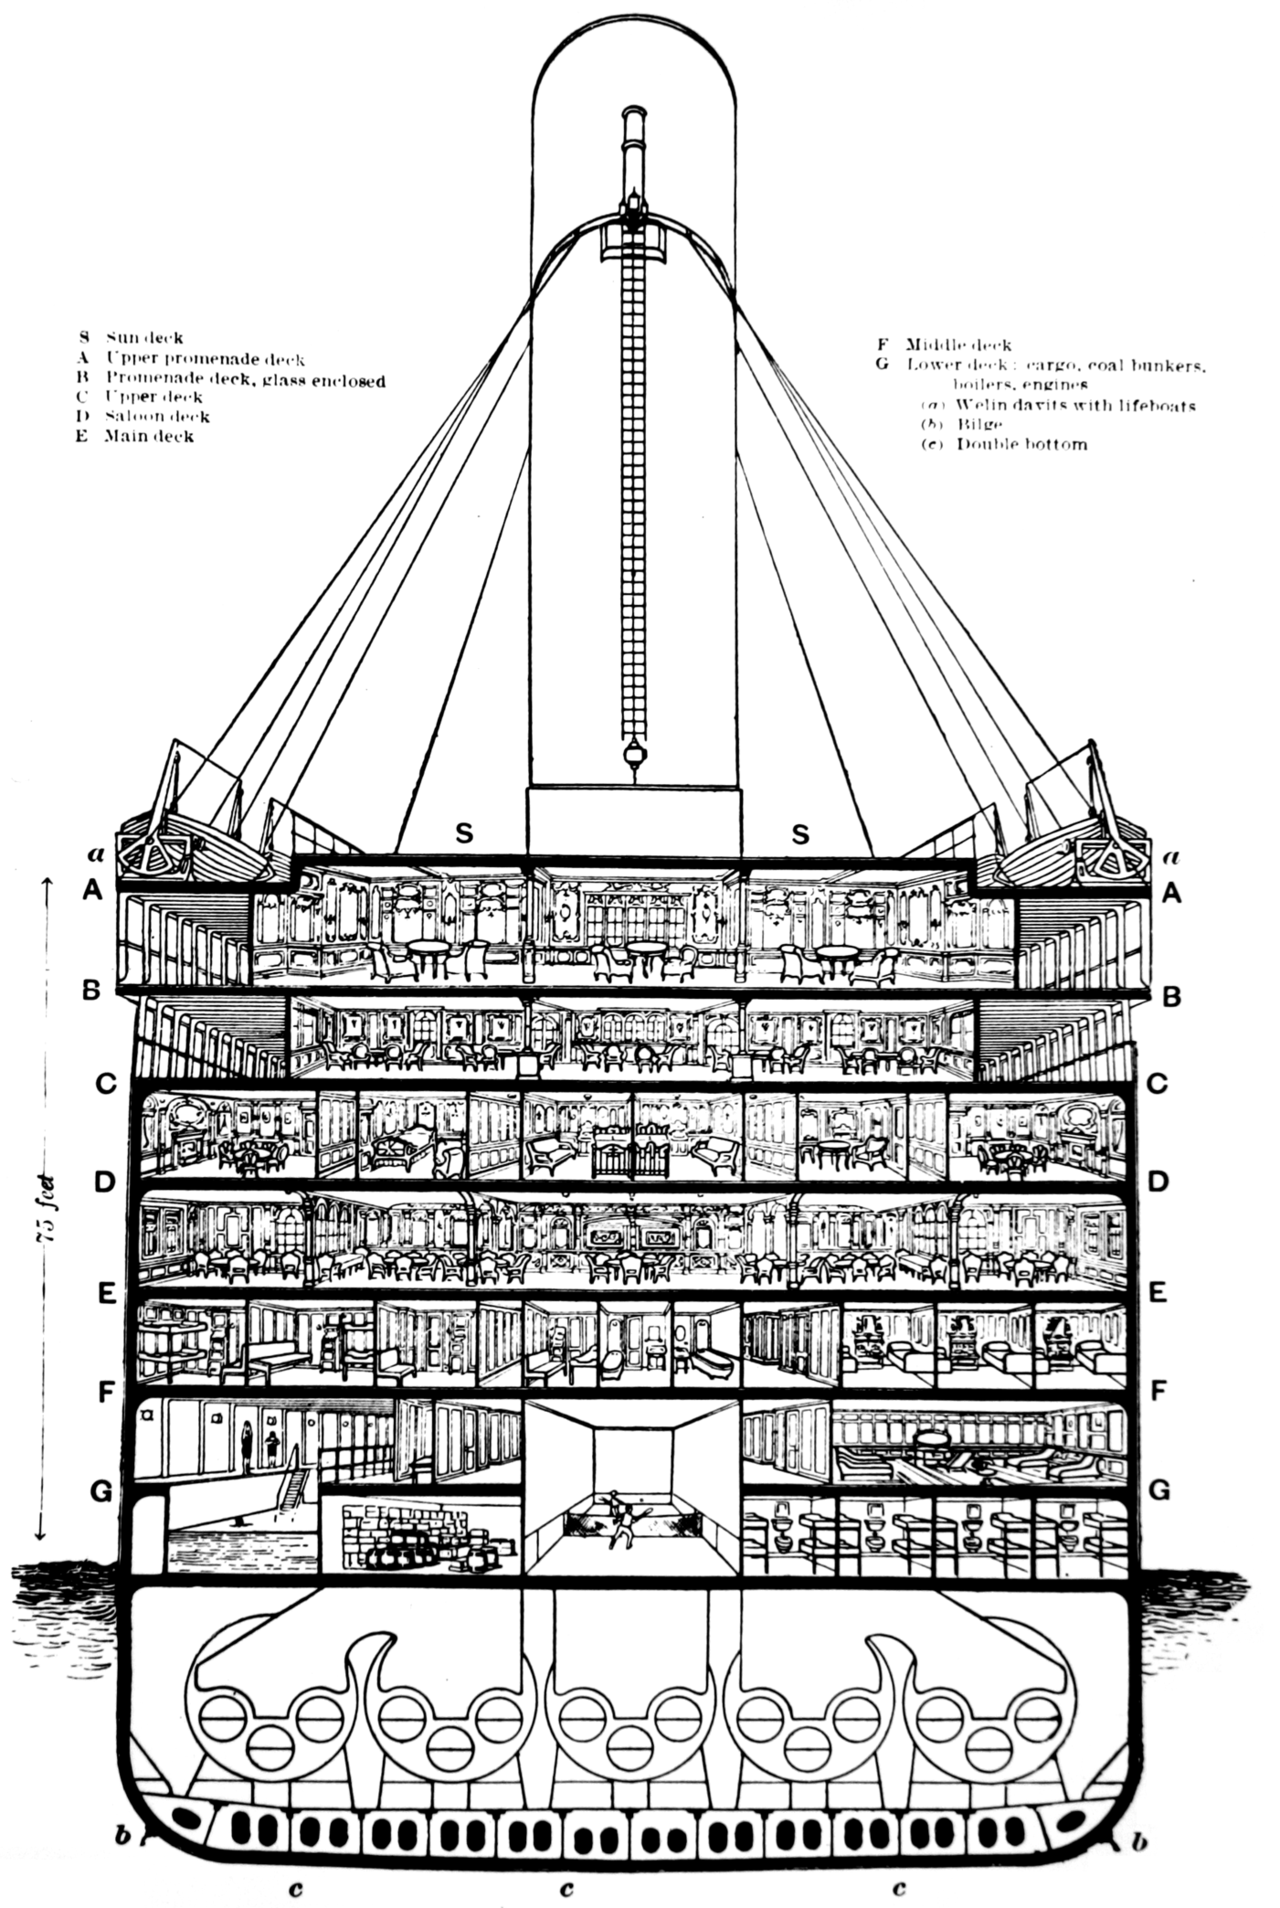
\includegraphics[scale=0.11]{./lecture_includes/titanic.png}};
      \draw[red,ultra thick,->] (6,4.25) -- (6,3.25); % Adjust the coordinates accordingly
      \node at (8,4.5) {First Class: Decks B-C}; % Adjust the position accordingly
    \end{tikzpicture}
  \end{figure}
\end{frame}

\begin{frame}{Titanic layout}
  \begin{figure}
    \begin{tikzpicture}
      \node[anchor=south west,inner sep=0] at (0,0) {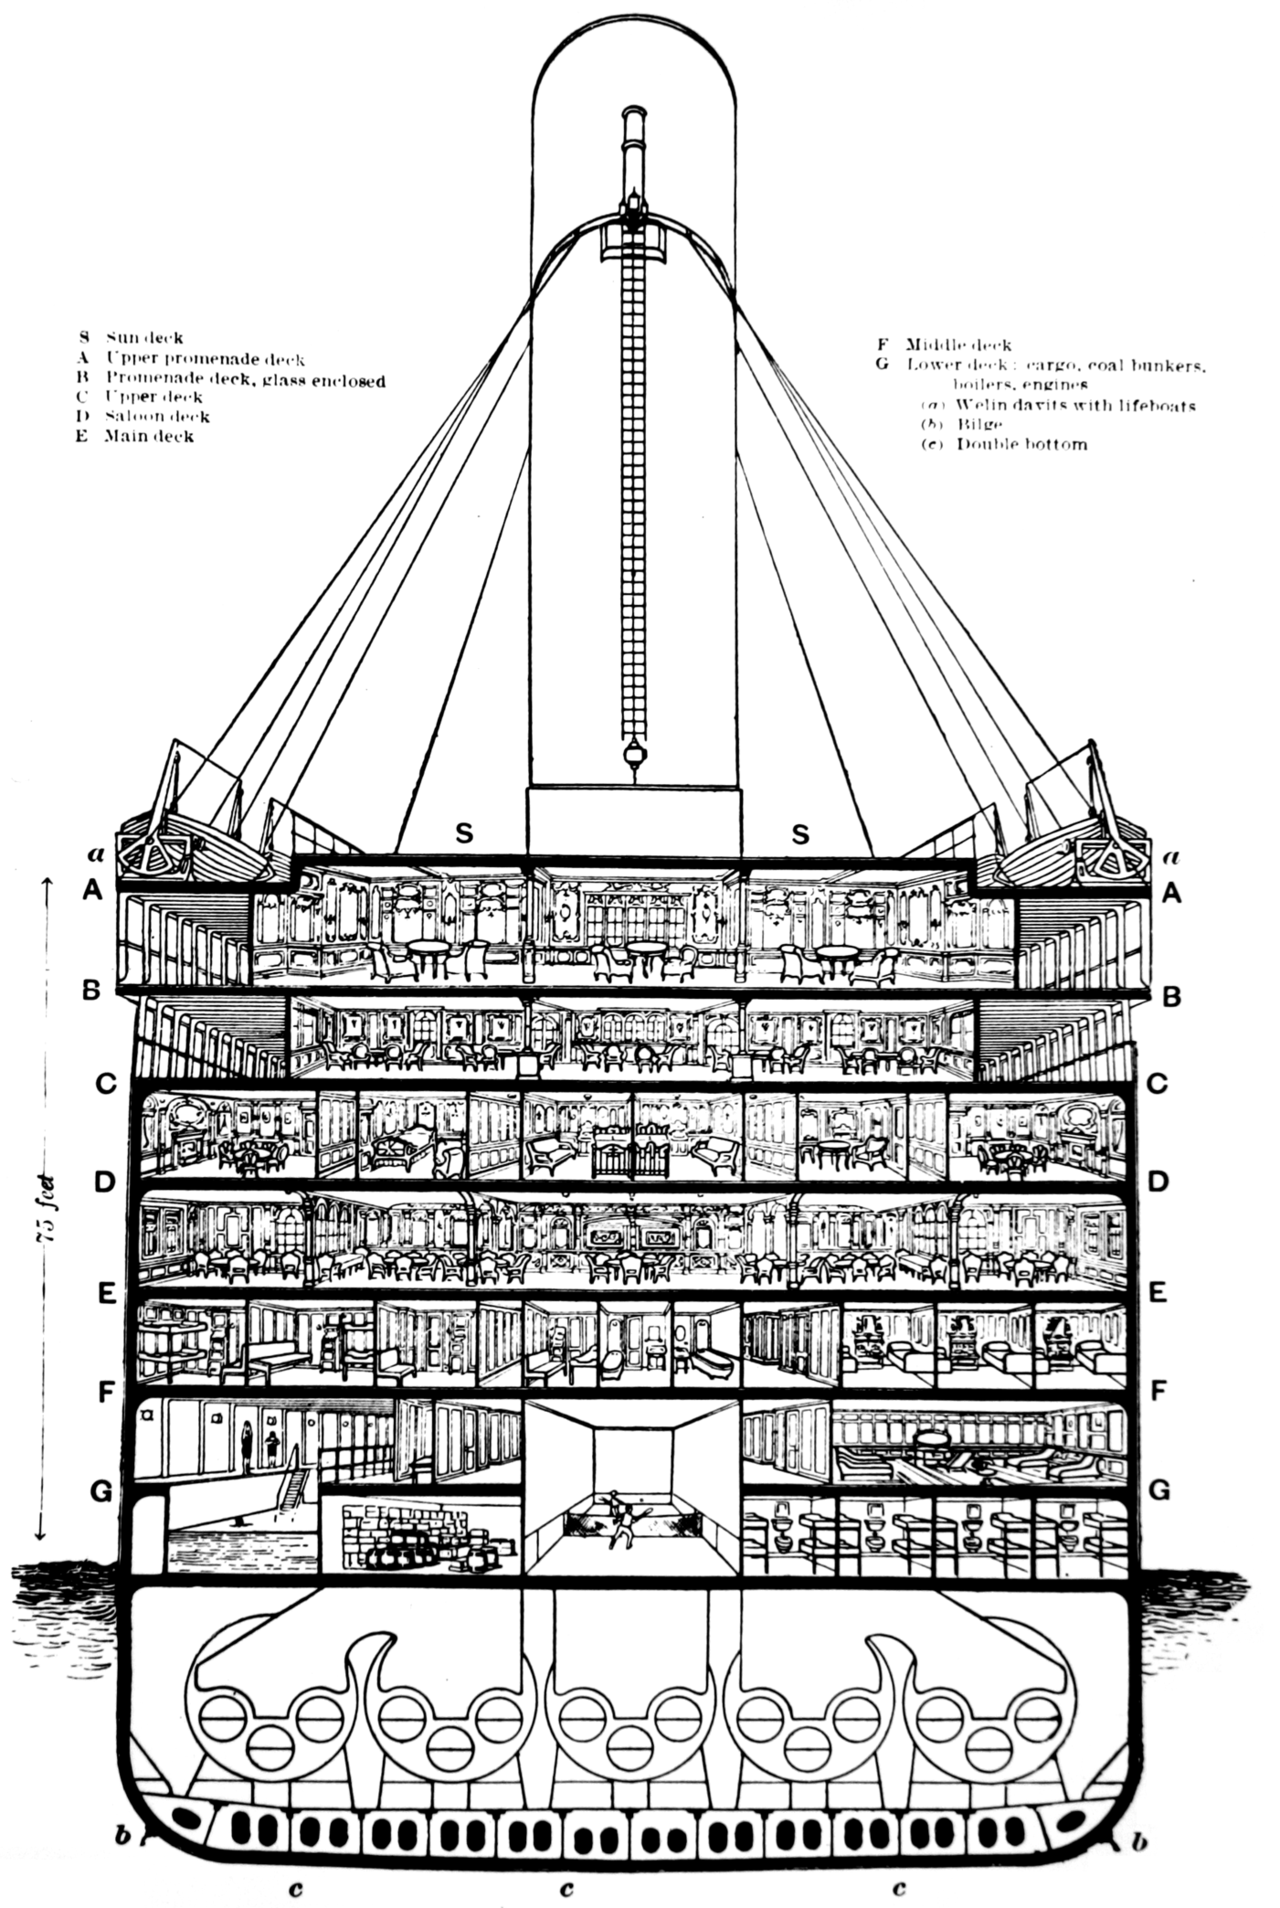
\includegraphics[scale=0.11]{./lecture_includes/titanic.png}};
      \draw[blue,ultra thick,->] (6,3.5) -- (6,2.5); % Adjust the coordinates accordingly
      \node at (8,4) {Second Class: Decks D-E}; % Adjust the position accordingly
    \end{tikzpicture}
  \end{figure}
\end{frame}

\begin{frame}{Titanic layout}
  \begin{figure}
    \begin{tikzpicture}
      \node[anchor=south west,inner sep=0] at (0,0) {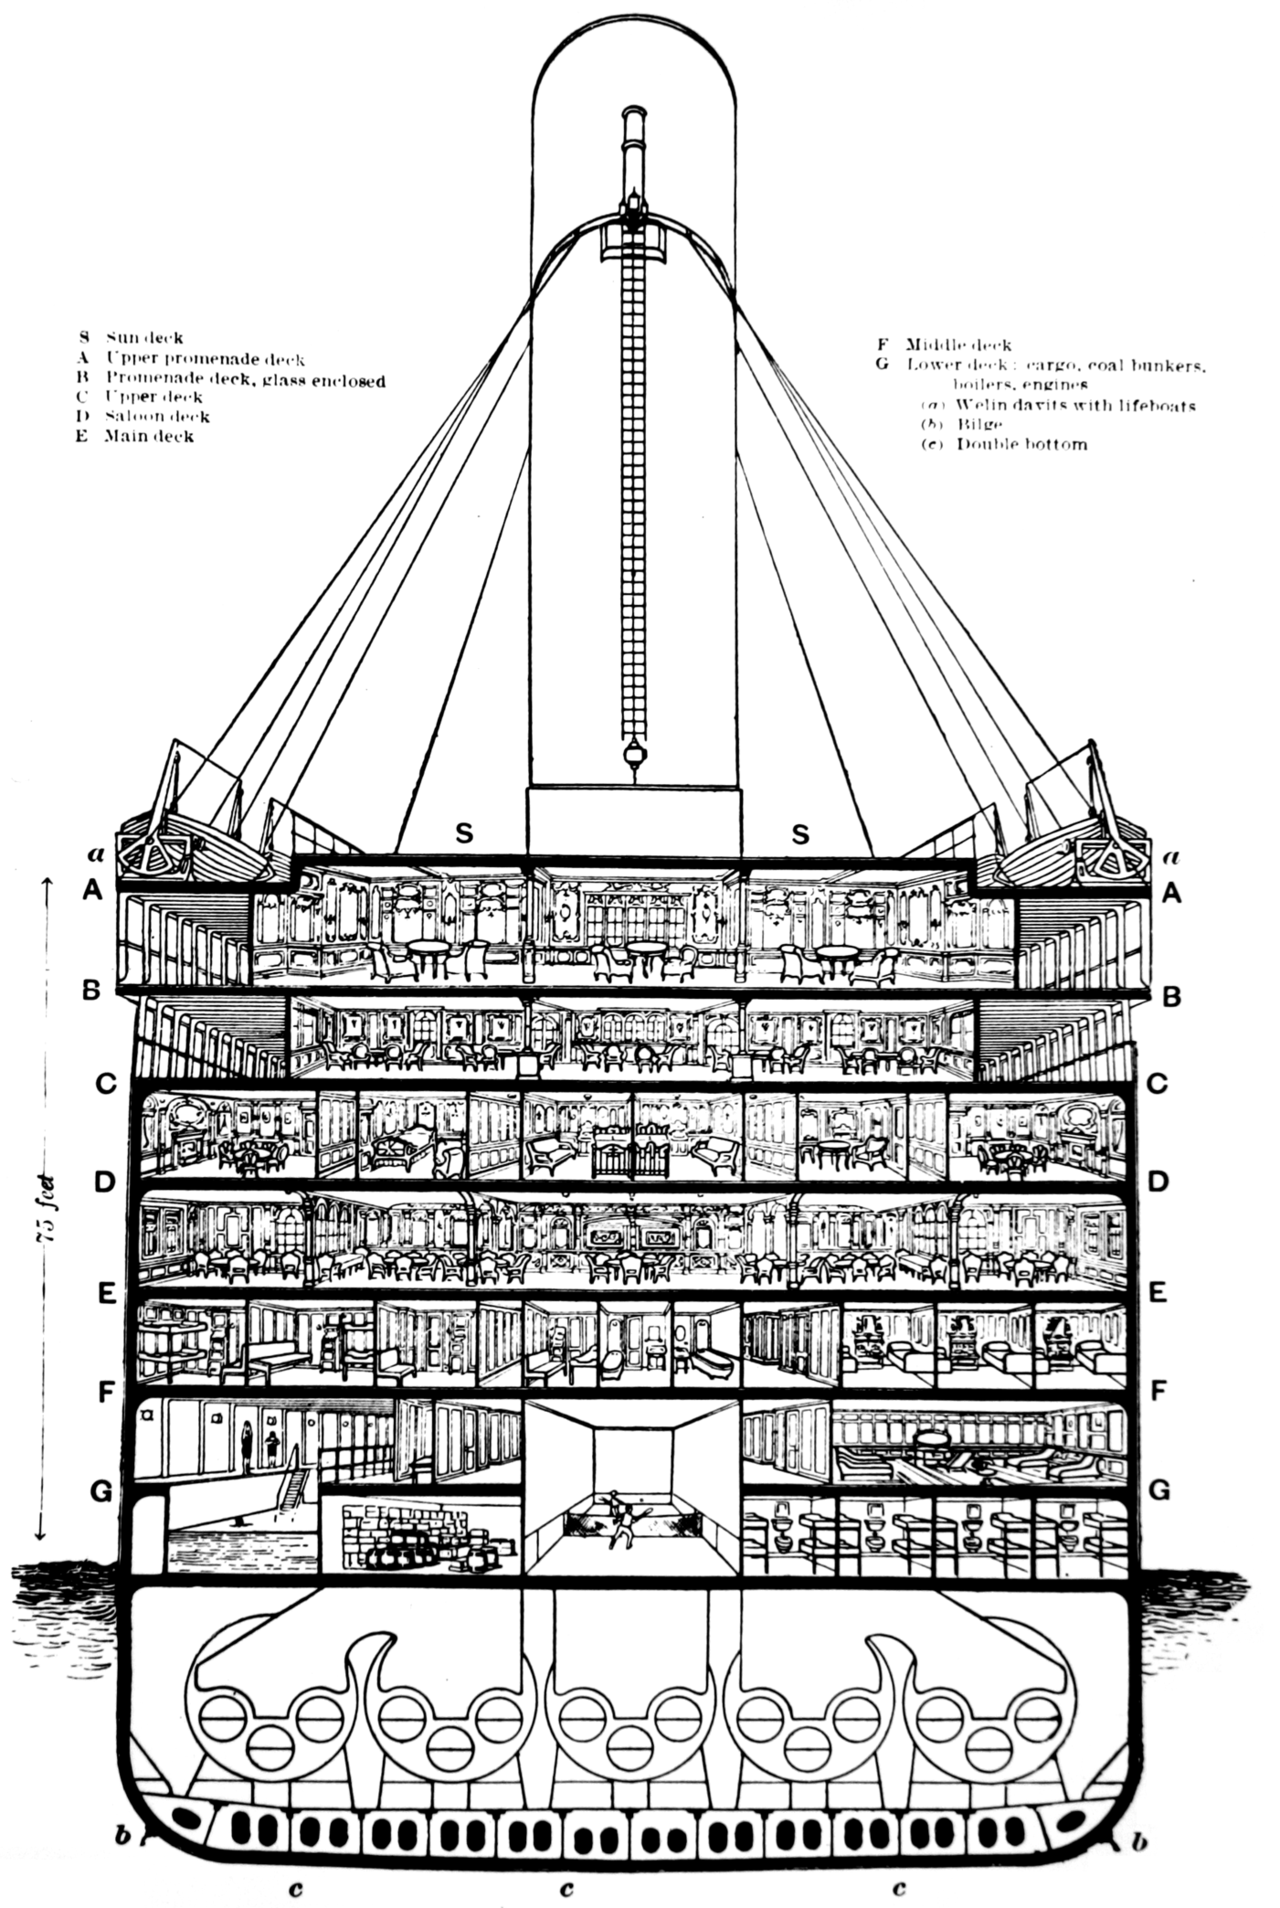
\includegraphics[scale=0.11]{./lecture_includes/titanic.png}};
      \draw[green,ultra thick,->] (6,2.25) -- (6,1.5); % Adjust the coordinates accordingly
      \node at (8,2.5) {Third Class: Decks F and G}; % Adjust the position accordingly
    \end{tikzpicture}
  \end{figure}
\end{frame}



\begin{frame}{Exercise: Titanic DAG}

\begin{figure}
\begin{center}
\caption{Women $W$ and children $C$ first maritime rule is a confounder for estimating first class $D$ effect on surviving $Y$}
\begin{tikzpicture}[node distance=2cm]
% nodes %
\node[text centered] (d) {$D$};
\node[below left of = d, text centered] (c) {$\mybox{C}$};
\node[above left of = d, text centered] (w) {$\mybox{W}$};
\node[right of = d, text centered] (y) {$Y$};
% edges %
\draw[->, line width= 1] (d) -- (y);
\draw[->, line width= 1] (c) -- (d);
\draw[->, line width= 1] (w) -- (d);
\draw[->, line width= 1] (c) -- (y);
\draw[->, line width= 1] (w) -- (y);
\end{tikzpicture}
\label{fig:titanic}
\end{center}
\end{figure}

\bigskip

Backdoor criterion can be satisfied by blocking on $W$ and $C$.  These are our known confounders.  Now we just need data to see if it's quantified.

\end{frame}

\begin{frame}{Titanic exercise}

\begin{enumerate}
\item \textbf{Stratify the confounders}: Our age and sex variables are both binary, so we can only create four strata: male children, female children, male adults, female adults
\item \textbf{Calculate differences within strata}: Calculate average survival rates for each group within each of the four strata and difference within strata
\item \textbf{Calculate probability weights}: Count the number of people in each strata and divide by the total number of souls aboard (crew and passengers)
\item \textbf{Aggregate differences across strata using weights}: Estimate the ATE by aggregating the difference in survival rates over the four strata with each strata-specific difference weighted by that strata's weight
\end{enumerate}


\end{frame}

\begin{frame}{Table 1: Typical balance table}

{\renewcommand{\arraystretch}{1.1}
\tabcolsep=1.3\tabcolsep 		
\begin{table}\small\index{rolling!3}
\caption{Differences in female and adult passengers by first class status on the Titanic. }
\centering
\begin{tabular}{lcc|cc}
\toprule
\multicolumn{1}{c}{\textbf{Variable name}}&
\multicolumn{2}{c}{\textbf{First class}}&
\multicolumn{2}{c}{\textbf{All other classes}}\\
\multicolumn{1}{c}{}&
\multicolumn{1}{c}{Obs}&
\multicolumn{1}{c}{Mean}&
\multicolumn{1}{c}{Obs}&
\multicolumn{1}{c}{Mean}\\
\midrule
Percent adult		&	325 	& 98.2\% & 1,876 & 94.5\% \\
Percent female		& 	325	& 44.6\% & 1,876 & 17.3\% \\
\bottomrule
\end{tabular}
\label{tab:titanic-age}
\end{table}}
\end{frame}


\begin{frame}{Table 2: Stratified sample}

{\renewcommand{\arraystretch}{1.1}
\tabcolsep=1.3\tabcolsep 		
\begin{table}\small\index{rolling!3}
\caption{Counts and Titanic survival rates by strata and first class status.}
\centering
\begin{tabular}{lcc|cc|c}
\toprule
\multicolumn{1}{c}{\textbf{}}&
\multicolumn{2}{c}{\textbf{First class}}&
\multicolumn{2}{c}{\textbf{All other classes}}&
\multicolumn{1}{c}{\textbf{}}\\
\multicolumn{1}{l}{Strata}&
\multicolumn{1}{c}{Obs}&
\multicolumn{1}{c}{Mean}&
\multicolumn{1}{c}{Obs}&
\multicolumn{1}{c}{Mean}&
\multicolumn{1}{c}{Total}\\
\midrule
Male adult		& 175	& 0.326	& 1,492	& 0.188	& 1,667 \\
Female adult	& 144	& 0.972	& 281	& 0.626	& 425 \\
Male child		& 5		& 1		& 59		& 0.407 	& 64\\
Female child	& 1		& 1		& 44		& 0.613 	& 45\\
\midrule
Total	observations	& 325	&&	1,876	 && 2,201\\
\bottomrule
\end{tabular}
\label{tab:titanic-counts}
\end{table}}


\end{frame}

\begin{frame}{Table 3: Estimates of aggregate parameters}

{\renewcommand{\arraystretch}{1.1}
\tabcolsep=1.3\tabcolsep 		
\begin{table}\tiny\index{rolling!3}
\caption{Differences in survival rates, stratification weights, and estimates of parameters}
\centering
\begin{tabular}{lc|ccc}
\toprule
\multicolumn{1}{l}{\textbf{Strata}}&
\multicolumn{1}{c}{\textbf{Differences in Survival Rates}}&
\multicolumn{1}{c}{\textbf{Weight$_{k,ATE}$}}&
\multicolumn{1}{c}{\textbf{Weight$_{k,ATT}$}}&
\multicolumn{1}{c}{\textbf{Weight$_{k,ATU}$}}\\
\midrule
Male adult		& 0.138 &	0.76 &	0.54	&0.80	\\
Female adult	& 0.346 &	0.19 &	0.44	&0.15	\\
Male child		& 0.593 &	0.03 &	0.02	&0.03	\\
Female child	& 0.387 &	0.02 &	0.00	&0.02	\\
\midrule
\multicolumn{1}{l}{\textbf{}}&
\multicolumn{1}{c}{\textbf{No stratification}}&
\multicolumn{3}{c}{\textbf{Stratification weighted estimates}}\\

 & $\widehat{\textbf{SDO}}$& $\widehat{\textbf{ATE}}$ & $\widehat{\textbf{ATT}}$ & $\widehat{\textbf{ATU}}$ \\
\midrule
\textbf{Estimated coefficient}& 0.35 & 0.20 & 	0.24	 & 0.19   \\
\bottomrule
\end{tabular}
\label{tab:titanic-weights}
\end{table}}



\end{frame}



\begin{frame}{Curse of dimensionality}

\begin{itemize}
\item We were able to estimate all three causal effect parameters because for all four strata there were units in both treatment and control
\item But if we dropped the only female child in first class from the data, we'd be in trouble bc there wouldn't be any way to calculate a difference for that group
\item This happens when you have many covariates or some are continuous -- it's called curse of dimensionality
\item If we do not have at least one observation in both treatment and control for \emph{all covariate strata}, then some of parameters cannot be estimated due to losing support

\end{itemize}

\end{frame}

\begin{frame}

\begin{table}\small\index{rolling!3}
\caption{Counts and Titanic survival rates by strata and first class status.}
\centering
\begin{tabular}{lcc|cc|c}
\toprule
\multicolumn{1}{c}{\textbf{}}&
\multicolumn{2}{c}{\textbf{First class}}&
\multicolumn{2}{c}{\textbf{All other classes}}&
\multicolumn{1}{c}{\textbf{}}\\
\multicolumn{1}{l}{Strata}&
\multicolumn{1}{c}{Obs}&
\multicolumn{1}{c}{Mean}&
\multicolumn{1}{c}{Obs}&
\multicolumn{1}{c}{Mean}&
\multicolumn{1}{c}{Total}\\
\midrule
Male adult		& 175	& 0.326	& 1,492	& 0.188	& 1,667 \\
Female adult	& 144	& 0.972	& 281	& 0.626	& 425 \\
Male child		& 5		& 1		& 59		& 0.407 	& 64\\
Female child	& 0		& n/a		& 44		& 0.613 	& 44\\
\midrule
Total	observations	& 324	&&	1,876	 && 2,200\\
\bottomrule
\end{tabular}
\label{tab:titanic-counts2}
\end{table}

\end{frame}

\begin{frame}{ATT is the only one we can get}

\begin{eqnarray}
\widehat{\delta}_{ATT} &=& (0.137 \times 0.54) + (0.346 \times 0.44) + (0.593 \times 0.02)  \nonumber \\
&=& 0.24\text{ or 24 percentage points}
\end{eqnarray}

\end{frame}

\begin{frame}

\begin{table}\tiny\index{rolling!3}
\caption{Differences in survival rates, stratification weights, and estimates of parameters without perfect stratification}
\centering
\begin{threeparttable}
\begin{tabular}{lc|ccc}
\toprule
\multicolumn{1}{l}{\textbf{Strata}}&
\multicolumn{1}{c}{\textbf{Differences in Survival Rates}}&
\multicolumn{1}{c}{\textbf{Weight$_{k,ATE}$}}&
\multicolumn{1}{c}{\textbf{Weight$_{k,ATT}$}}&
\multicolumn{1}{c}{\textbf{Weight$_{k,ATU}$}}\\
\midrule
Male adult		& 0.137 	&	0.76 &	0.54	&0.80	\\
Female adult	& 0.346 	&	0.19 &	0.44	&0.15	\\
Male child		& 0.593 	&	0.03 &	0.02	&0.03	\\
Female child	& n/a 	&	n/a 	&	n/a	&0.02	\\
\midrule
\multicolumn{1}{l}{\textbf{}}&
\multicolumn{1}{c}{\textbf{No stratification}}&
\multicolumn{3}{c}{\textbf{Stratification weighted estimates}}\\

 & $\widehat{\textbf{SDO}}$& $\widehat{\textbf{ATE}}$ & $\widehat{\textbf{ATT}}$ & $\widehat{\textbf{ATU}}$ \\
\midrule
\textbf{Estimated coefficient}& 0.35 & n/a & 	0.24	 & n/a  \\
\bottomrule
\end{tabular}
\begin{tablenotes}
\tiny
\item 
Differences in survival rates, stratification weights, and estimated parameters. All coefficients should be multiplied by 100 to get a percentage point change in survival rate as a result of having a first class cabin. Note that the SDO is a simple difference in mean outcomes and therefore \emph{not} a weighted average over the strata differences.  But the estimated ATE, ATT and ATU parameters are weighted averages in difference in means using corresponding stratification weights. 
\end{tablenotes}
\end{threeparttable}
\label{tab:titanic-weights2}
\end{table}


\end{frame}

\begin{frame}{Curse of Dimensionality}
	
	\begin{itemize}
	\item Assume we have $k$ covariates and we divide each into 3 coarse categories (e.g., age: young, middle age, old; income: low, medium, high, etc.)
	\item The number of strata is $3^k$. For $k=10$, then it's $3^{10}=59,049$
	\item The curse of dimensionality is based on the slices of all interactions of the covariates, not just the covariates, and that explodes fast
	\end{itemize}
\end{frame}


\begin{frame}{Empty cells}
	
	\begin{itemize}
	\item When some strata is empty, it means there's no one in that cell -- so maybe you don't have any female children in first class, but you do have them in other cabins
	\item When you have empty cells, you can't match within that dimension of the data, which is the "curse of dimensionality" -- more covariates makes it happen
	\item Matching methods really force us to see these curses; they're often hidden from OLS because OLS (as we'll see) overcomes the problem by just assuming a linearity (it doesn't match; it extrapolates)
	\end{itemize}
\end{frame}	







\subsection{Exact and Inexact Matching}


\begin{frame}{Common support vs no common support}

\begin{itemize}
\item Common support is what will determine unbiasedness in nonparametric methods that satisfy unconfoundedness
\item Strictly speaking common support will mean that we have \emph{exact} matches
\item When we have inexact matches, then nonparametric matching methods may become biased
\item Some bias adjustment methods can improve estimation
\item We'll review these all now
\end{itemize}

\end{frame}



\begin{frame}{Exact matching}

\begin{figure}[!t]\centering
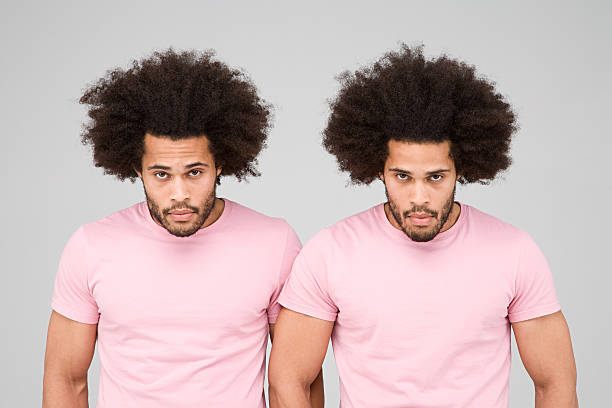
\includegraphics[scale=1.1]{./lecture_includes/identical_twins}
\end{figure}

\end{frame}

\begin{frame}{Exact Matching}


Matching goes back at least to Rubin's early work on the propensity score, but we will start with nearest neighbor matching as there's ideas there we draw upon later with synth I want to emphasize

\bigskip

Matching will match a treated unit to a comparison unit that is identical on the known and quantified confounders

\bigskip

If we can't find one, it means common support failed, the estimate would need to use nearest neighbors (with matching bias), which we will discuss



\end{frame}



\begin{frame}{Training example (unmatched)}

\begin{figure}[!t]\centering
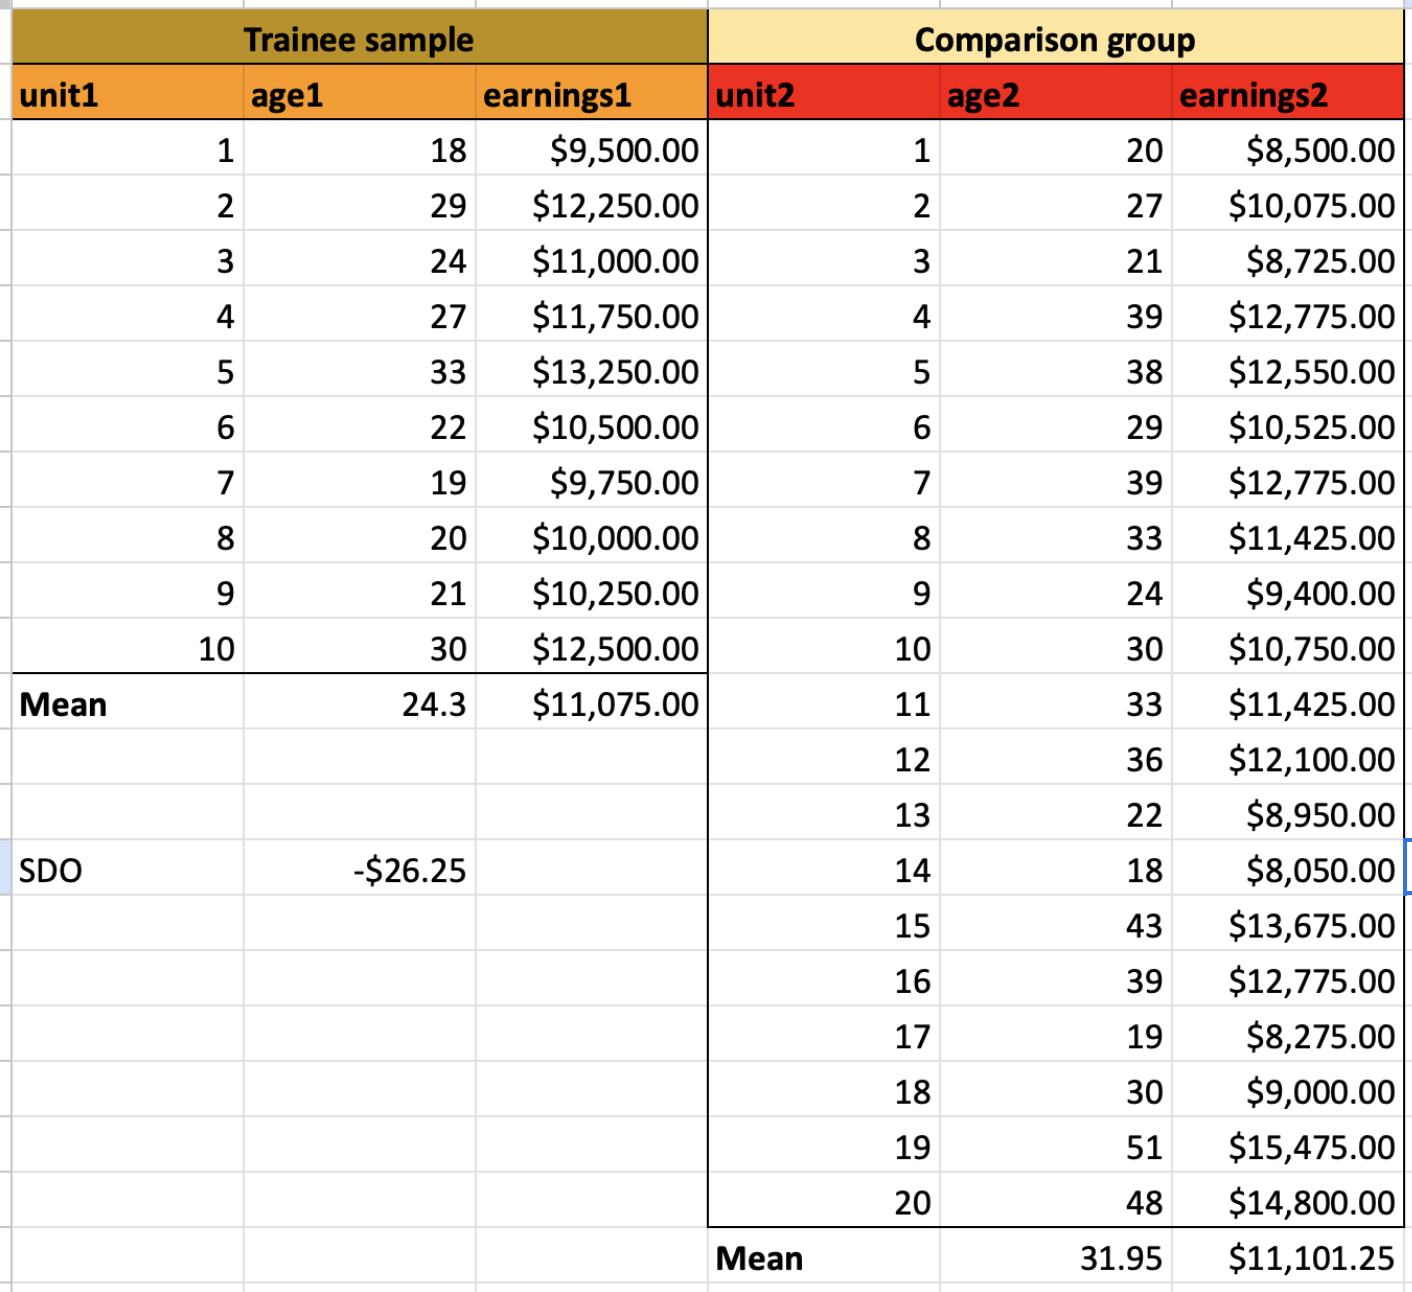
\includegraphics[scale=0.35]{./lecture_includes/raw_example}
\end{figure}


\end{frame}


\begin{frame}{Age Imbalance}

\begin{figure}[!t]\centering
\caption{Age distribution of a job training program's trainees (green) versus a sample of workers who were not enrolled in the trainee program (white).}
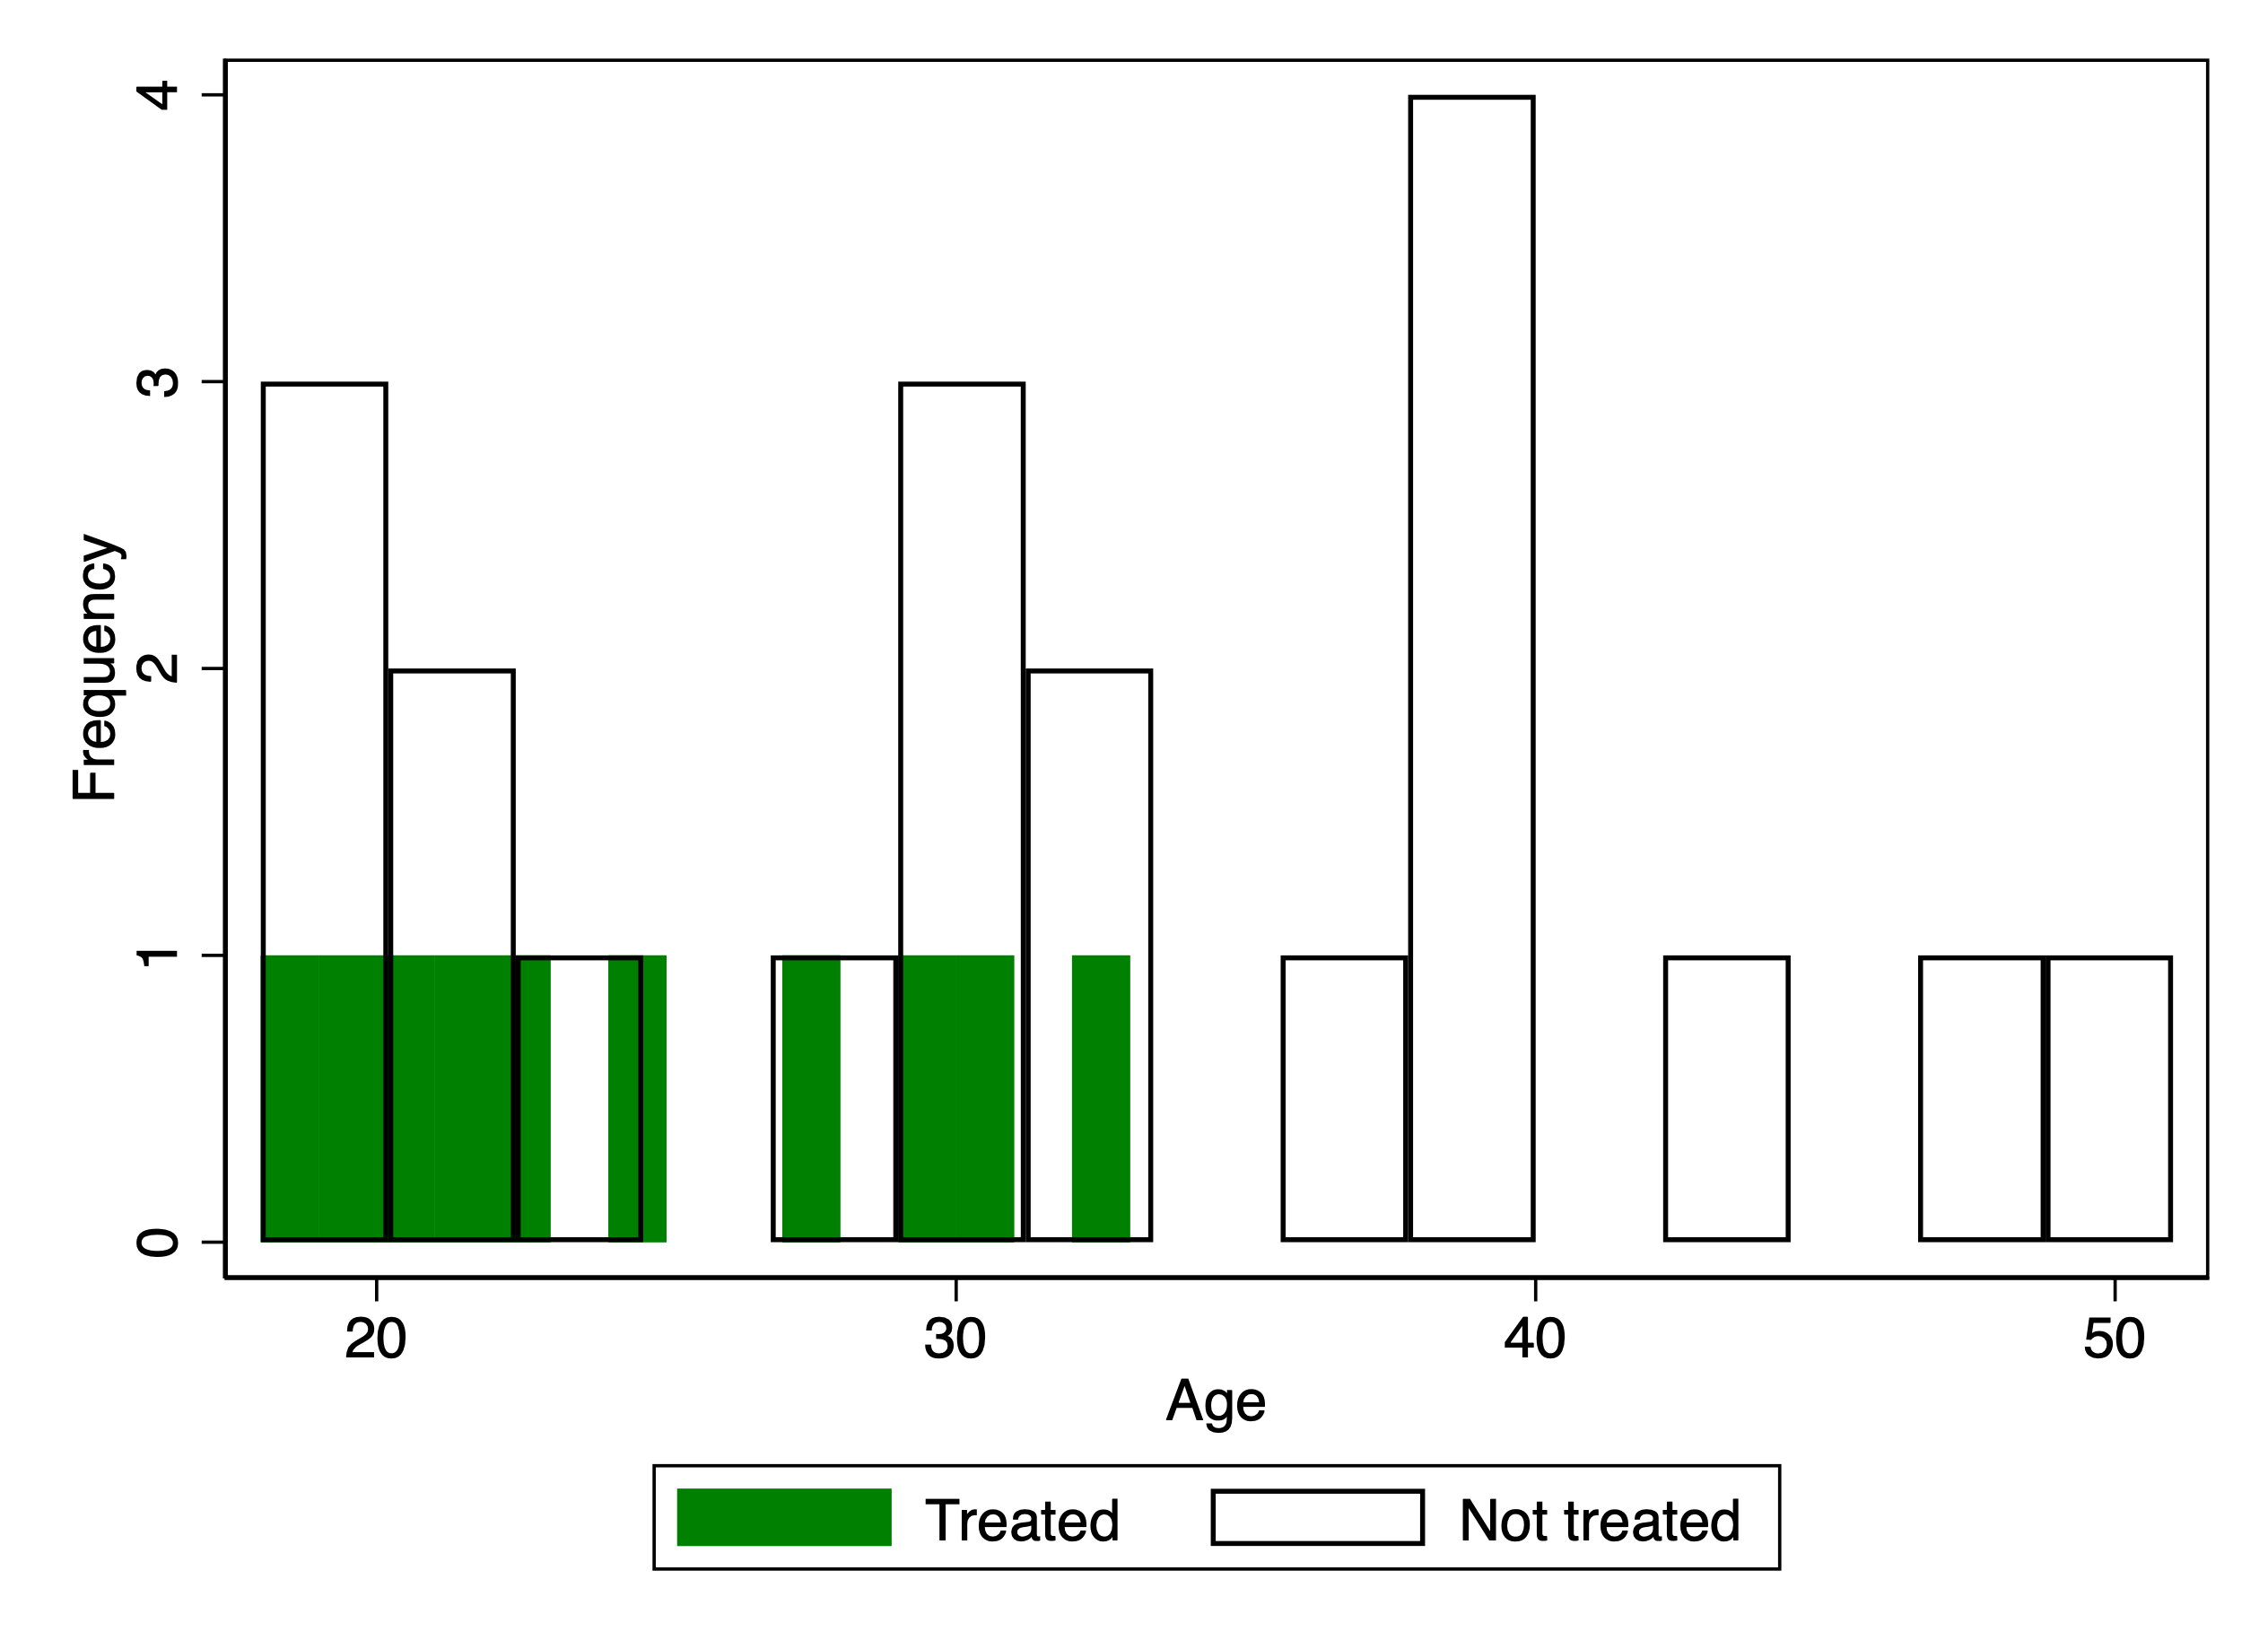
\includegraphics[scale=0.20]{./lecture_includes/age_match.png}
\end{figure}

\end{frame}

\begin{frame}{Simple example}

Let's review together \texttt{nnmatch.do} to see how we do this using a program called \texttt{teffects nnmatch} in Stata. Focus only on the first ten lines and pay attention to who got matched to who.  Calculate the answers by hand. 


\end{frame}


\begin{frame}{Exact matching}

\begin{itemize}
\item Exact matching finds a person in the control group whose value of $X_j$ is \emph{exactly} equal to each person in the treatment group $i$
\item Will not work if the conditioning set includes a continuous variable
\item Will also not work if $K$ gets large (curse of dimensionality we discuss later)
\item Numerically identical to subclassification
\end{itemize}

\end{frame}



\begin{frame}{ATT estimator}

We will focus on the ATT for the rest of today and the equation is:

\begin{equation}
\widehat{ATT} = \dfrac{1}{N_T} \sum_{D_i=1}(Y_i - Y_{j(i)})
\label{eq:att_simplematch}
\end{equation}

where $Y_{j(i)}$ is the $j$\textsuperscript{th} unit matched to the $i$\textsuperscript{th} unit based on the $j$\textsuperscript{th} being ``exactly equal to'' the $i$\textsuperscript{th} unit with respect to the $X$ conditioning set

\end{frame}

\begin{frame}{Number of matches}

What if I find two or more $M$ units with the identical $X$ value? Then what?

\begin{equation}
\widehat{ATT} = \dfrac{1}{N_T} \sum_{D_i=1} \bigg ( Y_i - \bigg [\dfrac{1}{M} \sum_{m=1}^M Y_{j_m(1)} \bigg ] \bigg )
\label{eq:att_match}
\end{equation}

\bigskip

Notice that we are only dealing with $Y^0_i$ by matching; The $Y^1_i$ is fine as is.

\end{frame}

\begin{frame}{Matching algorithm}

\begin{enumerate}
\item For each unit $i$ in the treatment group with known and quantified confounder $X=x_i$, find all units $j$ in the donor pool for whom $x_i=x_j$. These $j$ units are our $M$ matches and $M$ can be one or it can be greater than one if you want it to be.
\item For each unit $i$, replace its missing potential outcome, $Y^0_i$, with the matched $j$ units' realized outcomes, $\frac{1}{M} \sum {Y}_{j(i)}$, from Step 1. Do this for all $i$ units in the treatment group.
\item For each unit $i$, calculate the difference between realized earnings and matched earnings, $\widehat{\delta}_i=Y_i - \frac{1}{M} \sum {Y}_{j(i)}$.
\item Finally, estimate the sample ATT by averaging over all $i$ differences in earnings from Step 3 as $\frac{1}{N_T} \sum \widehat{\delta}_i$, where $N_T$ is the number of treatment units.
\end{enumerate}

\end{frame}



\begin{frame}{Matched sample}

\begin{figure}[!t]\centering
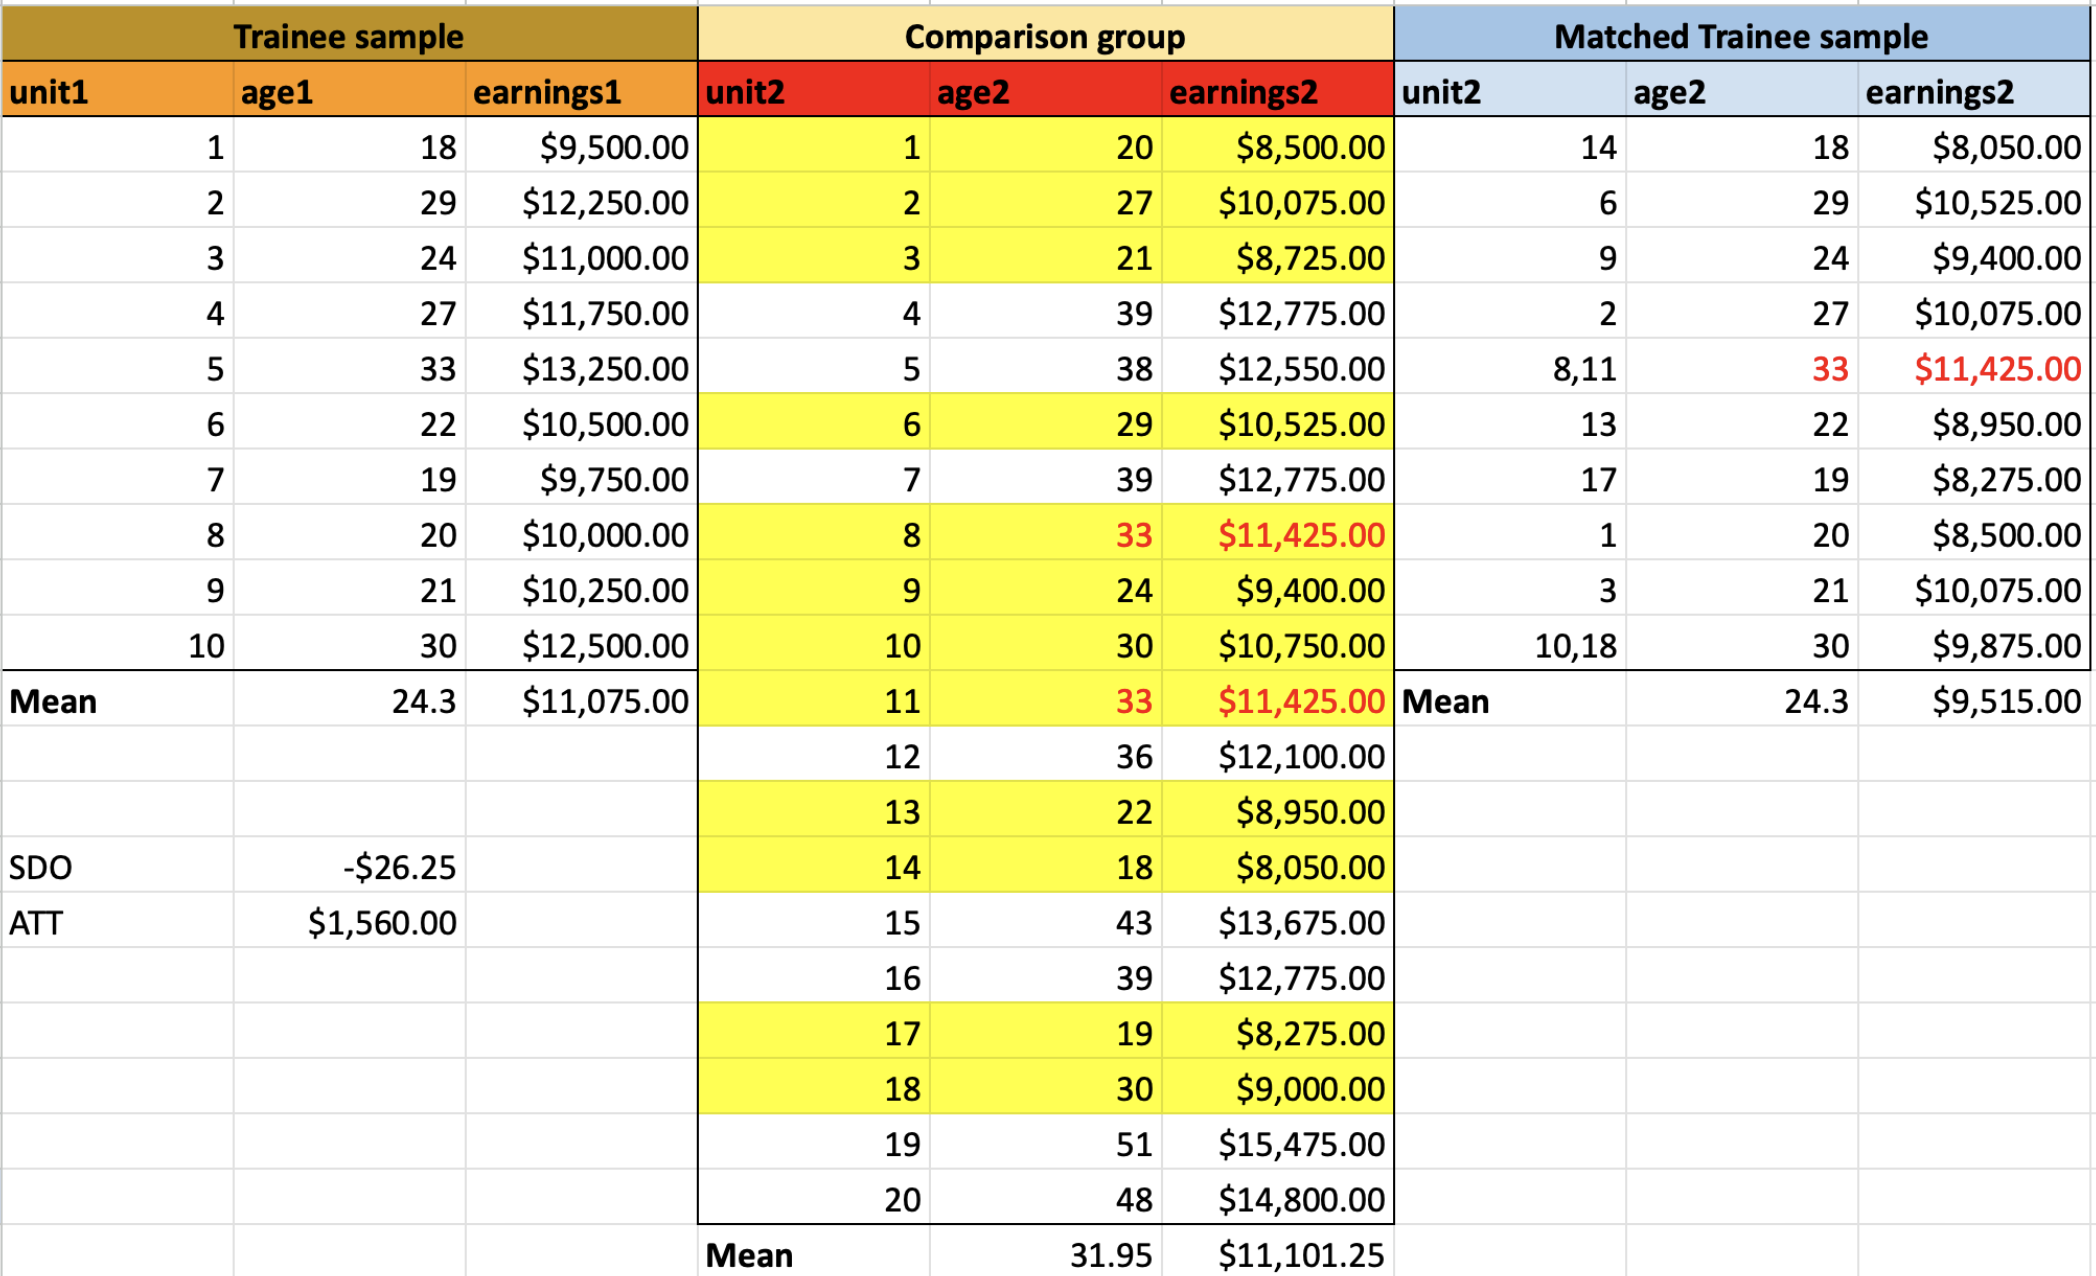
\includegraphics[scale=0.3]{./lecture_includes/matched_example}
\end{figure}



\end{frame}

\begin{frame}{Matched sample}

\begin{itemize}
\item Notice how you don't use all the data with matching (only the yellow units)
\item That's because not all of the data is relevant or helpful
\item This is an important point -- not all of the data in causal inference has the variation you need for estimating causal effects
\item You're imputing missing counterfactuals, not predicting outcomes -- it's a different task
\end{itemize}

\end{frame}




\begin{frame}{Inexact matching}

\begin{figure}[!t]\centering

\includegraphics[scale=0.75]{./lecture_includes/fraternal_twins}
\end{figure}

\end{frame}


\begin{frame}{Curse of Dimensionality}
	
	\begin{itemize}
	\item If no matches can be found, it means many cells may contain either only treatment units or only control units but not both ("empty cells") which violates our common support assumption
	\item Sometimes people want to "bin" or "coarsen" the covariates, and you can do that, but then it's no longer exact matching and any differences in potential outcomes across the units still create biases
	\item So here we look at inexact matches and then we look at ways to reduce the matching biases when common support fails
	\end{itemize}
\end{frame}	






\begin{frame}{Nearest Neighbor Matching}
	
	\begin{itemize}
	\item Estimate $\widehat{ATT}$ by \emph{imputing} the missing potential outcome of each treatment unit $i$ using the observed outcome from that outcome's ``nearest'' neighbor $j$ in the control set using $X$ for the matching
		\begin{eqnarray*}
		\widehat{ATT} = \frac{1}{N_T}\sum_{D_i=1} (Y_i - Y_{j(i)})
		\end{eqnarray*}where $Y_{j(i)}$ is the observed outcome of a control unit such that $X_{j(i)}$ is the \textbf{closest} value to $X_i$ among all of the control observations (eg match on $X$)
	\end{itemize}
\end{frame}

\begin{frame}{Matching}
	
	\begin{itemize}
	\item We could also use the average observed outcome over $M$ closest matches:
		\begin{eqnarray*}
		\widehat{ATT} = \frac{1}{N_T}\sum_{D_i=1}\left(Y_i-\left[\frac{1}{M}\sum_{m=1}^MY_{j_m(1)}\right]\right)
		\end{eqnarray*}
	\item Works well when we can find good matches for each treatment group unit, so $M$ is usually defined to be small (i.e., $M=1$ or $M=2$)
	\end{itemize}
\end{frame}



\begin{frame}{Matching example with single covariate}
	
	\begin{table}
	\begin{tabular}{c|c|c|c|c}
	\hline
	$i$ & $Y^1_i$ & $Y^0_i$ & $D_i$ & $X_i$ \\
	\hline
	1 & 6 &  \textcolor{red}{?} & 1 & 3 \\
	2 & 1 &  \textcolor{red}{?} & 1 & 1 \\
	3 & 0 &   \textcolor{red}{?} & 1 & 10 \\
	\hline
	4 &  & 0 & 0 & 2 \\
	5 &  & 9 & 0 & 3 \\
	6 &  & 1 & 0 & -2 \\
	7 &  & 1 & 0 & -4 \\
	\hline
	\end{tabular}
	\end{table}
	
	
	\begin{flalign*}
		    \only<1-2>{&\text{Question: What is }\widehat{ATT}=\frac{1}{N_T} \sum_{D_i=1} (Y_i - Y_{j(i)})\text{?}}& \\
		    \only<2-2>{&\text{Match and plug in!}} \\
 	\end{flalign*}

\end{frame}
	
	
\begin{frame}{Matching example with single covariate}
	
	\begin{table}
	\begin{tabular}{c|c|c|c|c}
	\hline
	$i$ & $Y^1_i$ & $Y^0_i$ & $D_I$ & $X_i$ \\
	\hline
	1 & 6 &  \textcolor{blue}{9} & 1 & \textcolor{blue}{3} \\
	2 & 1 &  \textcolor{green}{0} & 1 & \textcolor{green}{1} \\
	3 & 0 &   \textcolor{blue}{9} & 1 & \textcolor{blue}{10} \\
	\hline
	4 &  & \textcolor{green}{0} & 0 & \textcolor{green}{2} \\
	5 &  & \textcolor{blue}{9} & 0 & \textcolor{blue}{3} \\
	6 &  & 1 & 0 & -2 \\
	7 &  & 1 & 0 & -4 \\
	\hline
	\end{tabular}
	\end{table}
	
	
	\begin{flalign*}
		&\text{Question: What is }\widehat{\delta_{ATT}}=\frac{1}{N_T} \sum_{D_i=1} (Y_i - Y_{j(i)})\text{?}& \\
		&\widehat{ATT} = \frac{1}{3} \cdot (6-\textcolor{blue}{9}) + \frac{1}{3} \cdot (1-\textcolor{green}{0}) + \frac{1}{3} \cdot (0-\textcolor{blue}{9}) = -3.7
	\end{flalign*}

\end{frame}


%{
%\setbeamercolor{background canvas}{bg=}
%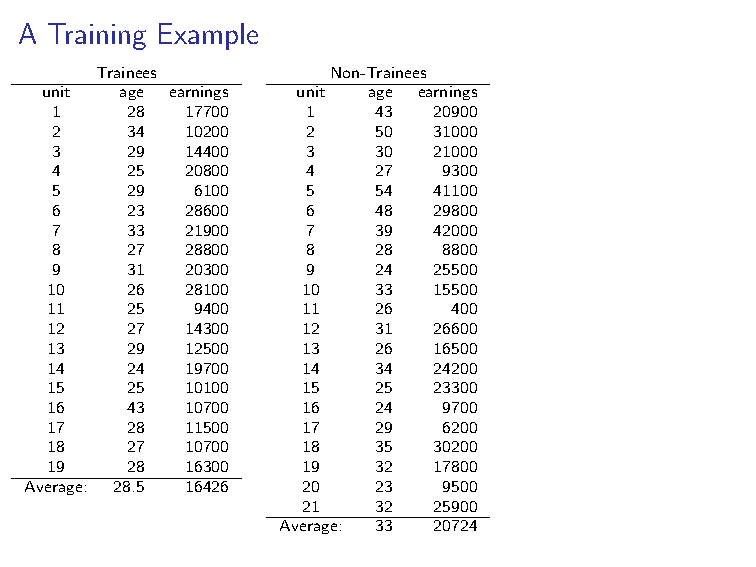
\includepdf[pages=1-last]{./lecture_includes/abadie-matching2.pdf}
%}



\begin{frame}{Measuring the matching discrepancy}

\begin{itemize}
\item What does it mean to be close when I am working with a large number of covariates?
\item What if we had a way of measuring a match in terms of how ``close'' each unit's $X_i$ value was to the matched $X_j$
\item Let's do that and use the square root of the sum of all squared differences in each unit's $X_i - X_{j(i)}$ as a measure of how bad the match is
\item This is called the Euclidean distance
\end{itemize}


\end{frame}

%\begin{frame}{Alternative distance metric: Euclidean distance}
	
% When the vector of matching covariates, $X= \colvec{X_1\\X_2\\\vdots\\X_k}$ has more than one dimension ($k>1$) we will need a new definition of \textbf{distance} to measure ``closeness''.  
%\end{frame}

\begin{frame}{Euclidean distance}
	\begin{block}{Definition: Euclidean distance}
    \vspace*{-2.5mm}
    \begin{eqnarray*}
    ||X_i-X_j|| &=& \sqrt{ (X_i-X_j)'(X_i-X_j) } \\
    &=& \sqrt{ \sum_{n=1}^k (X_{ni} - X_{nj})^2 }
    \end{eqnarray*}
    \vspace*{-2.5mm}
	\end{block}
	
Let's do this together -- sometimes it helps to manually calculate this

\bigskip

\url{https://docs.google.com/spreadsheets/d/1iro1Qzrr1eLDY_LJVzOYvnQZWmxY8JyTcDf6YcdhkwQ/edit?usp=sharing}

	
\end{frame}

\begin{frame}{Visualization of Optimal Match}

\begin{figure}[!t]\centering
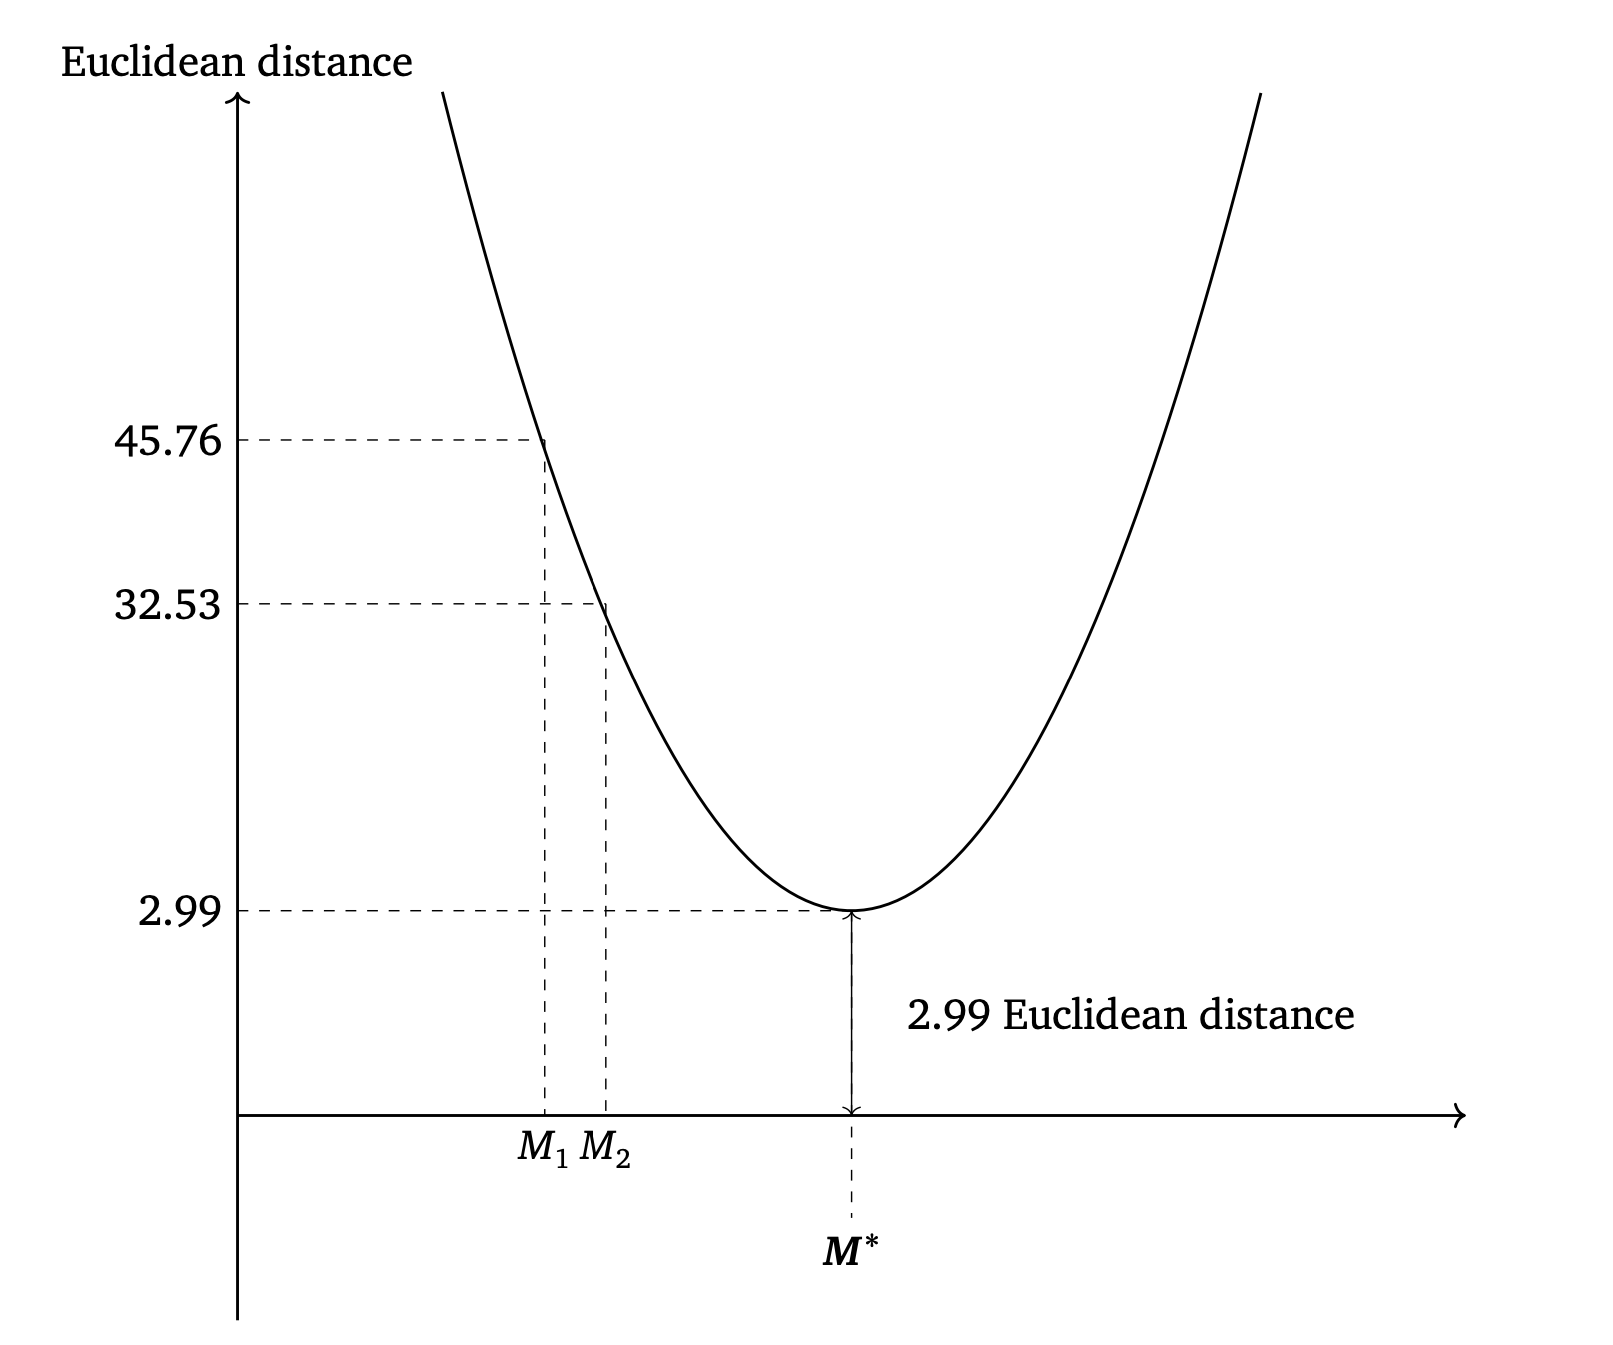
\includegraphics[scale=0.35]{./lecture_includes/optimal_match}
\end{figure}

\end{frame}



%\begin{frame}{Inexact matching: Random match 1}

%\begin{figure}[!t]\centering
%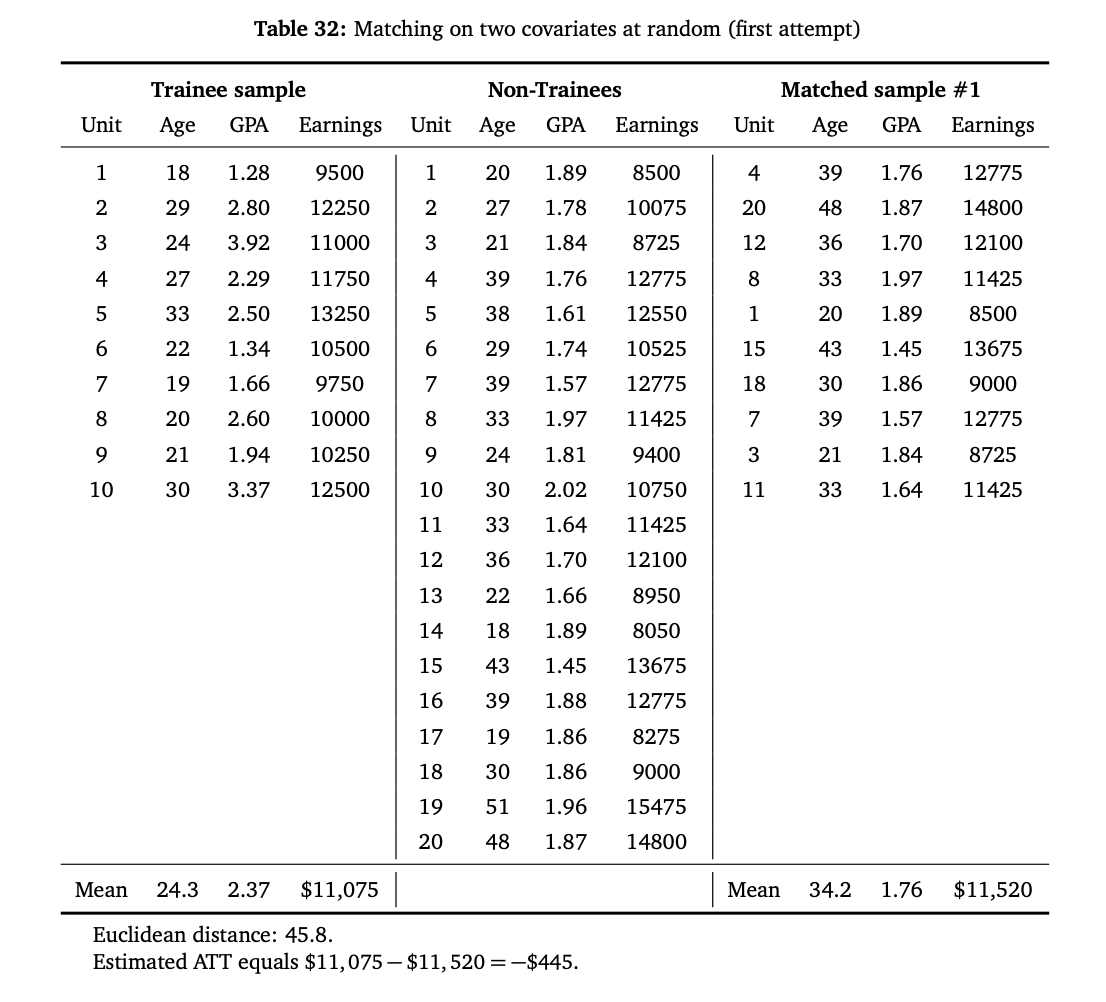
\includegraphics[scale=0.45]{./lecture_includes/inexact_random1}
%\end{figure}

%\end{frame}


%\begin{frame}{Inexact matching: Random match 2}

%\begin{figure}[!t]\centering
%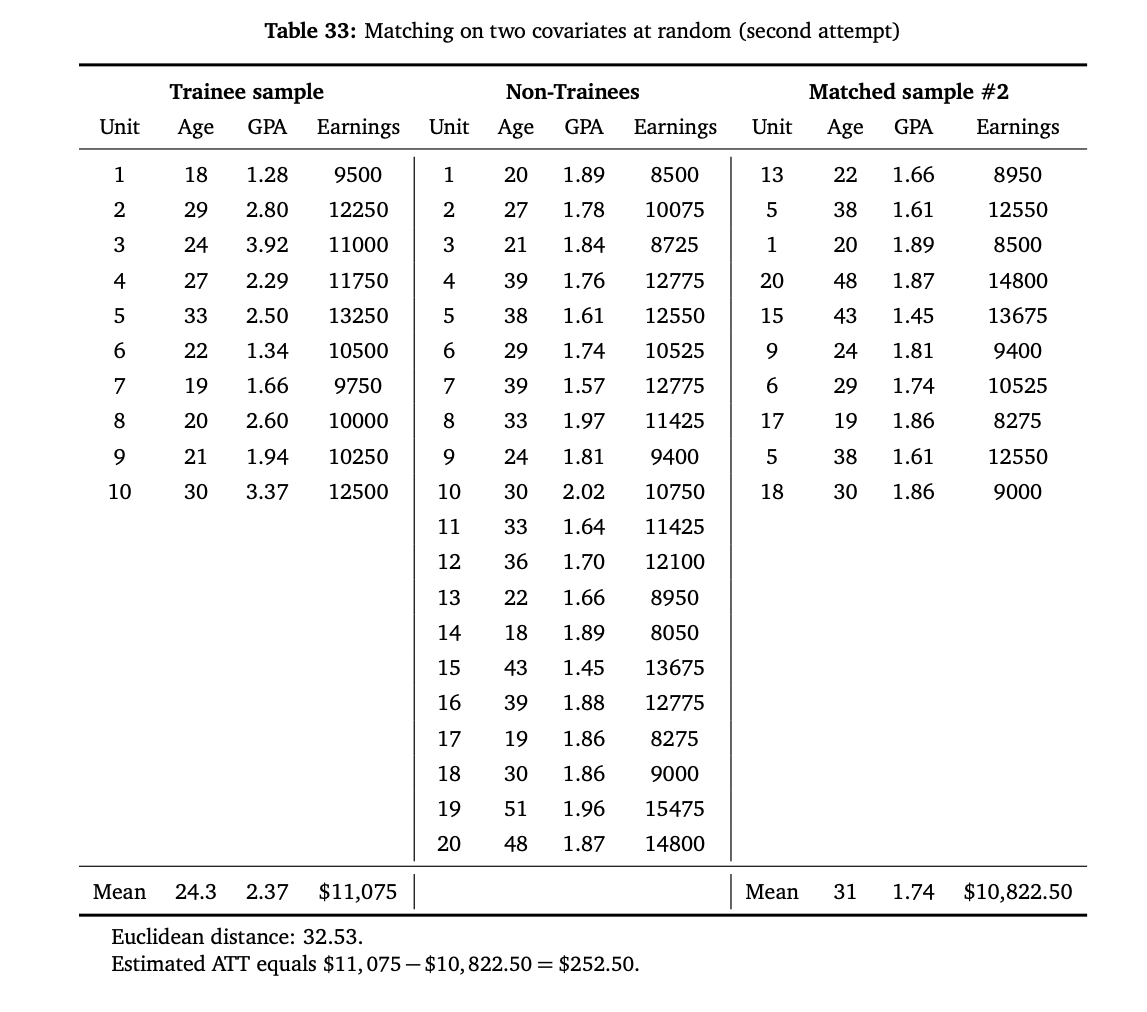
\includegraphics[scale=0.45]{./lecture_includes/inexact_random2}
%\end{figure}

%\end{frame}


\begin{frame}{Minimizing the Euclidean distance}

\begin{itemize}
\item We are minimizing Euclidean distance, and if that is not zero, then there is matching discreprancy
\item And since it is a minimum, any other match will have more matching discreprancies
\item \texttt{Matching} in R and \texttt{teffects} in Stata (not sure in python)
\item Let's look at \texttt{nnmatch1.do} together and see how simple this is
\end{itemize}

\end{frame}




 

%\begin{frame}{Inexact matching by minimizing the Euclidean distance}

%\begin{figure}[!t]\centering
%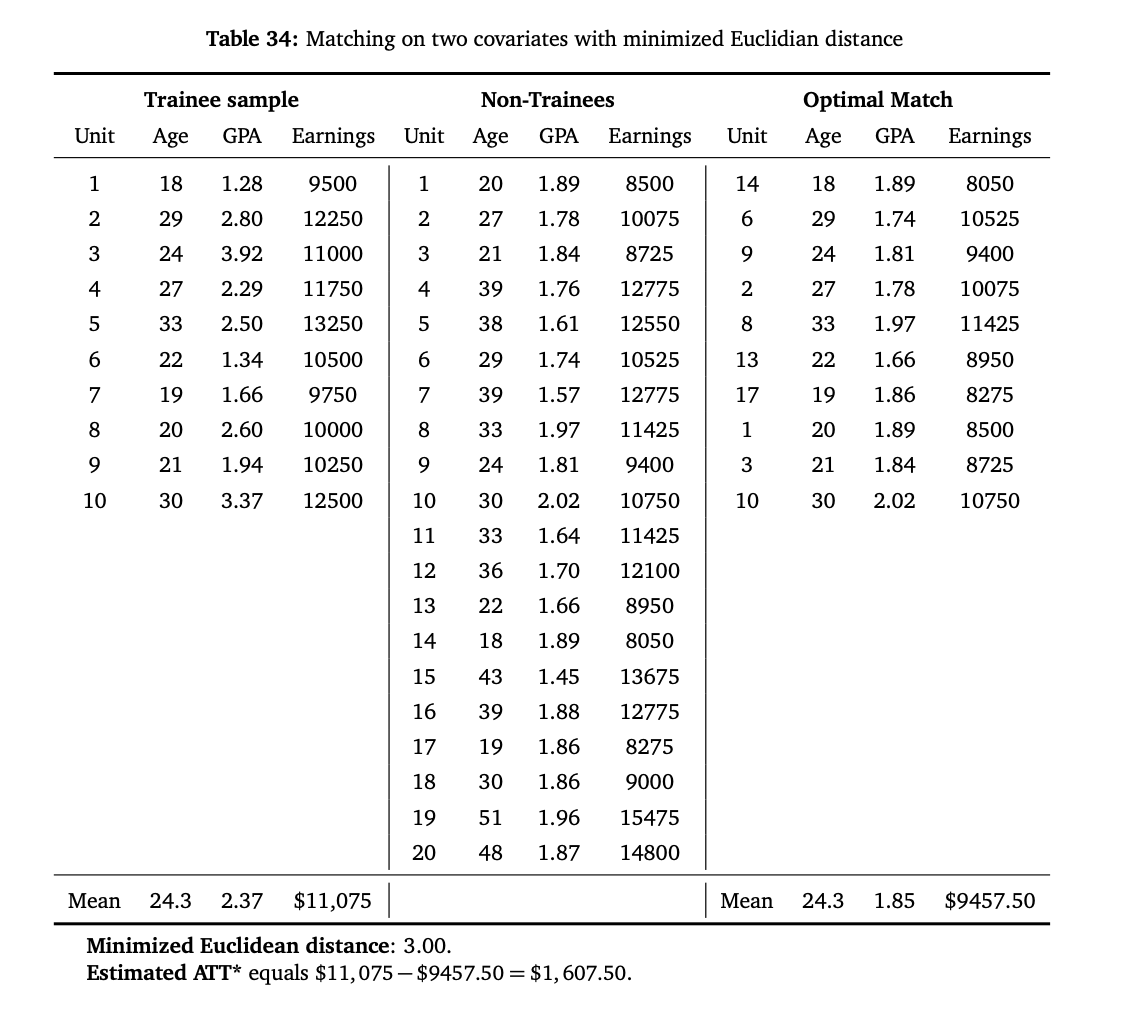
\includegraphics[scale=0.45]{./lecture_includes/inexact_euclidean}
%\end{figure}

%\end{frame}

\begin{frame}{Other distance metrics}

\begin{itemize}
\item Our example treated a one unit difference in age and one unit difference in GPA as the same, but those scales are different and matter a lot
\item The Euclidean distance is not invariant to changes in the scale of the $X$'s.  
\item Alternative distance metrics that \emph{are} invariant to changes in scale are more commonly used 
\item Normalized Euclidean distance and Mahalanobis distance both try to normalize it so that scale doesn't matter
\end{itemize}

\end{frame}


\begin{frame}{Normalized Euclidean distance}

	\begin{block}{Definition: Normalized Euclidean distance}
	  A commonly used distance is the normalized Euclidean distance:$$||X_i-X_j|| = \sqrt{ (X_i-X_j)'\widehat{V}^{-1}(X_i - X_j) }$$ where
		$$\widehat{V}^{-1} = \text{diag}(\widehat{\sigma}_1^2, \widehat{\sigma}_2^2, \dots, \widehat{\sigma}_k^2)$$
	\end{block}
\end{frame}

\begin{frame}{Normalized Euclidean distance}
	\begin{itemize}
	\item Notice that the normalized Euclidean distance is equal to:
		\begin{eqnarray*}
		||X_i - X_j|| = \sqrt{\sum_{n=1}^k \frac{(X_{ni} - X_{nj})^2}{\widehat{\sigma}^2_n}}
		\end{eqnarray*}
	\item Thus, if there are changes in the scale of $X_{ni}$, these changes also affect $\widehat{\sigma}^2_n$, and the normalized Euclidean distance does not change
	\end{itemize}

\end{frame}


\begin{frame}{Mahalanobis distance}
	
	\begin{block}{Definition: Mahalanobis distance}
	The Mahalanobis distance is the scale-invariant distance metric:
		\begin{eqnarray*}
		||X_i-X_j|| = \sqrt{ (X_i-X_j)'\widehat{\Sigma}_X^{-1}(X_i - X_j) }
		\end{eqnarray*}
	where $\widehat{\Sigma}_X$ is the sample variance-covariance matrix of $X$.  
	\end{block}
	
	Let's review them using \texttt{nnmatch2.do}


\end{frame}



\begin{frame}{Matching and the Curse of Dimensionality}
	
\begin{itemize}
\item The larger the dimensions of the conditioning set, the less likely common support holds, and you can't not do it because you need these covariate dimensions to satisfy weak unconfoundedness!
\item This problem is caused by the finite dataset, and it introduces a particular type of selection bias
\item Abadie and Imbens (2011) derived a bias adjustment based on the unconfoundedness assumption and an outcome regression model
\end{itemize}

\end{frame}


\begin{frame}{Deriving the matching bias}
	
  \vspace{-5mm}
  $$
		\widehat{\delta}_{ATT} = \frac{1}{N_T} \sum_{D_i=1} (Y_i - Y_{j(i)}),
  $$
  where each $i$ and $j(i)$ units are matched, $X_i \approx X_{j(i)}$ and $D_{j(i)}=0$. 
	 
  \bigskip
  Define potential outcomes and switching eq.
		\begin{eqnarray*}
      \mu^0(x) &=& E[Y | X=x,D=0] = E[Y^0 | X=x],\\
      \mu^1(x) &=& E[Y | X=x,D=1] = E[Y^1 | X=x],\\
      Y_i &=& \mu^{D_i}(X_i) + \varepsilon_i
		\end{eqnarray*}
\end{frame}

\begin{frame}{Deriving the matching bias}
  Substitute and distribute terms
  \begin{eqnarray*}
    \widehat{\delta}_{ATT} &=& \frac{1}{N_T} \sum_{D_i=1} (Y_i - Y_{j(i)}) \\
    &=& \frac{1}{N_T} \sum_{D_i=1} \left[ (\mu^1(X_i) + \varepsilon_i) - (\mu^0(X_{j(i)}) + \varepsilon_{j(i)}) \right] \\
    &=&  \frac{1}{N_T} \sum_{D_i=1} (\mu^1(X_i) - \mu^0(X_{j(i)})) + \frac{1}{N_T} \sum_{D_i=1}(\varepsilon_i - \varepsilon_{j(i)})
  \end{eqnarray*}
\end{frame}
		

\begin{frame}{Deriving the matching bias}
	
Difference between sample estimate and population parameter is:
		\begin{eqnarray*}
		\widehat{\delta}_{ATT} - \delta_{ATT} &=& \frac{1}{N_T} \sum_{D_i=1} \left( \mu^1(X_i) - \mu^0(X_{j(i)}) - \delta_{ATT}\right) \\
		&+& \frac{1}{N_T} \sum_{D_i=1} (\varepsilon_i - \varepsilon_{j(i)})
		\end{eqnarray*}
Add a zero, algebraic manipulation and simplification:
		\begin{eqnarray*}
		\widehat{\delta}_{ATT} - \delta_{ATT} &=& \frac{1}{N_T} \sum_{D_i=1} \left( \mu^1(X_i) - \textcolor{red}{\mu^0(X_i)} - \delta_{ATT}\right) \\
		&+& \frac{1}{N_T} \sum_{D_i=1} (\varepsilon_i - \varepsilon_{j(i)}) \\
		&+& \frac{1}{N_T} \sum_{D_i=1} \left( \textcolor{red}{\mu^0(X_i)} - \mu^0(X_{j(i)}) \right).
		\end{eqnarray*}
\end{frame}


\begin{frame}{Deriving the matching bias}
	
\begin{itemize}
\item Matching under unconfoundedness is consistent which means this:
$$\widehat{\delta}_{ATT} - \delta_{ATT} \to 0\text{ as N }\to \infty $$.
 \item But in a finite sample, we may never reach the necessary sample size for unbiaseness

$$E[ \sqrt{\frac{1}{N}} (\widehat{\delta}_{ATT} - \delta_{ATT})] = E[ \sqrt{\frac{1}{N}} ( \textcolor{red}{\mu^0(X_i)} - \mu^0(X_{j(i)}) ) | D=1]$$ 

\item When might this happen?  When the dimensions, $k$, are very large (lots of covariates and/or strata dimensions)

\end{itemize}
\end{frame}

\begin{frame}{ Bias is often an issue when we match in many dimensions}

	\begin{itemize}
	\item The difference between $X_i$ and $X_{j(i)}$ converges to zero very slowly 
	\item The selection bias term, $\textcolor{red}{\mu^0(X_i)} - \mu^0(X_{j(i)})$, converges to zero very slowly 
	\item $E[ \sqrt{\frac{1}{N}} (\textcolor{red}{\mu^0(X_i)} - \mu^0(X_{j(i)})) | D=1]$ may not converge to zero and an be very large
	\item And so, $E[ \sqrt{\frac{1}{N}} (\widehat{\delta}_{ATT} - \delta_{ATT})]$ may not converge to zero because the bias of the matching discrepancy is dominating the matching estimator
	\end{itemize}

\end{frame}

\begin{frame}{Solutions to matching bias problem}
	
The bias of the matching estimator is caused by large matching discrepancies $||X_i - X_{j(i)}||$ which is virtually guaranteed by the curse of dimensionality.  However:
	\begin{enumerate}
	\item But the matching discrepancies are observed. We can always check in the data how well we're matching the covariates.

	\item For $\widehat{\delta}_{ATT}$ we can sometimes make the matching discrepancies small by using a large reservoir of untreated units to select the matches (that is, by making $N_C$ large).

  \item If the matching discrepancies are large, so we are worried about potential biases, we can apply bias correction techniques

	\end{enumerate}
\end{frame}

 
\begin{frame}{Matching with bias correction}
	
	\begin{itemize}
	\item Each treated observation contributes$$\textcolor{red}{\mu^0(X_i)} - \mu^0(X_{j(i)})$$to the bias.
	\item Bias-corrected (BC) matching:
		\begin{eqnarray*}
		\widehat{\delta}_{ATT}^{BC} = \frac{1}{N_T} \sum_{D_i=1} \left[ (Y_i - Y_{j(i)}) - ( \widehat{\mu^0}(X_i) - \widehat{\mu^0}(X_{j(i)}) ) \right]
		\end{eqnarray*}where $\widehat{\mu^0}(X)$ is an estimate of $E[Y|X=x,D=0]$.  For example using OLS but other maybe too (neural nets?).  
	\item Under some conditions, the bias correction eliminates the bias of the matching estimator without affecting the estimator's variance.
	\end{itemize}
\end{frame}

\begin{frame}{Intuition}

\begin{itemize}
\item Under unconfoundedness, we know that $$\textcolor{red}{E[Y^0|D=1, X=x]} = E[Y^0|D=0, X=x]$$
\item This implies that whatever the relationship is between $Y^0$ and $X$ in the control group, it's the same in the treatment group, even though we cannot observe $Y^0$ in the treatment group
\item We will therefore fit a regression of $Y^0$ onto $X$ in the $D=0$ group only and use that to predict $\widehat{Y^0}$ in both groups
\end{itemize}

\end{frame}

\begin{frame}{Bias correction steps}

\begin{figure}[!t]\centering
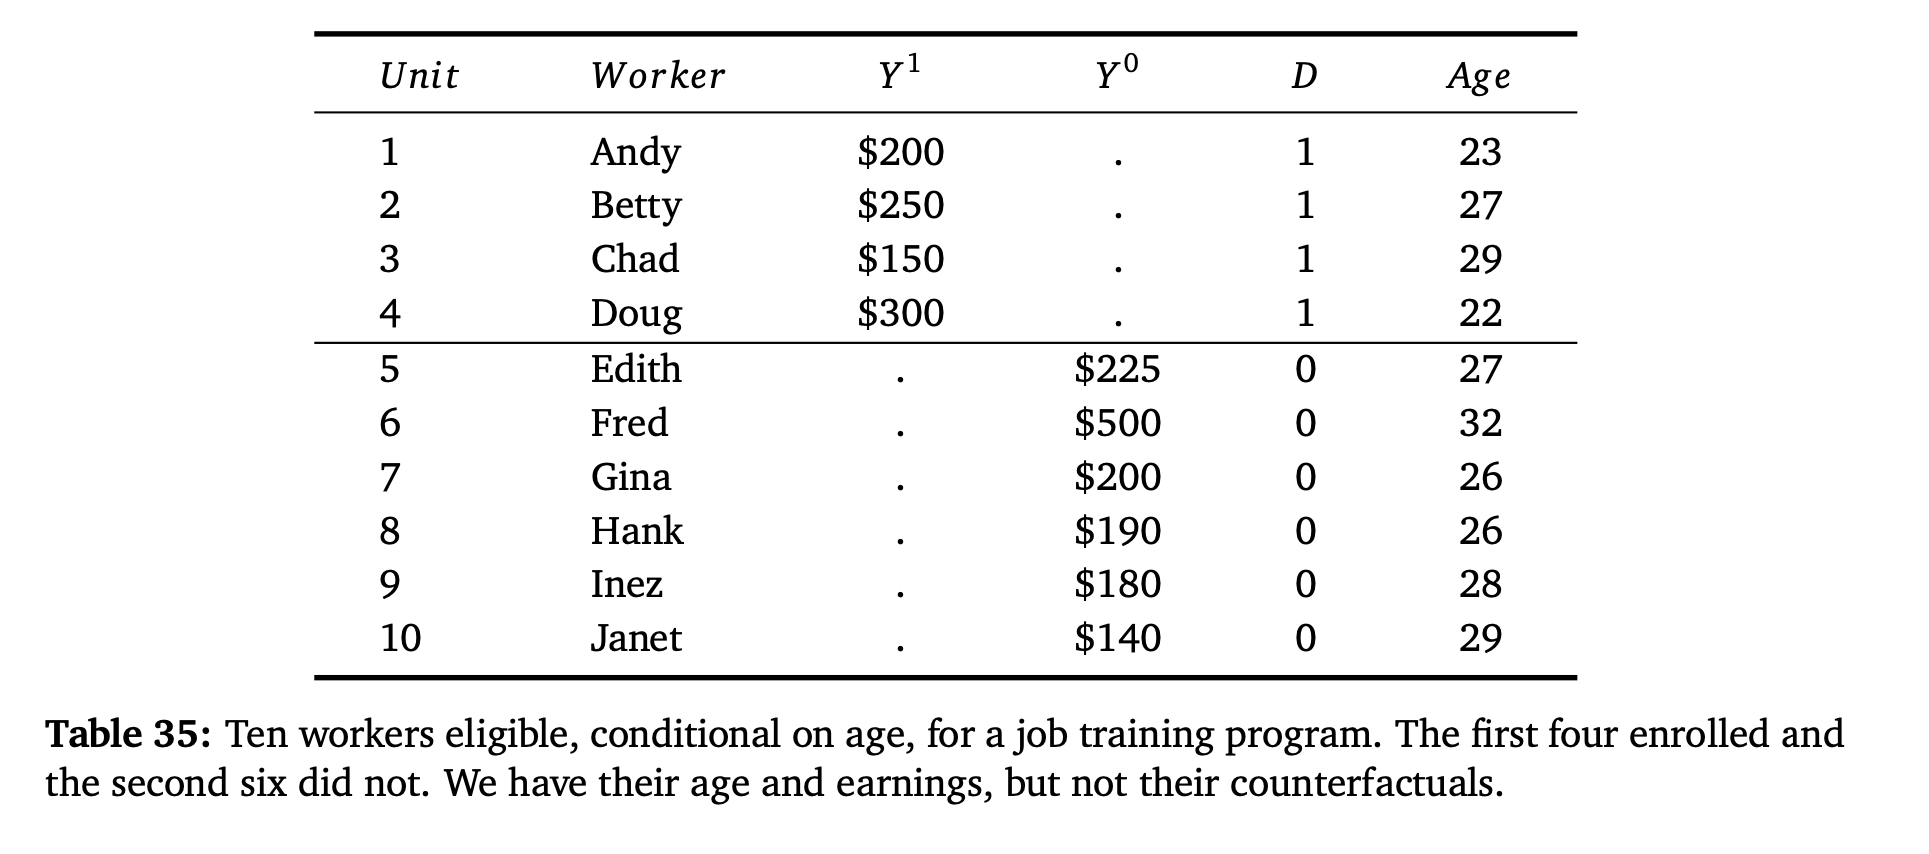
\includegraphics[scale=0.35]{./lecture_includes/nnmatch_bc1}
\end{figure}

\end{frame}



\begin{frame}{Bias correction steps}

\begin{figure}[!t]\centering
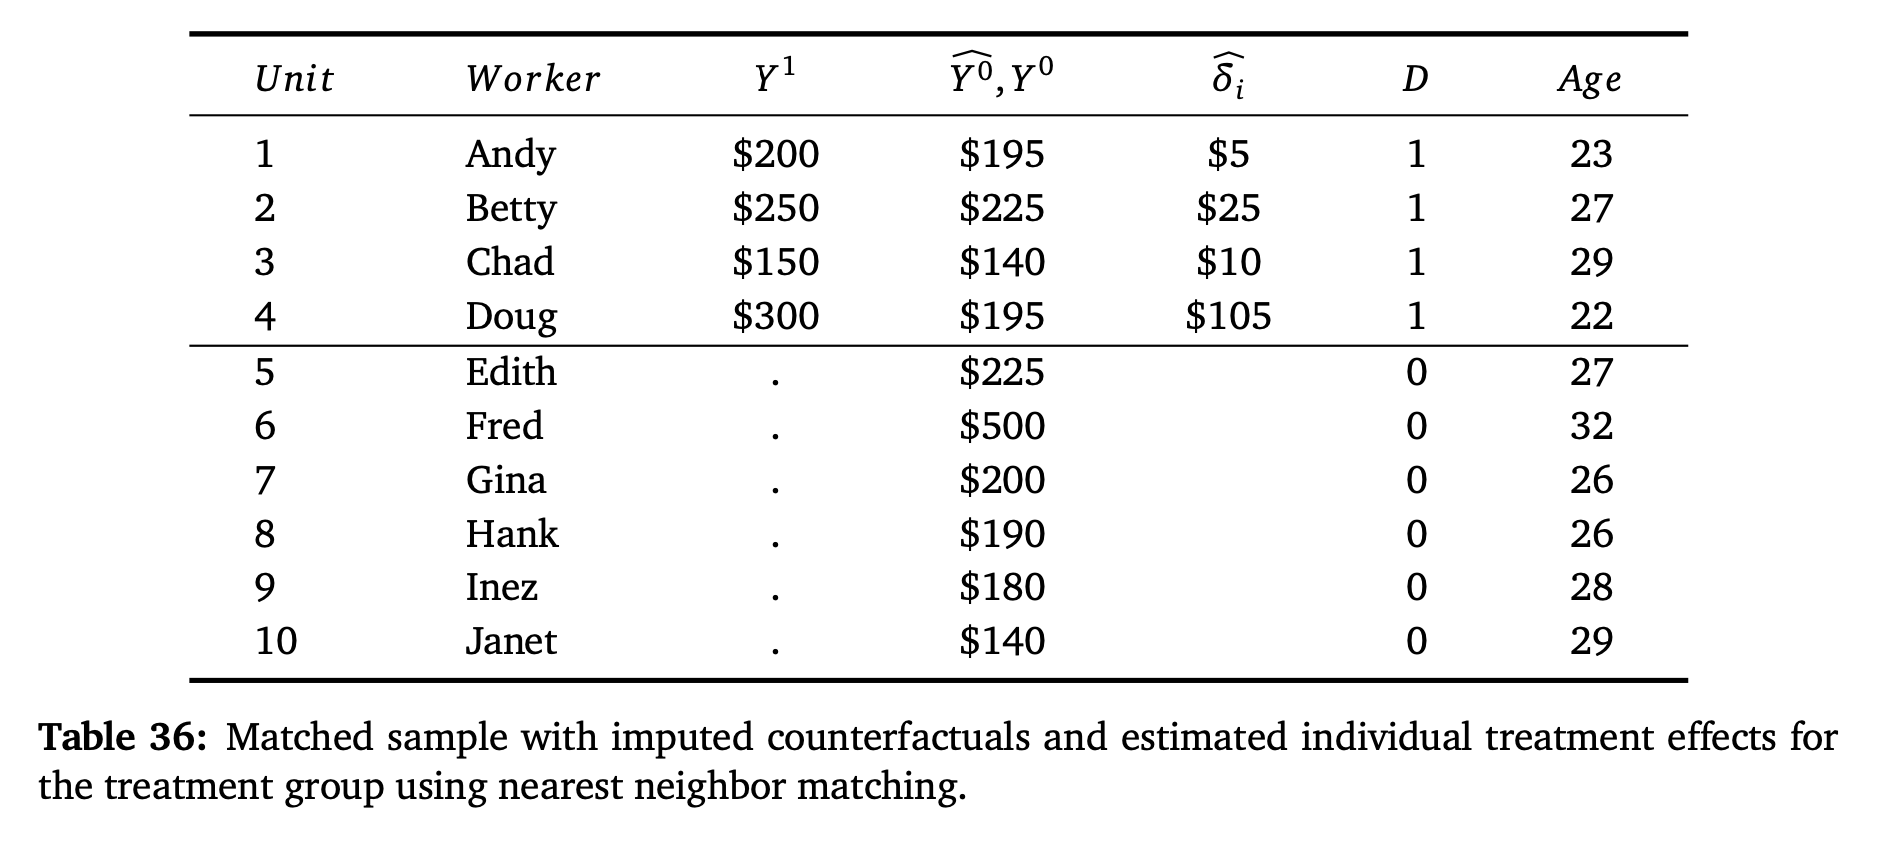
\includegraphics[scale=0.35]{./lecture_includes/nnmatch_bc2}
\end{figure}

\end{frame}


\begin{frame}{Steps}

\begin{enumerate}
\item[1.  ]Regress $Y$ on $X$ with OLS except only use the \emph{matched} sample of control group units:
\begin{equation}
Y^0_j = \alpha + \beta X_j + \varepsilon_j \nonumber
\end{equation}where $j$ are the units for which $D_j=0$.  Examine the code for this in \texttt{nnmatch_bc1.do} and \texttt{nnmatch_bc2.do}.
\end{enumerate}

\end{frame}

\begin{frame}{Steps}

\begin{enumerate}
\item[2. ] Use the fitted values $\widehat{\alpha}$ and $\widehat{\beta}$ to predict $\widehat{\mu}^0(X)$ for both the $i$ and the matched $j(i)$ units:
\begin{eqnarray}
\widehat{\mu}^0_i &=& \widehat{\alpha} + \widehat{\beta} X_i \nonumber \\
\widehat{\mu}^0_{j(i)} &=& \widehat{\alpha} + \widehat{\beta} X_{j(i)} \nonumber
\end{eqnarray}
\end{enumerate}

\end{frame}


\begin{frame}{Steps}

\begin{enumerate}
\item[3. ] Subtract $ \widehat{\mu}_i^0(X_i) - \widehat{\mu}_{j(i)}^0(X_{j(i)})$, our estimate of the selection bias caused by matching discrepancies, from the sample estimate of the $ATT$: $$\widehat{\delta}_{ATT}^{BC} = \dfrac{1}{N_T} \sum_{D_i=1} \bigg [ (Y_i - Y_{j(i)}) - \Big(\widehat{\mu}^0(X_i) - \widehat{\mu}^0(X_{j(i)})\Big) \bigg ]$$
\end{enumerate}

\end{frame}


\begin{frame}{Steps}

\begin{enumerate}
\item[4. ] Estimate Abadie-Imbens robust standard error (Abadie and Imbens 2006; 2008; 2011)
\end{enumerate}

Let's review all of this \texttt{nnmatch_bc1.do} and \texttt{nnmatch_bc2.do}

\end{frame}






\begin{frame}{Matching bias: Implications for practice}
	
\emph{Matching} bias arises because of the effect of large matching discrepancies on $\mu^0(X_i) - \mu^0(X_{j(i)})$ due to a lack of common support. To minimize matching discrepancies:
	\begin{enumerate}
	\item Use a small $M$ (e.g., $M=1$). Larger values of $M$ produce large matching discrepancies.
	\item Use matching with replacement.  Because matching with replacement can use untreated units as a match more than once, matching with replacement produces smaller matching discrepancies than matching without replacement.
	\item Try to match covariates with a large effect on $\mu^0(\cdot)$ particularly well.
	\end{enumerate}
\end{frame}

\begin{frame}{Bias Correction}

\begin{itemize}

\item Consider \texttt{matching_biasadj.do} that examines three models:
	\begin{enumerate}
	\item Underfit model with and without bias correction
	\item Correctly specified model with and without bias correction
	\item Overfit model with and without bias correction
	\end{enumerate}
\item Overfit model included cubic even though correct model was quadratic
\end{itemize}

\end{frame}


\begin{frame}{Simulation}
\begin{figure}[htbp]
    \centering
    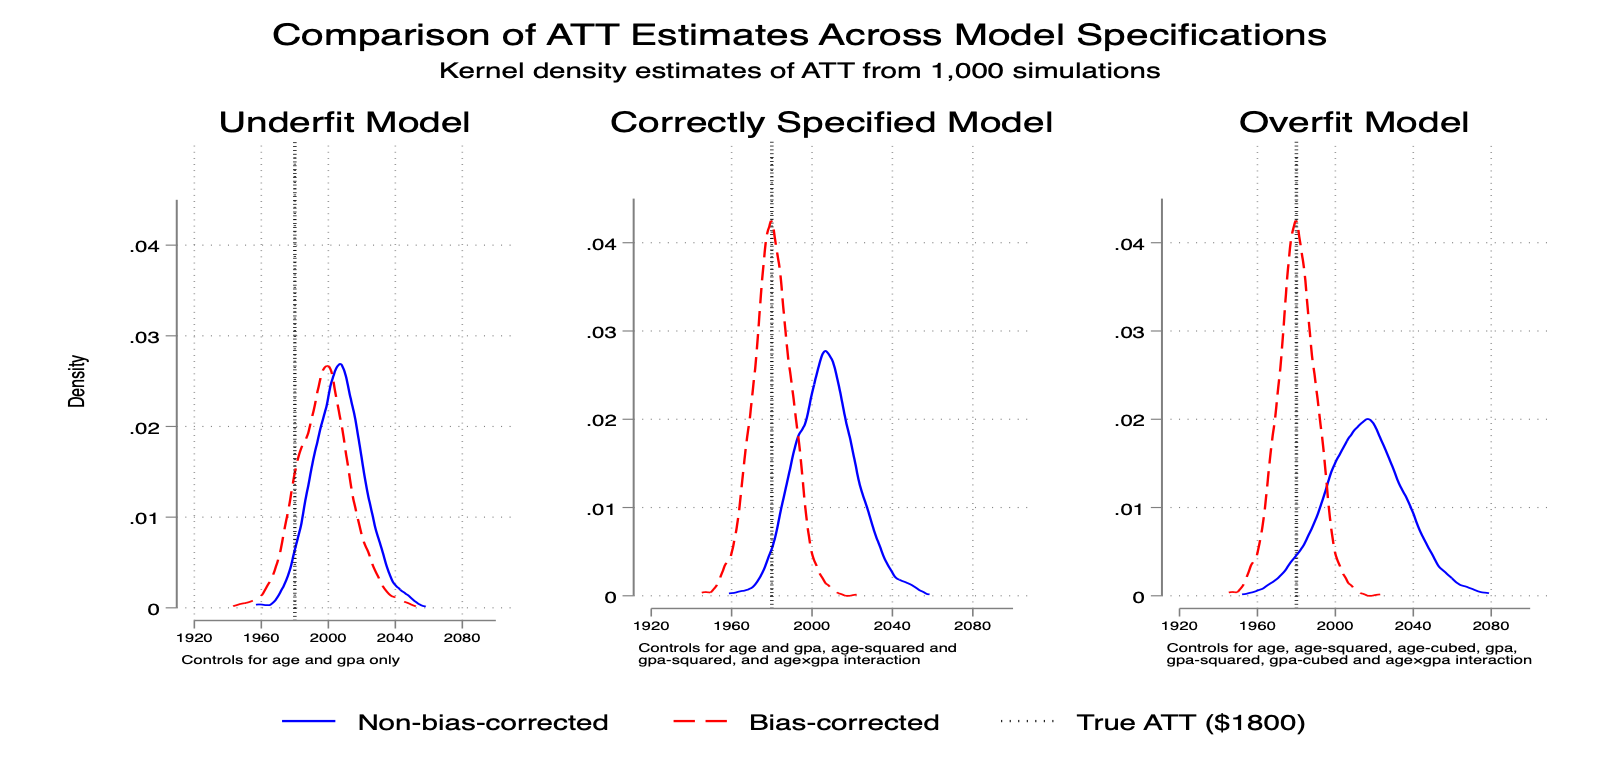
\includegraphics[width=0.9\textwidth, height=0.65\textheight]{./lecture_includes/att_estimates_comparison.png}
    \label{fig:nnmatch_estimates1}
\end{figure}

\end{frame}


\begin{frame}{Large sample distribution for matching estimators}
	
	\begin{itemize}
	\item Cannot use the bootstrap, so Abadie and Imbens derived the variance (Abadie and Imbens 2008)
	\item Matching estimators have a Normal distribution in large samples (provided the bias is small):
		\begin{eqnarray*}
		\sqrt{N_T} (\widehat{\delta}_{ATT} - \delta_{ATT}) \xrightarrow{d} N(0,\sigma^2_{ATT})
		\end{eqnarray*}
	\item For matching without replacement, the ``usual'' variance estimator:
		\begin{eqnarray*}
		\widehat{\sigma}^2_{ATT} = \frac{1}{N_T} \sum_{D_i=1} \left( Y_i - \frac{1}{M} \sum_{m=1}^M Y_{j_m(i)} - \widehat{\delta}_{ATT} \right)^2,
		\end{eqnarray*}is valid.
	\end{itemize}
\end{frame}

\begin{frame}{Large sample distribution for matching estimators}
	
	\begin{itemize}
	\item For matching with replacement:
		\begin{eqnarray*}
		\widehat{\sigma}^2_{ATT} &=& \frac{1}{N_T} \sum_{D_i=1} \left( Y_i - \frac{1}{M} \sum_{m=1}^M Y_{j_m(i)} - \widehat{\delta}_{ATT} \right)^2 \\
		&+& \frac{1}{N_T} \sum_{D_i=0} \left( \frac{K_i(K_i-1)}{M^2} \right) \widehat{var}(\varepsilon | X_i,D_i=0)
		\end{eqnarray*}where $K_i$ is the number of times observation $i$ is used as a match.
	\item $\widehat{var}(Y_i | X_i,D_i=0)$ can be estimated also by matching.  For example, take two observations with $D_i=D_j=0$ and $X_i \approx X_j$, then
		\begin{eqnarray*}
		\widehat{var}(Y_i | X_i,D_i=0) = \frac{(Y_i-Y_j)^2}{2}
		\end{eqnarray*}is an unbiased estimator of $\widehat{var}(\varepsilon_i | X_i,D_i=0))$
	\end{itemize}
\end{frame}

\begin{frame}{Example}

Let's now review the syntax in Stata.  It's called \texttt{matching.do} and is in /Labs/Matching 

\bigskip

\url{https://github.com/Mixtape-Sessions/Causal-Inference-1/tree/main/Lab/Matching}

\end{frame}


\subsection{Propensity scores}


\begin{frame}{Propensity scores}

\begin{itemize}
\item Alternative to the distance minimization method is to use something called the "propensity score" to summarize all of the covariates into a single scalar and then weight or match on it 
\item Propensity score was introduced by Rosenbaum and Rubin (1983) and has become extremely influential in causal inference
\end{itemize}



\end{frame}

\begin{frame}{Propensity score theorem}

\footnotesize
``We are interested in estimating the average effect of a binary treatment on a scaler outcome.  If assignment to the treatment is exogenous or unconfounded, that is, independent of the potential outcomes given covariates, biases associated with simple treatment-control average comparisons can be removed by adjusted for differences in the covariates.  Rosenbaum and Rubin (1983) show that adjusting solely for differences between treated and control units in the propensity score removes all biases associated with differences in covariates.'' -- Hirano, Imbens and Ridder (2003, Econometrica)

\end{frame}





\begin{frame}{Formal Definition}
	
	\begin{block}{Definition of Propensity score}
	A propensity score is a person (or "unit") specific probability bounded between 0 and 1 measuring the probability of treatment assignment given a collection of variables: $p(X)=Pr(D=1 | X)$
	\end{block}
	

\end{frame}


\begin{frame}{Propensity score theorem}
	
	\begin{block}{Propensity score theorem}
	If $(Y^1,Y^0)\independent{D}|X$ (full unconfoundedness), then $(Y^1,Y^0)\independent{D} | \rho(X)$ where $\rho(X)=Pr(D=1|X)$, the propensity score
	\end{block}
	
	\begin{itemize}
	\item Conditioning on the propensity score is enough to have independence between $D$ and $(Y^1,Y^0)$ (Rosenbaum and Rubin 1983)
	\item With full unconfoundedness, you can estimate the ATE, but you can estimate the ATT with weaker assumptions (independence with respect to $(Y^0)\independent{D} | \rho(X)$)
	\item But remember -- propensity scores don't solve unconfoundedness; if you don't have it with respect to $K$ dimensions of $X$, you won't have it when you collapse it to the propensity score
	\end{itemize}
\end{frame}

\begin{frame}{True vs Estimating Propensity Score}


\begin{itemize}
\item Outside the randomized experiment, we don't know the ``true propensity score''
	\begin{itemize}
	\item We use DAGs or hunches to select covariates, careful not to include outcomes or colliders
	\item But we still won't know the functional form (i.e., logit, probit, polynomials, interactions)
	\end{itemize}
\item Often then people will use higher order terms and interactions to provide flexibility but it does technically have misspecification biases
\item This is an area most likely where machine learning could greatly enhance the estimation (take your pick)
\end{itemize}

\end{frame}




\begin{frame}{Step 1: Pick your parameter ATE vs ATT vs ATU}

\begin{itemize}
	\item Which population are you studying?  Only those who were discriminated against?  That's the ATT
	\item Do you want to imagine ``what if blacks and whites were both discriminated against?'' That's the ATE
	\item The more you can focus on one particular causal parameter, the easier and more justified it gets as it weakens both assumptions
\end{itemize}

\end{frame}


\begin{frame}{Step 2: Estimate the propensity score}

		\begin{itemize}
		\item Estimate the conditional probability of treatment using probit or logit model (or ML) $$Pr(D_i=1|X_i) = F(\beta X_i)$$
			\item Note: don't use OLS because while it will get the mean right, it will not get correct values in the tails because of its linear projections
			\item OLS will give propensity scores outside the [0,1] bounds and probabilities cannot be negative or greater then one
		\end{itemize}
\end{frame}

\begin{frame}{Step 2: Estimate the propensity score}

		\begin{itemize}
		\item Use the estimated coefficients to predict the propensity score for each unit $i$$$\widehat{\rho}_i(X_i) = \widehat{\beta} X_i$$
		\item Note that each unit $i$ now has a predicted probability of treatment given the values of their covariates relative to everyone else's 
		\end{itemize}
\end{frame}



\begin{frame}{Step 2: Estimate the propensity score}

\begin{itemize}
\item Think of the propensity score as a frequentist concept of probability
\item ``If I drew someone from the sample with these characteristics, then how many of those are in the treatment group divided by the total with those characteristics'' 
\item Or for each dimension of $X$, a ratio of $\frac{N_T}{(N_T + N_C)}$

\end{itemize}

\end{frame}


\begin{frame}{Propensity score as dimension reduction}
	
	\begin{itemize}

	\item Rubin (1977) and Rosenbaum and Rubin (1983) developed the propensity score method
	\item They show that if treatment is independent of potential outcomes conditional on $K$ covariates, then it will be independent of potential outcomes conditional on propensity score 
	\item Main value of the propensity score is dimension reduction  to reduce $K$ covariates into a single scalar without loss of information
	\item Variety of ways to incorporate the propensity score -- stratification, weighting and matching
	\end{itemize}
	
\end{frame}


\begin{frame}{Investigating overlap}

\begin{itemize}

\item Once you obtain the propensity score, you can use it for estimation, but you can also use it for evaluating covariate balance
\item It's an easy way to do it with histograms, and since the propensity score theorem holds for the dimensions of $X$, there's no loss of generality in investigating overlap that way versus one by one 
\item Remember: you need common support, not on $X$ individual covariates alone, but within the $K$ dimensions, so investigating with the propensity score is easier to do

\end{itemize}

\end{frame}



\begin{frame}{Covariate 1  histograms}

  \begin{figure}
    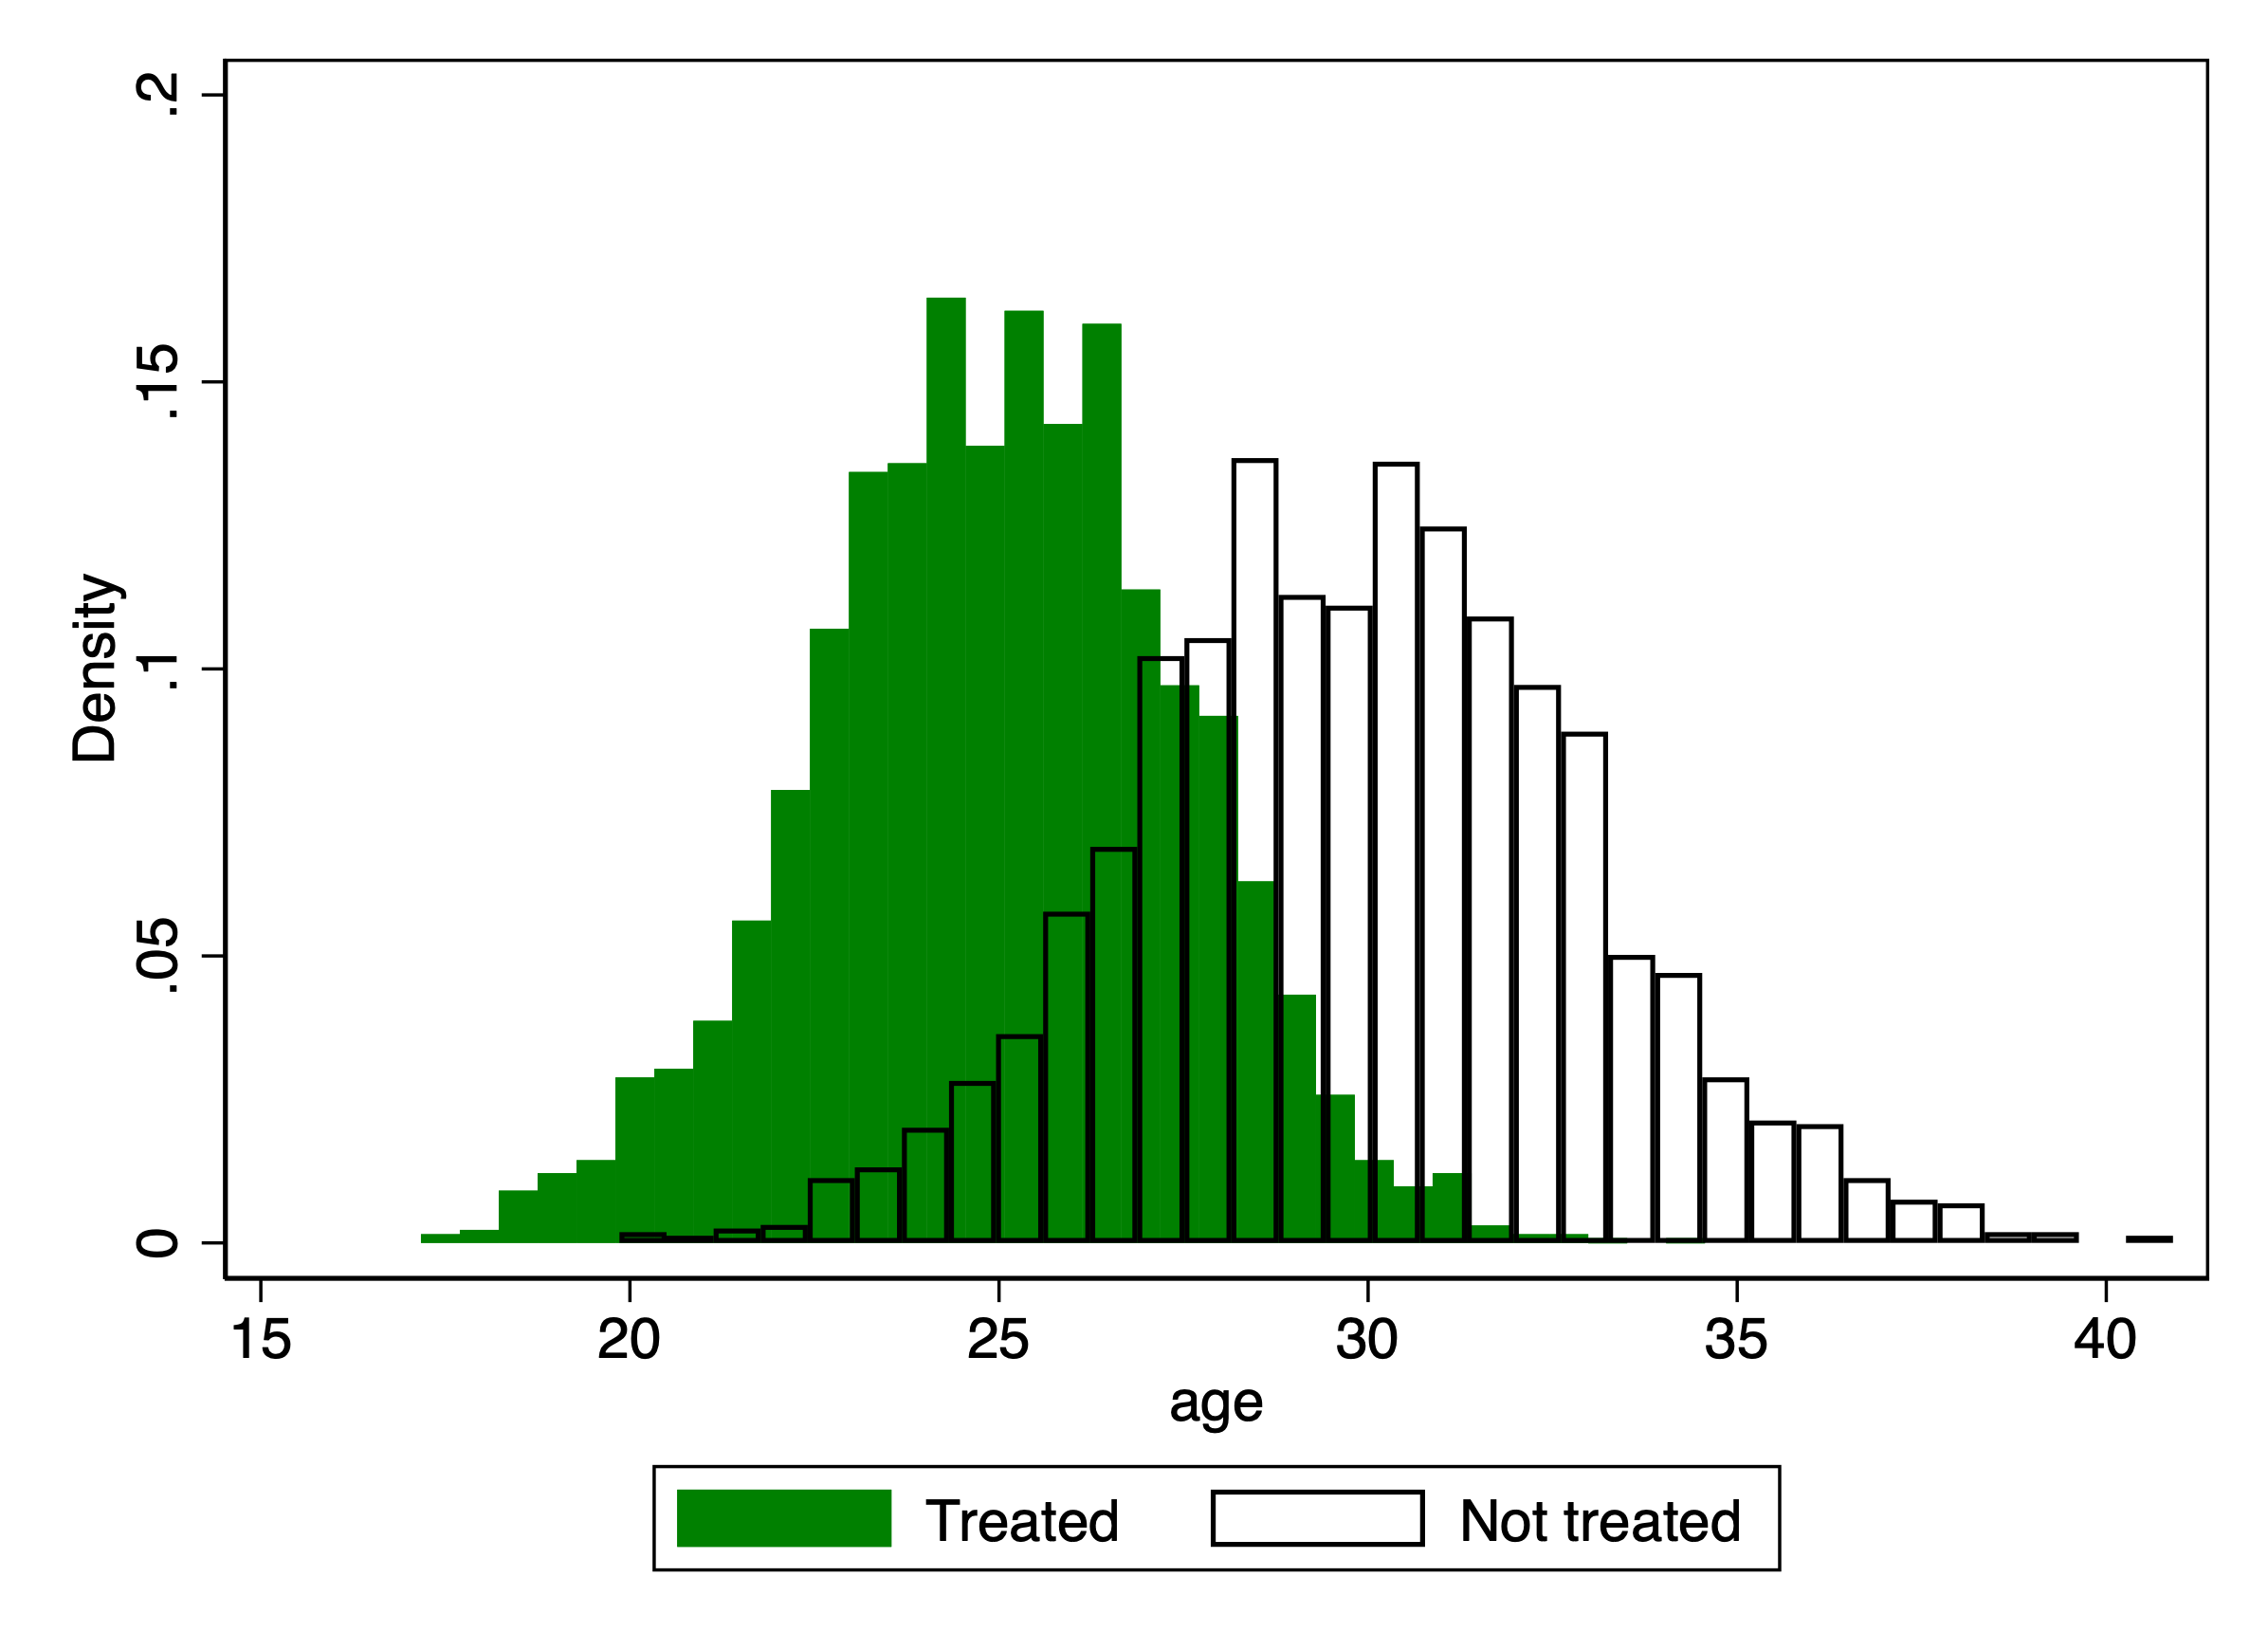
\includegraphics[scale=0.25]{./lecture_includes/age_histogram}
  \end{figure}
  
\end{frame}

\begin{frame}{Covariate 2  histograms}

  \begin{figure}
    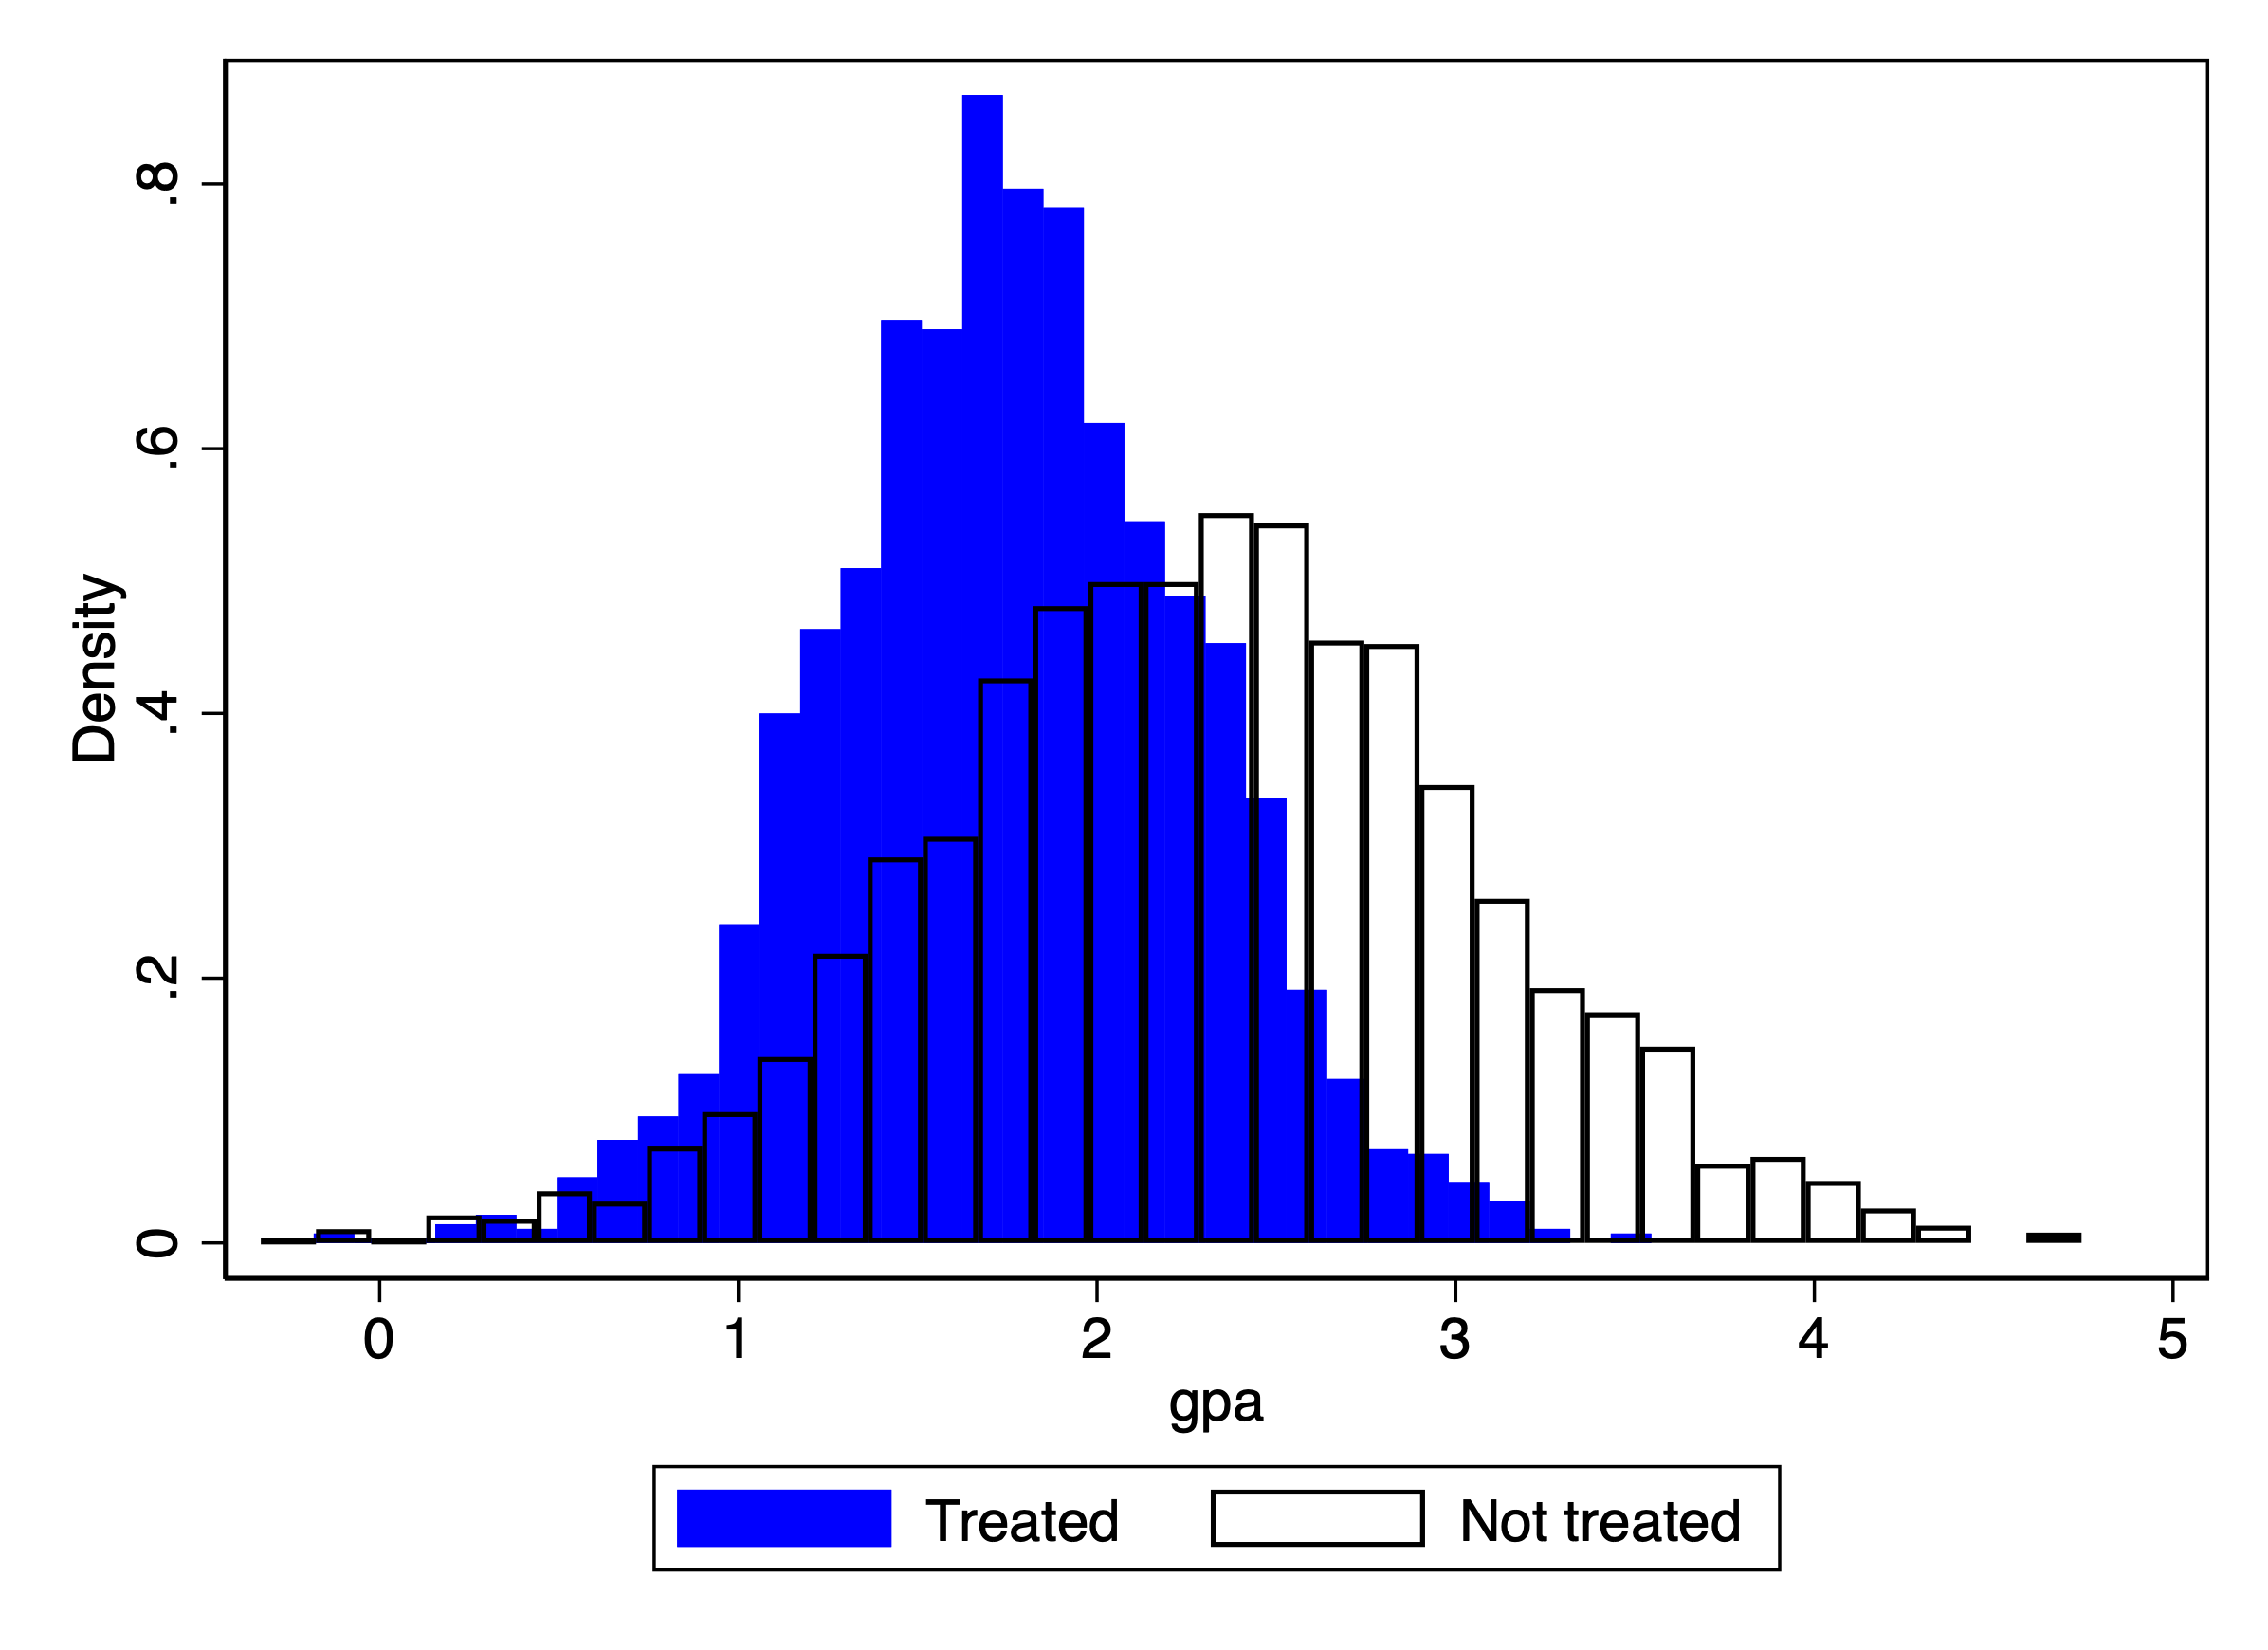
\includegraphics[scale=0.25]{./lecture_includes/gpa_histogram}
  \end{figure}
  
\end{frame}

\begin{frame}{Propensity scores}

  \begin{figure}
    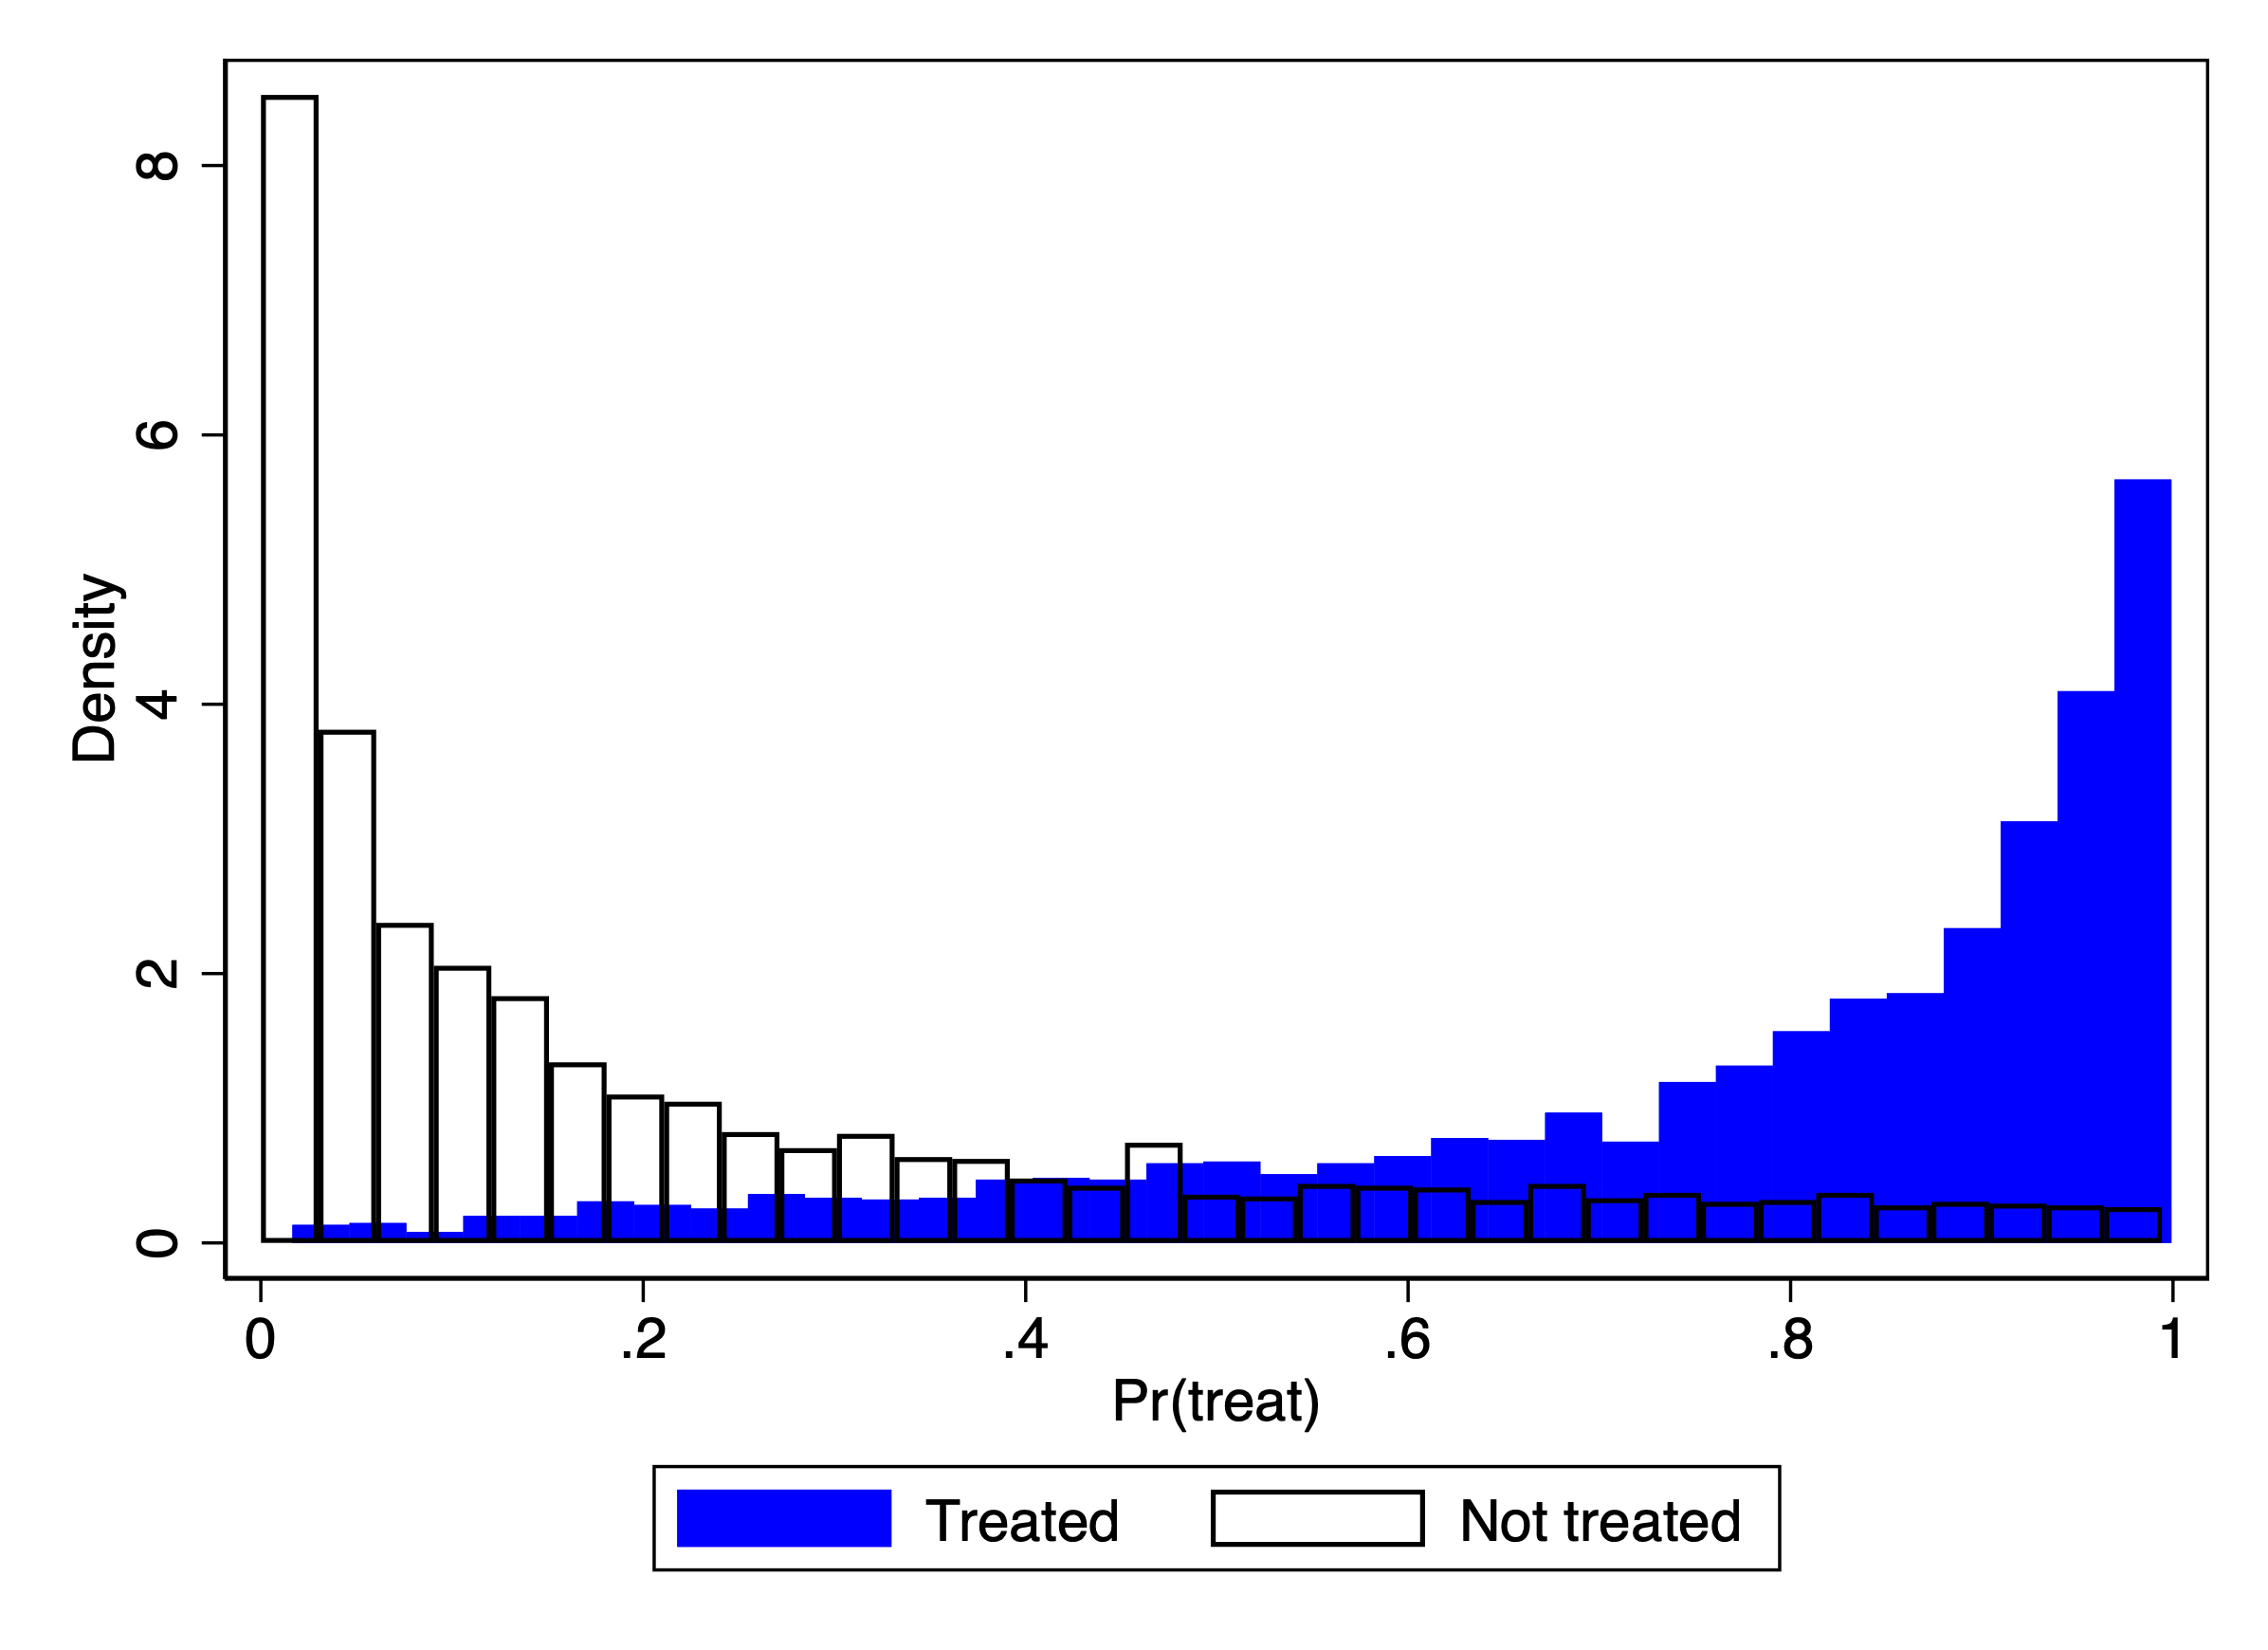
\includegraphics[scale=0.25]{./lecture_includes/pscore_histogram}
  \end{figure}
  
\end{frame}




\begin{frame}{Navigating the vastness of estimation}

\begin{itemize}
\item Estimators abound and can be a little bewildering so to summarize them:
	\begin{enumerate}
	\item Match units from one group to another using the propensity score (with various rules for finding how close to be)
	\item Weighting by the inverse propensity score
	\end{enumerate}
\item Variety of techniques to derive standard errors from parametric methods to bootstrapping
\item Can even introduce ``doubly robust'' methods to deal with matching bias like we did with nearest neighbor bias correction
\item But all these estimators assume unconfoundedness, so really it's all about addressing the lack of overlap; that's the only bias that exists when you have unconfoundedness remember
\end{itemize}

\end{frame}




\begin{frame}{Step 3a: Estimation  with matching}

\begin{itemize}
	
	\item Most common method is to use matching
	\item Matching finds a unit in the comparison group with a similar $\widehat{\rho}_i(X)$ to service as counterfactual for the unit
	\item For the ATE, you'll need matches on both side; for the ATT, you'll need matches for the treatment group among controls
	\item Lack of overlap creates issues for matching which we'll note later
	
\end{itemize}

\end{frame}


\begin{frame}{Step 3a: Estimation with stratification}

\begin{itemize}
	
	\item Rare to see this done anymore, though it was one of the methods that Dehejia and Wahba (2002) tried
	\item Stratification is a kind of weighting method similar to Cochran's subclassification method where weights are group shares within certain ranges of the propensity score
	\item Four steps to doing this; I'll review again later, but let me briefly do it now
	
\end{itemize}

\end{frame}


\begin{frame}{Step 3a: Estimation with stratification}

\begin{enumerate}
	\item First, split the sample by ranges on the propensity score until you find covariate balance within each range
	\item Next calculate weights for each region depend on the causal parameter you're seeking:
		\begin{itemize}
		\item ATE: number of units in that region divided by total units in sample ;
		\item ATT: number of treated units in that region divided by the number of treated units in the sample
		\item ATU: number of control units in that region divided by the number of control units in the sample
		\end{itemize}
	\item Calculate simple difference in mean outcomes (i.e., without controls) for each propensity score region (Step 1)
	\item Then take weighted average using weights from step 2 and difference in means from step 3
\end{enumerate}

\end{frame}




\begin{frame}{Step 3b: Early weighting methods}

\begin{itemize} 
\item Heckman, Ichimura, and Todd (1997, 1998) and Heckman, Ichimura, Smith,
and Todd (1998) focus on the ATT
\item Estimators based on local linear regressions of the outcome on treatment status and either covariates or the propensity score. 
\item They conclude that in general there is no clear ranking of their estimators 
\item Under some conditions the estimator based on adjustment for all covariates is superior to the estimator based on adjustment for the propensity score, \item Under other conditions the second estimator is to be preferred and lack of knowledge of the propensity score does not alter this conclusion
\end{itemize}

\end{frame}

	

\begin{frame}{Step 3b: IPW by Hirano, Imbens and Ridder}

\begin{itemize} 
\item Hirano, Imbens and Ridder (2003, Econometrica) considers estimation of the ATT
\item Focus is on the efficient estimation and they show that while weighting on the inverse of the true propensity score is not an efficient estimator, paradoxically weighting each observation by the \emph{inverse} of a nonparametric estimator of the propensity score is
\end{itemize}

\end{frame}


\begin{frame}{Step 3b: Estimation with inverse probability weighting}

\begin{itemize}
	\item IPW uses the estimated propensity score to reweight the outcomes for which there are several historical methods for doing so
	\item IPW is non-parametric -- you are just taking averages and multiplying by the inverse of the propensity score weights depending on which parameter you want to estimate
	\item There are fewer implementation choices than in matching (i.e., no choice over distance, number of neighbors)
	\item There are bias adjustment methods called double robust where you combine imputing counterfactuals with weighting by the propensity score
\end{itemize}

\end{frame}
	


	

\begin{frame}{Step 3b: Estimation of ATT with IPW}
	
		\begin{block}{Estimating ATT with IPW}
	Given $Y^0 \independent{D}|X$ and weak common support, then
		\begin{eqnarray*}
		\delta_{ATT}&=&E[Y^1-Y^0|D=1] \\
		&=& \frac{1}{Pr(D=1)} \cdot  E \left[ Y \cdot \frac{D-\rho(X)}{1-\rho(X)} \right]
		\end{eqnarray*}
	\end{block}Notice that when $D=1$, the outcome is not weighted, but when $D=0$ it is. You're missing the $Y^0$ for the treatment, not $Y^1$ so you the treatment group $Y$ values alone and weight ``up'' or ``down'' the comparison groups by their propensity scores

\end{frame}


\begin{frame}{Step 4: Standard Errors}
	
		
Standard errors can be constructed a few different ways:
	\begin{itemize}
	\item We need to adjust the standard errors for first-step estimation of $\rho(X)$
		\begin{itemize}
		\item Parameteric first step: Newey and McFadden (1994)
		\item Non-parametric first step: Newey (1994)
		\end{itemize}
	\item IPW is a smooth estimator which means the bootstrap is valid for inference  (Adudumilli 2018 and Bodory et al. 2020) 
	\end{itemize}
\end{frame}


\begin{frame}{Check for common support using histograms}

\begin{itemize}

\item Assessing whether there are units it both groups for whichever parameter you're focused on is simple with propensity score as shown earlier using histograms of the propensity score for treated and control
\item Crump, et al. (2009) suggest keeping propensity scores within the interval [0.1,0.9] (``trimming'') but any trimming will drop units and dropping units means we are not estimating the ATT
\item We are rather estimating the average treatment effect for the remaining units satisfying overlap (ATTO or something)
\item Let's look at a picture again just to remind ourselves (and we can look at \texttt{matching.do} again)

\end{itemize}

\end{frame}

\begin{frame}{Assessing overlap}

\begin{figure}[!t]\centering
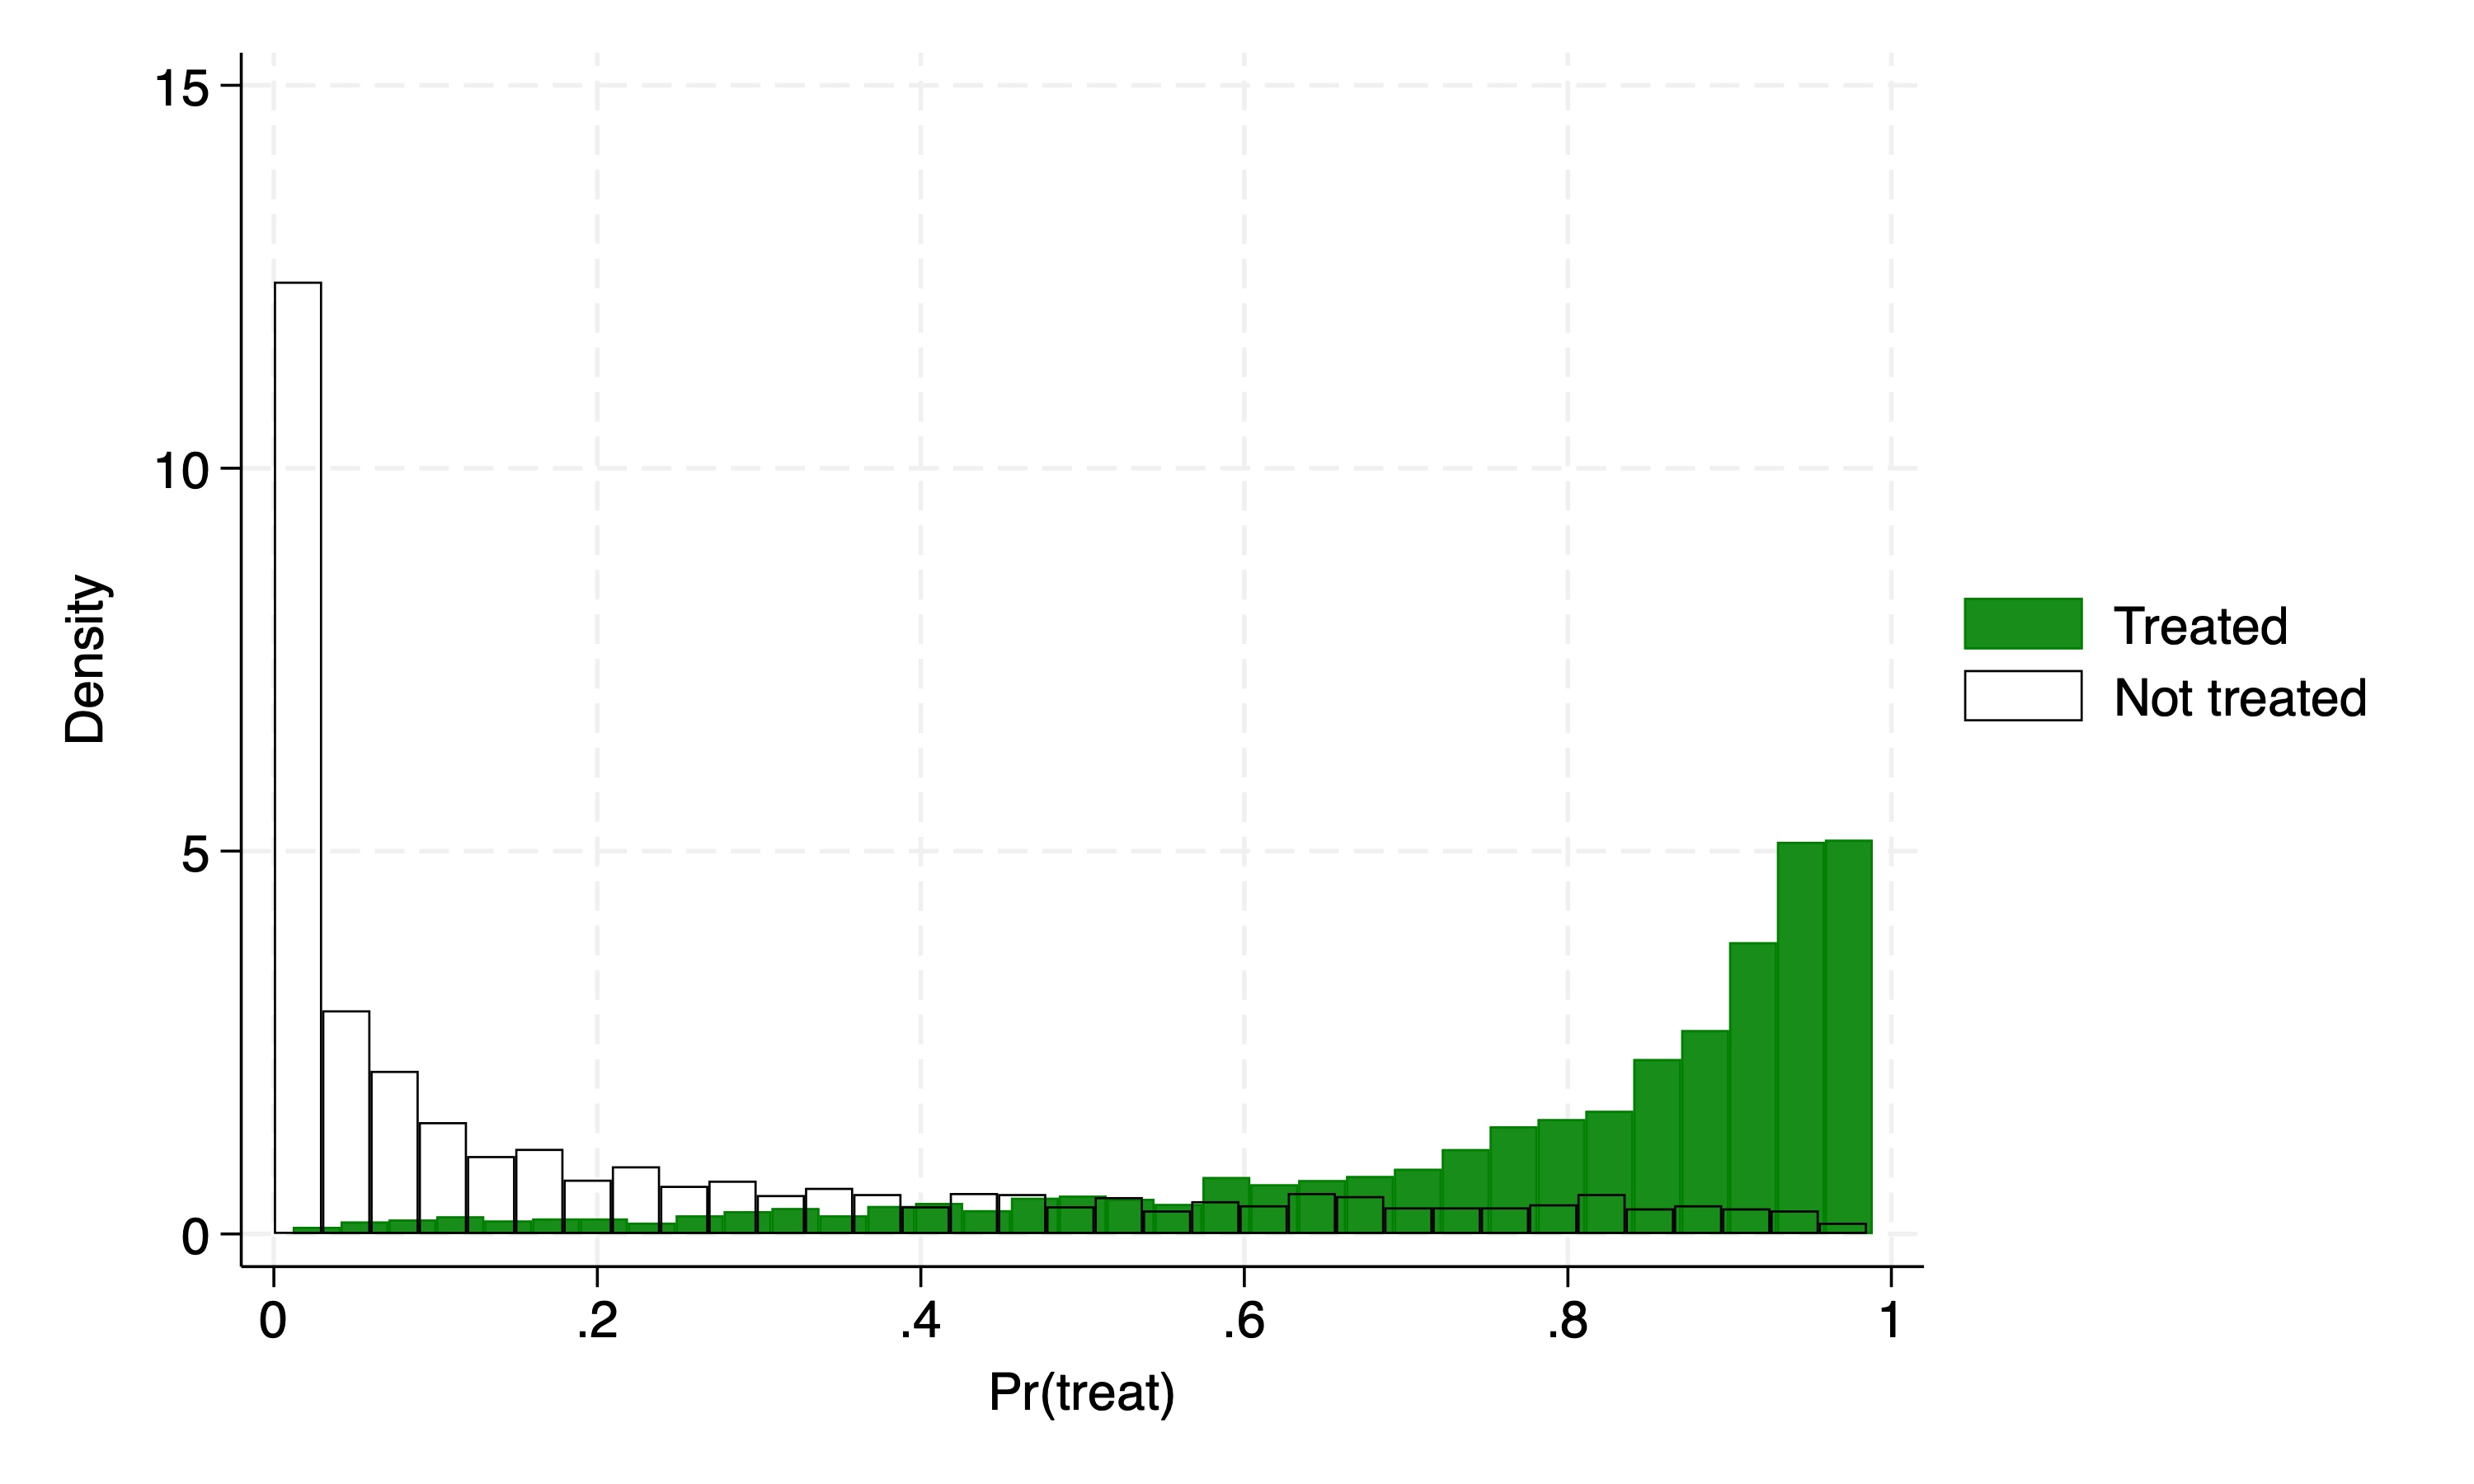
\includegraphics[scale=0.12]{./lecture_includes/pscore_overlap}
\end{figure}

\end{frame}

\begin{frame}{Estimating ATE with IPW}

\begin{itemize}
\item \emph{Any} of the parameters including the ATE are possible with propensity scores

\item Assumptions are strongest for ATE:  full unconfoundedness and full support versus weak versions of both 

\item You should only focus on the ATE if you care about the entire population's treatment effects, but remember that requires more assumptions than if you just focused on the ATT

\end{itemize}

\end{frame}

	


\begin{frame}{Estimating ATE with IPW}

	
		\begin{block}{Estimating ATE with IPW}
	Given $Y^1,Y^0 \independent{D}|X$ and common support, then
		\begin{eqnarray*}
		\delta_{ATE}&=&E[Y^1-Y^0] \\
		&=&E \left[ Y \cdot  \frac{D - \rho(X)}{\rho(X) \cdot (1-\rho(X))} \right]
		\end{eqnarray*}
	\end{block}

Notice that since treated units are missing counterfactuals, but so are controls, all of the data is weighted for the ATE (not just the controls for ATT)

\end{frame}


\begin{frame}{Inverse Probability Weighting}

	\begin{proof}
	\begin{eqnarray*}
	E \left[ Y \cdot \frac{D-\rho(X)}{\rho(X)(1-\rho(X))} \Big\vert X \right] &=& E \left[ \frac{Y}{\rho(X)} \Big\vert X,D=1 \right] \rho(X) \\
	&& + E\left[ \frac{-Y}{1-\rho(X)} \Big\vert X,D=0 \right](1-\rho(X)) \\
	&=& E[Y|X,D=1] - E[Y|X,D=0]
	\end{eqnarray*}and the results follow from integrating over $P(X)$ and $P(X|D=1)$.
	\end{proof}

\end{frame}

\begin{frame}{Other comments about propensity scores}

\begin{itemize}

\item Only other comments to make is that you can get outlier weights
\item If the propensity score is very high for a control group in the ATT, the weight can explode
\item Certain normalizations of the way the IPW is constructed to try and minimize those influences
\item Stata's \texttt{teffects} or R's \texttt{ipw} both let you estimate parameters using IPW and get standard errors
\item But you can do it manually using OLS and use  the propensity scores as analytical weights

\end{itemize}

\end{frame}

\begin{frame}{Simulation}

Lets look at the \texttt{matching.do} again

\end{frame}


\begin{frame}{Double robust estimators}

\begin{itemize}
\item You can have the right covariates but the wrong model and unbiasedness requires the correct model
\item What if you had a way to control for the covariates using propensity scores and something else like regression?
\item Buys you some insurance against model misspecification if such a thing existed
\end{itemize}

\end{frame}

\begin{frame}{Double robust estimators}

\begin{itemize}
\item Question: Is it possible to combine the virtues of regression and propensity score?
\item Answer: Double robust estimators
\item DR address the model misspecification problem by combining propensity scores with other methods 
\item Basic idea in all of them was to control for covariates twice \emph{at the same time} without paying for it (two for one)
\end{itemize}

\end{frame}

\begin{frame}{Double robust estimators}

\begin{itemize}
\item We say that estimators combining regression with IPW are double robust so long as
	\item The regression for the outcome is properly specified, or
	\item The propensity score is properly specified
\item We give ourselves two chances to get it right (either/or not both/and) but if neither is properly specified, then you didn't really gain much
\item Three strikes in baseball
\end{itemize}

\end{frame}

\begin{frame}{Doubly Robust Estimator}
    Easy to verify: with true \( m_1(X) \) (an outcome regression or OR model) and \( \rho(X) \)
\footnotesize

    \[
    ATE = \mathbb{E} \left[ \frac{DY}{\rho(X)} - \frac{D - \rho(X)}{\rho(X)}m_1(X) \right]
    - \mathbb{E} \left[ \frac{(1 - D)Y}{1 - \rho(X)} + \frac{D - \rho(X)}{1 - \rho(X)}m_0(X) \right]
    \]

    \[
    = \mathbb{E} \left[ m_1(X_i) + \frac{D_i\{Y_i - m_1(X_i)\}}{\rho(X_i)} \right]
    - \mathbb{E} \left[ m_0(X_i) + \frac{(1 - D_i)\{Y_i - m_0(X_i)\}}{1 - \rho(X_i)} \right]
    \]

    \[
    = \mu_1 - \mu_0 = \mathbb{E}[Y(1)] - \mathbb{E}[Y(0)]
    \]
\end{frame}

\begin{frame}{Doubly Robust Estimator}
    In the previous formula, replace the true PS \( \rho(X) \) and outcome
    \( m_1(X) \) by the estimated ones from postulated models \( \hat{\rho}(X) \) and
    \( \hat{m}_1(X) \), we obtain two augmented estimators:

    \[
    \widehat{\tau}_{dr} = \hat{\mu}_{1,dr} - \hat{\mu}_{0,dr}
    \]

\footnotesize
    \[
    = \frac{1}{N} \sum_{i=1}^{N} \left[ \frac{D_iY_i - D_i - \hat{\rho}(X_i)}{\hat{\rho}(X_i)} \hat{m}_1(X_i) \right]
    - \frac{1}{N} \sum_{i=1}^{N} \left[ \frac{(1 - D_i)Y_i - D_i - \hat{\rho}(X_i)}{1 - \hat{\rho}(X_i)} \hat{m}_0(X_i) \right]
    \]

\end{frame}

\begin{frame}{Double Robust Estimator}

\begin{itemize}

\item     The two estimators are mathematically the same, but they have different statistical implications:
    	\begin{itemize}
	\item  the first estimator augments an IPW estimator by outcome regression (OR); 
	\item the second augments an OR estimator by IPW.
	\end{itemize}
\item The first estimator is usually referred to as the ``doubly-robust (DR) estimator'' and we saw it in Sant'Anna and Zhou (2020) actually for diff-in-diff

\end{itemize}
\end{frame}


\begin{frame}{Doubly Robust Estimator}
    Now focus on the DR estimator

    Notice that \( \hat{\mu}_{1,dr} \) and \( \hat{\mu}_{0,dr} \) have the same structure

    \[
    \hat{\mu}_{1,dr} = N^{-1} \sum_{i=1}^{N} \left[ \frac{D_iY_i}{\hat{\rho}_i} - \frac{(D_i - \hat{\rho}_i)\hat{m}_1}{\hat{\rho}_i} \right]
    \]

    \[
    \hat{\mu}_{0,dr} = N^{-1} \sum_{i=1}^{N} \left[ \frac{(1 - D_i)Y_i}{1 - \hat{\rho}_i} + \frac{(D_i - \hat{\rho}_i)\hat{m}_0}{1 - \hat{\rho}_i} \right]
    \]

    We will study the properties of \( \hat{\mu}_{1,dr} \) as an estimator for \( \mu_1 = \mathbb{E}\{Y(1)\} \); \( \hat{\mu}_{0,dr} \) is symmetric
\end{frame}




\begin{frame}{Doubly Robust Estimator}
    What does \( \hat{\mu}_{1,dr} \) estimate? Simple algebra shows that \( \mu_{1, dr} \) converges to

    \[
    \mathbb{E}\left[ \frac{DY}{\rho(X)} - \frac{D - \rho(X)}{\rho(X)}m(X) \right]
    \]

    \[
    = \mathbb{E}\{Y(1)\} + \mathbb{E}\left[ \frac{D - \rho(X)}{\rho(X)}\{Y(1) - m(X)\} \right]
    \]


\begin{itemize}
\item     Thus, in order for \( \hat{\mu}_{1,dr} \) to estimate \( \mathbb{E}\{Y(1)\} \), the second term in (4) must be 0

\item     Regression estimator augmented by weighted residuals

\item     When does the second term $=$ 0?

\end{itemize}
\end{frame}

\begin{frame}{Doubly Robust Estimator}
    When does \( R = \mathbb{E} \left[ \frac{D - \rho(X)}{\rho(X)} \{Y(1) - m_1(X)\} \right] = 0? \)

    \begin{itemize}
        \item \textbf{Scenario 1:} Postulated propensity score model \( \rho(X; \beta) \) is
        incorrect, but postulated regression model \( m_1(X; \alpha) \) is correct

        \[
        R = \mathbb{E} \left[ \mathbb{E} \left[ \frac{D - \rho(X)}{\rho(X)} \{Y(1) - m_1(X)\} \middle| X \right] \right]
        \]

        \[
        = \mathbb{E} \left[ \frac{\rho_{true}(X) - \rho(X)}{\rho(X)} \mathbb{E} \{Y(1) - m_1(X) \middle| X\} \right]
        \]

\item Easy to see that \( \mathbb{E} \{Y(1) - m_1(X) | X\} = \mathbb{E} \{Y(1) | X\} - m_1(X) = m_{1,true}(X) - m_1(X) = 0 \)

    \end{itemize}
\end{frame}


\begin{frame}{Doubly Robust Estimator}
    When does \( \mathbb{E} \left[ \frac{D - \rho(X)}{\rho(X)} \{Y(1) - m_1(X)\} \right] = 0? \)

    \begin{itemize}
        \item \textbf{Scenario 2:} Postulated propensity score model \( \rho(X; \beta) \) is correct,
        but postulated regression model \( m_1(X; \alpha) \) is incorrect

        \[
        R = \mathbb{E} \left[ \mathbb{E} \left[ \frac{D - \rho(X)}{\rho(X)} \{Y(1) - m_1(X)\} \middle| X \right] \right]
        \]

        \[
        = \mathbb{E} \left[ \frac{\rho_{true}(X) - \rho(X)}{\rho(X)} \mathbb{E} \{Y(1) - m_1(X) \middle| X\} \right]
        \]

        \item Equals to zero because \( \rho_{true}(X) - \rho(X) = 0 \)
    \end{itemize}
\end{frame}




\begin{frame}{Doubly Robust Estimator}
    \begin{itemize}
        \item In both cases, the second term goes to 0 in large samples, and
        thus \( \hat{\mu}_{1,dr} \) is consistent (asymptotically unbiased) for \( E(Y(1)) \).
        \item Similarly, \( \hat{\mu}_{0,dr} \) is consistent for \( E(Y(0)) \), and hence \( \hat{\tau}_{dr} \)
        is consistent for the ATE.
        \item Obviously, if both models are correct, \( \hat{\tau}_{dr} \) is consistent for
        estimating the ATE.
    \end{itemize}
\end{frame}




\begin{frame}{Doubly Robust Estimator}
    \textbf{Double Robustness:} \( \hat{\tau}_{dr} \) is a consistent estimator of the ATE if either
    the propensity score model or the potential outcome model is, but not
    necessarily both are, correctly specified

    \begin{itemize}
        \item DR is a large sample property
        \item Offers protection against model mis-specification: gives you two
        chances to get it right (and wrong)!
        \item If \( \rho(X) \) and \( m_1(X) \) are modeled correctly, \( \hat{\tau}_{dr} \) will have smaller
        variance than the IPW estimator (in large samples)
        \item If the outcome model \( m_1(X) \) is correct, \( \hat{\tau}_{dr} \) has larger variance (in
        large samples) than the direct regression estimator
        \item ... but gives protection in the event it is not
    \end{itemize}
\end{frame}








\begin{frame}{Propensity score matching}
	
	\begin{itemize}
	\item Matching, or ``imputation'', is another way that utilizes the $\widehat{\rho_i}(X_i)$
	\item Matching estimation based on the propensity score has the same first step as IPW, but not the second and third steps
	\item Common support starts to be more complex with imputation methods because you will need to decide how far away from a unit's own propensity score is a tolerable distance to be considered a ``neighbor''
	\end{itemize}

\end{frame}




\begin{frame}{Standard matching strategy}
	
	\begin{itemize}
	\item Pair each treatment unit $i$ with one or more \emph{comparable} control group unit $j$, where comparability is in terms of proximity, or distance, to the estimated propensity score
	\item Impute the unit's missing counterfactual outcome $Y_{i(j)}$ based on the unit or units chosen in the previous step
	\item If more than one are ``nearest neighbors'', then use the neighbors' weighted outcomes  $$Y_{i(j)} = \sum_{j \in C(i)} w_{ij}Y_j$$ where $C(i)$ is the set of neighbors with $W=0$ of the treatment unit $i$and $w_{ij}$ is the weight of control group units $j$ with $\sum_{j \in C(i)} w_{ij} = 1$
	\end{itemize}
\end{frame}


\begin{frame}{Imputing the counterfactuals}
	
	Let the ATT be our parameter of interest: $$E[Y^1_i | D_i=1] - E[Y^0_i | D_i=1]$$We estimate it as follows  $$\widehat{ATT} = \frac{1}{N_T}  \sum_{i:D_i=1} \bigg [Y_i - Y_{i(j)} \bigg ]$$where $N_T$ is the number of matched treatment units in the sample. Note the difference between \emph{imputation} and IPW -- the only weight here is $\frac{1}{N_T}$

\end{frame}

\begin{frame}{Matching methods}
	
	\begin{itemize}
	\item The probability of observing two units with \emph{exactly} the same propensity score is in principle zero if $Pr(X=x)$ is continuous
	\item Several matching methods have been proposed in the literature, but the most widely used are:
		\begin{itemize}
		\item Stratification matching
		\item Nearest-neighbor matching (with or without caliper)
		\item Radius matching
		\item Kernel matching
		\end{itemize}
	\item Typically, one treatment unit $i$ is matched to several control units $j$, but sometimes one-to-one matching is used
	\end{itemize}
	
\end{frame}


\begin{frame}{Stratification}
	
	\begin{itemize}
	\item Stratification based on the propensity score is a multi step process that bears resemblance to the stratification/subclassification method proposed by Cochran (1968)
	\item  Method uses brute force to achieve the balancing property discussed earlier, which is then used with weighted differences in means within propensity score ``strata''
	\item Dehejia and Wahba (2002) used stratification matching in their seminal paper 
	\end{itemize}
	
\end{frame}


\begin{frame}{Stratification: Achieving Balance}
	
First create ``propensity score strata'' inside which you have balanced covariates
	\begin{enumerate}
		\item Sort the data by propensity score and divide into groups of observations with similar propensity scores (e.g., percentiles)
		\item Within each strata, test (e.g., t-test) whether the means of the $k$ covariates are equal between treatment and control
		\item If so, then stop.  If not, it means the covariates aren't balanced \emph{within that propensity score strata} so then divide that strata in half and repeat step 2
		\item If a particular covariate is unbalanced for multiple groups, modify the initial logit or probit equation by including higher order terms and/or interactions with that covariate and repeat
		\end{enumerate}

\end{frame}

\begin{frame}{Propensity score matching}
	
	\begin{itemize}
	\item Next we review explicit imputation based on the propensity score or what is sometimes called propensity score matching
	\item King and Nielsen (2019) is a critique of using propensity scores \emph{for matching} (i.e., imputation)
	\item But not a critique of the propensity score itself or to stratification, regression adjustment, or IPW
	\item Issues raised have to do with forced balance through trimming and a myriad of other common choices made by the researcher
	\end{itemize}
	
\end{frame}

\begin{frame}{Ad hoc user choices introduce bias}

\begin{quote}
	
``[The] more balanced the data, or the more balance it becomes by [trimming] some of the observations through matching, the more likely propensity score matching will degrade inferences.'' -- King and Nielsen (2019)

\end{quote}
	
\end{frame}



\begin{frame}{Nearest Neighbor}
	
	Pretty similar to covariate matching.  Formula is $$\widehat{ATT} = \frac{1}{N_T} \sum_{i:D_i=1} \bigg [ Y_i - \sum_{j \in C(i)_M} w_{ij}Y_j \bigg ]$$ 
		\begin{itemize}
		\item $N_T$ is the number of treated units $i$ and  $N_C$ is number of control units $j$
		\item $w_{ij}$ is equal to $\frac{1}{N_C}$ if $j$ is a control unit and zero otherwise
		\item And unit $j$ is chosen as a control for $i$ if it's propensity score is nearest to that of $i$
		\end{itemize}
\end{frame}

\begin{frame}{NN Matching: Bias vs. Variance}
	
How far away on the propensity score will you use is what makes some of the different types of matching proposed differ
		\begin{itemize}
		\item Matching just one nearest neighbor minimizes bias at the cost of larger variance
		\item Matching using additional nearest neighbors increases the bias but decreases the variance
		\end{itemize}
	
\end{frame}

\begin{frame}{NN Matching: Bias vs. Variance}
	
	 Matching with or without replacement
		\begin{itemize}
		\item with replacement keeps bias low at the cost of larger variance
		\item without replacement keeps variance low but at the cost of potential bias
		\end{itemize}
	
\end{frame}



\begin{frame}{Distance between treatment and control units}

\begin{itemize}
\item What was historically done was limiting ``distance''  through various \emph{ad hoc} choices
\item Imagine these choices as creating like a cowboy rope lasso that matches to everything inside that circle
\item There were two common ways for creating the circle -- caliper matching and radius matching. 
\end{itemize}

\end{frame}

\begin{frame}{Caliper matching}
	
	\begin{itemize}
	\item Caliper matching is a variation on NN matching that tries to build brakes into the algorithm as to avoid ``bad neighbors'' by imposing a tolerable maximum distance (e.g., 0.2 units in the propensity score away from a treatment unit $i$'s propensity score)
	\item Note -- this is a one-to-one imputation, and if there doesn't exist anybody in the control group unit $j$ within that ``caliper'', then treatment unit $i$ is discarded which as with all trimming changes the parameter we are estimating
	\item It's difficult to know what this caliper should be \emph{ex ante}, hence why I said it is somewhat \emph{ad hoc}
	\end{itemize}

\end{frame}


\begin{frame}{Radius matching}
	
	
		\begin{itemize}
		\item Each treatment unit $i$ is matched with the control group units whose propensity score are in a ``predefined neighborhood'' of the propensity score of the treatment unit.
		\item \textbf{All} the control units with $\widehat{\rho_j}(X_{j})$ falling within a radius $r$ from $\widehat{\rho}_i(X_i)$ are matched to the treatment unit $i$ -- this is what distinguishes it from calipers, and makes it more similar to covariate matching (Abadie and Imbens 2006, 2008)
		\item The smaller the radius, the better the quality of the matches, but the higher the possibility some treatment units are not matched because the neighborhood does not contain control group units $j$
		\end{itemize}
		
\end{frame}

\begin{frame}{Software}

\begin{itemize}
\item You can use -\texttt{teffects, psmatch}- to get at these two nearest neighbor approaches by setting the number of matches
\item You can use -\texttt{pscore2}- for stratification
\item You can use the \texttt{MatchIt} package in R
\end{itemize}

\end{frame}





		  

\begin{frame}{Failure of econometric estimators (LaLonde 1986)}
	
	\begin{itemize}
	\item Evaluation of the Job Trainings Program (NSW) has a rich history in causal inference
	\item Bob LaLonde (passed away November 2015) was a Card and Ashenfelter student at Princeton whose job market paper evaluated, not NSW itself, but econometric methods one would use in something like NSW
	\item Dehejia and Wahba (1999; 2002) used LaLonde's data with propensity score matching and found they could recover known effects
	\item Critiques by Petra Todd, Jeff Smith and others followed which I'll summarize
	\end{itemize}
\end{frame}

\begin{frame}{Summarizing LaLonde (1986)}

		\begin{itemize}
		\item Very clever study that combined experimental and non-experimental data to ascertain whether popular econometric methods could recover unbiased effects when those effects were already known 
		\item Damning conclusion -- 1986 AER (it was LaLonde's JMP) found econometric methods failed to get the number right, and worse, failed to get the sign right
		\item Was a critical paper in the emerging ``credibility crisis'' within labor and helped fuel the type of work we now broadly consider to be design based causal inference
		\end{itemize}

\end{frame}

\begin{frame}[plain]
	\begin{center}
	LaLonde, Robert J. (1986). \myurlshort{http://business.baylor.edu/scott_cunningham/teaching/lalonde-1986.pdf}{``Evaluating the Econometric Evaluations of Training Programs with Experimental Data''}. \emph{American Economic Review}. 
	\end{center}
	
\underline{LaLonde's study} was \textbf{not} an evaluation of the NSW program, as that had been done, but rather an evaluation of econometric models done by:
		\begin{itemize}
		\item replacing the experimental NSW control group with non-experimental control group drawn from two nationally representative survey datasets: Current Population Survey (CPS) and Panel Study of Income Dynamics (PSID)
		\item estimating the average effect using non-experimental workers as controls for the NSW trainees 
		\item comparing his non-experimental estimates to the experimental estimates of \$900
		\end{itemize}
\end{frame}

\begin{frame}{LaLonde (1986)}

\begin{itemize}

	\item \underline{LaLonde's conclusion}: available econometric approaches were biased and inconsistent
		\begin{itemize}
		\item His estimates were way off and usually the wrong sign
		\item Conclusion was influential in policy circles and led to greater push for more experimental evaluations
		\end{itemize}

\end{itemize}

\end{frame}


\begin{frame}{Description of NSW Job Trainings Program}
	
The National Supported Work Demonstration (NSW), operated by Manpower Demonstration Research Corp in the mid-1970s:
	\begin{itemize}
	\item was a temporary employment program designed to help disadvantaged workers lacking basic job skills move into the labor market by giving them work experience and counseling in a sheltered environment
	\item was also unique in that it \textbf{randomly assigned} qualified applicants to training positions:
		\begin{itemize}
		\item \textbf{Treatment group}: received all the benefits of NSW program
		\item \textbf{Control group}: left to fend for themselves
		\end{itemize}
	\item admitted AFDC females, ex-drug addicts, ex-criminal offenders, and high school dropouts of both sexes
	\end{itemize}
\end{frame}

\begin{frame}{NSW Program}
	
	\begin{itemize}
	\item Treatment group members were:
		\begin{itemize}
		\item guaranteed a job for 9-18 months depending on the target group and site
		\item divided into crews of 3-5 participants who worked together and met frequently with an NSW counselor to discuss grievances and performance
		\item paid for their work
		\end{itemize}
	\item Control group members were randomized so the same
	\item Note: the randomization balanced observables and unobservables across the two arms, thus enabling the estimation of an ATE for the people who self-selected into the program
	\end{itemize}
\end{frame}

\begin{frame}{NSW Program}

\begin{itemize}
	\item Other details about the NSW program:
		\begin{itemize}
		\item \underline{Wages}:  NSW offered the trainees lower wage rates than they would've received on a regular job, but allowed their earnings to increase for satisfactory performance and attendance
		\item \underline{Post-treatment}: after their term expired, they were forced to find regular employment
		\item \underline{Job types}:  varied within sites -- gas station attendant, working at a printer shop -- and males and females were frequently performing different kinds of work
		\end{itemize}
\end{itemize}

\end{frame}
	
\begin{frame}{NSW Data}
	
	\begin{itemize}
	\item \underline{NSW data collection}:
		\begin{itemize}
		\item MDRC collected earnings and demographic information from both treatment and control at baseline and every 9 months thereafter
		\item Conducted up to 4 post-baseline interviews
		\item Different sample sizes from study to study can be confusing, but has simple explanations
		\end{itemize}
	\end{itemize}
\end{frame}
	

\begin{frame}{NSW Data}

\begin{itemize}
	\item \underline{Estimation}:
		\begin{itemize}
		\item NSW was a randomized job trainings program; therefore estimating the average treatment effect is straightforward:
			\begin{eqnarray*}
			SDO = \frac{1}{N_t}\sum_{D_i=1}Y_i - \frac{1}{N_c}\sum_{D_i=0}Y_i \approx E[Y^1-Y^0] 
			\end{eqnarray*}in large samples assuming treatment selection is independent of potential outcomes (randomization) -- i.e., $(Y^0,Y^1)\independent{D}$. 
		\end{itemize}
	\item \underline{NSW worked}: Treatment group participants' real earnings post-treatment (1978) was positive and economically meaningful -- $\approx$ \$900 (LaLonde 1986) to \$1,800 (Dehejia and Wahba 2002) depending on the sample used
\end{itemize}

\end{frame}
	
\imageframe{./lecture_includes/lalonde_table5a.png}


\begin{frame}{Switching out the control group}

\begin{itemize}
\item Think of \$800 to \$900 as the ``ground truth'' since row 1 was using the RCT 
\item LaLonde ``drops'' the experimental controls (which satisfied independence) and ``replaces'' it with six different draws from two nationally representative surveys (PSID and CPS)
\item Now the dataset contains a negatively selected treatment group compared to a nationally representative control group
\item Will selection on observable methods ``work''?
\end{itemize}

\end{frame}


\imageframe{./lecture_includes/lalonde_table5b.png}

\begin{frame}[plain,shrink=10]{Imbalanced covariates for experimental and non-experimental samples}

    \begin{center}
		\begin{table}
		\begin{tabular}{lcccccc}
		\hline \hline
		\multicolumn{3}{c}{}&
		\multicolumn{1}{c}{CPS}&
		\multicolumn{1}{c}{NSW}\\
		
		\multicolumn{1}{c}{}&
		\multicolumn{2}{c}{All} &
		\multicolumn{1}{c}{Controls} &
		\multicolumn{1}{c}{Trainees} \\

		\multicolumn{3}{c}{}&
		\multicolumn{1}{c}{$N_c=15,992$}&
		\multicolumn{1}{c}{$N_t=297$}&
		\multicolumn{1}{c}{}&
		\multicolumn{1}{c}{}\\

		\multicolumn{1}{l}{covariate}&
		\multicolumn{1}{c}{mean}&
		\multicolumn{1}{c}{(s.d.)}&
		\multicolumn{1}{c}{mean}&
		\multicolumn{1}{c}{mean}&
		\multicolumn{1}{c}{t-stat}&
		\multicolumn{1}{c}{diff}\\
		\hline
Black    & 0.09 & 0.28 & 0.07 & 0.80 & 47.04 & -0.73\\
Hispanic & 0.07 & 0.26 & 0.07 & 0.94 & 1.47 & -0.02\\
Age & 33.07 & 11.04 & 33.2 & 24.63 & 13.37  & 8.6\\
Married & 0.70 & 0.46 & 0.71 & 0.17 & 20.54 & 0.54\\
No degree & 0.30 & 0.46 & 0.30 & 0.73 & 16.27 & -0.43\\
Education & 12.0 & 2.86 & 12.03 & 10.38 & 9.85 & 1.65 \\
1975 Earnings   & 13.51 & 9.31 & 13.65 & 3.1 & 19.63 & 10.6\\
1975 Unemp  & 0.11 & 0.32 & 0.11 & 0.37 & 14.29 & -0.26\\
		\hline 
		\end{tabular}
		\end{table}
    \end{center}

\end{frame}


\begin{frame}{Dehija and Wahba (1999)}
	
	\begin{itemize}
	\item Dehejia and Wahba (DW) update LaLonde's original study using propensity score matching
		\begin{enumerate}
		\item Dehejia, Rajeev H. and Sadek Wahba (1999). 	``Causal Effects in Nonexperimental Studies: Reevaluating the Evaluation of Training Programs''. \underline{Journal of the American Statistical} \underline{Association}, vol. 94(448): 1053-1062 (\myurlshort{http://business.baylor.edu/scott_cunningham/teaching/dehejia-and-wahba-1999.pdf}{pdf})
		\end{enumerate}
	\item Can propensity score matching improve over the estimators that LaLonde examined?
	\end{itemize}
\end{frame}

\begin{frame}[plain]
	
\begin{figure}
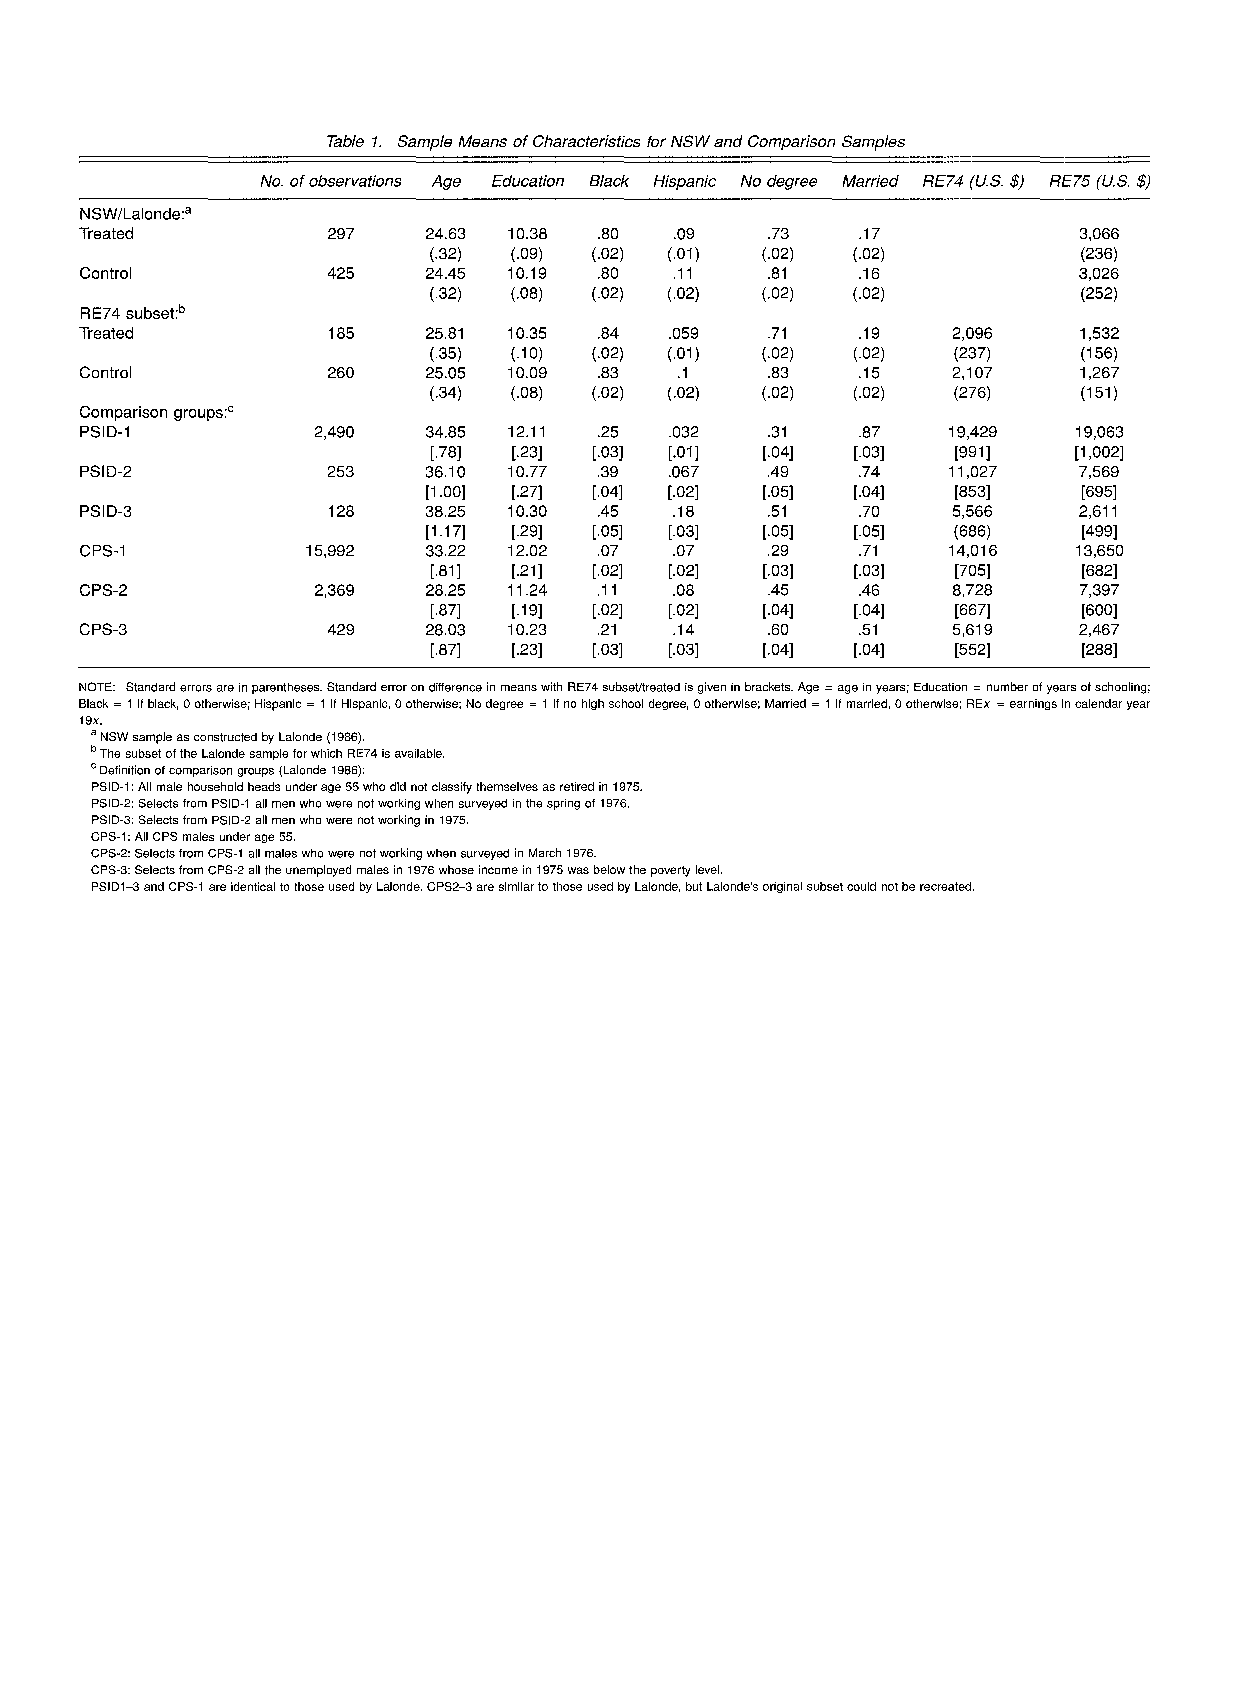
\includegraphics[scale=0.5]{./lecture_includes/dw_1.pdf}
\end{figure}

\end{frame}

\imageframe{./lecture_includes/dw_2.pdf}

\begin{frame}{Covariate imbalance}
	

	\begin{itemize}
	\item Conditional on the propensity score, the covariates are independent of the treatment, suggesting that the distribution of covariate values should be the same for both treatment and control groups
	\item This can be checked as we have data on all three once we've estimated the propensity score
	\item DW note that the two samples have \emph{severe} imbalance on \emph{observables} -- a huge number of non-experimental controls have propensity scores almost exactly equal to 0
	\item Their analysis will ``trim'' (which will ultimately have implications for interpretation)
	\end{itemize}

\end{frame}



\imageframe{./lecture_includes/dw_3.pdf}
\imageframe{./lecture_includes/dw_4.pdf}
\imageframe{./lecture_includes/dw_5.pdf}
\imageframe{./lecture_includes/dw_6.pdf}



\clearpage
\newpage

\begin{frame}{Replies by econometricians to DW}

\begin{itemize}
\item Heckman, Smith and Todd concluded from their own work that in order for matching estimators to have low bias, you need the following:
	\begin{enumerate}
	\item A rich set of variables related to program participation and predictive of $Y^0$ labor market outcomes, 
	\item Nonexperimental comparison group be drawn from the same local labor markets as the participants and 
	\item Dependent variable (e.g., earnings) be measured in the same way for participants and nonparticipants
	\end{enumerate}
\item All three of these conditions fail to hold in DW (1999, 2002) according to Smith and Todd (2005)
\item DW also note the importance of conditioning on pre-treatment lagged outcomes (e.g., real earnings in $t-1$, $t-2$, etc.) as well as \emph{trimming}
\end{itemize}

\end{frame}


\begin{frame}{Smith and Todd, diff-in-diff, doubly robust}

\begin{itemize}
\item Difference-in-differences with propensity scores tended to work well in Smith and Todd (2005) though the effect sizes are much larger
\item In my Causal Inference II workshop, we use Sant'anna And Zhao's double robust DiD and get nearly the exact same parameter estimate as the experimental finding

\end{itemize}

\end{frame}

\begin{frame}{Coding together}

\begin{itemize}

\item Let's spend some time together trying to replicate the Lalonde study ourselves
\item I use replicate lightly -- our goal is syntax only
\item It's in the Lalonde lab on githbub for this workshop

\end{itemize}

\end{frame}


\subsection{Regressions}



\begin{frame}{Interpreting OLS coefficients}

\begin{itemize}
\item Most common causal model is OLS with covariate controls 


		\begin{align*}
		Y_i = \beta_0 + \beta_1 X_i + u_i&\\
		\end{align*}

\item OLS is the best linear predictor (Angrist and Pischke 2009)
\item But the best linear predictor of the \emph{realized} outcome is not the same as being the best linear predictor of the \emph{missing potential outcome}

\end{itemize}

\end{frame}



\begin{frame}{OLS Simulated Code}

\begin{figure}[!t]\centering
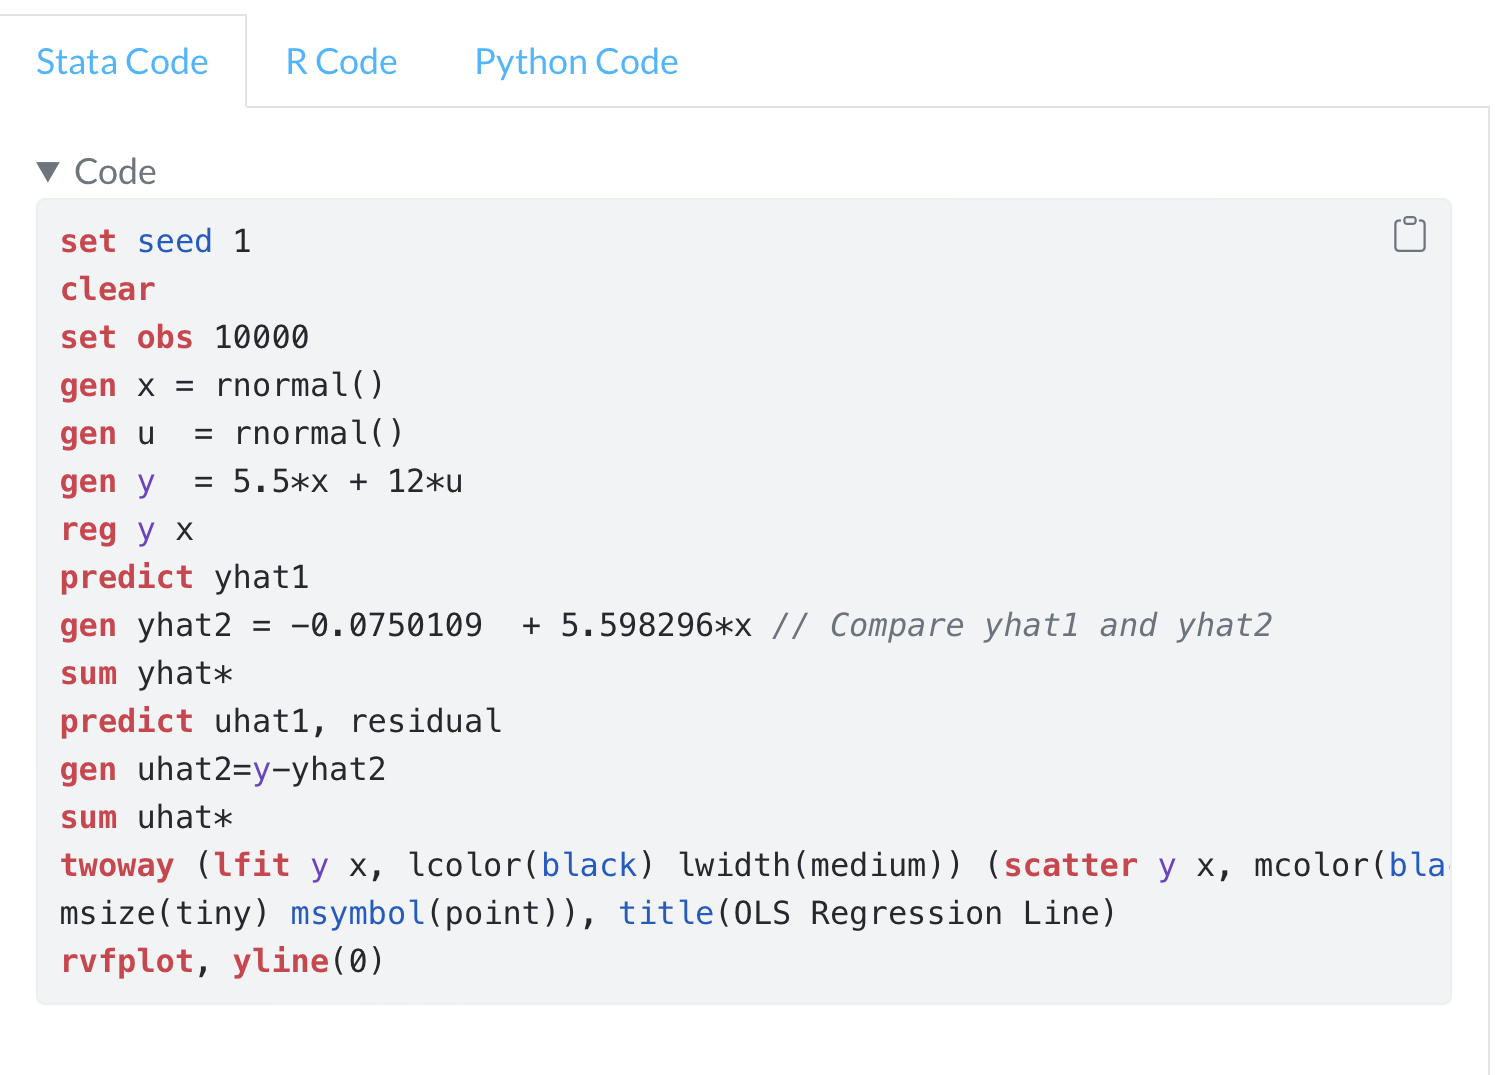
\includegraphics[scale=0.40]{./lecture_includes/ols_code}
\end{figure}

\end{frame}

\begin{frame}{OLS Extrapolates Using Functional Form (e.g., Lines)}

\begin{figure}[!t]\centering
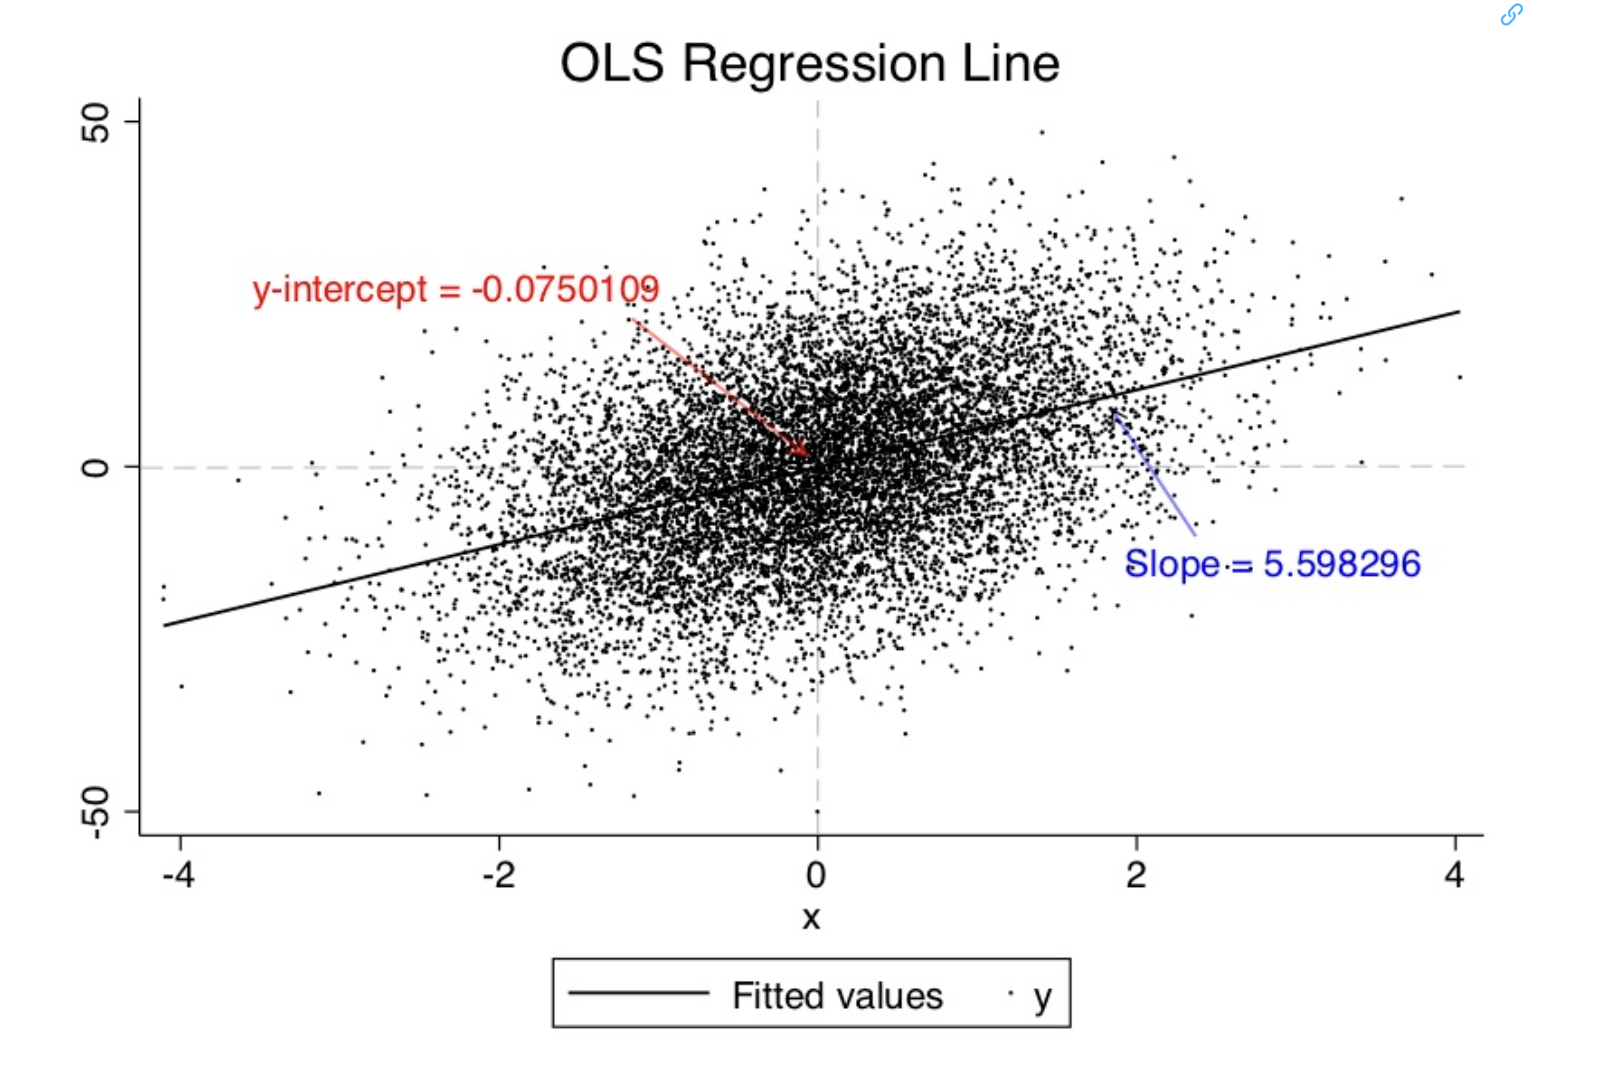
\includegraphics[scale=0.4]{./lecture_includes/ols_line}
\end{figure}

\end{frame}

\begin{frame}{Bivariate vs multivariate regressions}

\begin{itemize}

\item Interpreting the OLS coefficient in bivariate regression is written out as a scaled covariance:

 $$\widehat{\beta_1}=\frac{Cov(Y_i,X_i)}{Var(X_i)}$$
 
 \item But when we are looking at a multivariate regression, what is it?
 
 \end{itemize}
 
 \end{frame}
 
 \begin{frame}{Applying FWL theorem}

\begin{itemize}
\item Frisch-Waugh-Lovell also helps us interpret $\widehat{\beta}_1$ when there are covariates
 \item Use the FWL theorem to turn the multivariate regression coefficient into the simple bivariate one
\item Angrist and Pischke (2009) call FWL the ``regression anatomy theorem'' and Filoso (2013) has an excellent and original proof
\end{itemize}

\end{frame}



\begin{frame}{Applying FWL theorem}

	\begin{itemize}
	\item Can we estimate the causal effect of family size on labor supply by regressing labor supply (\texttt{Y}) on family size (\texttt{X})?
		\begin{eqnarray*}
		Y_i = \beta_0 + \beta_1 X_i + u_i&\\
		\end{eqnarray*}
	\item If family size is random, then we can interpret $\widehat{\beta_1}$ as the ATE
	\item But how do we interpret $\widehat{\beta_1}$ if \texttt{family size} is only conditionally random?  
	\end{itemize}
\end{frame}


\begin{frame}{Applying FWL theorem}
	
	\begin{itemize}
	\item Assume the longer model is:
		\begin{eqnarray*}
Y_i &=& \beta_0 + \beta_1 X_i + \gamma_1 \texttt{White}_i + \gamma_2 \texttt{Married}_i \\
		& & + \gamma_3 \texttt{Age}_i + \gamma_4 \texttt{Employed}_i + u_i
		\end{eqnarray*}
	\item Assume unconfoundedness and constant treatment effects so that family size is independent conditional on all controls
	\item FWL shows that in a multivariate regression, any one coefficient fitted can be reconceived as a simple scaled covariance of the outcome and residualized treatment variable
	\end{itemize}
	
\end{frame}




		

\begin{frame}{FWL Theorem}

	\begin{block}{FWL Theorem }
	Assume your main multiple regression model of interest:$$y_i=\beta_0 + \beta_1x_{1i} + \dots + \beta_kx_{ki} + \dots + \beta_Kx_{Ki} + e_i$$ and an auxiliary regression in which the variable $x_{1i}$ is regressed on all the remaining independent variables$$x_{1i} = \gamma_0 + \gamma_{k-1}x_{k-1 i}+\gamma_{k+1}x_{k+1 i} + \dots + \gamma_Kx_{Ki}+f_i$$and $\tilde{x}_{1i} = x_{1i} - \widehat{x}_{1i}$ being the residual from the auxiliary regression. The parameter $\beta_1$ can be rewritten as:$$\beta_1=\frac{Cov(y_i,\tilde{x}_{1i})}{Var(\tilde{x}_{1i})}$$

	\end{block}

\end{frame}


\begin{frame}[plain, shrink=20]

\bigskip

	\begin{block}{FWL Proof  (Proof by Filoso 2013)}
	To prove the theorem, note $E[\tilde{x}_{ki}]=E[x_{ki}]-E[\widehat{x}_{ki}]=E[f_i]$, and plug $y_i$ and residual $\tilde{x}_{ki}$ from $x_{ki}$ auxiliary regression into the covariance $cov(y_i, \tilde{x}_{ki})$
	\begin{eqnarray*}
	\beta_k &=& \frac{ cov(y_i, \tilde{x}_{ki})}{var(\tilde{x}_{ki})} \\
			 &=& \frac{ cov(\beta_0 + \beta_1x_{1i} + \dots + \beta_kx_{ki} + \dots + \beta_Kx_{Ki} + e_i, \tilde{x}_{ki})}{var(\tilde{x}_{ki})} \\
			&=& \frac{ cov(\beta_0 + \beta_1x_{1i} + \dots + \beta_kx_{ki} + \dots + \beta_Kx_{Ki} + e_i,f_i)}{var(f_i)}
	\end{eqnarray*}
	\begin{enumerate}
	\item Since by construction $E[f_i]=0$, it follows that the term $\beta_0E[f_i]=0$.
	\item Since $f_i$ is a linear combination of all the independent variables with the exception of $x_{ki}$, it must be that$$\beta_1E[f_ix_{1i}] = \dots = \beta_{k-1}E[f_ix_{k-1 i}] = \beta_{k+1}E[f_ix_{k+1 i}] = \dots = \beta_KE[f_ix_{KI}] = 0$$
	\end{enumerate}
	\end{block}
\end{frame}


\begin{frame}[plain, shrink=20]

	\begin{block}{FWL Proof  (Proof by Filoso 2013)}
		\begin{enumerate}\addtocounter{enumi}{2}
		\item Consider now the term $E[e_if_i]$.  This can be written as:
			\begin{eqnarray*}
			E[e_if_i] &=& E[e_if_i] \\
			&=& E[e_i\tilde{x}_{ki}] \\
			&=& E[e_i(x_{ki} - \widehat{x}_{ki})] \\
			&=& E[e_ix_{ki}] - E[e_i\tilde{x}_{ki}]
			\end{eqnarray*}Since $e_i$ is uncorrelated with any independent variable, it is also uncorrelated with $x_{ki}$: accordingly, we have $E[e_ix_{ki}]=0$. With regard to the second term of the subtraction, substituting the predicted value from the $x_{ki}$ auxiliary regression, we get$$E[e_i\tilde{x}_{ki}] = E[e_i(\widehat{\gamma_0} + \widehat{\gamma_1}x_{1i} + \dots + \widehat{\gamma}_{k-1}x_{k-1}i+\widehat{\gamma}_{k+1}x_{k+1 i} + \dots + \widehat{\gamma}_Kx_{Ki})]$$Once again, since $e_i$ is uncorrelated with any independent variable, the expected value of the terms is equal to zero.  Then, it follows $E[e_if_i]=0$.
		
		\end{enumerate}
	\end{block}

\end{frame}

\begin{frame}[plain, shrink=25]

	\begin{block}{FWL Proof  (Proof by Filoso 2013)}
		\begin{enumerate}\addtocounter{enumi}{3}
		\item The only remaining term is $E[\beta_kx_{ki}f_i]$ which equals $E[\beta_kx_{ki}\tilde{x}_{ki}]$ since $f_i=\tilde{x}_{ki}$. The term $x_{ki}$ can be substituted using a rewriting of the auxiliary regression model, $x_{ki}$, such that$$x_{ki} = E[x_{ki} | X_{-k}] + \tilde{x}_{ki}$$This gives
			\begin{eqnarray*}
			E[\beta_kx_{ki}\tilde{x}_{ki}] &=& E[\beta_kE[\tilde{x}_{ki}(E[x_{ki}|X_{-k}]+\tilde{x}_{ki})]] \\
			&=& \beta_kE[\tilde{x}_{ki}(E[x_{ki}|X_{-k}]+\tilde{x}_{ki})] \\
			&=&\beta_k\{E[\tilde{x}^2_{ki}] + E[(E[x_{ki}|X_{-k}]\tilde{x}_{ki})]\} \\
			&=& \beta_k var(\tilde{x}_{ki})
			\end{eqnarray*}which follows directly from the orthogonoality between $E[x_{ki} | X_{-k}]$ and $\tilde{x}_{ki}$. From previous derivations we finally get$$cov(y_i,\tilde{x}_{ki}) = \beta_kvar(\tilde{x}_{ki})$$which completes the proof. \qedhere
		\end{enumerate}
	\end{block}

\end{frame}

\begin{frame}{FWL}

\begin{itemize}
\item Let's review the FWL ``partialing out'' interpretation of OLS estimated $\widehat{\beta_1}$ in code
\item We will use the fwl.do at /Labs/Matching for this
\end{itemize}

\end{frame}



\begin{frame}{Core OLS assumptions}

\begin{itemize}
\item Return to OLS model with additive covariates  controls: $$Y_i = \alpha + \delta D_i + \beta X_i + \gamma Z_i + \varepsilon_i$$
\item Which average treatment effect parameter does $\widehat{\delta}$ estimate?  What assumptions are imposed by exogeneity?
\item This hopefully is where I'll be able to convince you of how important it is that you identify ahead of time \emph{which} causal effect
\item This is \textbf{not} a criticism of OLS but rather of that specification above
\end{itemize}

\end{frame}

\begin{frame}{OLS Assumptions}

\begin{itemize}

\item Typically we assume that the mean error is zero conditional on all covariates, called exogeneity
\item This is a pregnant assumption as it turns out
\item Imbens and Rubin discussed it in their book on causal inference from 2015
\item I'll pull out their quote and proof but we will then discuss some other materials

\end{itemize}

\end{frame}


\begin{frame}{OLS Assumptions}

	\begin{quote} 
	``In many empirical studies in social sciences, causal effects are estimated through linear regression, where, typically it is implicitly assumed that in the super-population, $$E[Y_i^D | X_i] = \alpha + \delta_{sp} \cdot D + X_i \beta$$ for some values of the three unknown parameters, $\alpha$, $\delta_{sp}$ and $\beta$ where $\delta_{sp} = E_{sp} [ Y_i^1 - Y_i^0]$.''
	\end{quote}
	
\end{frame}

\begin{frame}{What about OLS?  (Imbens and Rubin 2015)}

\begin{quote}
``Defining $\varepsilon_i = Y_i - \delta_{sp} \cdot D_i - X_i \beta$ so that we can write $$Y_i = \alpha + \delta_{sp} \cdot D_i + X_i \beta  + \varepsilon_i$$ it is then assumed that $$\varepsilon_i \independent D_i, X_i$$This assumption is often referred to as \textbf{exogeneity} of the treatment (and the pre-treatment variables) in the econometrics literature.''

\end{quote}

\end{frame}

\begin{frame}{OLS Assumptions}

\begin{quote}
``The regression function is interpreted as a causal relation, in our sense of the term ``causal'', namely that if we manipulate the treatment $D_i$, then the outcome would change in expectation by an amount $\delta_{sp}$.  Hence in the potential outcomes formulation, we have 
\begin{eqnarray*}
Y_i^0 &=& \alpha + X_i \beta + \varepsilon_i \\ 
Y_i^1 &=& Y_i^0 + \delta_{sp}
\end{eqnarray*} 

\end{quote}
	
\end{frame}

\begin{frame}{OLS Assumptions}

\begin{quote}
``Then, because $\varepsilon_i$ is a function of $Y^0_i$ and $X_i$ given the parameters, $$Pr(D_i=1 | Y_i^0, Y_i^1 X_i ) = Pr(D_i | \varepsilon_i, X_i),$$ and by exogeneity of the treatment indicator, we have $$Pr(D_i|\varepsilon_i, X_i) = Pr(D_i | X_i)$$ and thus [conditional independence] holds.'' 
\end{quote}

\end{frame}

\begin{frame}{OLS Assumptions}

\begin{quote}
``However, the exogeneity assumption combines unconfoundedness with functional form and constant treatment effect assumptions that are quite strong, and arguably unnecessary.'' -- Imbens and Rubin (2015)
\end{quote}

\end{frame}


\begin{frame}{Regression with correct functional form}

  \begin{figure}
    
\includegraphics[scale=0.14]{./lecture_includes/regression_fnform.png}
  \end{figure}
  
Imbens and Rubin are saying regression can identify an aggregate causal parameter under unconfoundedness because it assumes constant treatment effects and the correct functional form which is like an army without a bridge shooting arrows and using catapults to the target.  If the functional form is right, then they'll hit the target everytime.  

\end{frame}




\begin{frame}{Constant Treatment Effects and Linearity}

Most commonly used method is OLS where the outcome is an additive model of the observed outcome, $Y$, on the treatment, $D$, and covariates, $X$ like:

\begin{eqnarray*}
Y_{i} &=& \alpha + \delta D_i + \beta_1 X_i +  \varepsilon_i \\
\end{eqnarray*}

Take conditional expectations 

\begin{eqnarray*}
E[Y_i | D_i = 1, X_i] &=& \alpha + \delta E[D_i | D_i=1, X_i] + \beta_1 E[X_i | D_i=1, X_i] \\
E[Y_i | D_i = 0, X_i] &=& \alpha + \delta E[D_i | D_i=0, X_i] + \beta_1 E[X_i | D_i=0, X_i] 
\end{eqnarray*}

\end{frame}

\begin{frame}{Constant Treatment Effects and Linearity}

Replace realized variables with potential notation (both outcomes and covariates):
\begin{eqnarray*}
E[Y^1_i | D_i = 1,X_i] &=& \alpha + \delta + \beta_{11} E[X^1_i | D_i=1, X_i] \\
E[Y^0_i | D_i = 0,X_i] &=& \alpha + \beta_{01} E[X^0_i | D_i=0, X_i] 
\end{eqnarray*}

\bigskip

$X^1$ is the effect of $X$ on $Y^1$ when treated and $X^0$ is effect on $Y^0$ when not treated; note if treatment changes $X$ then $X^1 \neq X^0$ and it will be a problem


\end{frame}


\begin{frame}{Constant Treatment Effects and Linearity}

With a binary treatment variable, the OLS estimator is equivalent to simple difference in conditional means:

\begin{eqnarray*}
\widehat{\delta} &=& E[Y^1_i | D_i = 1, X_i]  - E[Y^0_i | D_i = 0, X_i]  \\
 &=& \bigg (\alpha + \delta E[D_i | D_i=1, X_i] + \beta_{11} E[X^1_i | D_i=1, X_i] \bigg ) \\
&& - \bigg (\alpha + \delta E[D_i | D_i = 0, X_i] + \beta_{01} E[X^0_i | D_i = 0, X_i] \bigg ) \\
&=& \delta + \beta_{11} E[X^1_i | D_i =1, X_i] - \beta_{01} E[X^0_i | D_i = 0, X_i] 
\end{eqnarray*}

\bigskip

OLS model requires: (1) linearity, (2)  treatment cannot change covariate values (e.g., bad controls), (3) $\beta_{11}=\beta_{01}$ (homogenous treatment effects with respect to $X$).  

\end{frame}

\begin{frame}{Simulation}

\begin{itemize}

\item Simulation will have linear DGP, heterogeneity with respect to covariates and common support violation (1000 trials)
\item Will show a variety of estimators and specifications so that we see how to recover causal parameters with regression and matching
\item Focus is on estimated ATE and estimated ATT under a variety of specifications
\end{itemize}

\end{frame}

\begin{frame}{Heterogenous Treatment Effects wrt $X$}

\begin{figure}[!t]\centering
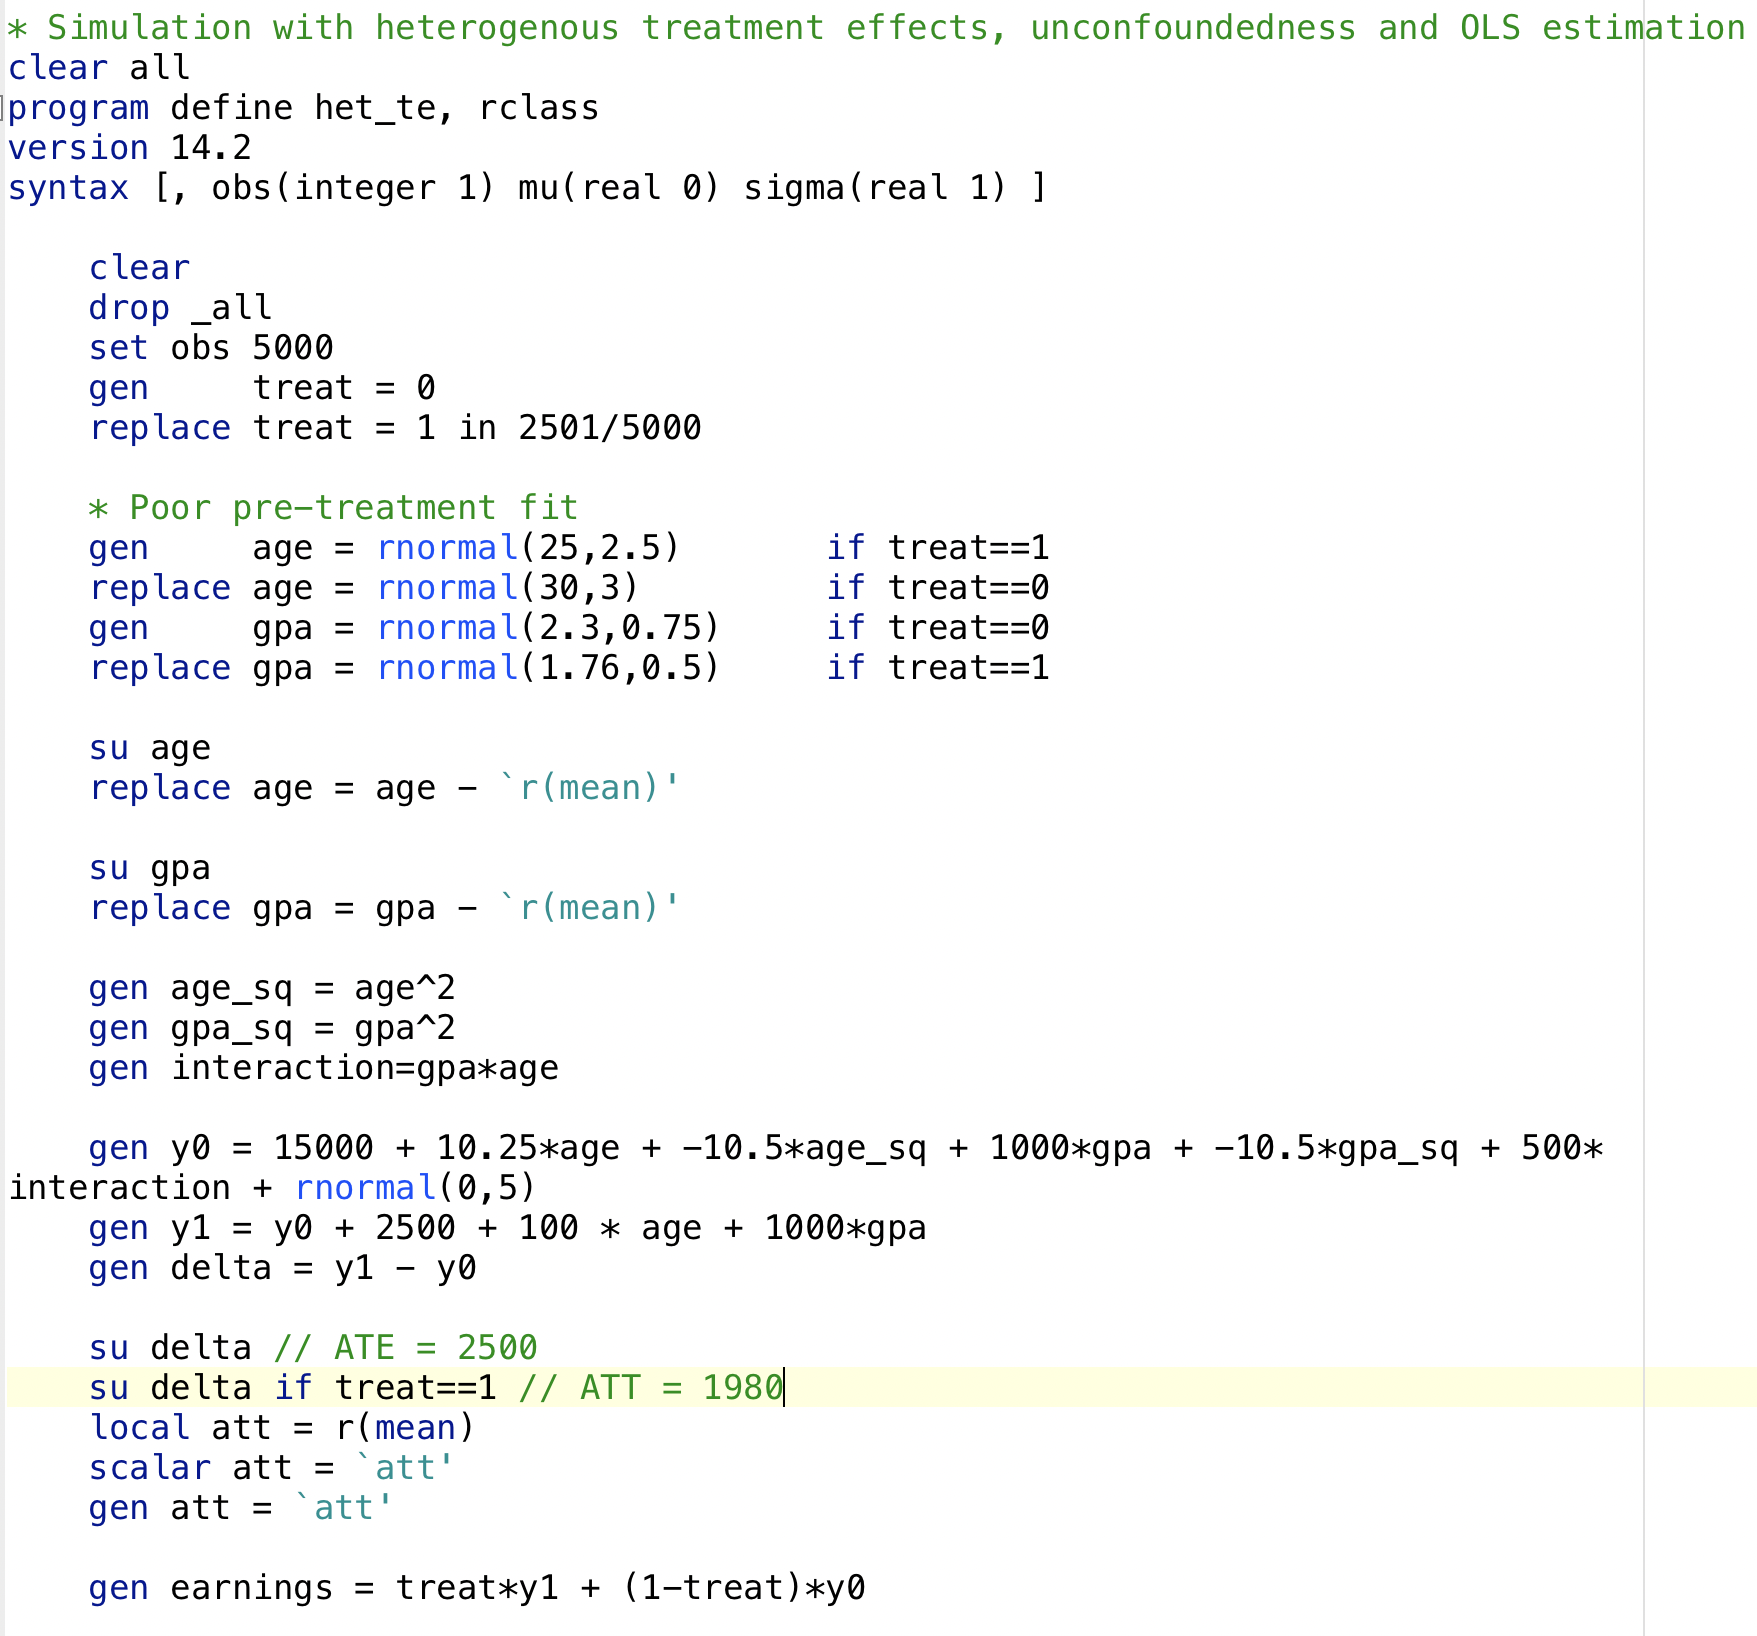
\includegraphics[scale=0.27]{./lecture_includes/stata_matching_code}
\end{figure}

\end{frame}

\begin{frame}{Parameters}

\begin{itemize}

\item We have two parameters: the ATE is \$2500 but the ATT is \$1980
\item What is the specification for each of them?
\item Let's look at what people usually do
\item 1,000 simulations of DGP with regression estimates plotting coefficient on treatment dummy: first with just age and GPA, second with the precise model used for $Y^0$ (but not $Y^1$)

\end{itemize}

\end{frame}


\begin{frame}{Constant Treatment Effects and Linearity}

\begin{figure}[!t]\centering
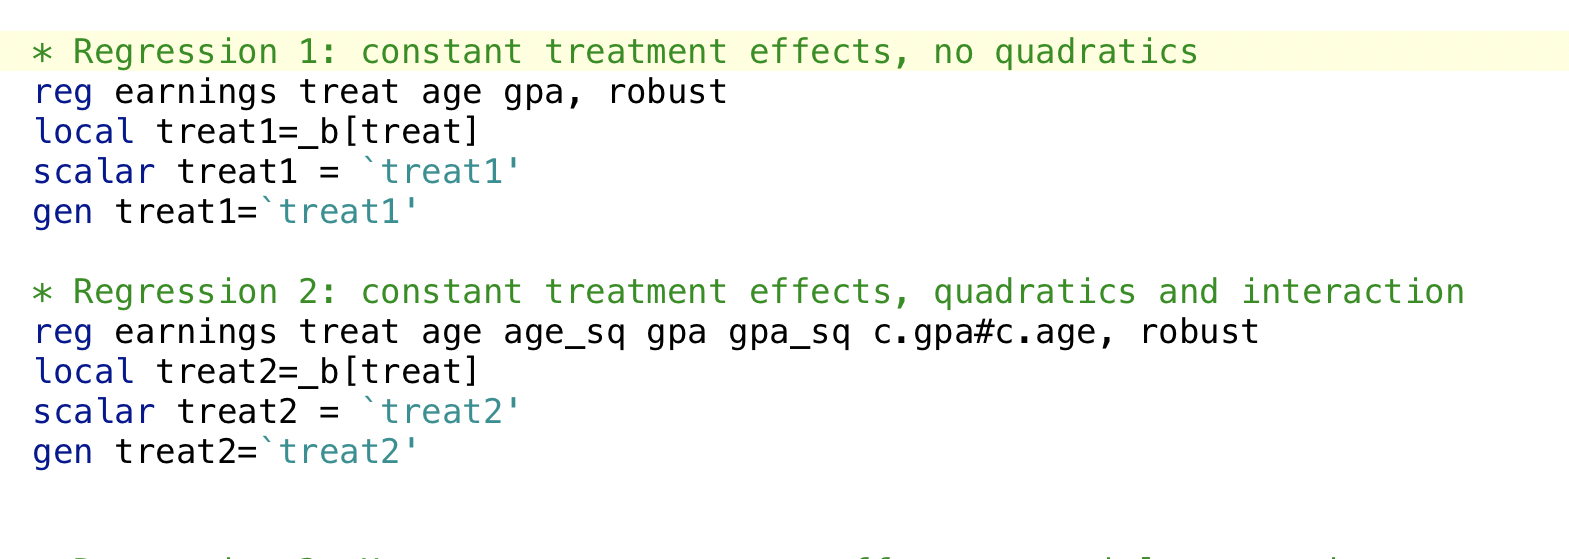
\includegraphics[scale=0.45]{./lecture_includes/stata_reg_constant}
\end{figure}

\end{frame}


\begin{frame}{Coefficient on Treatment Dummy is Wrong}

\begin{figure}[!t]\centering
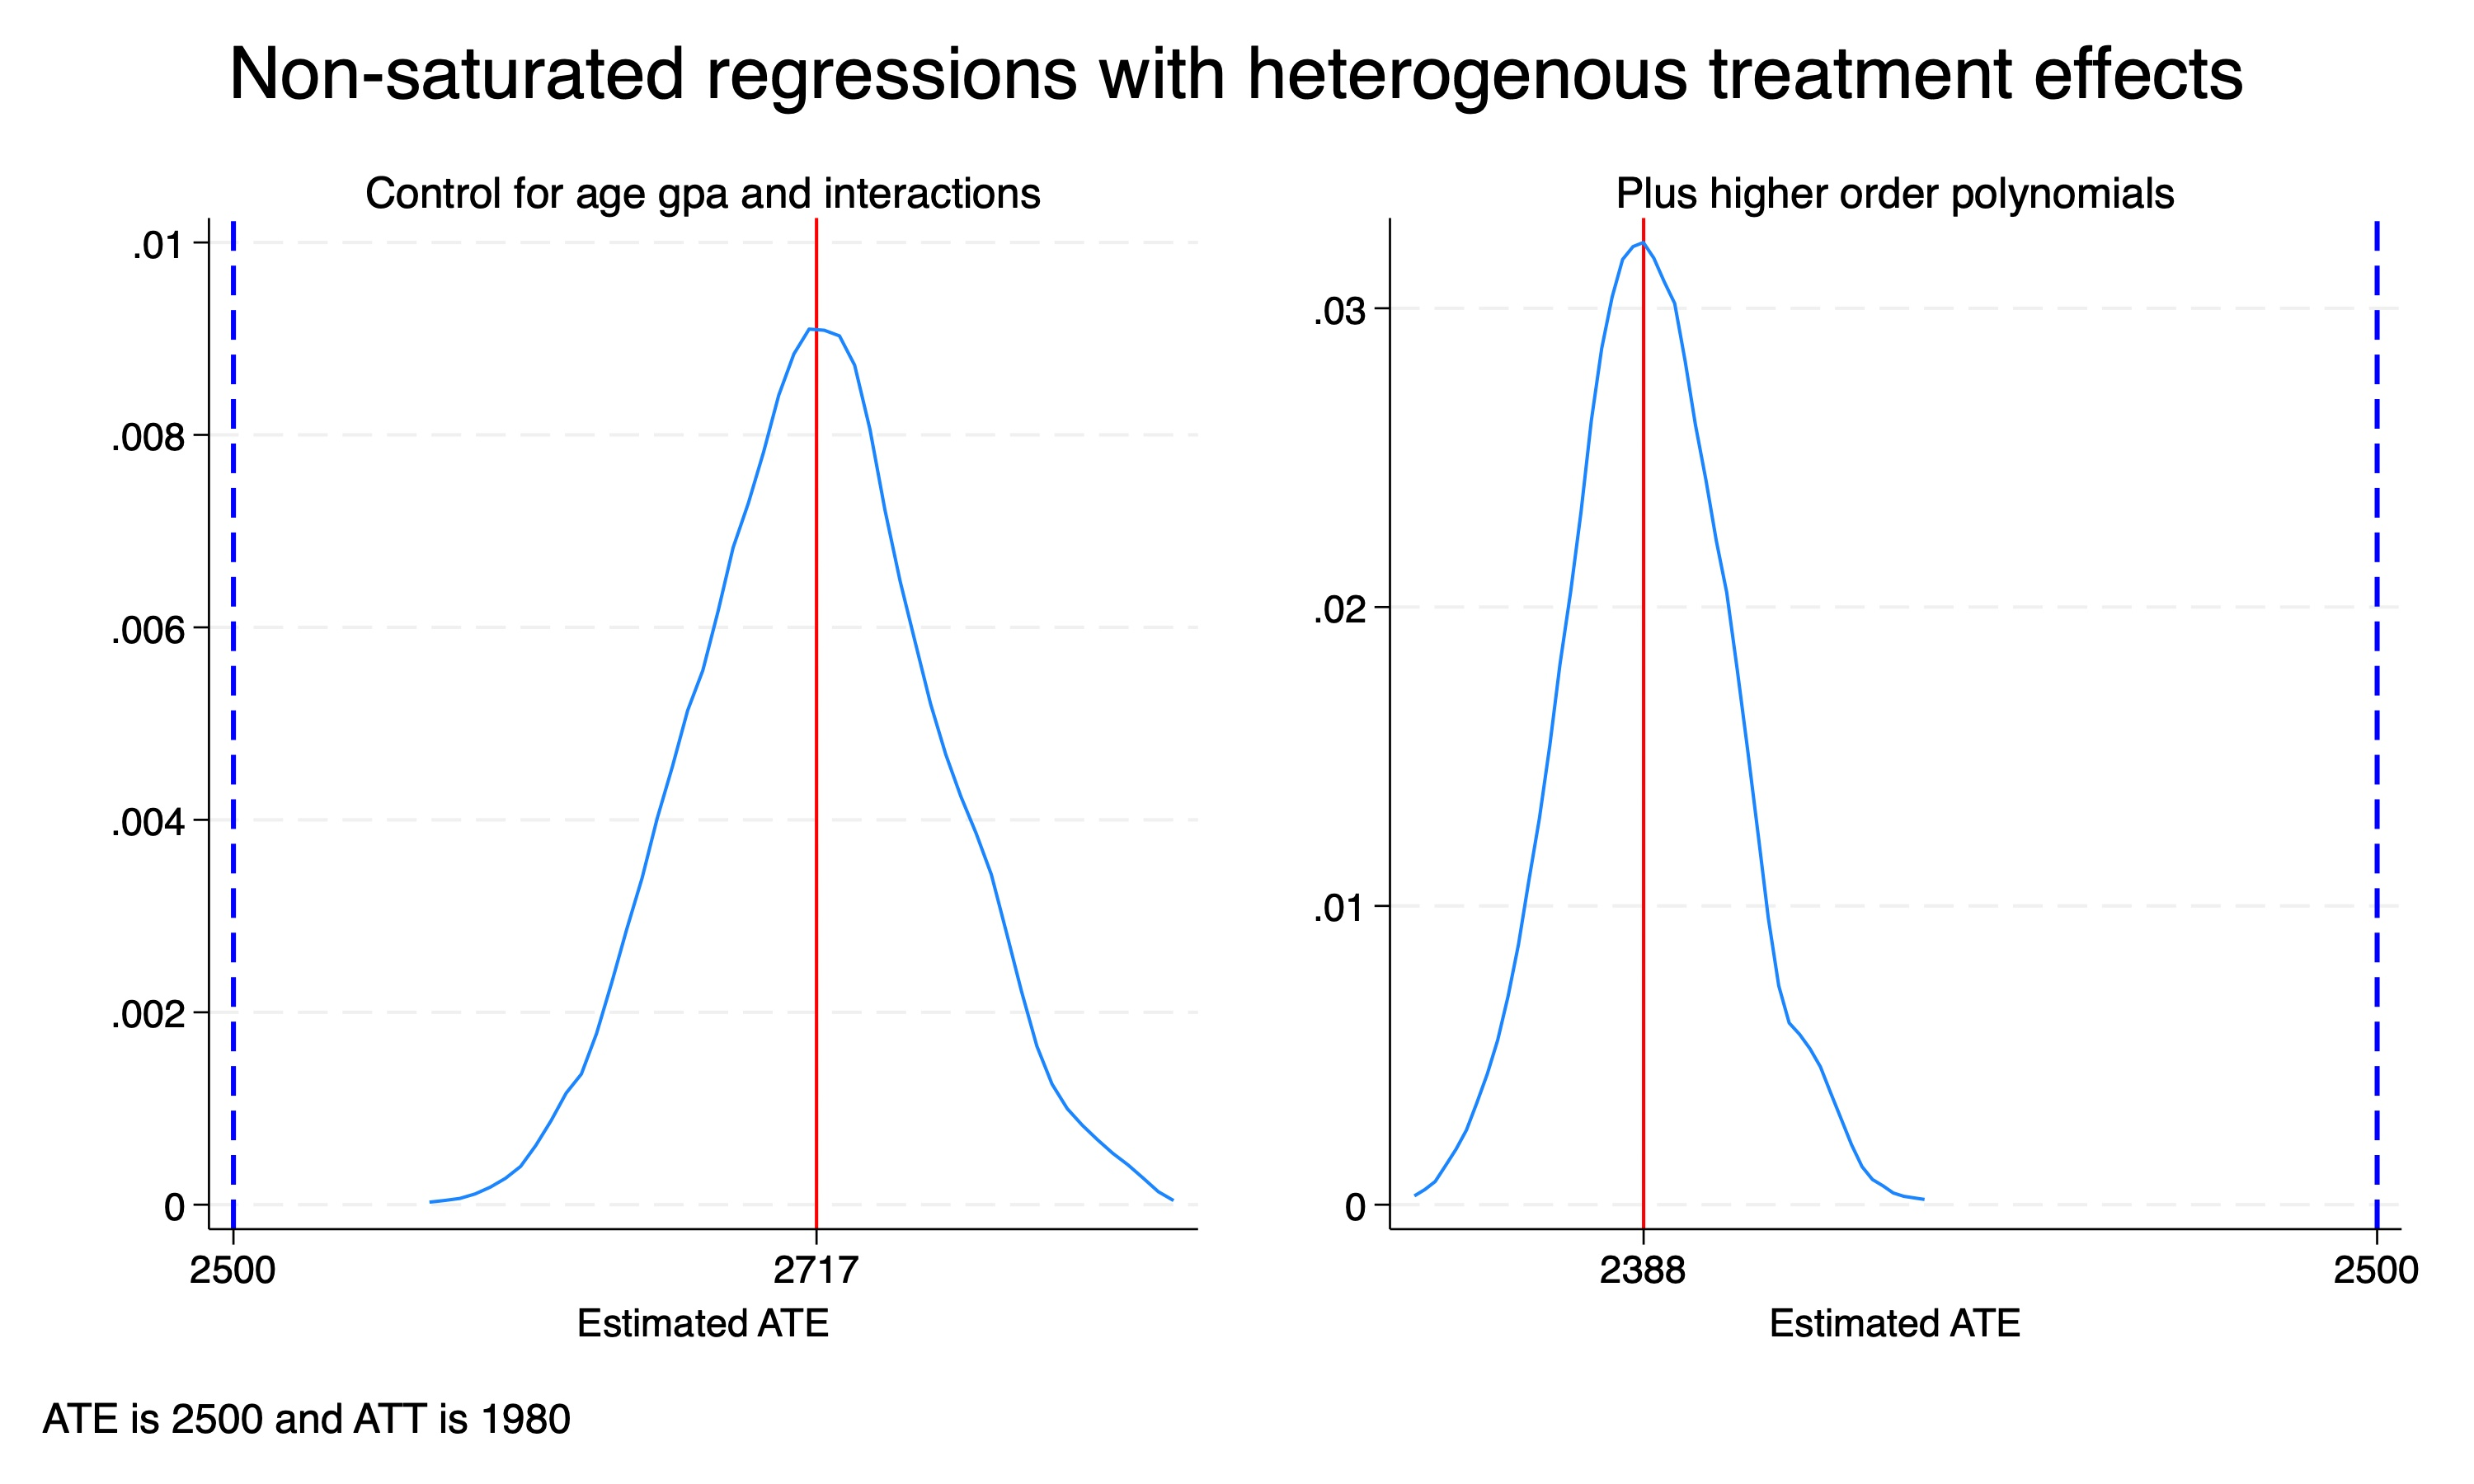
\includegraphics[scale=0.1]{./lecture_includes/combined_kernels.jpg}
\end{figure}

\end{frame}

\begin{frame}{Commentary}

\begin{itemize}

\item Three ifs and a then:

	\begin{itemize}
	\item \emph{If} unconfoundedness held, and 
	\item \emph{if} the potential outcome model was linear, and
	\item  \emph{if} the treatment effect had been homogenous with respect to age and GPA, 
	\item \emph{then} the coefficient on the treatment variable would have been the ATE 
	\end{itemize}
	
\item But it wasn't because homogeneity with respect to $X$ was not true (recall $Y(0)$ coefficients were not the same as $Y(1)$ coefficients)
\item Why were these models biased?  Didn't we have the correct specification in the second graph? 
\end{itemize}

\end{frame}

\begin{frame}{Heterogenous treatment effects}

Write down a simplified version of the DGP from the code:

\begin{eqnarray*}
Y^0_i &=& \alpha + \beta_{01} X_i + \varepsilon_i \\
Y^1_i &=& \alpha + \beta_{01} X_i + \delta D_i + \beta_{11} X_i \times D_i + \varepsilon_i
\end{eqnarray*}

\bigskip

Notice that the setup before, $X_i$ had a different effect on $Y^0$ than it did on $Y_i^1$ -- that's because of heterogenous treatment effects with respect to conditioning set. 

\end{frame}

\begin{frame}{Heterogenous treatment effects}

Take conditional expectations of the \emph{potential} outcomes:

\begin{eqnarray*}
E[Y^0_i | D_i=0, X_i] &=& \alpha + \beta_{01} E[X_i | D_i = 0, X_i] \\
E[Y^1_i | D_i=1, X_i] &=& \alpha + \beta_{01} E[X_i | D_i = 0, X_i]  \\
&& + \delta + \beta_{11} E[X_i | D_i=1,X_i]
\end{eqnarray*}

\bigskip

Average treatment effect is:  $E[Y_i^1 | D_i, X^1_i] - E[Y^0_i | D_i, X_i] $

\bigskip

\footnotesize

\begin{eqnarray*}
&=& \bigg (  \alpha + \beta_{01} E[X_i | D_i=0, X_i] + \delta + \beta_{11} E[X_i \times D_i | D_i=1,X_i] \bigg ) \\
&& -  \bigg (\alpha + \beta_{01} E[X_i  | D_i=0, X_i] \bigg ) \\
&=& \delta + \beta_{11}  E[X_i \times D_i | D_i=1] 
\end{eqnarray*}OLS model accounting for heterogeneity must be ``fully saturated''.


\end{frame}




\begin{frame}{Regression adjustment}

This implies an interacted OLS model or what Wooldridge (2010) calls regression adjustment:

\bigskip

\begin{eqnarray*}
Y_i = \alpha + \delta D_i + \beta_{01} X_i + \beta_{11} D_i \times X_i + \varepsilon_i
\end{eqnarray*}

$\widehat{\delta}$ is the ATE but the ATT is equal to $\widehat{\delta} + \widehat{\beta_{11}} E[X_i | D_i = 1]$ where $E[X_i | D_i=1]$ is the sample average of $X_i$ for the treatment group

\bigskip

We will estimate two models: (1) once with simplified but incorrectly specified saturated and (2) another with the correctly specified saturated model -- warning, it's a huge pain and you can easily mess it up even with just a few variables

\end{frame}



\begin{frame}{Misspecified Saturated OLS Regression}

\begin{figure}[!t]\centering
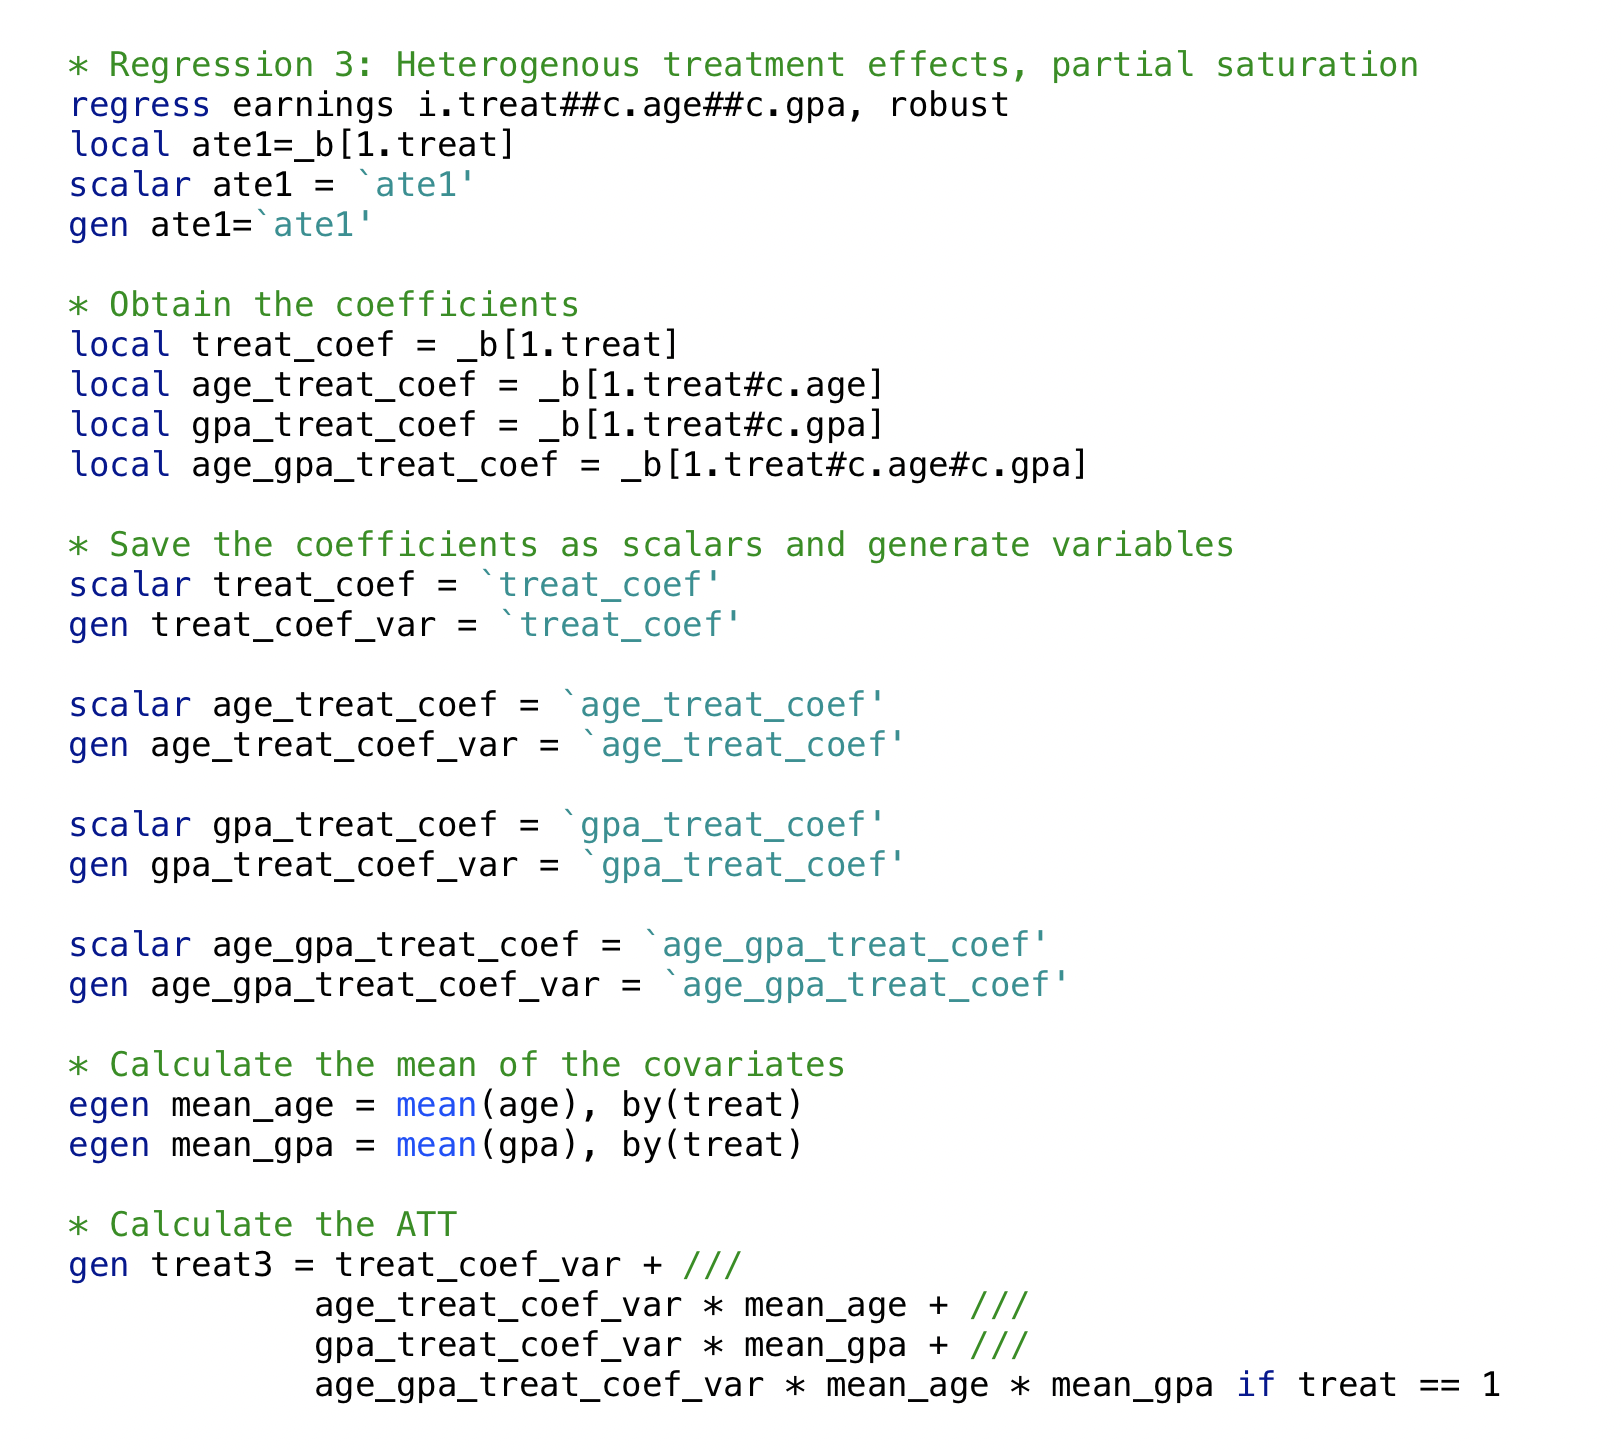
\includegraphics[scale=0.3]{./lecture_includes/saturated_reg3}
\end{figure}

\end{frame}


\begin{frame}{Misspecified Saturated OLS Regression}

\begin{figure}[!t]\centering
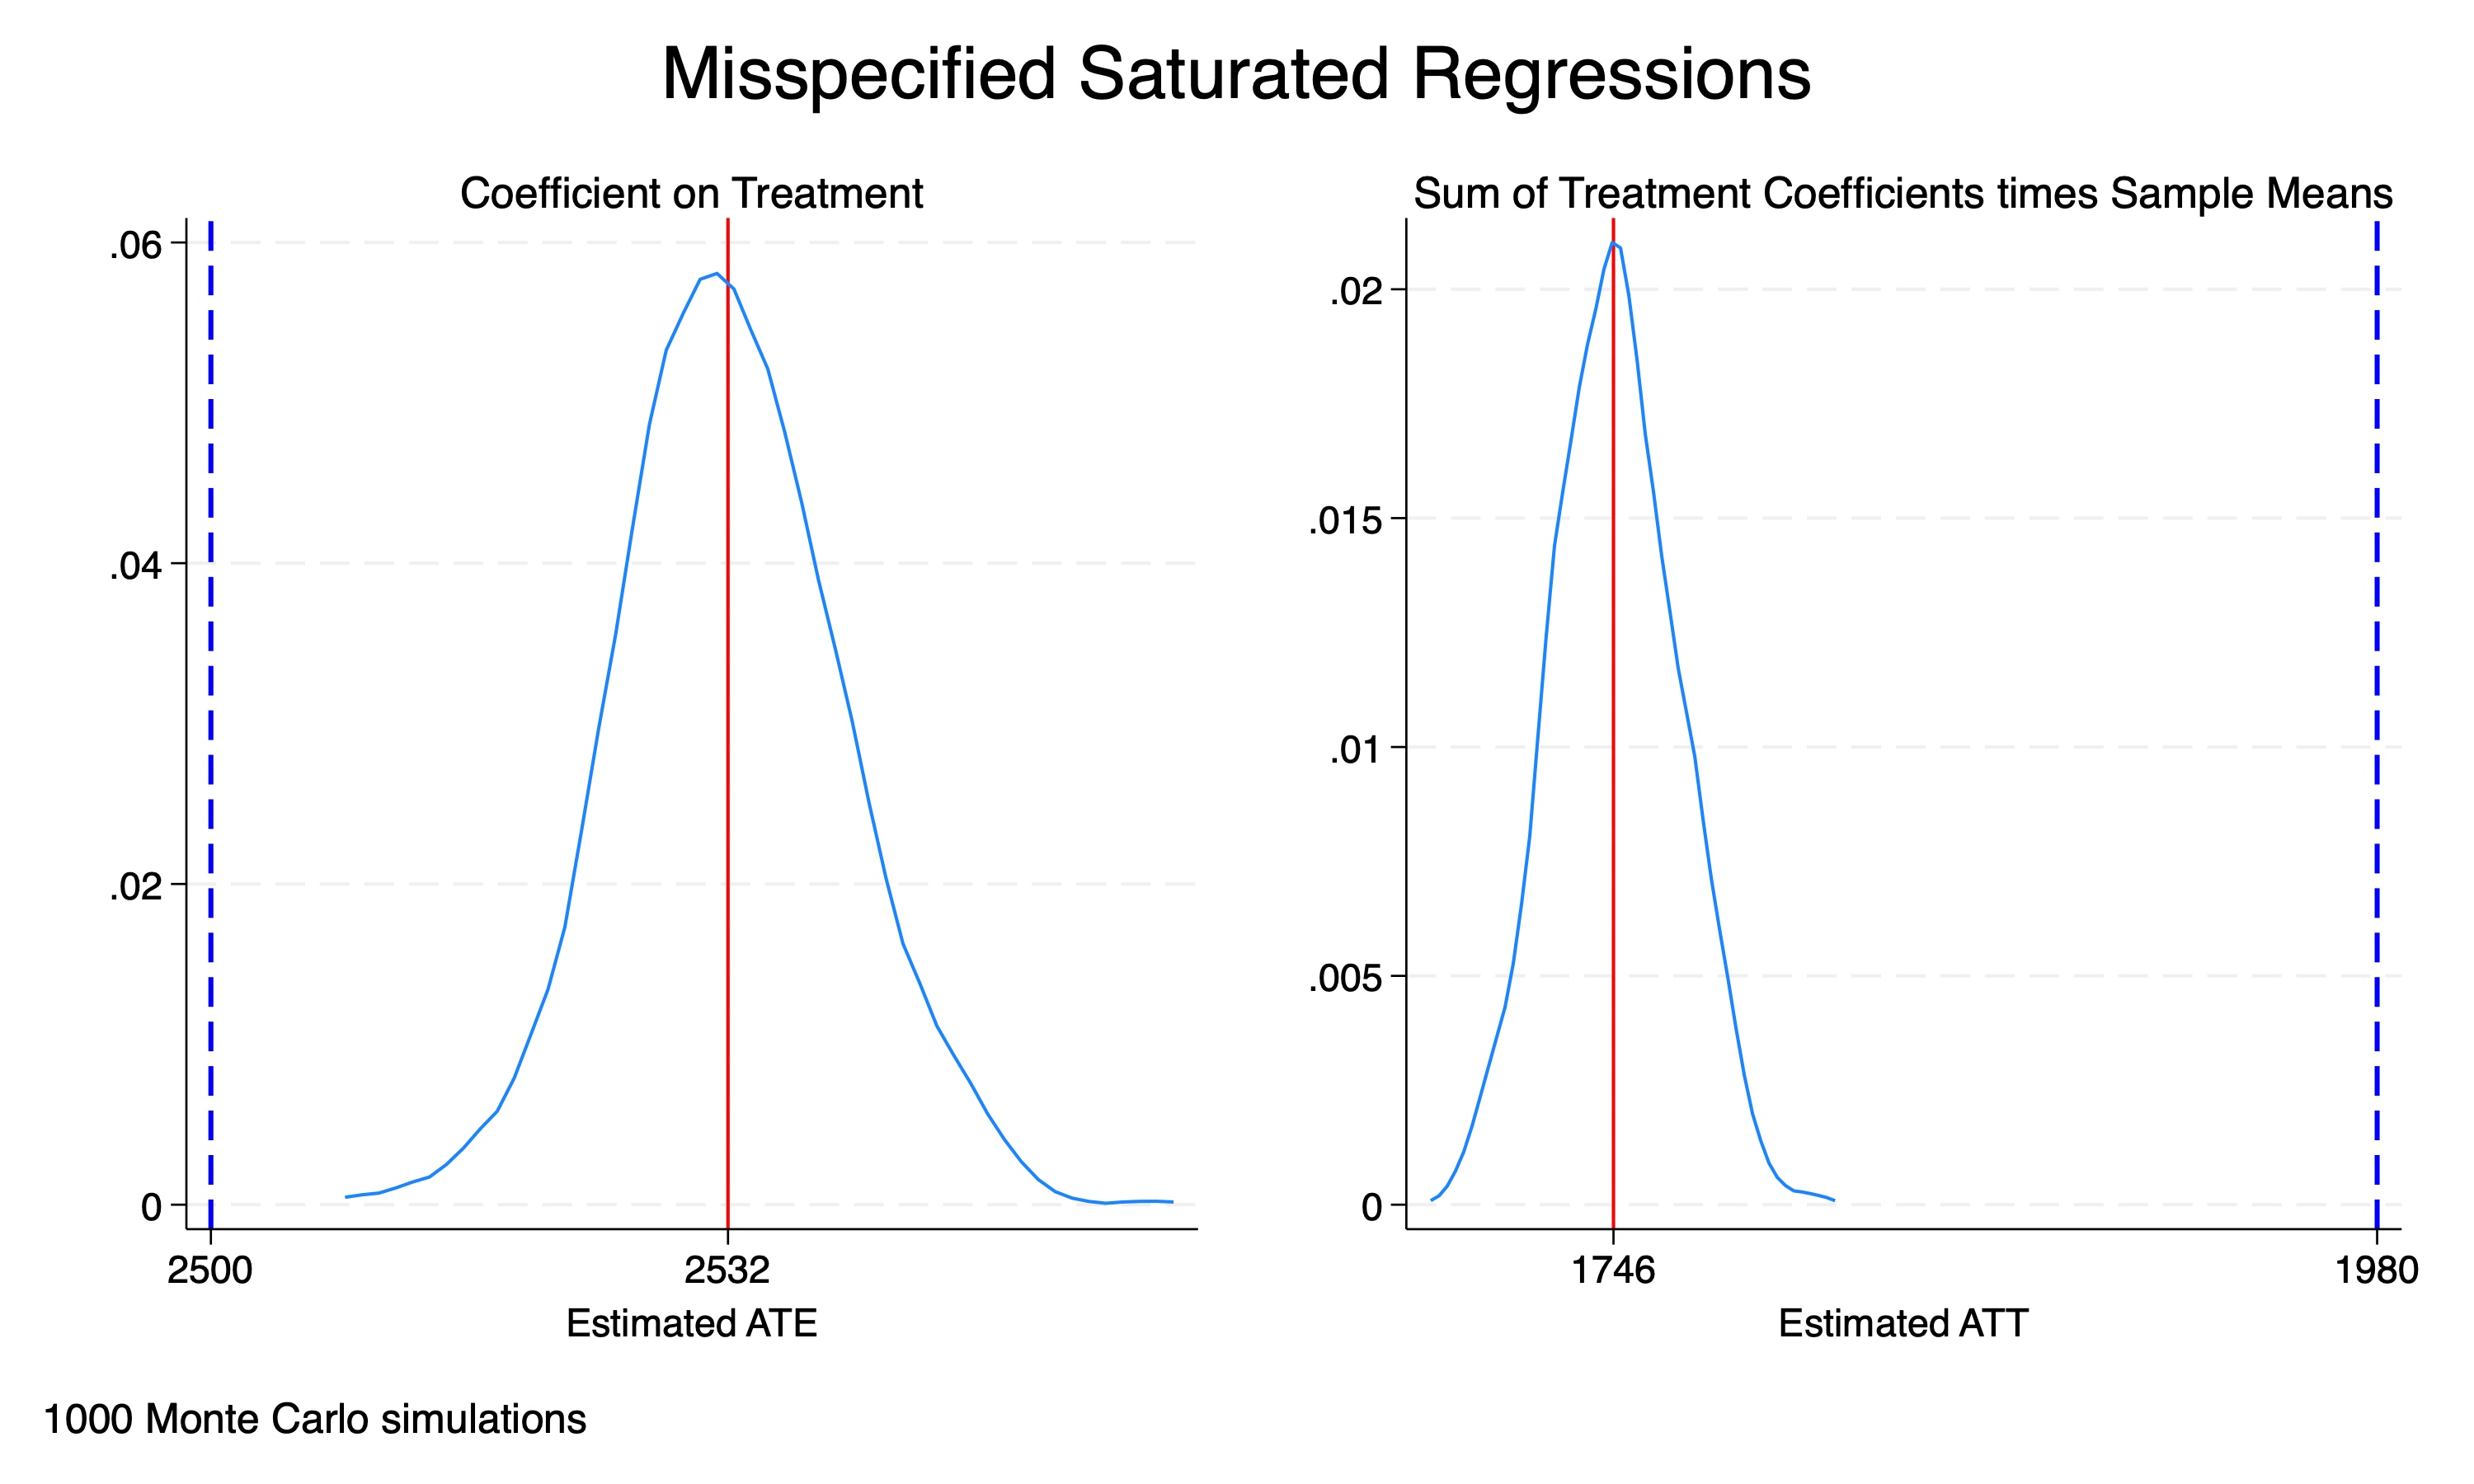
\includegraphics[scale=0.1]{./lecture_includes/combined_saturated1.jpg}
\end{figure}

\end{frame}

\begin{frame}{Comically Long Saturated OLS Regression}

\begin{figure}[!t]\centering
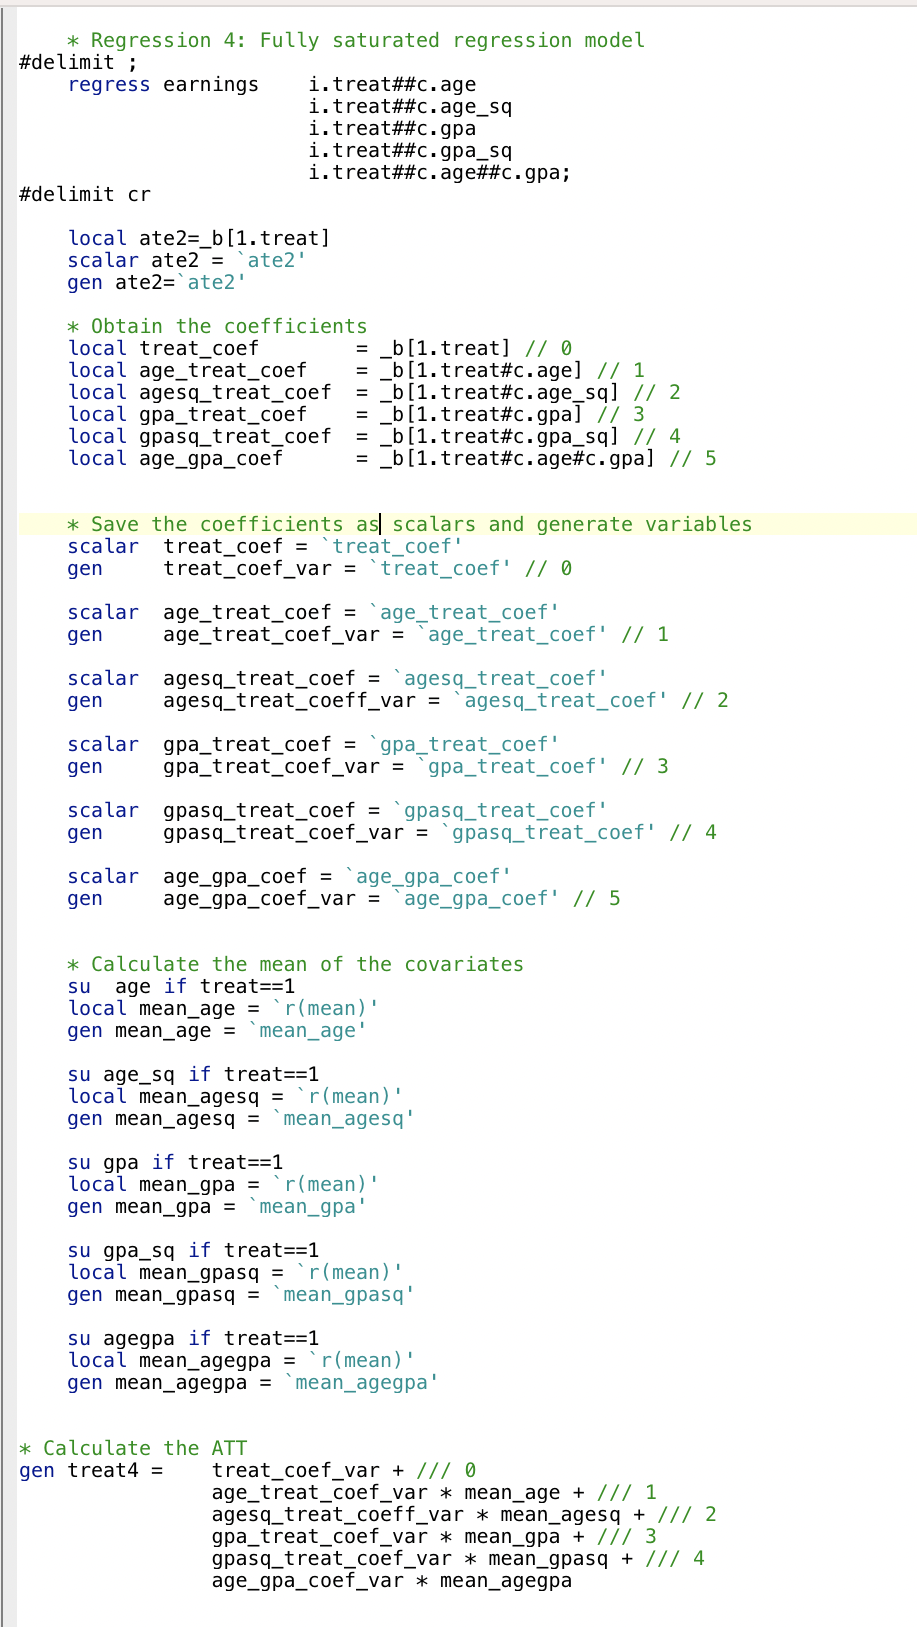
\includegraphics[scale=0.26]{./lecture_includes/stata_full_code}
\end{figure}

\end{frame}

\begin{frame}{Correctly Saturated OLS Regression}

\begin{figure}[!t]\centering
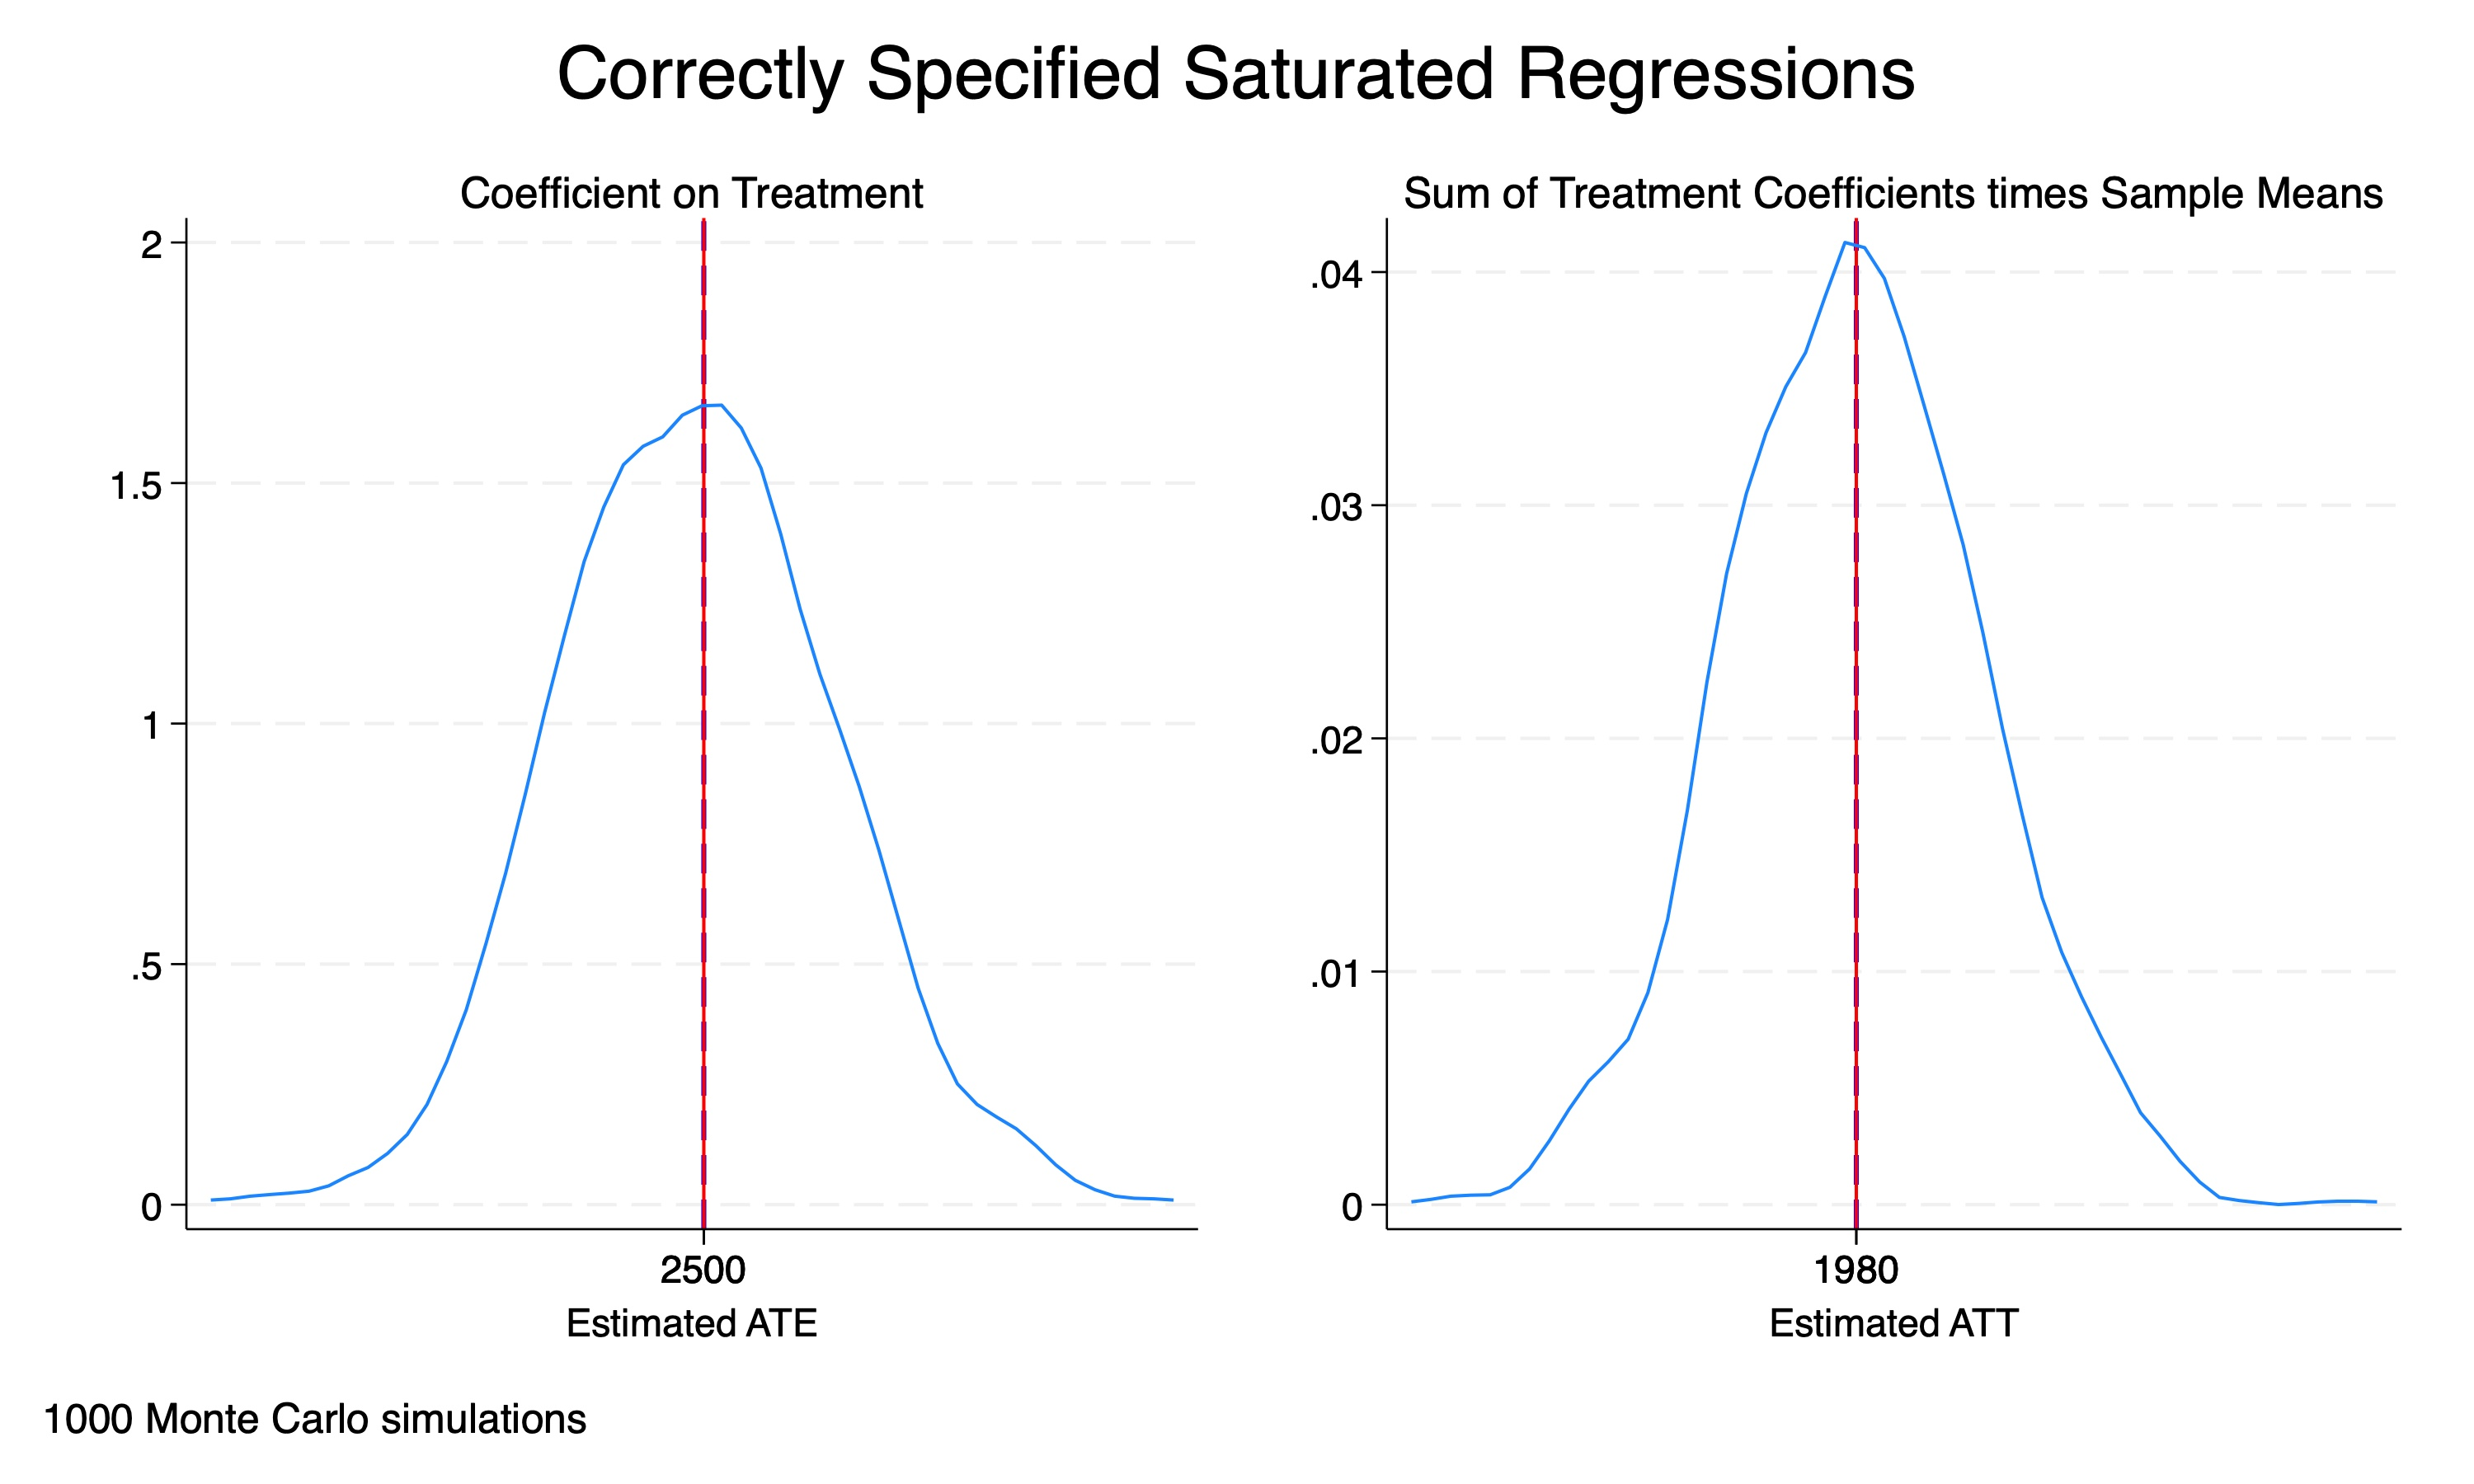
\includegraphics[scale=0.1]{./lecture_includes/combined_saturated2.jpg}
\end{figure}

\end{frame}

\begin{frame}{Regression adjustment}

\begin{itemize}

\item Notice how the same regression (fully interacted) led to \emph{both} the ATE and the ATT?
\item That means if you don't state ahead of time which parameter you want, how are you going to know how to set it up, and how will you know how to recover it?
\item Thankfully software exists that does this for you called ``regression adjustment'' by Wooldridge (2010) or Oaxaca-Blinder (Kline 2011; Graham and Pinto 2022) 
\item In Stata teffects, you can just the \texttt{ra} to get it -- see \texttt{comparison.do}

\end{itemize}

\end{frame}

\begin{frame}{Great quote}

\begin{quote}
``OLS is \dots the linear projection of Y on D and X [and] provides the best linear predictor of Y given D and X (Angrist and Pishcke 2009).  However, if our goal is to conduct causal inference, then this is not, in fact, a good reason to use this method.  OLS is `best' in predicting actual outcomes, but causal inference is about predicting [fictional potential] outcomes.  \dots In other words, OLS \dots is optimal for predicting `what is'.  Instead we are interested in predicting `what would be' if treatment were assigned differently.'' - Tymon Sloczynski, Restat 2022
\end{quote}

\end{frame}


\begin{frame}{Matching}

\begin{itemize}

\item Now let's estimate the ATT (\$1980) using nearest neighbor matching by minimizing Mahalanobis distance on age, GPA, polynomials and interaction
\item One line in Stata using \texttt{teffects} and only 1 match (variance is simple to estimate until we use matches multiple times, then the variance grows)
\item In R, the package is \texttt{Matching}, not sure in python
\end{itemize}

\end{frame}


\begin{frame}{Matching Estimation}

\begin{figure}[!t]\centering
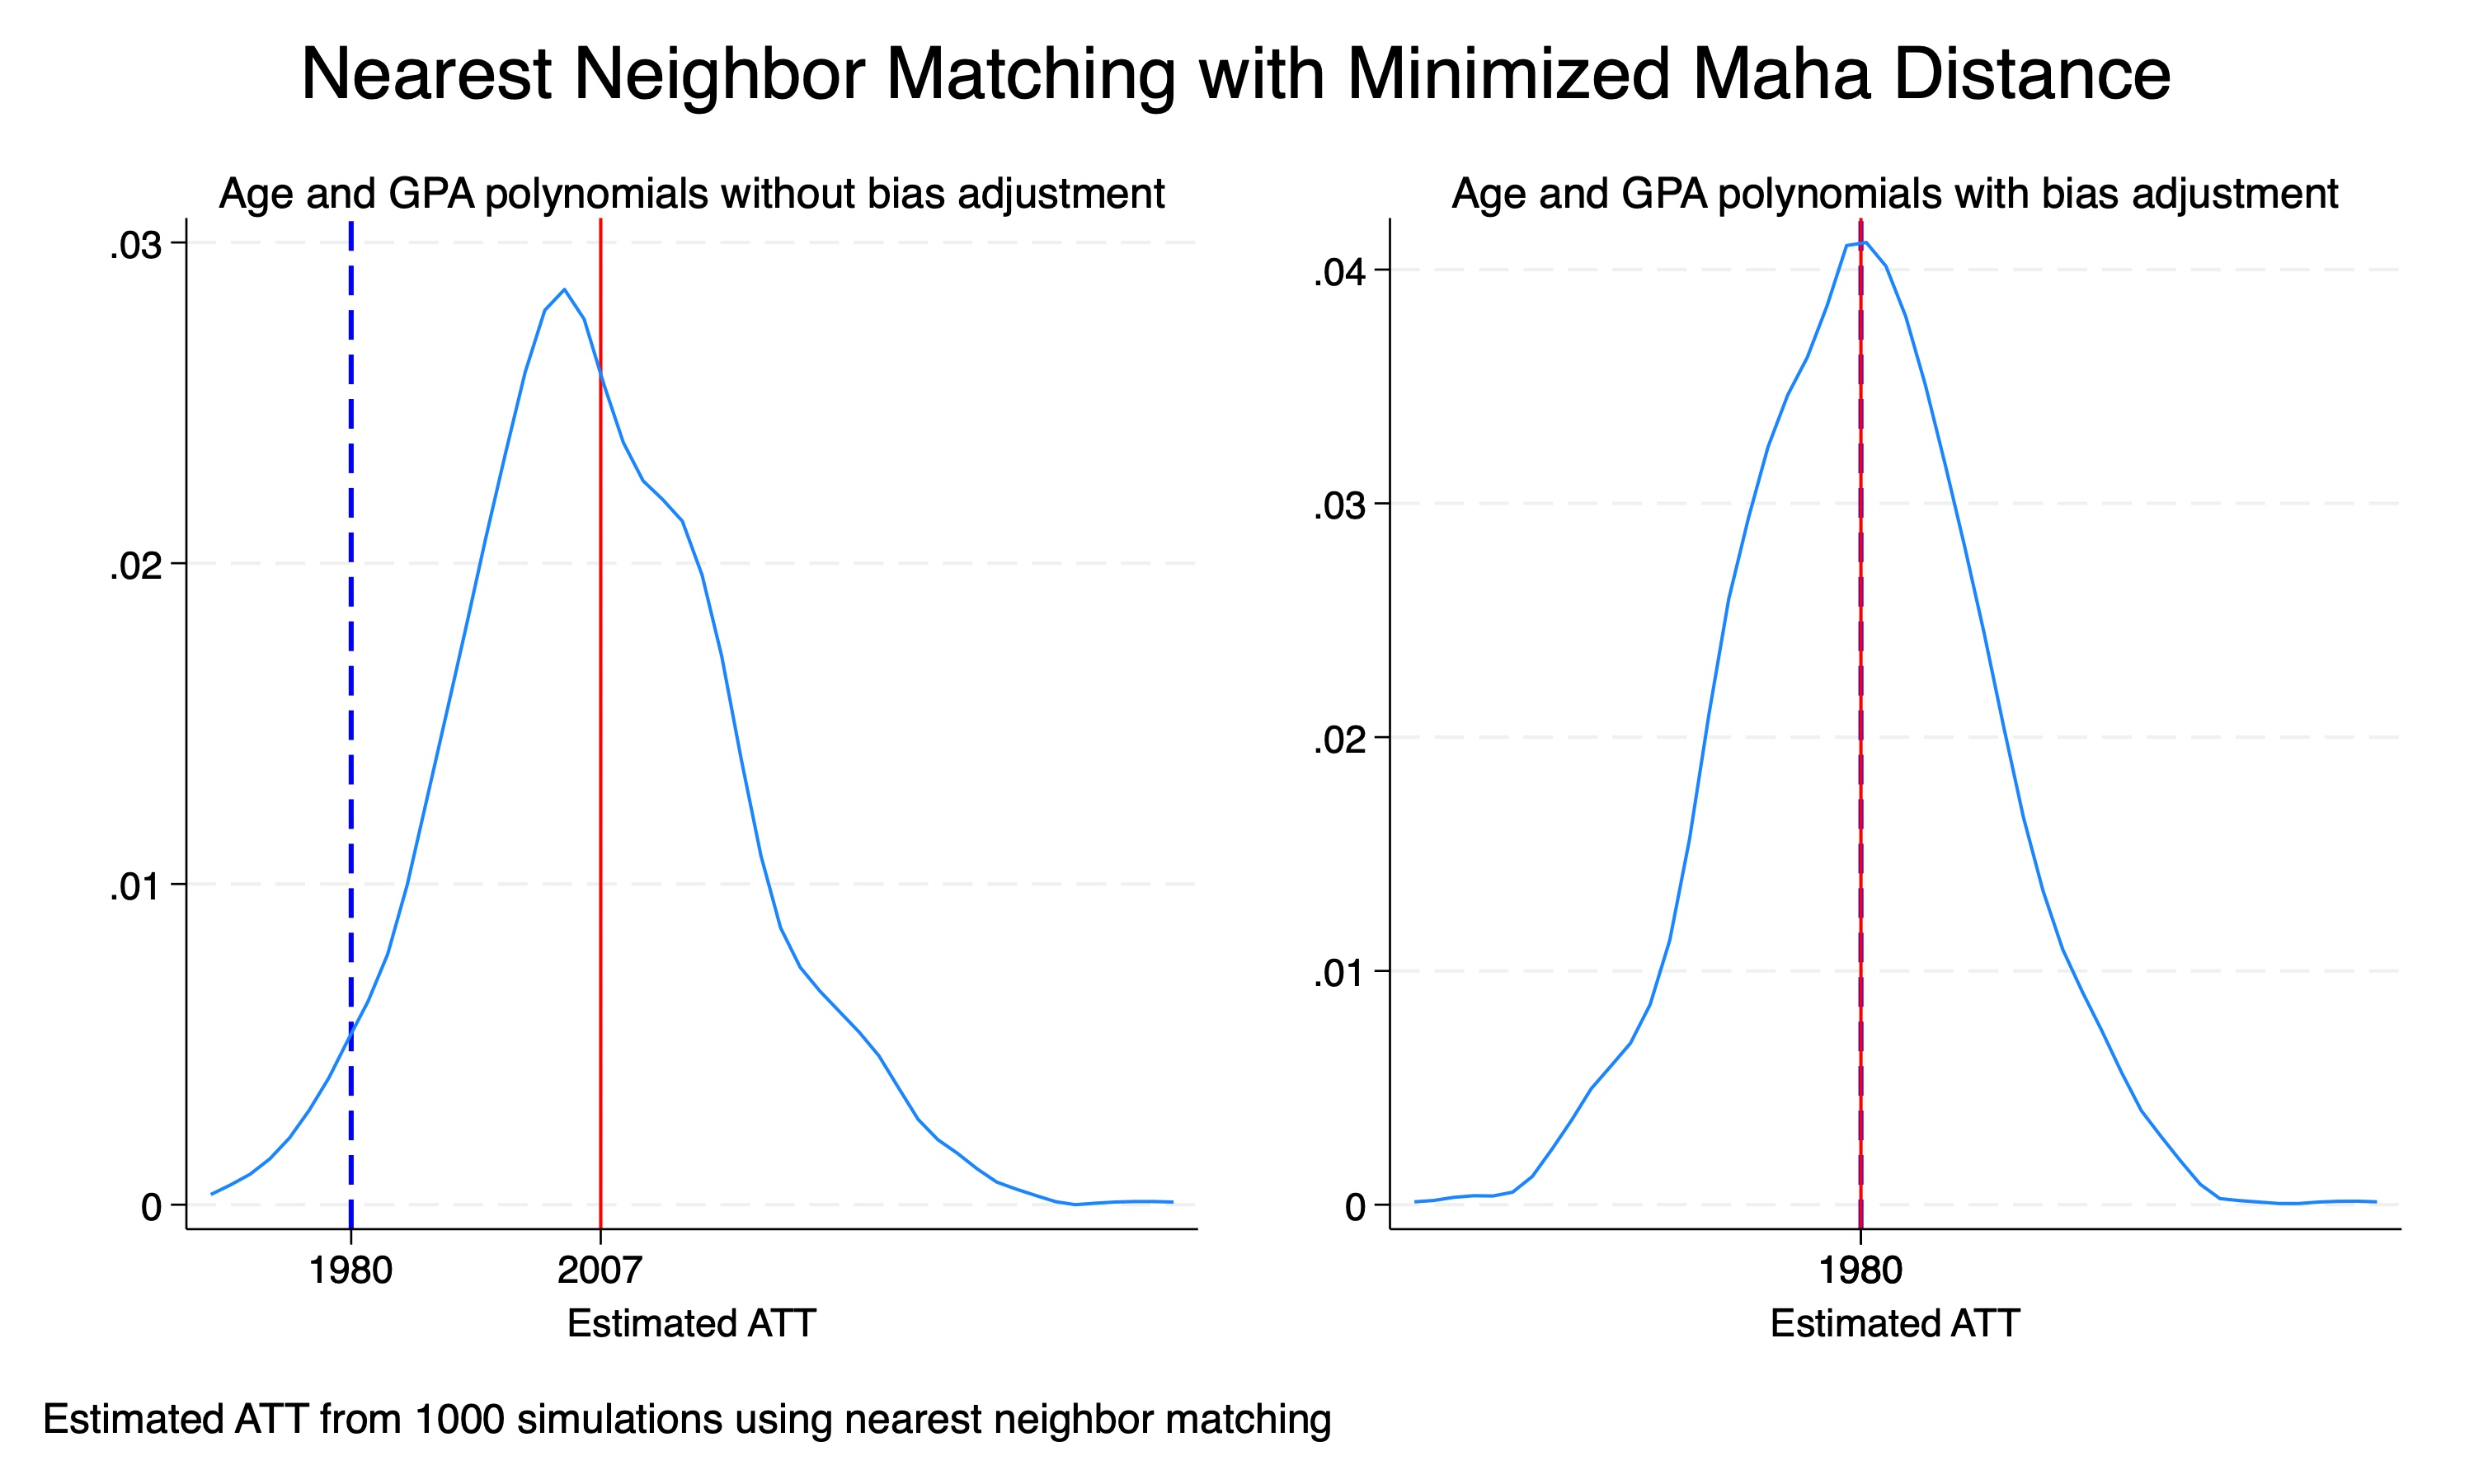
\includegraphics[scale=0.1]{./lecture_includes/combined_kernels_maha.jpg}
\end{figure}

\end{frame}

\begin{frame}{Commentary}

\begin{itemize}

\item Technically I was only ``fully interacting'' -- full saturation would be to interact the treatment dummy with every value of the covariates yielding a huge number of parameters likely that cannot be estimated
\item Regression adjustment within -teffects- will do this for you
\item But note, with heterogeneity you have to use the fully saturated model (I just hadn't dummied every value of the covariates) to get both the ATE and the ATT
\item Otherwise you are imposing strong and unnecessary assumptions on the data that the treatment effects are the same for all values of $X$ and constant treatment effects so that the single coefficient is the ATE and the ATT

\end{itemize}

\end{frame}

\begin{frame}{Misspecified functional form regression visual}

  \begin{figure}
    
\includegraphics[scale=0.17]{./lecture_includes/regression_linearity.png}
  \end{figure}
  
Using our medieval castle example, if you have the wrong functional form, then regression won't hit.

\end{frame}


\begin{frame}{Nonlinear DGP}

\begin{itemize}

\item We've seen what happens if there's heterogenous treatment effects with respect to covariates
\item But this was resolvable with ``full interaction'' or ``regression adjustment''
\item But Imbens and Rubin (2015) noted that exogeneity also implied functional forms, namely linearity
\item Let's examine this now using a very unusual DGP using \texttt{nonlinear\_matching.do}

\end{itemize}

\end{frame}




\begin{frame}{Nonlinear DGP}

\begin{figure}[!t]\centering
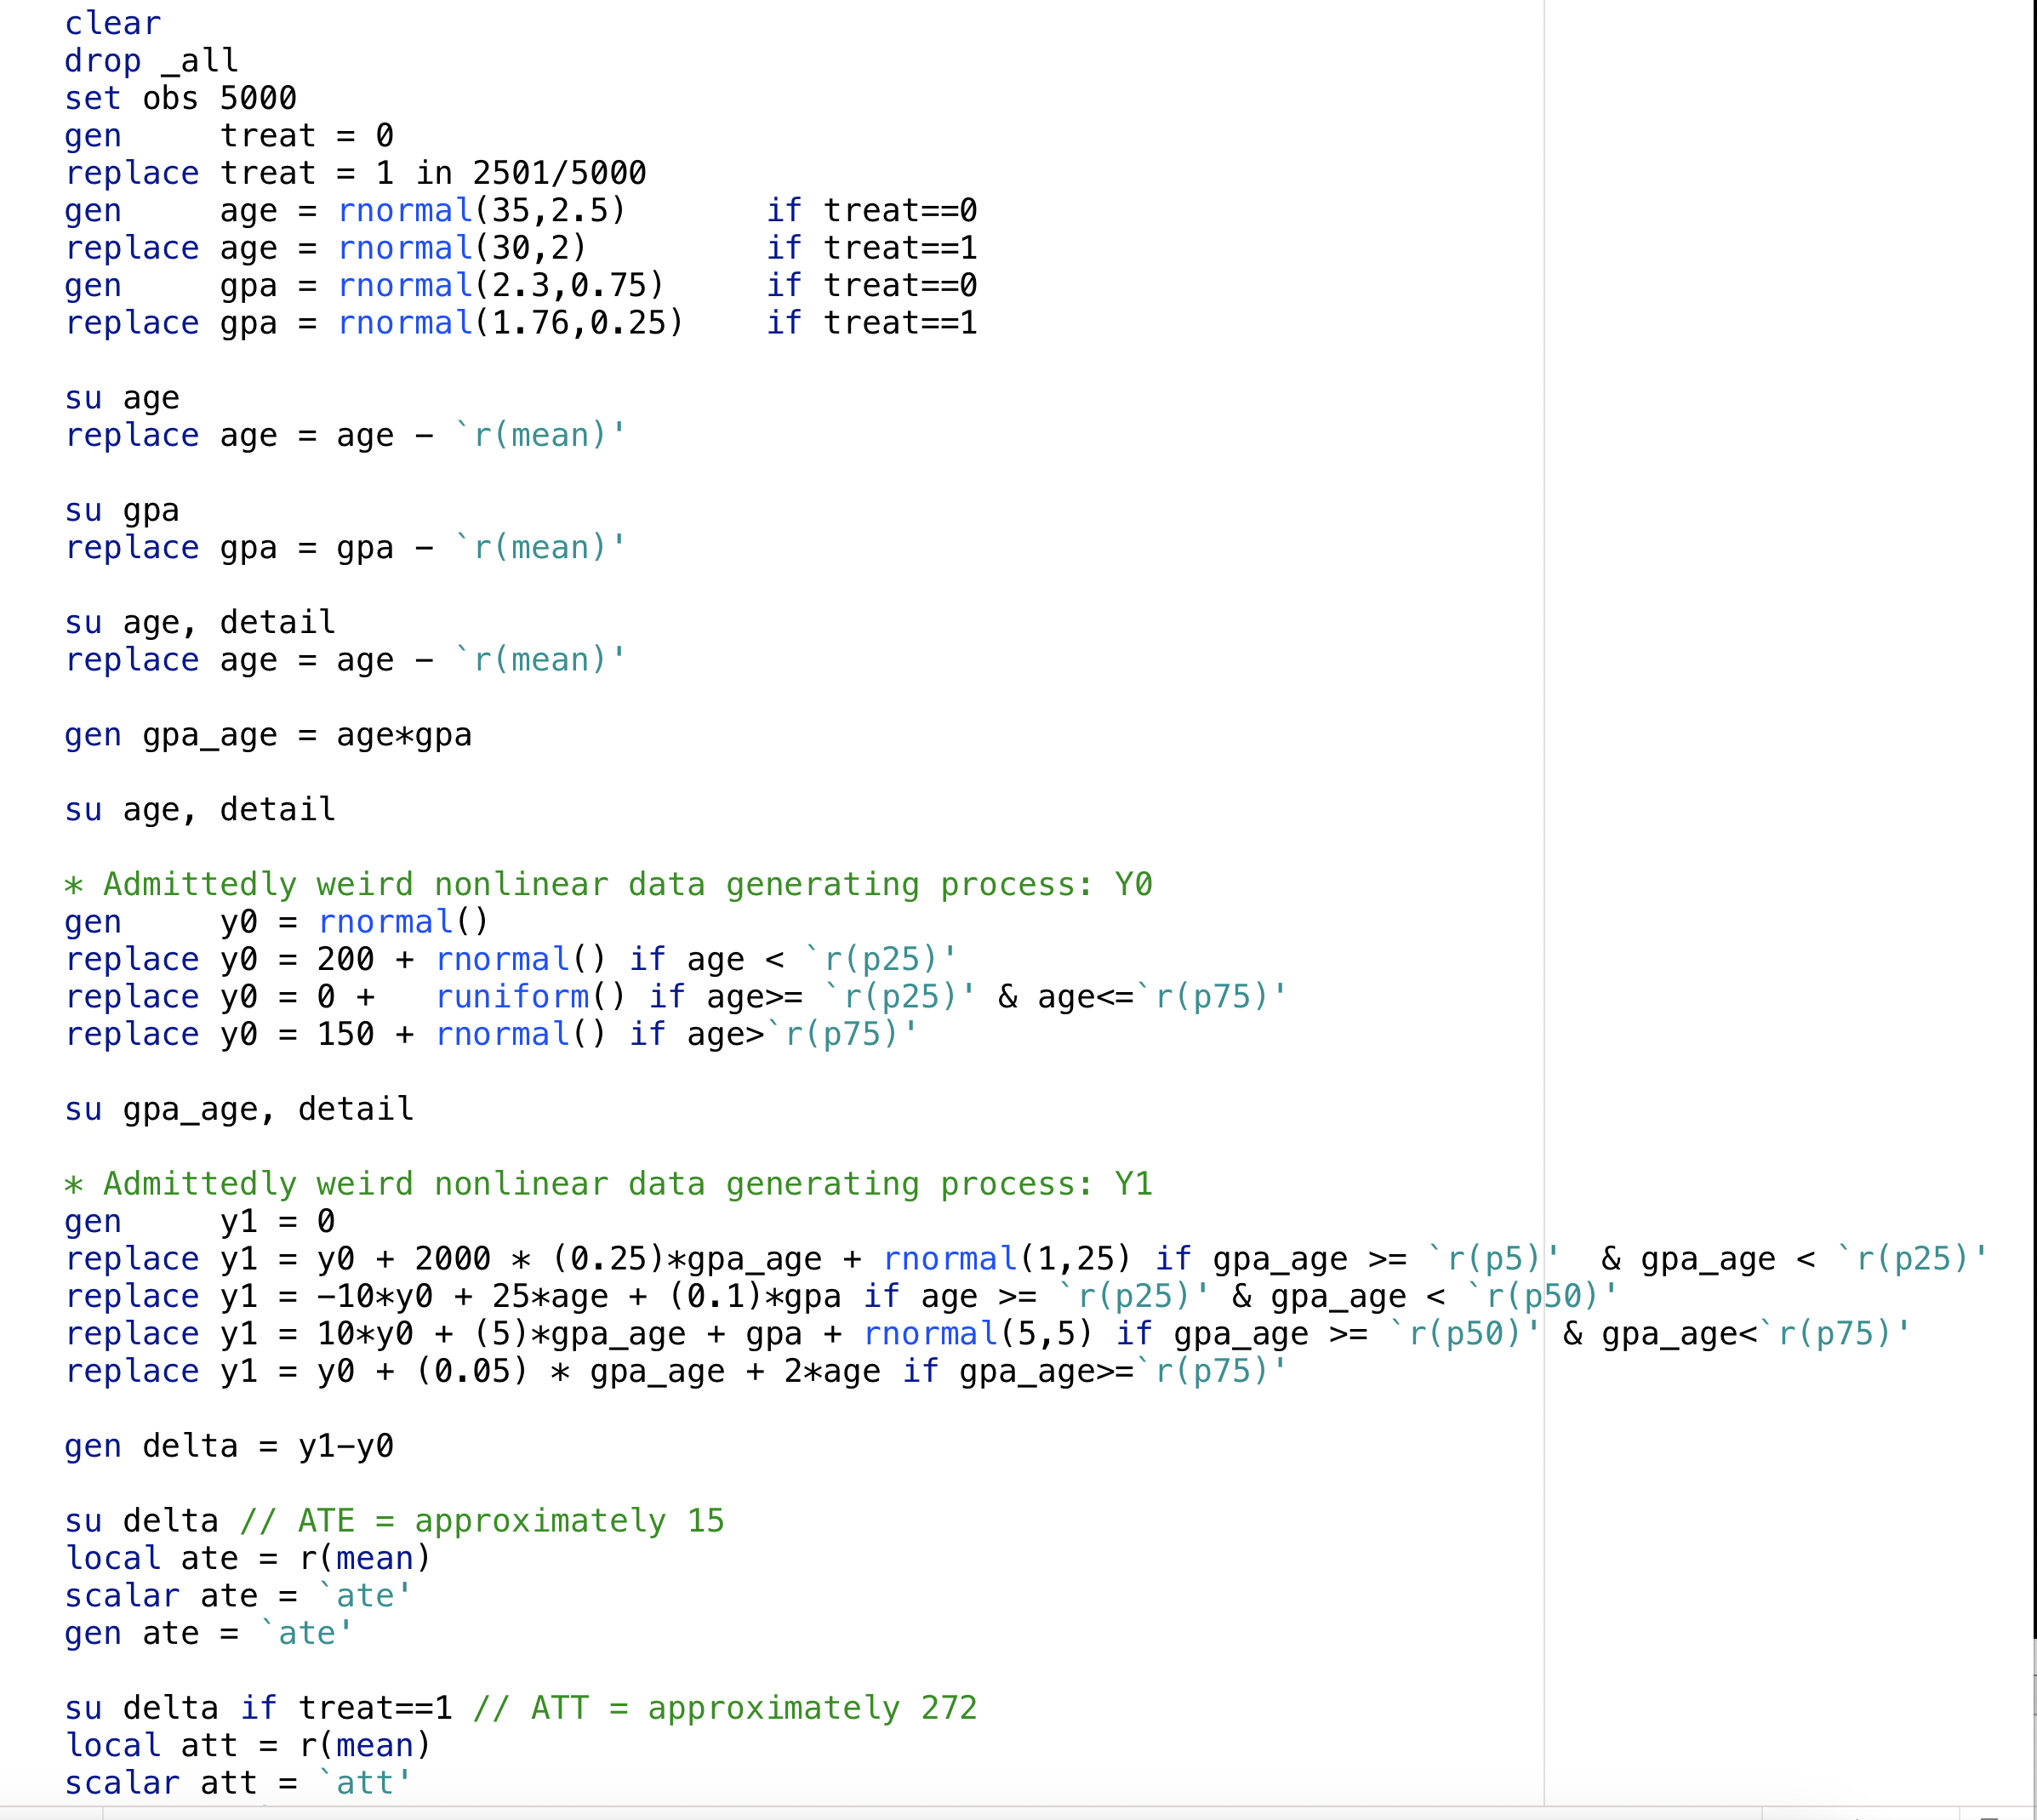
\includegraphics[scale=0.21]{./lecture_includes/nonlinear_code}
\end{figure}

\end{frame}

\begin{frame}{Nonlinear DGP, OLS with RA}

\begin{figure}[!t]\centering
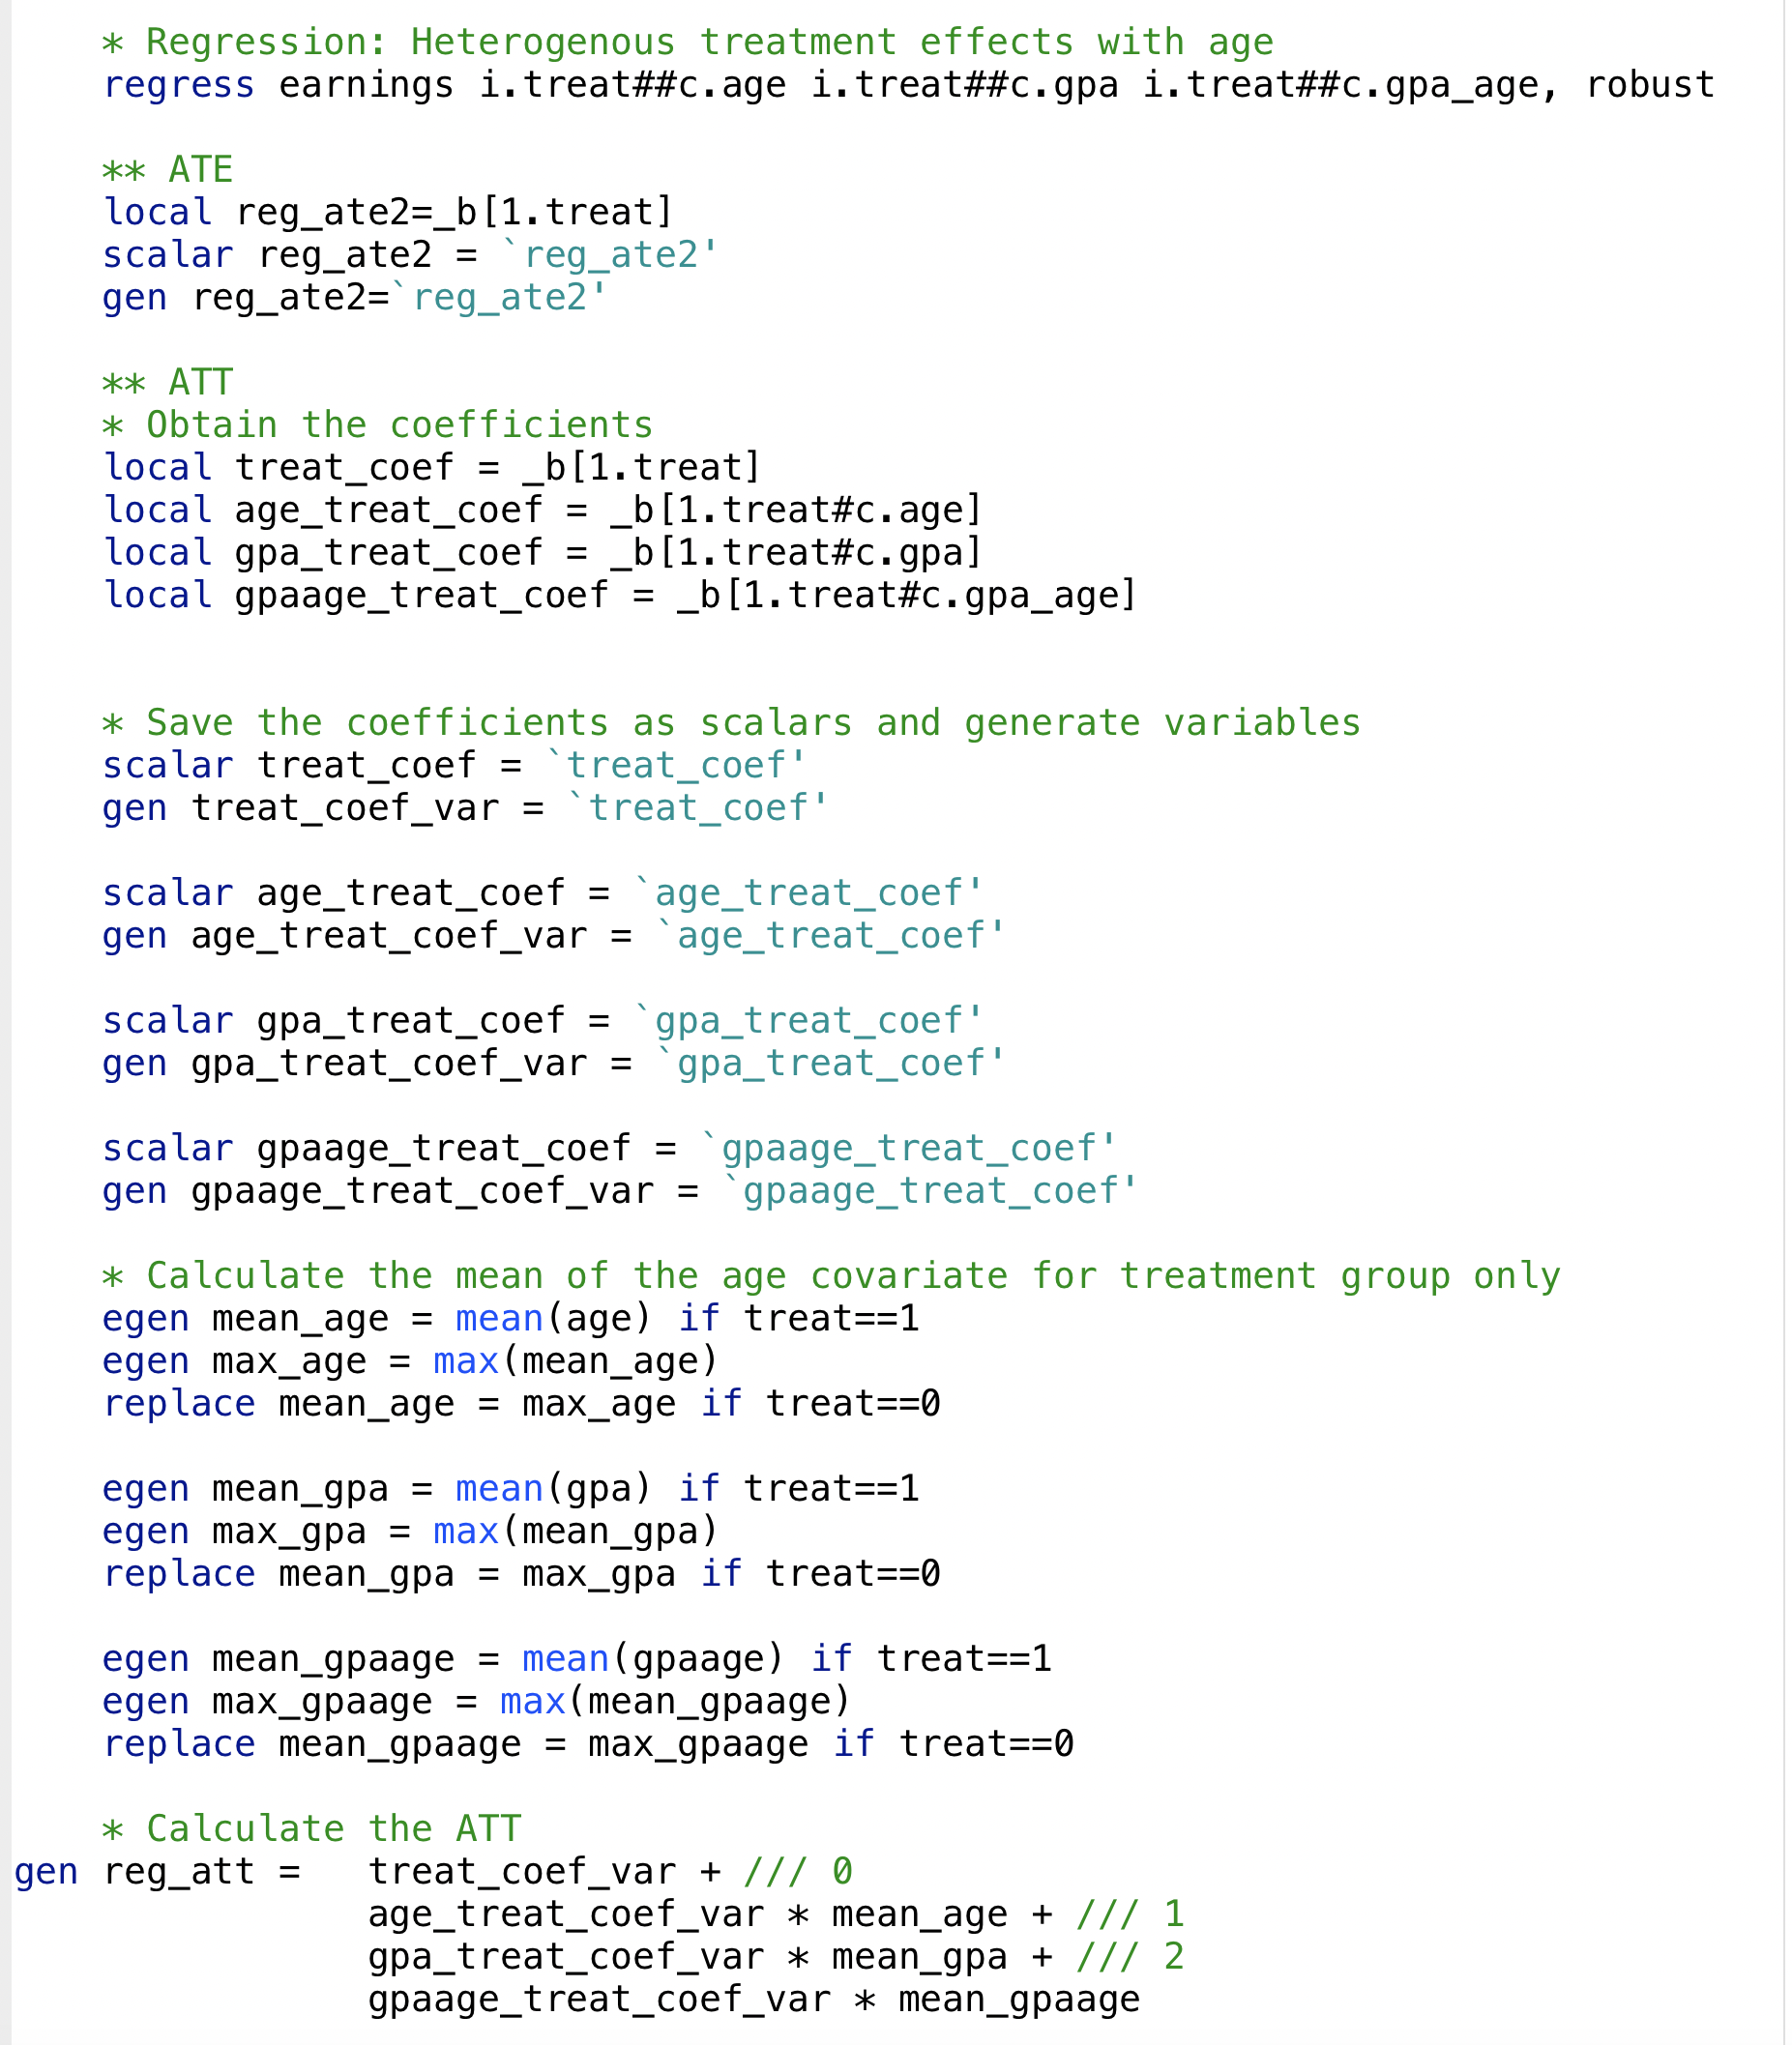
\includegraphics[scale=0.21]{./lecture_includes/nonlinear_ra}
\end{figure}

\end{frame}


\begin{frame}{Nonlinear DGP and Matching}

\begin{figure}[!t]\centering
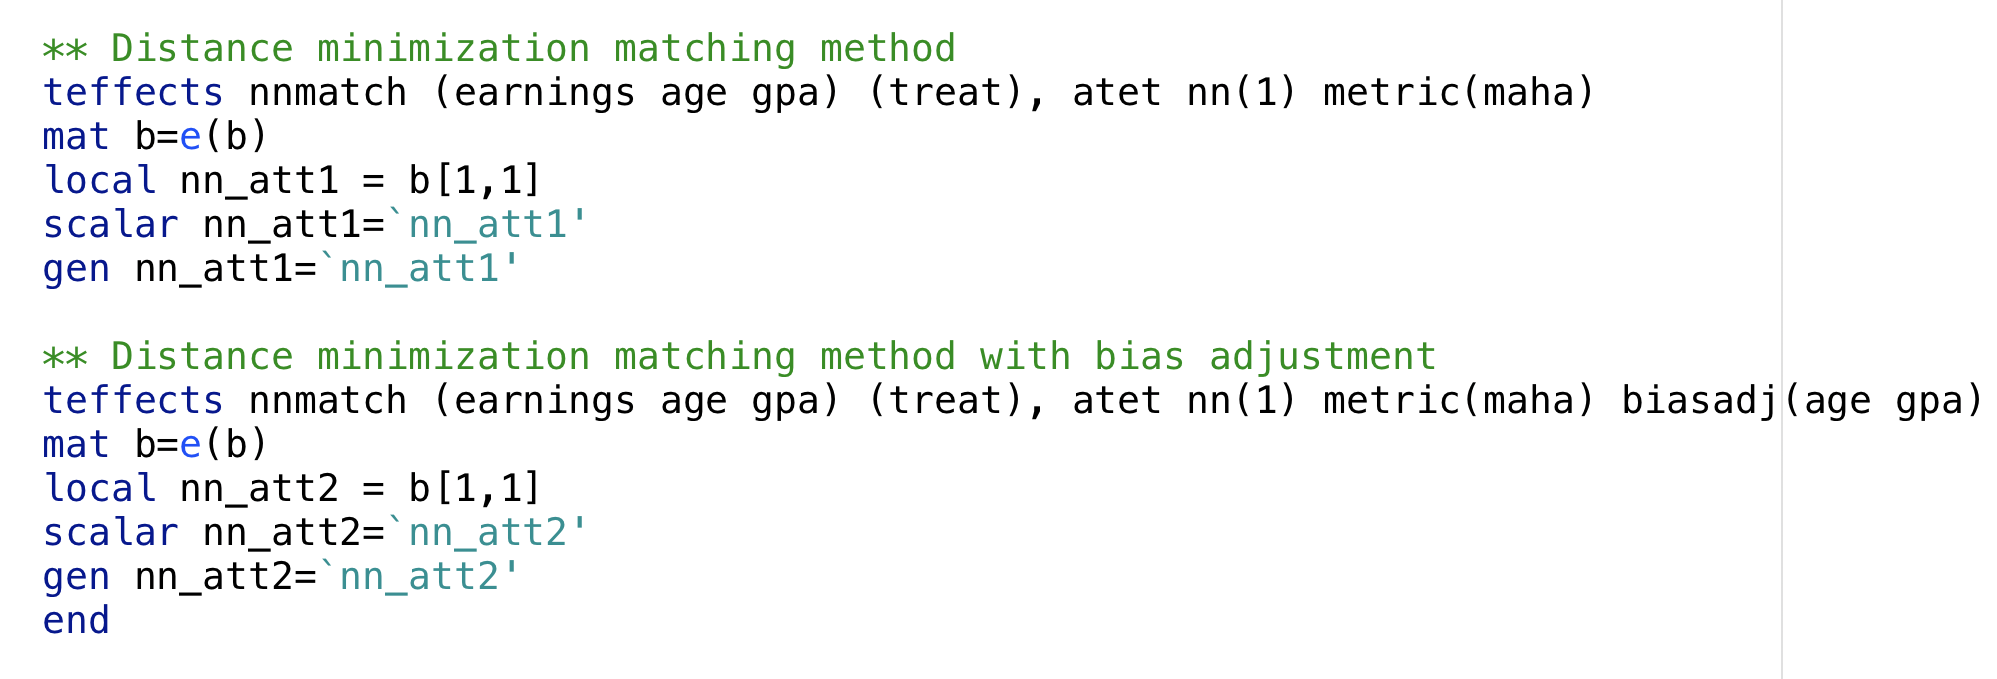
\includegraphics[scale=0.325]{./lecture_includes/nonlinear_matching}
\end{figure}

\end{frame}

\begin{frame}{Nonlinear DGP, OLS and Matching}

\begin{figure}[!t]\centering
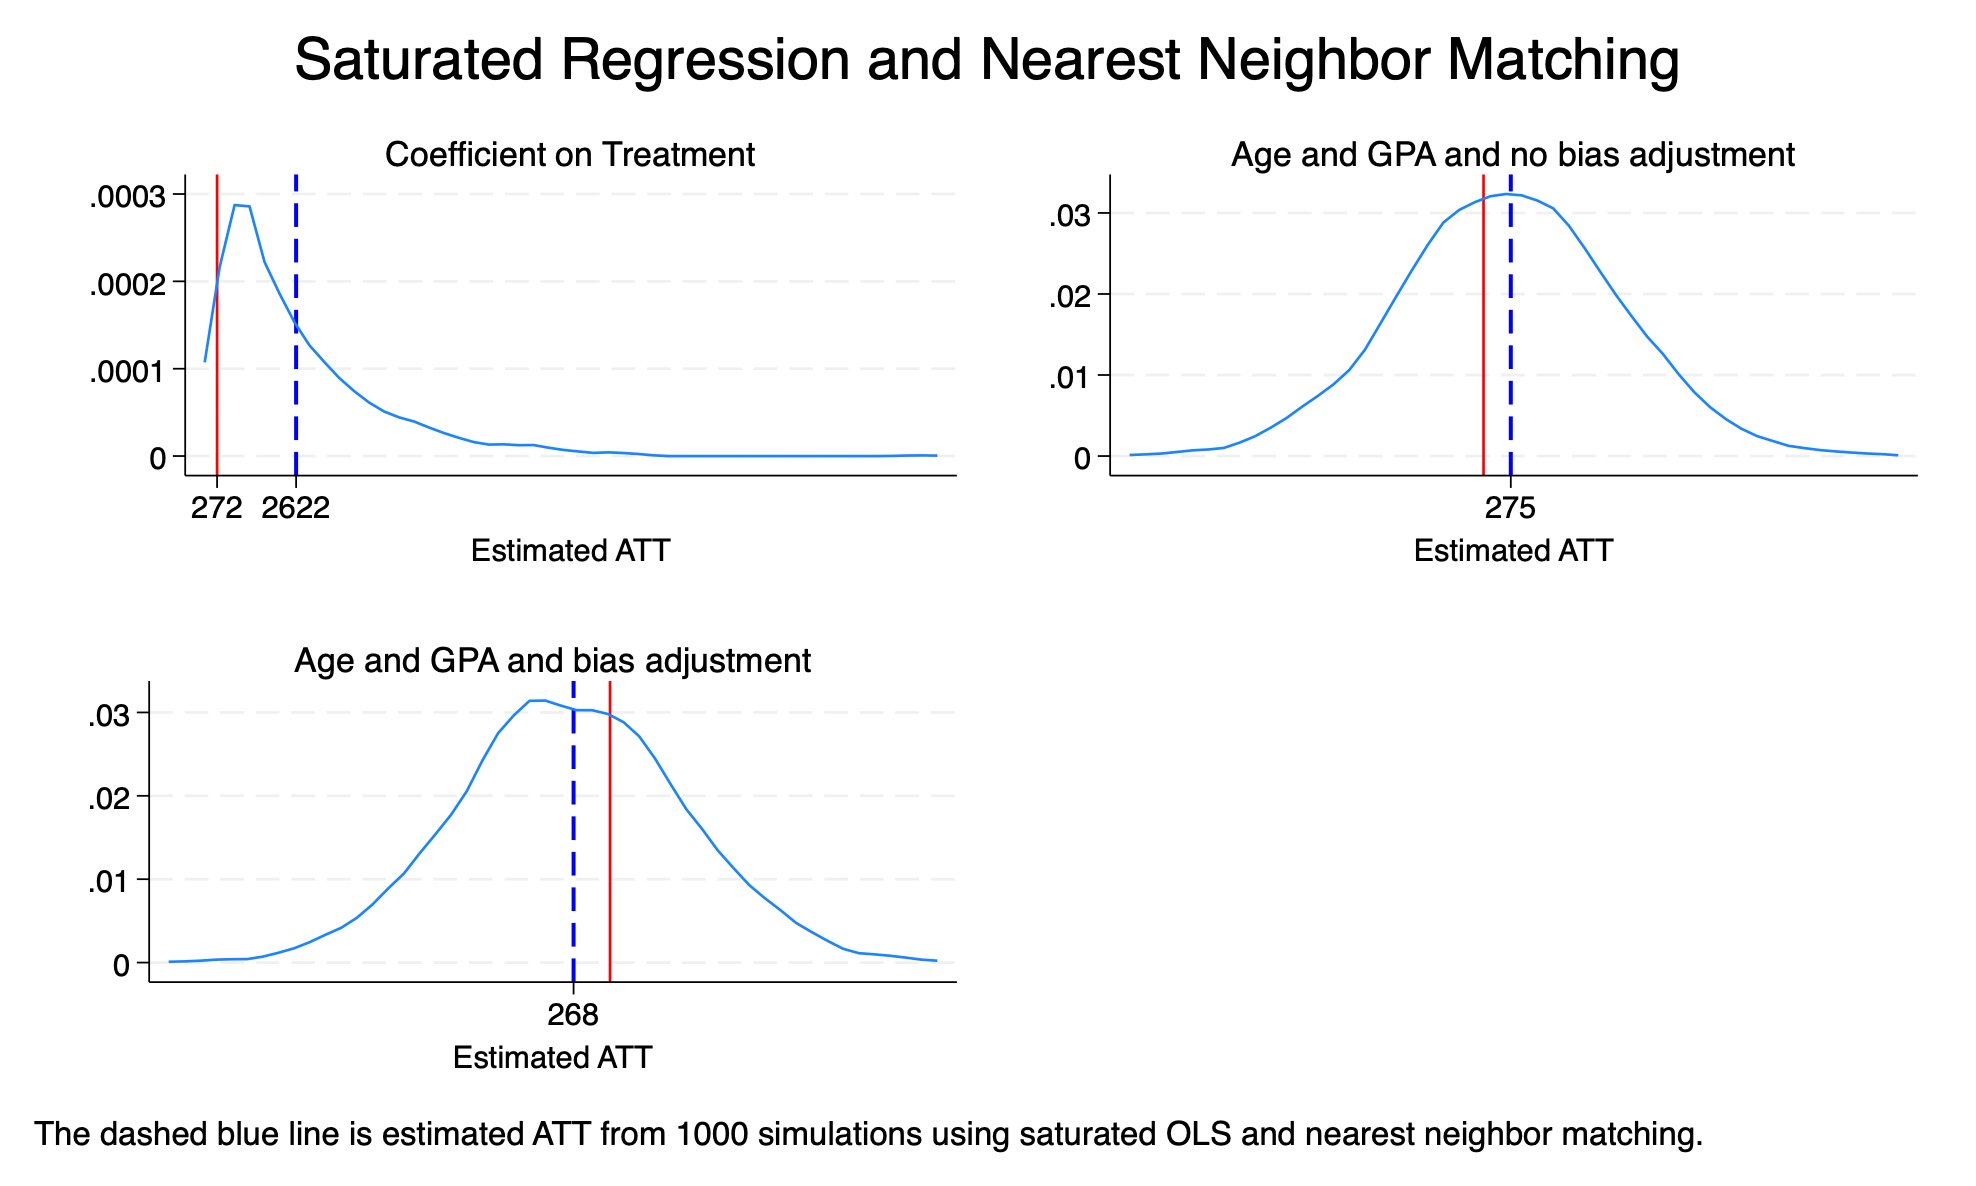
\includegraphics[scale=0.175]{./lecture_includes/nonlinear_att.jpg}
\end{figure}

\end{frame}





\subsection{What is your coefficient an average of?}

\begin{frame}{Back up. What \emph{is} that coefficient?}

You ran this and read $\widehat{\delta}$ off the output:

$$Y_i = \alpha + \delta D_i + \beta X_i + \varepsilon_i$$

\begin{itemize}
\item With heterogeneous effects, $\widehat{\delta}$ is an average of \emph{something}
\item The question is what, and with what weights
\item Two papers answer it. Twenty-four years apart
\end{itemize}

\end{frame}


\begin{frame}{Angrist (1998): the variance weights}

\textbf{Binary $D$, discrete controls $G$.} Apply FWL and the algebra falls out:

$$\beta_1 = \sum_g w_g \, \tau_g, \qquad
  w_g = \frac{\Pr(G=g)\, p_g(1-p_g)}{\sum_{g'}\Pr(G=g')\, p_{g'}(1-p_{g'})}$$

\begin{itemize}
\item $\tau_g$ is the within-stratum effect --- each one correctly estimated
\item But the weights are \emph{not} the population shares $\Pr(G=g)$
\item They're population share $\times$ \highlight{treatment variance} $p_g(1-p_g)$
\end{itemize}

\end{frame}


\begin{frame}{Why $p_g(1-p_g)$? Because OLS likes a coin flip}

\centering
\begin{tikzpicture}[scale=0.95]
  \node[draw=ocean, fill=ocean!8, rounded corners=3pt, minimum width=2.9cm,
        minimum height=1.2cm, align=center, font=\small] (size) at (-3.1,0)
    {\textbf{Stratum size}\\[2pt] $\Pr(G=g)$};
  \node[font=\large, text=charcoal] at (-1.2,0) {$\times$};
  \node[draw=forest, fill=forest!8, rounded corners=3pt, minimum width=3.1cm,
        minimum height=1.2cm, align=center, font=\small] (var) at (0.8,0)
    {\textbf{Treatment variance}\\[2pt] $p_g(1-p_g)$};
  \node[font=\large, text=charcoal] at (2.75,0) {$\propto$};
  \node[draw=harvardcrimson, fill=harvardcrimson!8, rounded corners=3pt,
        minimum width=1.9cm, minimum height=1.2cm, align=center, font=\small] at (4.4,0)
    {\textbf{Weight}\\[2pt] $w_g$};
\end{tikzpicture}

\vspace{1em}
\raggedright

\begin{itemize}
\item $p_g(1-p_g)$ peaks at $p_g = 0.5$ and vanishes at 0 or 1
\item Strata where treatment looks like a coin flip get \emph{more} weight
\item Strata where almost everyone is treated (or nobody) get almost none
\item Makes sense as \emph{precision}. Makes no sense as a \emph{population}
\end{itemize}

\end{frame}


\begin{frame}{A job training program run at two sites}

\begin{itemize}
\item \textbf{Site A} had plenty of slots. They randomized with a \emph{coin flip}
\item \textbf{Site B} was budget-rationed. You got a slot only if you \emph{rolled a six}
\end{itemize}

\vspace{0.7em}

\centering
{\small
\begin{tabular}{lcccr}
\toprule
Site & $N$ & $p_g$ & Treated / Control & $\tau_g$ \\
\midrule
A & 300 & $1/2$ & 150 / 150 & $-\$9{,}000$ \\
B & 600 & $1/6$ & 100 / 500 & $+\$6{,}000$ \\
\bottomrule
\end{tabular}}

\vspace{0.8em}
\raggedright

\begin{itemize}
\item Site A pulled people out of jobs they already had --- lock-in, and it cost them
\item Site B genuinely helped
\item $ATE = \tfrac{1}{3}(-9{,}000) + \tfrac{2}{3}(6{,}000) = \highlight{+\$1{,}000}$
\end{itemize}

\end{frame}


\begin{frame}{Now run the regression}

\centering
{\small
\begin{tabular}{lccccr}
\toprule
Site & $\Pr(G)$ & $p_g(1-p_g)$ & $w_g$ & $\tau_g$ & \\
\midrule
A & $1/3$ & 0.250 & \textbf{0.474} & $-\$9{,}000$ & \\
B & $2/3$ & 0.139 & \textbf{0.526} & $+\$6{,}000$ & \\
\bottomrule
\end{tabular}}

\vspace{0.8em}

$$\beta_{OLS} = 0.474(-9{,}000) + 0.526(6{,}000) = \highlight{-\$1{,}105}$$

\vspace{0.6em}
\raggedright

\begin{itemize}
\item Site A is a third of the population and gets \emph{half} the weight
\item Because a coin flip has more treatment variance than a die
\item \alert{The program raises earnings by \$1,000. OLS says it lowers them by \$1,100}
\end{itemize}

\end{frame}


\begin{frame}{The gap needs \emph{both} kinds of variation}

\begin{itemize}
\item $\tau_g$ constant $\Rightarrow$ $\beta = \sum_g w_g \tau = \tau = ATE$. No gap
\item $p_g$ constant $\Rightarrow$ $w_g = \Pr(G=g)$. No gap
\end{itemize}

\vspace{0.8em}

\begin{itemize}
\item You need heterogeneous effects \emph{and} uneven take-up
\item An RCT with $p_g = 0.5$ everywhere: no gap
\item Observational data with selection: gap essentially always
\item Same structure as our balance slide --- imbalance has to interact with something
\end{itemize}

\end{frame}


\subsection{Sloczynski and the reversal}

\begin{frame}{Sloczynski (2022): say it in ATT and ATU}

Angrist decomposes into \emph{strata}. Tymon decomposes into the two parameters we name:

$$\tau = \omega_1 \cdot ATT + \omega_0 \cdot ATU$$

\vspace{0.5em}

\begin{itemize}
\item Same coefficient. Different bookkeeping
\item Our two sites: $ATT = -\$3{,}000$, $ATU = +\$2{,}538$, $\omega_1 = 0.658$
\item $0.658(-3{,}000) + 0.342(2{,}538) = \highlight{-\$1{,}105}$ --- the same number as Angrist
\end{itemize}

\end{frame}


\begin{frame}{And now look at the weights}

\centering
\begin{tikzpicture}[scale=1.0]
  \draw[warmgray] (0.2,0) -- (6.4,0);

  \fill[forest!65]        (0.8,0) rectangle (1.7,1.389);
  \node[font=\small, anchor=south] at (1.25,1.41) {0.28};
  \node[font=\scriptsize, anchor=north, align=center] at (1.25,-0.15)
    {what the ATE\\needs ($\rho$)};

  \fill[harvardcrimson!70] (4.0,0) rectangle (4.9,3.289);
  \node[font=\small, anchor=south] at (4.45,3.31) {0.66};
  \node[font=\scriptsize, anchor=north, align=center] at (4.45,-0.15)
    {what OLS\\gives ($\omega_1$)};

  \node[font=\scriptsize, text=warmgray, anchor=south] at (3.1,3.75) {weight on the ATT};
\end{tikzpicture}

\vspace{1.6em}
\raggedright

\begin{itemize}
\item $ATE = \rho \cdot ATT + (1-\rho)\cdot ATU$ with $\rho = 0.28$
\item OLS uses $\omega_1 = 0.66 \approx 1 - \rho$
\item \highlight{The weights are flipped} --- and here that flips the sign too
\end{itemize}

\end{frame}


\begin{frame}{So why did we need Tymon if we had Angrist?}

\centering
{\small
\begin{tabular}{lll}
\toprule
 & \textbf{Angrist (1998)} & \textbf{Sloczynski (2022)} \\
\midrule
Controls        & discrete, saturated      & any $X$ \\
Decomposes into & stratum effects $\tau_g$ & $ATT$ and $ATU$ \\
Weights         & $\Pr(g)p_g(1-p_g)$       & $\omega_1 \approx 1-\rho$ \\
Need to know    & the whole joint dist.    & the treated share \\
Misspecified?   & no --- it's saturated     & yes, generally \\
\bottomrule
\end{tabular}}

\vspace{0.9em}
\raggedright

\begin{itemize}
\item They agreed on our example \emph{because} two sites \emph{is} a saturated model
\item That's the special case where the two coincide
\item \highlight{Angrist says it's a weighted average. Tymon says the weights are backwards}
\end{itemize}

\end{frame}




\begin{frame}{You'll see this exact move again next week}

\begin{itemize}
\item Goodman-Bacon (2021): twoway fixed effects with staggered adoption
\item Same result, different setting --- the estimate is a weighted average of every
      possible $2\times 2$ DiD
\item Weights again $\propto$ group size $\times$ treatment variance
\item And again the pathology is the weights, not the comparisons
\end{itemize}

\vspace{0.6em}

\deemph{Once you've seen it here, Bacon's decomposition is the same story wearing a panel-data coat.}

\end{frame}












\begin{frame}{Two diagnostics you can run before lunch}

Both need only $\rho$, the treated share:

\begin{itemize}
\item Going for the \textbf{ATT}? The damage is $\rho$
\item Going for the \textbf{ATE}? The damage is $|2\rho - 1|$ --- twice your distance from 50/50
\end{itemize}

\vspace{0.7em}

\begin{itemize}
\item Each is the fraction of the $ATU - ATT$ gap that leaks into your estimate
\item So OLS is fine for the ATE when the arms are similar in size
\item And fine for the ATT only when very few are treated
\item \texttt{hettreatreg} in R and Stata reports these for you
\end{itemize}

\end{frame}


\begin{frame}{Where the gap comes from}

Sloczynski splits the distance between your coefficient and your target in two:

$$\beta_{OLS} - ATE \;=\; \underbrace{\text{bias from nonlinearity}}_{\text{wrong functional form}}
  \;+\; \underbrace{\text{bias from heterogeneity}}_{\text{wrong weights}}$$

\vspace{0.6em}

\begin{itemize}
\item Saturate the model and the first term goes away
\item The second one does \emph{not} --- that's the reversal, and no amount of flexibility fixes it
\item You fix it by changing the \emph{estimator}, not the specification
\end{itemize}

\end{frame}

































\begin{frame}{Stata exercises}

We will now look at two simulations to help you understand both of these

\end{frame}















\begin{frame}{Visualizing the problem one way}
    \begin{figure}
        \centering
        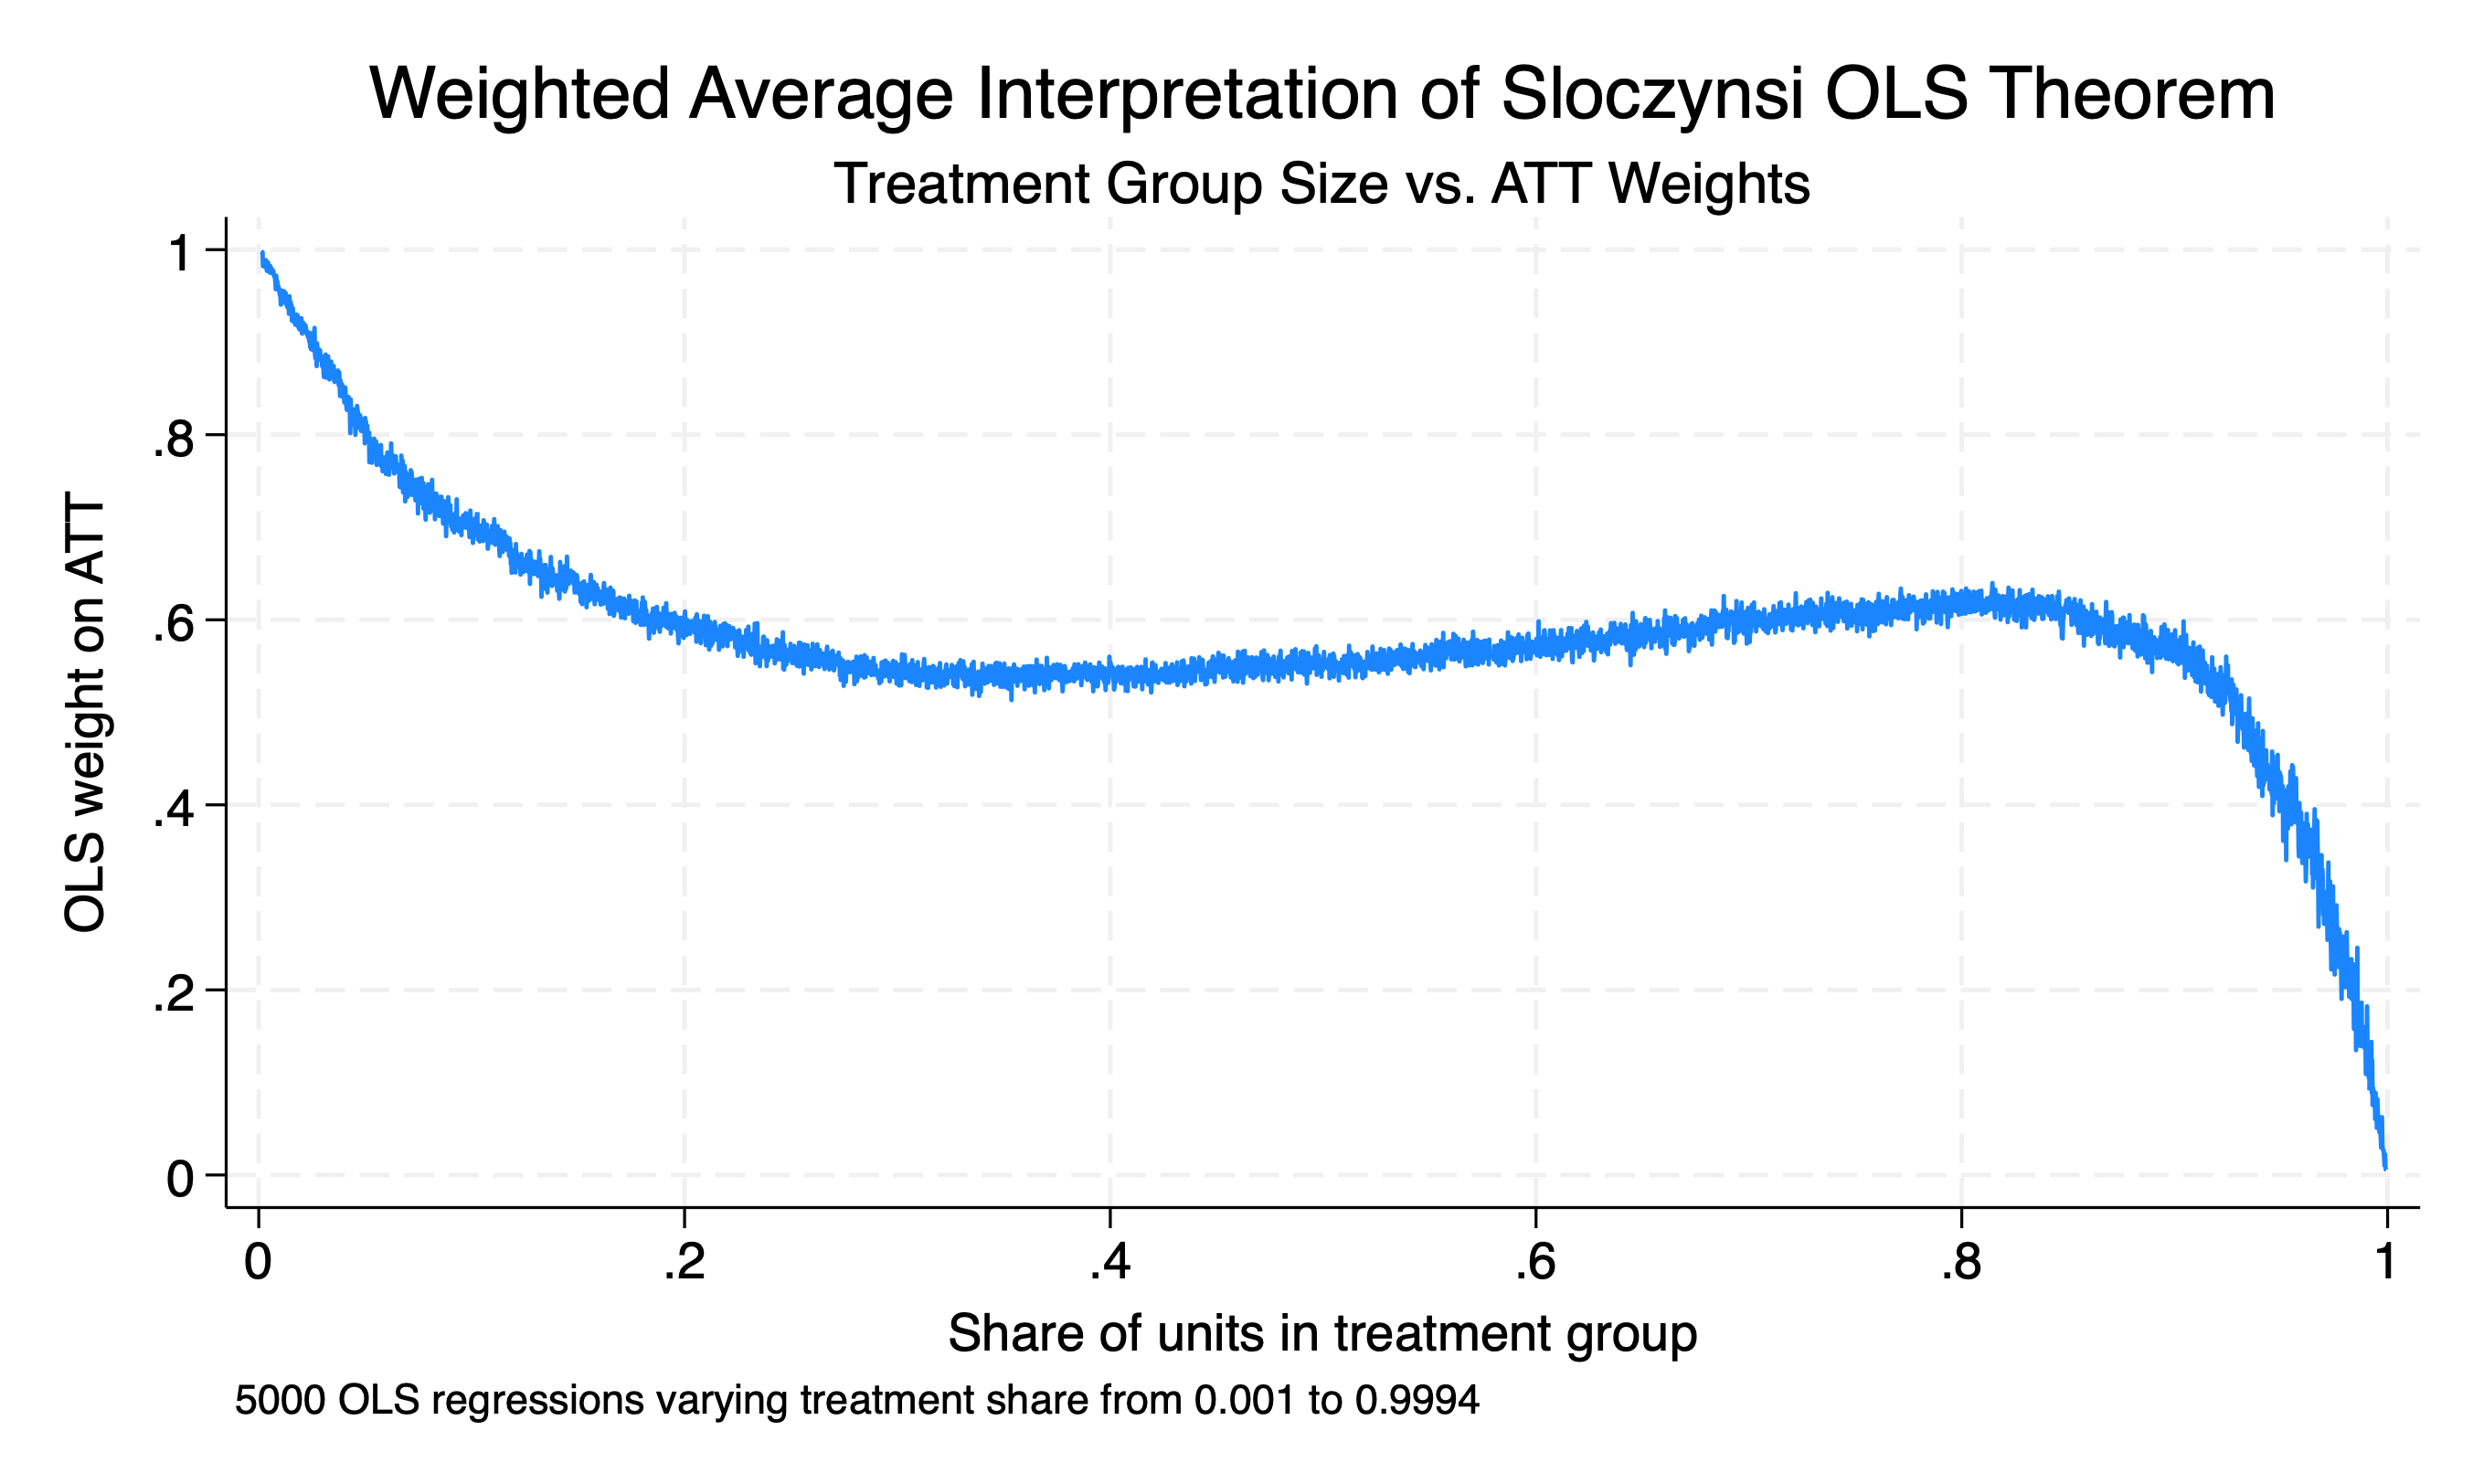
\includegraphics[width=0.8\textwidth]{./lecture_includes/tymon_weights_crossing}
        \caption{As more units are placed in treatment, the weight OLS puts on the ATT \emph{falls}.}
    \end{figure}
\end{frame}

\begin{frame}{The coefficient sweeps with the treated share}
    \begin{figure}
        \centering
        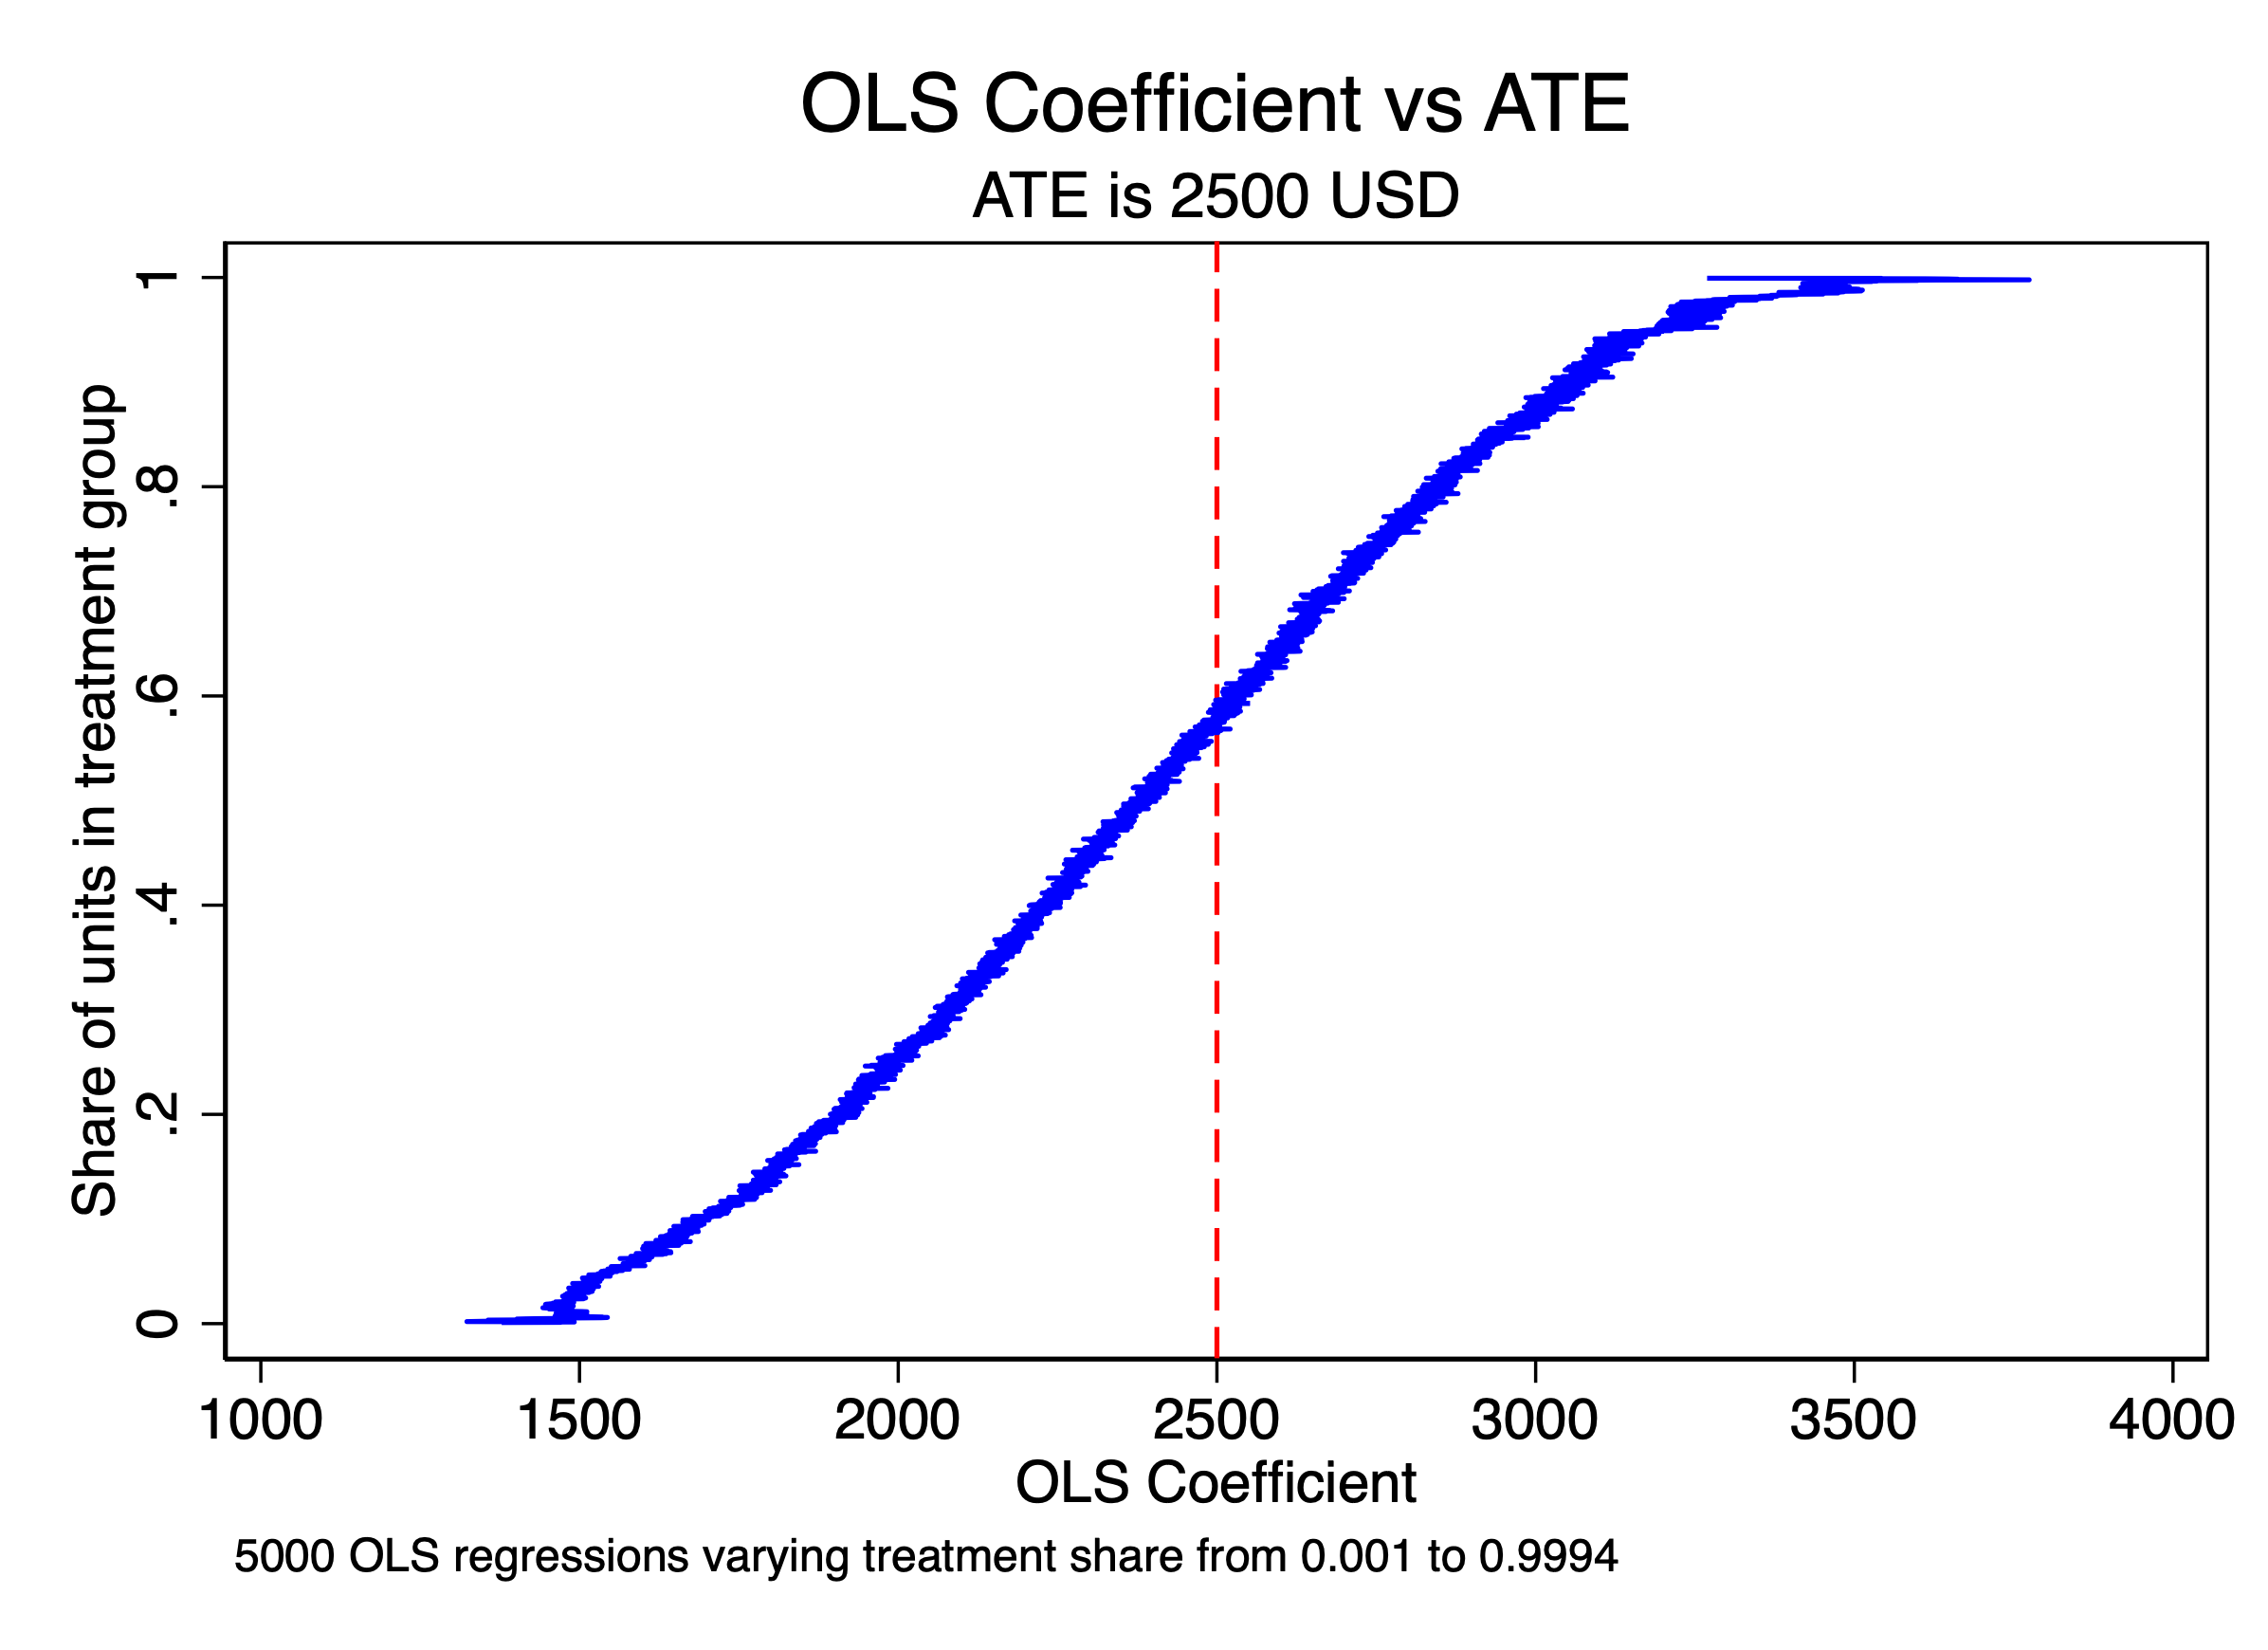
\includegraphics[width=0.74\textwidth]{./lecture_includes/ols_ate.png}
        \caption{Few treated (bottom left): OLS leans toward the ATT (\$1,962). Many treated (top right): toward the ATU (\$3,037). It hits the true ATE of \$2,500 only in between.}
    \end{figure}
\end{frame}











\begin{frame}
\frametitle{Prevalence of OLS Bias in Evaluating Labor Market Programs}
\begin{itemize}
  \item OLS may frequently show substantial bias for ATE and ATT in published studies
  \item In studies like Card, Kluve, and Weber (2018), with a mean treatment rate of 17.7\%, biases are common:
    \begin{itemize}
      \item The expected bias in OLS for ATE is 64.6\% of the ATU-ATT difference.
      \item For ATT, the expected OLS bias is 17.7\% of the ATU-ATT difference.
    \end{itemize}
  \item These findings indicate that biases in OLS estimates could often be significant.
    \begin{itemize}
      \item LaLonde's (1986) training program effects aligning with ATT.
      \item Aizer et al.'s (2016) cash transfer effects resembling ATU.
    \end{itemize}
  \item Implementation of results is available in R and Stata through the \texttt{hettreatreg} packages.
\end{itemize}
\end{frame}




\begin{frame}{Tymon's replication of Angrist and Pischke}
    \begin{figure}
        \centering
        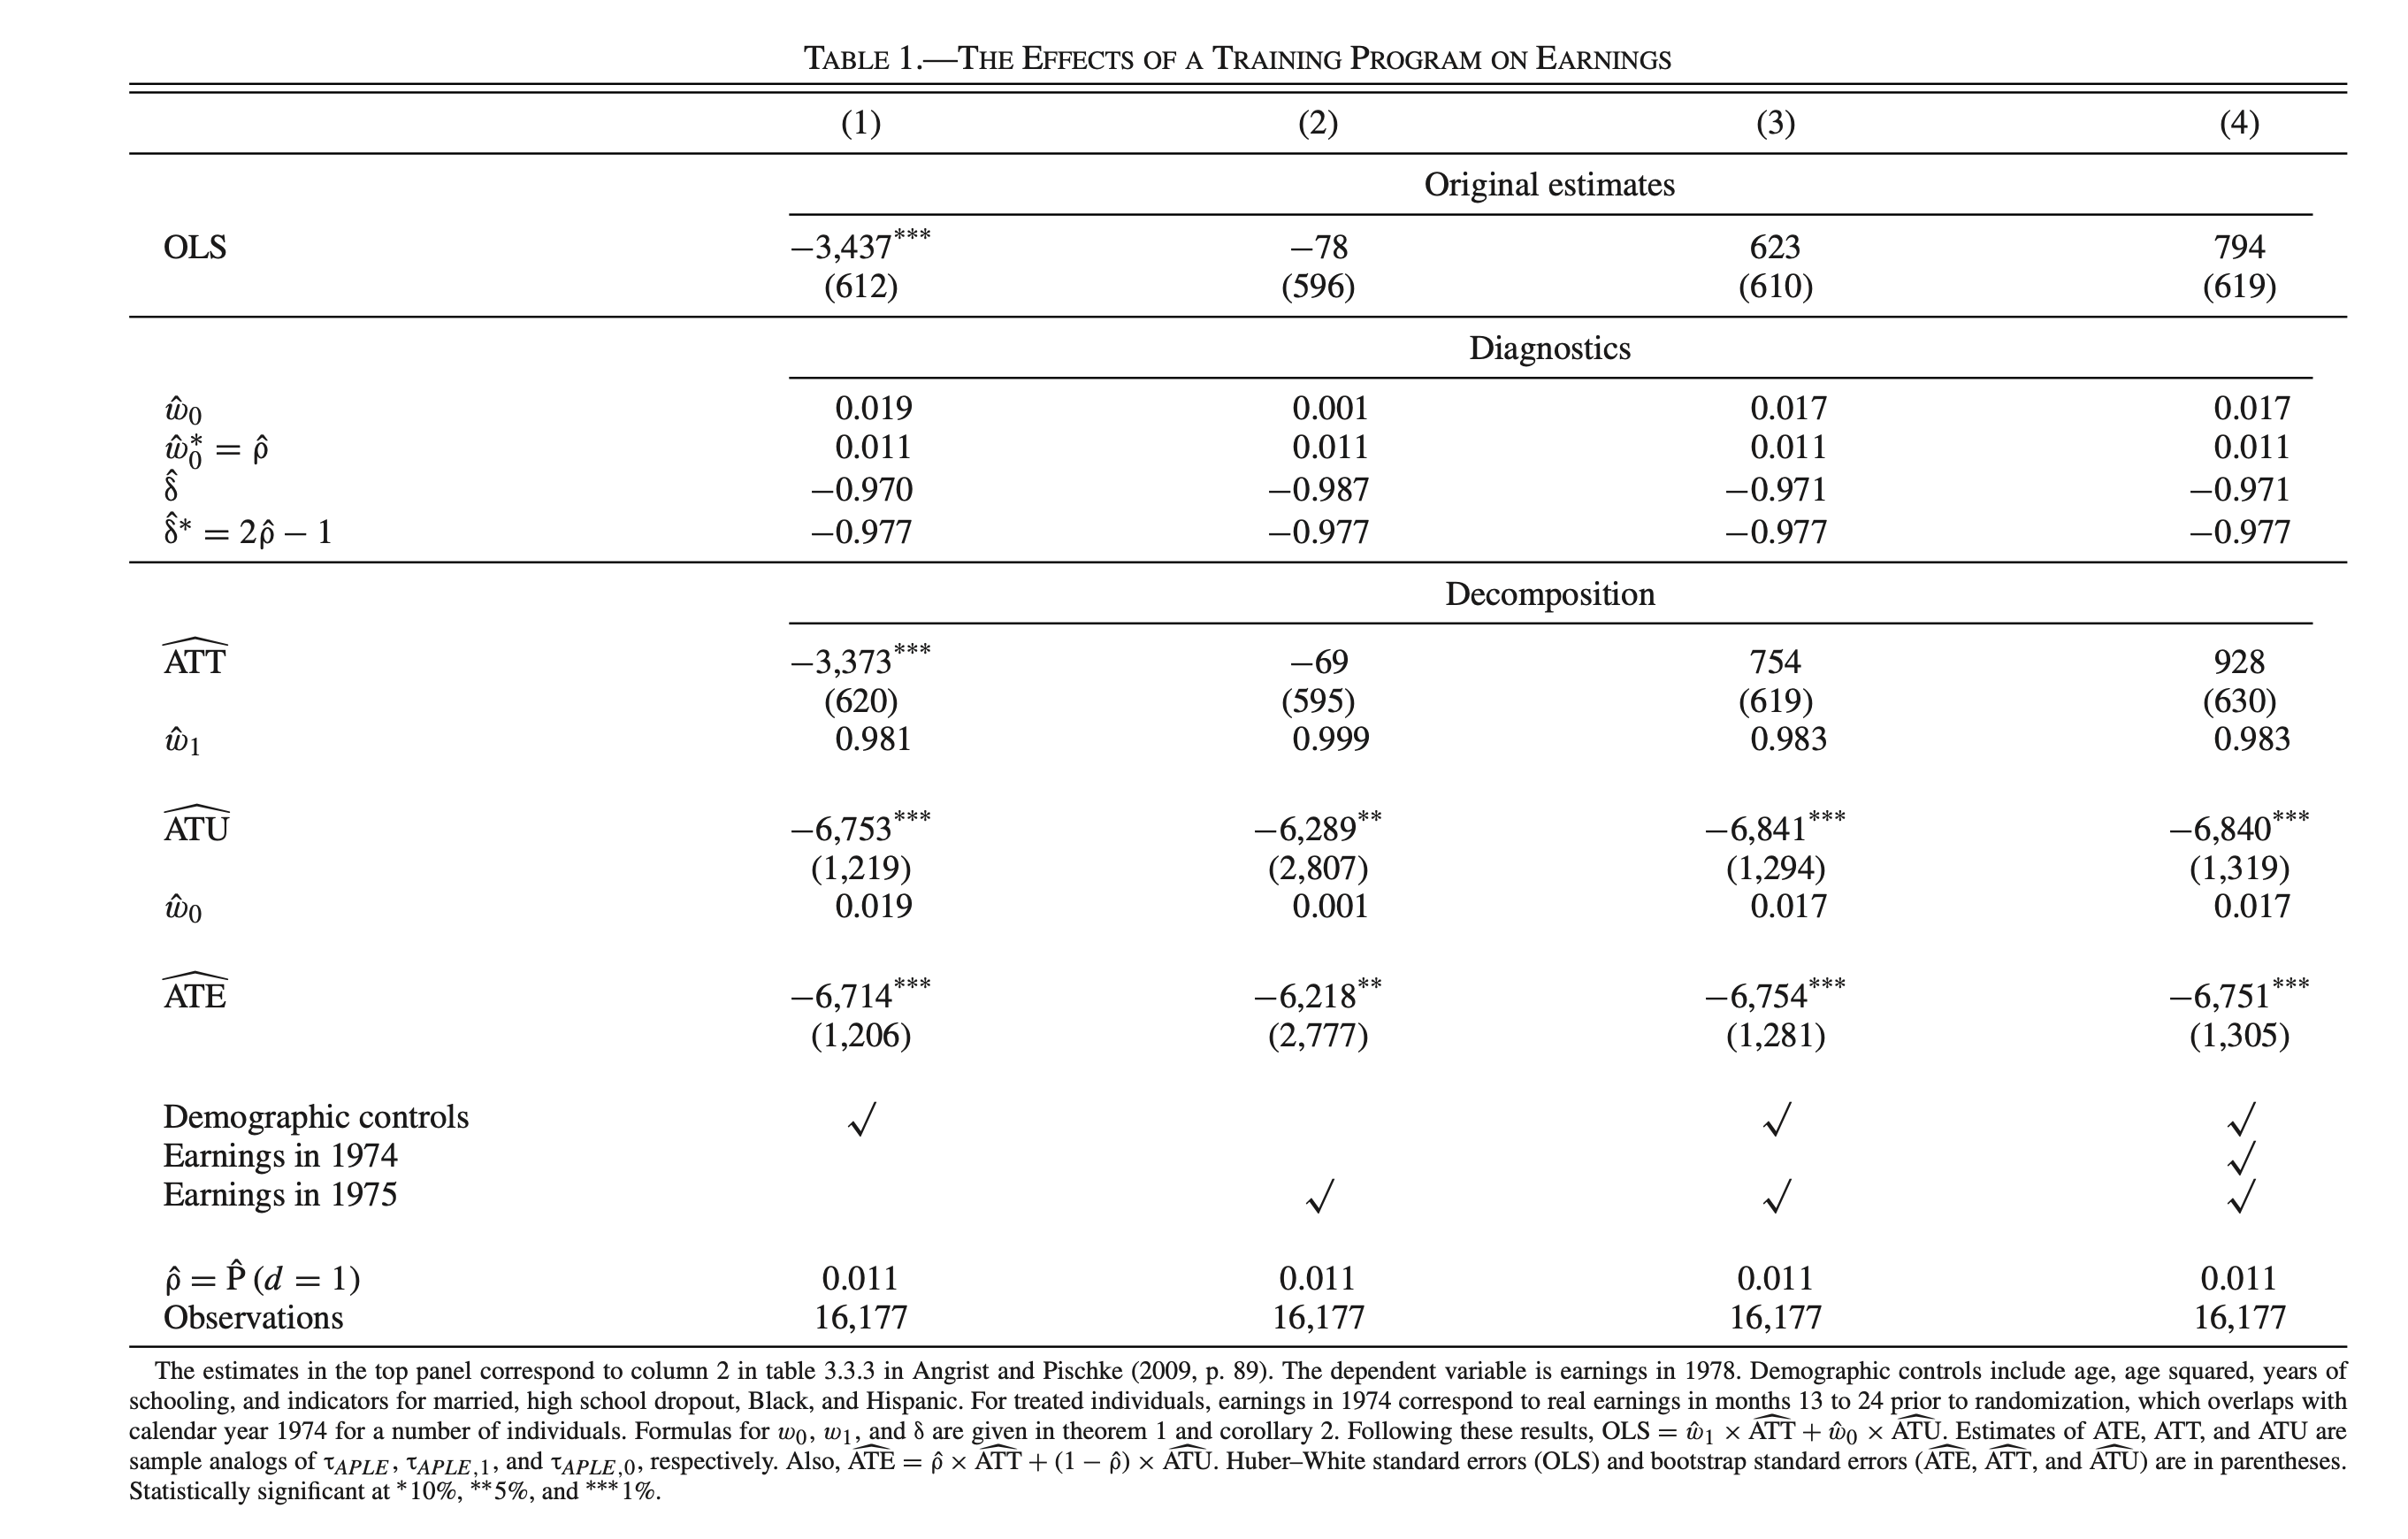
\includegraphics[width=0.8\textwidth]{./lecture_includes/tymon_lalonde_table1.png}
    \end{figure}
\end{frame}

\begin{frame}{Stata simulation}

Let's do this ourselves using lalonde.do in the labs/matching on github repo

\end{frame}


\begin{frame}
\frametitle{Replications of Lalonde data using Dehejia and Wahba sample with CPS control}

\tiny
\begin{tabular}{lccccc}
\hline \hline
 & \multicolumn{5}{c}{Dependent variable: Real earnings in 1978} \\
 & (1) & (2) & (3) & (4) & (5) \\
Controls: & No controls & Demographics & RE75 Only & Demo and RE75 & Demo, RE74 and RE75 \\
\hline
Treatment                 &   -8497.516***&   -3436.795***&     -77.705   &     622.547   &     \textbf{793.587}   \\
                    		&   (581.916)   &   (612.056)   &   (596.215)   &   (609.582)   &   (618.609)   \\
\hline \end{tabular}

\bigskip

Each column corresponds to a set of observable controls below:
\begin{itemize}
\item Demographics: Age, Age-squared, Years of schooling, Marriage dummy, High school dropout dummy, Black and Hispanic dummies
\item Real earnings in 1975 (RE75)
\item Real earnings in 1974 (RE74)
\end{itemize}

Our focus will be on the last estimate.  Question is what is this?

\end{frame}



\begin{frame}{What that \$794 actually was}

Interact treatment with every covariate and all three parameters fall out:

\vspace{0.5em}

\centering
{\small
\begin{tabular}{lr}
\toprule
$\widehat{ATE}$ & $-\$4{,}930$ \\
$\widehat{ATT}$ & $+\$796$ \\
$\widehat{ATU}$ & $-\$4{,}996$ \\
\midrule
OLS coefficient & $+\$794$ \\
\bottomrule
\end{tabular}}

\vspace{0.7em}
\raggedright

\begin{itemize}
\item Only 1.1\% of the sample is treated --- so OLS put \highlight{99.96\%} of its weight on the ATT
\item Which is why it looked ``close to the experimental benchmark''
\item \alert{The OLS estimate and the ATE have opposite signs}
\end{itemize}

\end{frame}


\subsection{So what do you actually run?}

\begin{frame}{Diagnosis is not a method}

\begin{itemize}
\item Everything so far tells you what goes wrong. None of it tells you what to run
\item But the fix has been sitting in that last table the whole time
\item We got the ATE, the ATT \emph{and} the ATU out of one regression
\item By interacting the treatment with every covariate
\end{itemize}

\vspace{0.7em}

\deemph{That estimator has a name, and it is older than the problem it solves.}

\end{frame}


\begin{frame}{Regression adjustment}

Fit the two potential-outcome surfaces \emph{separately}:

$$\widehat{\mu}^1(X) \ \text{on the treated}, \qquad \widehat{\mu}^0(X) \ \text{on the controls}$$

Then impute everyone's missing side and average over whichever population your estimand names:

\begin{itemize}
\item Average over \emph{everyone} $\to$ ATE
\item Average over the \emph{treated} $\to$ ATT
\item Average over the \emph{untreated} $\to$ ATU
\end{itemize}

\vspace{0.5em}

\highlight{You choose the weights. OLS chose them for you.}

\end{frame}


\begin{frame}{This is Oaxaca-Blinder}

\begin{itemize}
\item Oaxaca (1973) and Blinder (1973) built it to decompose the black-white and
      male-female wage gap
\item Separate wage equations by group, then ask how much of the gap is
      composition and how much is returns
\item Structurally identical to what we just did
\item Kline (2011) showed the ``unexplained component'' \emph{is} a treatment effect
      estimator --- and a doubly robust one
\item Also called regression adjustment (Wooldridge 2010; Graham and Pinto 2022)
\end{itemize}

\end{frame}


\begin{frame}{A footnote you'll enjoy}

\begin{itemize}
\item Ron Oaxaca was Orley Ashenfelter's student in the Princeton Industrial Relations Section
\item The same room we started the day in
\item The tool built there in 1973 to measure discrimination turns out to be
      the repair for a problem economists wouldn't name until 2022
\end{itemize}

\vspace{0.6em}

\deemph{Two rivers, one estimator.}

\end{frame}


\begin{frame}{In practice}

\begin{itemize}
\item Stata: \texttt{teffects ra (y X) (d)} --- and \texttt{atet} if you want the ATT
\item R: \texttt{estimatr::lm\_lin}, or the \texttt{hettreatreg} package for the diagnostics
\item Do it by hand once so you believe it, then let the software do it
\item Full interaction is easy to botch --- we saw the ``comically long'' version earlier
\end{itemize}

\vspace{0.6em}

\begin{itemize}
\item \texttt{comparing.do} in \texttt{/Lab/Matching} runs all of it side by side
\item Additive OLS, matching, bias-corrected matching, and regression adjustment
\item Against a known $ATE = \$2{,}500$, $ATT = \$1{,}962$, $ATU = \$3{,}037$
\end{itemize}

\end{frame}


\begin{frame}{But regression adjustment is not free either}

\begin{itemize}
\item It still fits $\widehat{\mu}^0(X)$ where the treated live --- often where no controls are
\item That is extrapolation, and it comes from the functional form, not the data
\item Matching refuses to do this. It just tells you it has no match
\item Neither is safer. One hides the assumption, the other reports it
\end{itemize}

\vspace{0.6em}

\deemph{Losing common support is not a problem you escape by switching to a regression.}

\end{frame}


\begin{frame}{OLS doesn't stop at the edge of the data}

\centering
\begin{tikzpicture}[scale=0.70]
  \draw[-stealth, warmgray] (0,0) -- (9.2,0) node[anchor=north east, font=\scriptsize] {$X$};
  \draw[-stealth, warmgray] (0,0) -- (0,6.4) node[anchor=south west, font=\scriptsize] {$Y$};

  \draw[warmgray, dashed, thin] (3.6,0) -- (3.6,6.0);
  \draw[warmgray, dashed, thin] (4.2,0) -- (4.2,6.0);
  \node[font=\scriptsize, text=charcoal, anchor=south] at (3.9,6.05) {common support};

  \fill[ocean] (1.6,4.1) circle (2.2pt);
  \fill[ocean] (2.2,3.9) circle (2.2pt);
  \fill[ocean] (2.8,4.4) circle (2.2pt);
  \fill[ocean] (3.4,4.2) circle (2.2pt);
  \fill[ocean] (4.0,4.8) circle (2.2pt);

  \draw[warmgray] (3.8,3.0) circle (2.2pt);
  \draw[warmgray] (4.6,3.9) circle (2.2pt);
  \draw[warmgray] (5.4,3.7) circle (2.2pt);
  \draw[warmgray] (6.2,4.8) circle (2.2pt);
  \draw[warmgray] (7.0,4.6) circle (2.2pt);
  \draw[warmgray] (7.8,5.5) circle (2.2pt);

  \draw[ocean, line width=1.3pt] (1.6,3.88) -- (4.0,4.60);
  \draw[warmgray, line width=1.3pt] (3.8,3.29) -- (7.8,5.49);
  \draw[harvardcrimson, line width=1.2pt, dashed] (3.8,3.29) -- (0,1.20);

  \draw[stealth-stealth, harvardcrimson, line width=1pt] (2.2,2.41) -- (2.2,4.06);
  \fill[harvardcrimson] (2.2,2.41) circle (2.4pt);
  \fill[harvardcrimson] (0,1.20) circle (2.8pt);
  \node[font=\scriptsize, text=harvardcrimson, anchor=west] at (0.2,0.65) {$\widehat{\alpha}$: nobody is here};
  \node[font=\scriptsize, text=harvardcrimson, anchor=west] at (2.45,2.3) {invented};

  \fill[ocean] (5.5,0.9) circle (2.2pt);
  \node[font=\scriptsize, anchor=west] at (5.75,0.9) {treated};
  \draw[warmgray] (7.4,0.9) circle (2.2pt);
  \node[font=\scriptsize, anchor=west] at (7.65,0.9) {controls};
\end{tikzpicture}

\vspace{0.8em}
\raggedright

\begin{itemize}
\item Solid where the group has data. Dashed is invented
\item No control unit sits at $X=2.2$ --- that counterfactual is pure \highlight{slope}
\item And $\widehat{\alpha}$ describes a person who isn't in the data
\end{itemize}

\end{frame}


\begin{frame}{Why this happens: the curse of dimensionality}

\begin{itemize}
\item One covariate and the gap is visible. You just saw it
\item Add a second and you need overlap in the \emph{rectangle}, not the margins
\item $k$ covariates, three bins each, and you have $3^k$ cells to fill
\end{itemize}

\vspace{0.7em}

\begin{itemize}
\item Cells empty out long before you notice
\item The propensity score \emph{summarizes} those cells --- it does not populate them
\item So a balanced-looking weight can sit on top of cells with nobody in them
\end{itemize}

\end{frame}


\begin{frame}{Two honest ways to lose}

\centering
{\small
\begin{tabular}{lll}
\toprule
 & \textbf{Matching / weighting} & \textbf{OLS / regression adjustment} \\
\midrule
No match?      & refuses, drops the unit  & extrapolates from the slope \\
What you get   & a smaller sample         & a full-sample number \\
The assumption & visible                  & buried in functional form \\
Fails by       & losing your estimand     & quietly being wrong \\
\bottomrule
\end{tabular}}

\vspace{1.1em}
\raggedright

\begin{itemize}
\item Both can be right. Both can be wrong
\item \highlight{Neither one gives you back the data you don't have}
\item So go look at the cells before you pick
\end{itemize}

\end{frame}


\begin{frame}{Concluding remarks}

\begin{itemize}

\item Last years have shown a \emph{particular} OLS specification yields biased estimates of all causal parameters when there exists heterogeneity in the treatment effects
	\begin{itemize}
	\item Goodman-Bacon (2021) for instance showed this with the common twoway fixed effects specification and dynamic treatment effects
	\end{itemize}
\item Turns out it was not a diff-in-diff problem only -- it's an OLS problem more generally
	\begin{itemize}
	\item We saw it also in a paper by Goldsmith-Pinkham, Hull and Kolsar on contamination bias in linear models with multiple treatment effects and heterogeneity
	\end{itemize}
\item Here we see the perversity of the effects under unconfoundedness and heterogeneity which is the OLS coefficient counterinuititvely favors the smaller groups and therefore their causal parameters
\end{itemize}

\end{frame}

\begin{frame}{Concluding remarks}

\begin{itemize}

\item We mentioned work by Anna Aizer more likely is estimating coefficients that are more like the ATU than either the ATE or the  ATT because of how large the treatment group is
\item This has implications for analysis in which the proportion of groups differ in size due to population differences or over-representation of one group over another (i.e., Asians in criminal justice)
\item The smaller the group, the larger their influence on the OLS coefficient
\item Lesson here is that regression adjustment as well as nearest neighbor matching with bias adjustment may need to be your core models, not the additive in covariates OLS specification we are accustomed to

\end{itemize}

\end{frame}




\section{Advice}


\begin{frame}{Design before analysis}

\begin{itemize}
\item Almost all of the work happens \emph{before} you touch the outcome
\item Who chose the treatment? What did they know? Why did they do it?
\item If you can't answer that, you're not ready to estimate anything
\item The estimator is the last decision you make, not the first
\end{itemize}

\vspace{0.6em}

\deemph{Imbens and Xu (2024) put this first on their list too.}

\end{frame}


\begin{frame}{If you claim unconfoundedness, you owe us two pictures}

\begin{itemize}
\item A \highlight{propensity score plot} by arm --- so we can see the overlap
\item A \highlight{balance table} with normalized differences --- so we can see the imbalance
\end{itemize}

\vspace{0.8em}

\begin{itemize}
\item Normalized differences, not $t$-stats
\item Both are cheap. Both are observable. Their absence is a choice
\item You must adjust for the confounders \emph{insofar as they are imbalanced} --- so show us which ones are
\end{itemize}

\end{frame}


\begin{frame}{The real question: what causes $Y^0$?}

\begin{itemize}
\item For the ATT, the thing you're missing is $E[Y^0|D=1]$
\item So the covariates you need are the \highlight{causes of $Y^0$}
\item Not ``predictors of treatment.'' Not ``whatever was in the extract''
\item $X \rightarrow Y^0$ --- that's the whole search
\end{itemize}

\vspace{0.6em}

\deemph{Heckman, Ichimura and Todd said the same thing in 1997: you want variables predictive of the untreated outcome.}

\end{frame}


\begin{frame}{How I actually find them}

I use an AI agent to interview me. This prompt, more or less:

\vspace{0.6em}

\begin{block}{}
\small
``Interview me one question at a time using the idea that $X \rightarrow Y^0$ for
$D=0$ can be used to think about the covariates I need in my study. This is the
common-sense set of things ordinarily responsible for the potential outcome
$Y^0$. Ask me one question at a time, and at the end, suggest covariates.''
\end{block}

\vspace{0.5em}

\begin{itemize}
\item One question at a time is the important part
\item It surfaces what I already know but hadn't written down
\end{itemize}

\end{frame}


\begin{frame}{A second prompt I like even better}

\begin{block}{}
\small
``Interview the world's leading expert on $X \rightarrow Y^0$. Then show me the
table of contents of the book they're writing called $X \rightarrow Y^0$, where
each chapter is a covariate.''
\end{block}

\vspace{0.7em}

\begin{itemize}
\item You get a structured list of the determinants of the untreated outcome
\item Then ask which ones you have, and which ones you're missing
\item \highlight{We know more than we think we know --- or are willing to admit}
\end{itemize}

\end{frame}


\begin{frame}{Levels today. Trends tomorrow}

\begin{itemize}
\item \textbf{Unconfoundedness}: $X$ has to explain the \emph{level} of $Y^0$
\item \textbf{Difference-in-differences}: $X$ has to explain the \emph{trend} in $Y^0$
\end{itemize}

\vspace{0.8em}

\begin{itemize}
\item Different assumption, different covariates
\item A variable that predicts where you start may say nothing about where you're going
\item Worth knowing which one your design is actually asking for
\end{itemize}

\end{frame}


\begin{frame}{Falsification: the pre-treatment period is free}

\begin{itemize}
\item Same units, same confounders, same selection --- but \emph{no treatment}
\item So any ``effect'' you estimate there is selection bias and nothing else
\item Run your exact model where the answer must be zero
\end{itemize}

\vspace{0.7em}

\begin{itemize}
\item Caveat: it measures the selection bias only \emph{insofar as your model is right}
\item A passing placebo doesn't prove unconfoundedness
\item A failing one does refute it --- with the $X$ you have
\end{itemize}

\end{frame}


\begin{frame}{Imbens and Xu ran exactly this on LaLonde}

\begin{itemize}
\item Placebo outcome: 1975 earnings, with 1975 dropped from the conditioning set
\item Experimental benchmark $\approx 0$, as it must be
\item \alert{Every nonexperimental estimator returned a large negative placebo} --- diff-in-means on PSID was $-\$17{,}531$
\item Still significant even after trimming
\end{itemize}

\vspace{0.6em}

\begin{itemize}
\item Same test on the IRS lottery data (clear design, six lagged outcomes): \highlight{passes}
\item That is the difference between a design you can defend and one you can't
\end{itemize}

\end{frame}


\begin{frame}{Trimming is cheap --- but it isn't free}

\begin{itemize}
\item Imbens: trim for overlap. Crump et al.\ (2009) suggest $[0.1, 0.9]$
\item It costs almost nothing in variance --- Imbens and Xu dropped 99\% of the CPS
      controls and the standard error rose about 30\%
\end{itemize}

\vspace{0.7em}

\begin{itemize}
\item But you are no longer estimating the ATT. You're estimating it \emph{on the overlap region}
\item With heterogeneous effects that is a different number, possibly very different
\item Buyer beware --- and say out loud what you dropped and who they were
\end{itemize}

\end{frame}


\begin{frame}{Use more than one estimator}

\begin{itemize}
\item Every review article of the last twenty years says this
\item Matching, IPW, regression adjustment, doubly robust --- they lean on slightly different assumptions
\item So when they agree, that agreement is information
\end{itemize}

\vspace{0.7em}

\deemph{Imbens and Xu: once overlap is good, estimator choice stops mattering much. That is itself a diagnostic.}

\end{frame}


\begin{frame}{But agreement is not identification}

\begin{itemize}
\item On trimmed LaLonde-CPS every estimator landed near the experimental ATT
\item Encouraging. And still not enough
\end{itemize}

\vspace{0.7em}

\begin{itemize}
\item The \emph{same} data gave conditional effects ranging $-\$5{,}693$ to $\$7{,}364$
\item Against an experimental range of $-\$329$ to $\$3{,}946$
\item \alert{Getting the average right can hide getting everything else wrong}
\item Matching a benchmark can buy you unwarranted confidence
\end{itemize}

\end{frame}


\begin{frame}{Imbens and Xu's checklist}

  \begin{figure}
    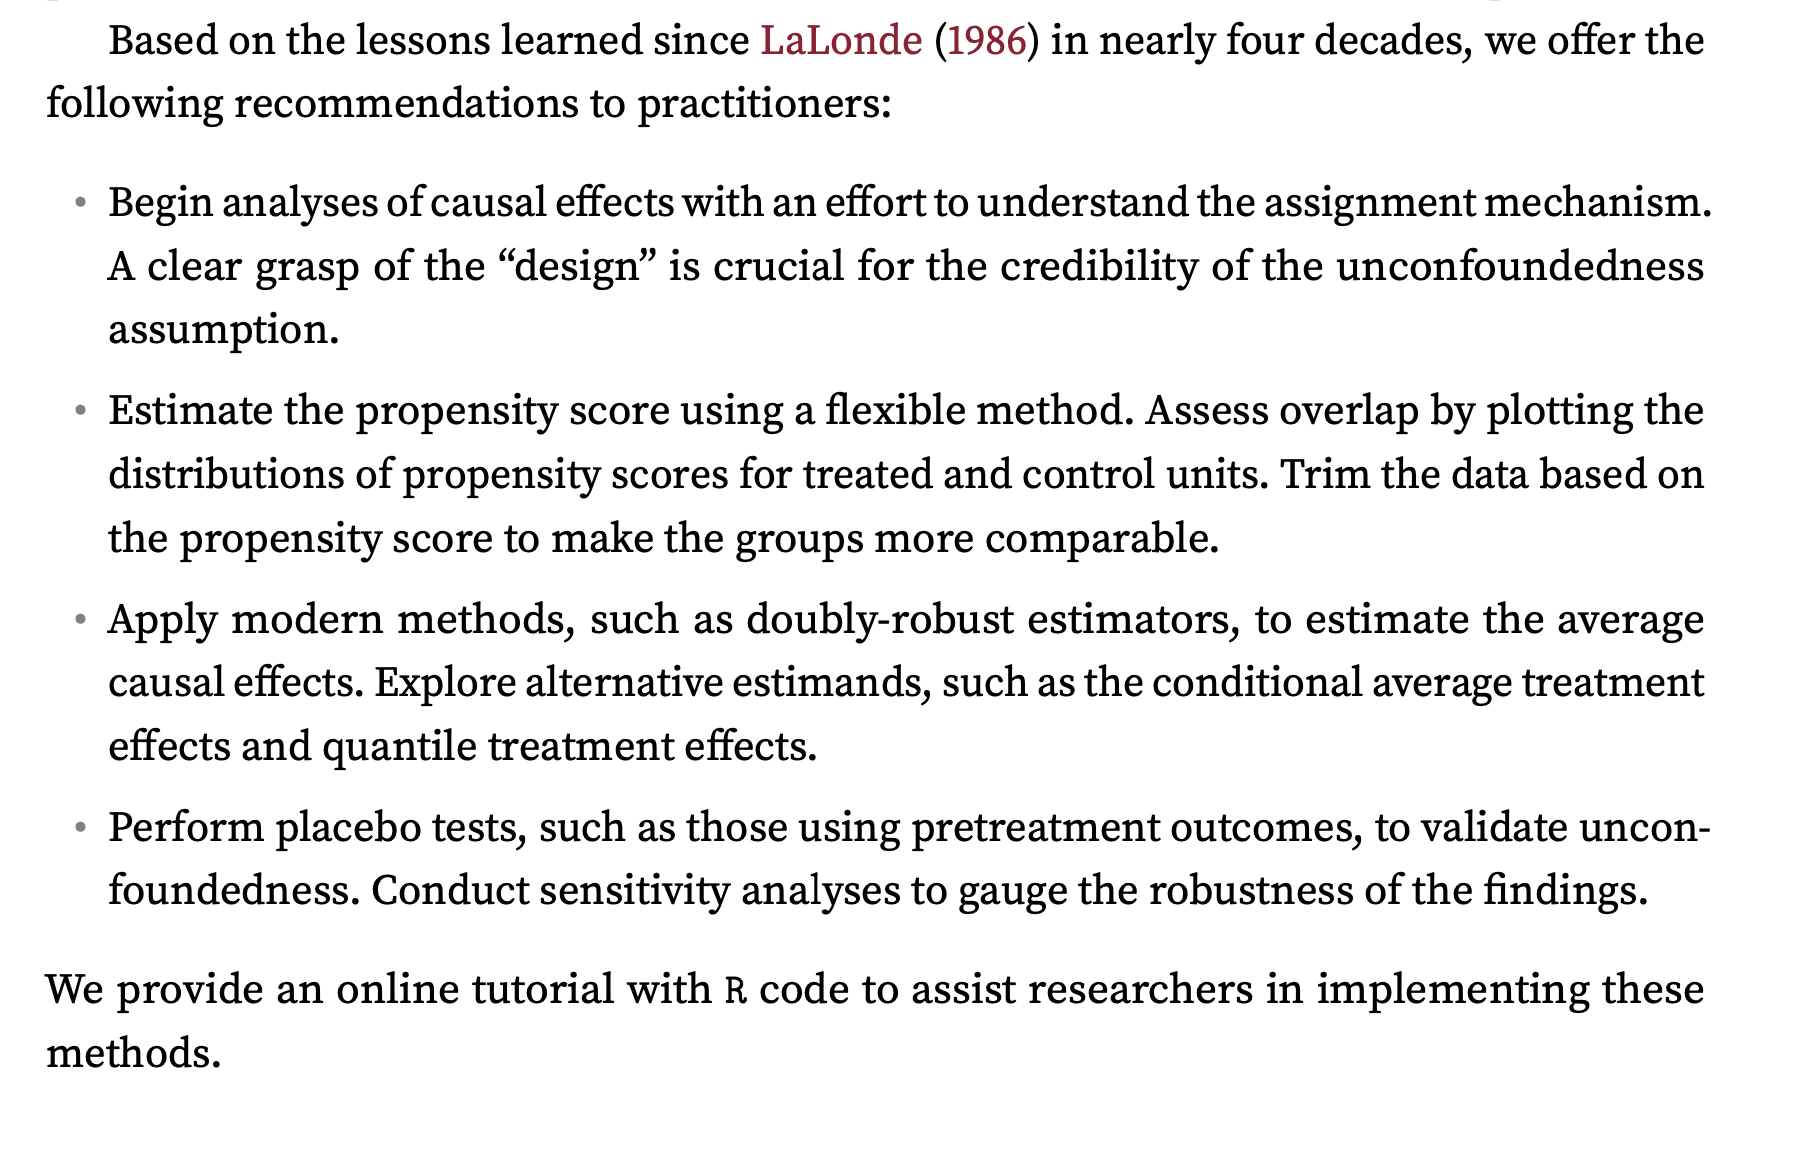
\includegraphics[scale=0.3]{./lecture_includes/imbens_xu_checklist}
  \end{figure}

\end{frame}


\begin{frame}{The curse of dimensionality bites before any estimator runs}

\begin{itemize}
\item It happens at the top layer --- in the raw cells of $X$, before you fit anything
\item Propensity scores \emph{summarize} the dimensions. They don't create matches
\item If there's no one-to-one match within $X$, a balancing method can mask that rather than fix it
\end{itemize}

\vspace{0.7em}

\begin{itemize}
\item When someone says they've handled it with a balancing weight, ask what the cells look like
\item \highlight{Always go look at the dimensions}
\end{itemize}

\end{frame}


\begin{frame}[plain]

\vspace{1.2em}
\begin{center}
{\Large Thank you}\\[0.6em]
\deemph{Northwestern, August 2026}
\end{center}

\vspace{1.4em}

\begin{itemize}
\item Slides, labs and data: \myurlshort{https://github.com/Mixtape-Sessions/Causal-Inference-1}{github.com/Mixtape-Sessions/Causal-Inference-1}
\item Imbens and Xu (2024) tutorial and code: \myurlshort{https://github.com/xuyiqing/lalonde}{github.com/xuyiqing/lalonde}
\end{itemize}

\vspace{0.8em}

\begin{center}
\deemph{scunning@gmail.com}
\end{center}

\end{frame}

\end{document}







